\documentclass[11pt]{report}
\usepackage{graphicx,multicol}
\usepackage[hidelinks]{hyperref}
\usepackage[Glenn]{fncychap}  % Custom chapter style
\usepackage[english]{babel}
\usepackage{fancyhdr}
\pagestyle{fancy}
\usepackage{colortbl}
%\usepackage[utf8]{inputenc}
\usepackage{amsmath}
\usepackage{geometry}
\usepackage{tikz}
\usepackage{setspace}
\usepackage{booktabs}
\usepackage{multicol}
\usepackage{float}
\usepackage{tocloft} 
\usepackage[backend=biber,style=apa]{biblatex}
\usepackage{booktabs} % For professional looking tables
\usepackage{tabularx} % For flexible column widths
\usepackage{geometry} % Adjust page margins if needed
\geometry{margin=1in}

\DeclareUnicodeCharacter{200B}{}



\usepackage[backend=biber,style=apa]{biblatex} % Utilisez le style APA ou un autre style selon les besoins
\addbibresource{references.bib} % Lien vers le fichier de bibliographie

%\lhead{\leftmark} % en-tête gauche-chapitre
\lhead{\rightmark} % en-tête gauche-section
\chead{} % en-tête centre
\rhead{\thepage} % en-tête droite-no de page
\lfoot{2024-2025} % pied gauche perso
\cfoot{3rd Year Meteorology} % pied centre perso
\rfoot{modeling project} % pied droit perso
\renewcommand{\headrulewidth}{2. pt}
\renewcommand{\footrulewidth}{2. pt}


\begin{document}



%\documentclass[12pt,a4paper]{report}
%\usepackage[Glenn]{fncychap}
%\usepackage[french]{babel}
%\usepackage{fancyhdr}
%\pagestyle{fancy}
%\usepackage{colortbl}
%\usepackage[utf8]{inputenc}
%\usepackage{graphicx}
%\usepackage{amsmath}
%\usepackage{hyperref}
%\usepackage{geometry}
%\usepackage{tikz}
%\usepackage{setspace}
%\usepackage{booktabs}
%\geometry{margin=1in}
%\usepackage{graphicx}
%\usepackage{booktabs}
%\usepackage{tabularx}
%\usepackage{amsmath}
%\usepackage{unicode-math}
%\usepackage{pifont}
%\usepackage{float}
%
%
%
%\usepackage[backend=biber,style=apa]{biblatex} % Utilisez le style APA ou un autre style selon les besoins
%\addbibresource{references.bib} % Lien vers le fichier de bibliographie
%
%%\lhead{\leftmark} % en-tête gauche-chapitre
%\lhead{\rightmark} % en-tête gauche-section
%\chead{} % en-tête centre
%\rhead{\thepage} % en-tête droite-no de page
%\lfoot{2024-2025} % pied gauche perso
%\cfoot{3rd Year Meteorology} % pied centre perso
%\rfoot{modeling project} % pied droit perso
%\renewcommand{\headrulewidth}{2. pt}
%\renewcommand{\footrulewidth}{2. pt}
%
%\begin{document}
\thispagestyle{empty} % Supprime les en-têtes et pieds de page pour cette page

\clearpage
\begin{titlepage}
  \begin{center}
    % Logos at the top
    
\includegraphics[width=0.15\textwidth]{DGM.jpg} \hfill
    
\includegraphics[width=0.25\textwidth]{ehtp.jpg} \\[2cm]

    
    % Colored lines above and below the main title
    \noindent\rule{\textwidth}{1mm}\\[0.5cm]
    {\LARGE \textbf{\textcolor{blue}{Evaluation of Climate Models For Seasonal Forecasting in the MENA Region\\ \vspace{0.1cm} 
   }}}
    \noindent\rule{\textwidth}{1mm}\\[3cm]
    \vfill
    % Author and supervisor
 \begin{center}
    \textbf{\large Prepared by:} \\[0.2cm]
    \textbf{Berrahmouch Nohayla and Mohamed El-Badri} \\[0.2cm]
    Hassania School of Public Works, Casablanca, Morocco \\[1.5cm]
    
    \textbf{\large Supervised by:}
\end{center}

\begin{tabbing}
    \hspace{6cm} \= \hspace{6cm} \= \kill 
    \textbf{Internal Supervisor:} \> \> \textbf{External Supervisors:} \\[0.5cm]
    \textbf{Mr. Driss Bari} \> \> \textbf{Mrs. Wafae Badi} \\[0.2cm]
    Hassania School of Public Works \\ 
    and Direction Générale de la Météorologie, Morocco \> \> DGM, Morocco \\[0.5cm]
    
    \> \> \textbf{Mr. Nicholas Savage} \\[0.2cm]
    \> \> Met Office, Exeter, UK \\
\end{tabbing}


    \vfill

    % Date
    {\large 2024 - 2025} \\[1cm]
  \end{center}
\end{titlepage}
\tableofcontents
\chapter*{Acknowledgments}
\addcontentsline{toc}{chapter}{Acknowledgments}
\vskip-3.3em  

We would like to express our deepest gratitude to \textbf{Mrs. Wafae Badi} for her unwavering support and invaluable guidance throughout this project. Her insightful counsel and constant encouragement enabled us to overcome various challenges and maintain our focus. Her dedication to fostering progress, coupled with her constructive feedback and open-minded approach, were instrumental in shaping the direction of this work. Her mentorship has truly been a cornerstone of our journey, and we are profoundly grateful for her invaluable contributions.  
\\

Special thanks go to \textbf{Mr. Nicholas Savage} and his exceptional team at the UK Met Office. Their generosity in sharing their expertise and resources provided us with unparalleled opportunities to broaden our understanding of climate modeling. The engaging discussions and valuable insights shared by Mr. Savage and his team not only enriched this project but also fueled our motivation to explore innovative avenues. Their commitment to advancing climate science inspired us to aim higher and achieve more.
\\

We are also immensely grateful to \textbf{Mr. Bari}, whose dedicated supervision, thoughtful suggestions, and constructive critiques significantly enhanced the quality of this work. His ability to balance critical feedback with motivating encouragement made a remarkable difference, guiding us through challenging moments and ensuring steady progress. 
\\

In addition, we would like to acknowledge the support received through the \textbf{WISER MENA project}. \textbf{Nicholas Savage’s time was funded via the WISER MENA project.} The Weather and Climate Information Services (WISER) Programme is funded with UK International Development from the UK government and led by the Met Office in the UK. This work has been partially supported by UK International Development from the UK government; however, the views expressed do not necessarily reflect the UK government’s official policies.  
\\

Lastly, we extend our heartfelt appreciation to all those who, directly or indirectly, contributed to this project. Your cooperation, guidance, and belief in our work have made this journey a fulfilling and enlightening experience. While this project is a testament to hard work and collaboration, it is also a reflection of the collective effort and support of everyone who believed in its success. To you, we owe our sincere thanks.

\chapter*{Preface}
\addcontentsline{toc}{chapter}{Preface}
\vskip-3.3em    
The MENA seasonal forecasting models have undergone both probabilistic and deterministic evaluations. This research study is regarded as the pioneering work and the first of its kind in this area which helps in situational context improvement in seasonal forecasting models. Given the alarming rate of increase in the impacts caused by extreme climatic events including severe droughts, and extreme heat and other climate sensitive issues in the MENA region, this work is a key contribution towards alleviating these issues=
\\

Due to climatic extremes in the MENA region, agriculture, human livelihood, and natural resources are heavily affected. Consequently, it has become almost necessary to have forecasts of seasons that are credible so as to characterize the impacts, or to enhance preparedness. Although seasonal forecasting models have been widely researched and practiced in many parts of the world, their use in MENA countries’ local level remains scarce. This gap is resolved in this study, providing new knowledge and tools for climate scientists working in the region.\\

In this work, we intend to broaden the knowledge fabric of climate change science by focusing on the climate change and variability vulnerability of the MENA region. The results obtained not only improve the comprehension of the dynamics of the local climate, but also lays a framework for specific approach to be employed for adaptation strategies.\\

We are immensely grateful to every individual or organization who has helped support this project and guided us through uncharted territory in the spectrum of MENA climate predictions.\\
\chapter{Overview and Rationale of the Study}
The last couple of decades have witnessed a surge in demand for seasonal climate forecasting. Global advancements in space science and technology have lead to the better anticipation of climate seasons up to a through range of 3-12 months. This is crucial for effective planning in major industries like agriculture or energy management, among others. These advancements breed an increased dependence on seasonal forecasting and in turn create a higher demand for accurate forecasting mechanisms. Therefore two central methodologies have witnessed prominence – deterministic and probabilistic methods. A hindsight understanding of these mechanisms is imperative, as they are useful for evaluating and understanding the shortcomings and effectiveness of different models employed in forecasting seasonal amps.\\

Probabilistic forecasts take one step forward, do not try to predict an ideal scenario and present different potential outcomes, each with a defined probability. Efforts, though different, instruct towards the same ends; meeting a specific operational/strategic need. Lorenz’s butterfly effect presents the case for one such endeavor- it shows how a non-linear system’s response can drastically alter depending on the initial conditions. Such chaos is especially present in weather and climate systems where even the slightest details can have large ramifications over longer periods.\\

In this context, the current study focuses on developing relationships that integrate conceptual advancements in seasonal forecasting efforts with practical and applicable methods. The geographical focus of this study is the **MENA region (Middle East and North Africa)**, a zone characterized by its diverse climatic conditions and critical socio-economic dependence on accurate seasonal forecasts. The MENA region is particularly vulnerable to climate variability due to its arid and semi-arid environments, limited water resources, and reliance on agriculture and energy. By analyzing seasonal forecasting within this region, the study seeks to address key challenges and contribute to sustainable climate-resilient solutions.\\




\chapter{Introduction}
\section{Context}
\subsection{Overview of Climate Modeling and Seasonal Forecasting}

Climate modeling is the process of using mathematical representations of the Earth’s atmosphere, oceans, land surface, and ice systems to simulate and predict climate dynamics. These models are based on fundamental physical principles, such as the conservation of mass, energy, and momentum, and are implemented through numerical methods that solve complex equations governing the interactions between these systems.\footnote{McGuffie, K. and Henderson-Sellers, A., 2014. A Climate Modelling Primer. \url{https://doi.org/10.1002/9781118687853}} Climate models range from global circulation models (GCMs), which simulate large-scale atmospheric and oceanic processes, to regional climate models (RCMs), which provide localized projections by incorporating finer-scale topographic and land-use details.\footnote{Flato et al., 2013. Evaluation of Climate Models. IPCC AR5 Chapter 9. \url{https://www.ipcc.ch/report/ar5/wg1/chapter-9-evaluation-of-climate-models/}} Seasonal forecasting, a subset of climate modeling, refers to the prediction of climate conditions, such as temperature and precipitation, over a period of one to six months. These forecasts rely on initial conditions (e.g., sea surface temperatures, soil moisture) and slowly varying components of the climate system, such as oceanic or atmospheric anomalies like the El Niño-Southern Oscillation (ENSO).\footnote{Doblas-Reyes, F. J., García-Serrano, J., Lienert, F., Biescas, A. P., \& Rodrigues, L. R., 2013. Seasonal climate predictability and forecasting: Status and prospects. \url{https://doi.org/10.1038/ngeo1714}} The basic principle behind seasonal forecasting is to leverage these slowly varying components, which have a predictable influence on regional weather patterns, using ensemble simulations to quantify uncertainties and provide probabilistic predictions.\footnote{Palmer, T. N., \& Anderson, D. L., 1994. The prospects for seasonal forecasting—a review paper. \url{https://doi.org/10.1256/smsqj.50402}}  

Seasonal forecasts play a crucial role in decision-making and planning across various sectors, including agriculture, water management, and climate risk mitigation. These forecasts provide early warnings of high-impact climate scenarios, enabling proactive decisions that result in financial savings, risk reduction, and optimized resource use. For instance, in agriculture, they assist farmers in selecting appropriate crops and determining optimal planting times based on anticipated water availability, thereby mitigating risks associated with droughts or excessive rainfall.\footnote{Werner, M. and Linés, C., 2024. Seasonal forecasts to support cropping decisions. \url{https://doi.org/10.5194/egusphere-egu24-13436}} Seasonal forecasts also support pre-harvest strategies, such as hedging decisions, which help shield farmers from price volatility, although their adoption is often hindered by perceptions of inaccuracy and complexity.\footnote{Hunt et al., 2020. Seasonal Forecast Based Preharvest Hedging. \url{https://doi.org/10.22004/AG.ECON.309761}} In water management, seasonal forecasts are vital for mitigating drought impacts, particularly in semi-arid regions, by enabling improved reservoir operations and efficient water allocation to reduce losses.\footnote{Portele et al., 2021. Seasonal forecasts offer economic benefits for hydrological decision-making. \url{https://doi.org/10.1038/s41598-021-89564-y}} Additionally, these forecasts, when linked to hydrological models, improve predictions of water balance and inform critical decisions regarding water storage and distribution, despite occasional discrepancies between predicted and desired variables.\footnote{MacLeod et al., 2023. Translating seasonal climate forecasts into water balance forecasts. \url{https://doi.org/10.1371/journal.pclm.0000138}} Seasonal forecasts are increasingly applied in climate risk management, where they help predict extreme weather events, providing decision-makers with tools to minimize societal and economic damages.\footnote{Castino et al., 2023. Towards seasonal prediction of extreme temperature indices. \url{https://doi.org/10.5194/ems2023-590}} For example, accurate predictions of heatwaves or floods allow authorities to implement adaptive measures, reducing infrastructure damage and safeguarding public health. In economic sectors such as energy and water management, tailored seasonal forecasts enhance decision-making efficiency by aligning forecasts with user needs, thereby optimizing outcomes.\footnote{Goodess et al., 2022. The Value-Add of Tailored Seasonal Forecast Information. \url{https://doi.org/10.3390/cli10100152}} Despite their significant potential, the effectiveness of seasonal forecasts depends on their accuracy, relevance to user needs, and ease of use. Improved communication, stakeholder training, and efforts to bridge the gap between forecast complexity and user understanding are essential to maximize their utility.



\subsection{Importance of Seasonal Climate Forecasts in MENA}
Seasonal climate forecasts are critically important across the MENA region, where high temperatures, low water availability, and vulnerability to climate variability create substantial challenges for sustainable development. Forecasts provide early warnings of droughts, heatwaves, and other extreme weather events, enabling decision-makers to implement proactive measures to mitigate impacts on water resources, agriculture, and infrastructure.\footnote{Dunn et al., 2020. The changing climate of MENA. \url{https://pubs.giss.nasa.gov/abs/gu00200u.html}} In agriculture, these forecasts help farmers optimize crop selection and planting schedules, reducing the risks of crop failure in this water-scarce region.\footnote{Werner, M., and Linés, C., 2024. Seasonal forecasts to support cropping decisions. \url{https://doi.org/10.5194/egusphere-egu24-13436}} In the water sector, seasonal forecasts guide reservoir management by predicting rainfall variability, improving water storage strategies, and ensuring more equitable water distribution.\footnote{Portele et al., 2021. Seasonal forecasts for hydrological decision-making. \url{https://doi.org/10.1038/s41598-021-89564-y}} With increasing climate risks, these forecasts also support disaster risk management by allowing governments to prepare for extreme events, such as heatwaves and floods, which are becoming more frequent in the region due to climate change.\footnote{Castino et al., 2023. Towards seasonal prediction of extreme temperature indices. \url{https://doi.org/10.5194/ems2023-590}} Moreover, the economic benefits of using seasonal forecasts are significant. By enabling energy companies to anticipate peak demand periods driven by heatwaves, and by helping municipalities optimize water usage during droughts, these forecasts provide cost savings and efficiency gains.\footnote{Goodess et al., 2022. Value-Add of tailored seasonal forecast information. \url{https://doi.org/10.3390/cli10100152}} However, challenges persist in ensuring the accuracy and usability of these forecasts. The arid and semi-arid nature of much of the MENA region, coupled with complex interactions between regional climate drivers, makes it difficult to provide highly localized forecasts.\footnote{Latif et al., 2011. ENSO predictability and regional climate impacts. \url{https://doi.org/10.1175/2010JCLI3405.1}} Addressing these challenges through improved modeling techniques and stakeholder engagement will be critical to maximizing the value of seasonal forecasts in the MENA region, ensuring better preparedness and resilience against a changing climate.


\section{Objectives of the Work and Description of Report Content}
The primary objective of this work is to evaluate the effectiveness of climate models, focusing specifically on their performance in predicting key climate variables such as temperature, precipitation. This evaluation incorporates both deterministic and probabilistic approaches to identify the most skillful models and their suitability for practical applications.

\subsection{Specific aims  of evaluating deterministic and probabilistic models.
}
The evaluation of deterministic and probabilistic models is essential for understanding their unique strengths, limitations, and potential applications in diverse fields. Deterministic models, which generate a single, precise outcome based on initial conditions, are widely used when exactness and reproducibility are critical, such as in engineering and physical simulations.\footnote{McGuffie, K., and Henderson-Sellers, A., 2014. *A Climate Modelling Primer*. Wiley. \url{https://doi.org/10.1002/9781118687870}} Their evaluation focuses on assessing accuracy and reliability under specific conditions, providing clarity in cause-and-effect relationships. In contrast, probabilistic models incorporate uncertainty by assigning probabilities to various potential outcomes, enabling the representation of real-world complexities and variability.\footnote{Palmer, T., and Hagedorn, R., 2006. *Predictability of Weather and Climate*. Cambridge University Press. \url{https://doi.org/10.1017/CBO9780511617652}} These models are particularly beneficial for strategic planning and risk management, where understanding a range of possible scenarios is crucial. The evaluation of both types of models includes conducting sensitivity analyses to determine how changes in input variables affect outcomes, which helps in identifying key drivers of uncertainty and improving model performance.\footnote{Seneviratne, S.I., et al., 2021. *Metrics for climate model evaluation: A review*. Nature Communications. \url{https://doi.org/10.1038/s43247-021-00094-x}} Additionally, risk assessment is a vital component, with deterministic approaches offering straightforward estimations for defined scenarios, while probabilistic approaches address uncertainties by simulating a spectrum of possible outcomes.\footnote{PreventionWeb, 2021. *Deterministic and Probabilistic Risk*. \url{https://www.preventionweb.net/understanding-disaster-risk/key-concepts/deterministic-probabilistic-risk}} These evaluations also aim to support decision-making processes by identifying which type of model is more appropriate for specific contexts—deterministic models for precise predictions and probabilistic models for flexible planning under uncertainty.\footnote{Goodess, C.M., et al., 2022. *The Value-Add of Tailored Seasonal Forecast Information for Industry Decision Making*. Climate. \url{https://doi.org/10.3390/cli10100152}} Finally, probabilistic models are often recognized for their adaptability in dynamic environments, as they can incorporate new data and adjust probability distributions to reflect evolving conditions, making them indispensable for complex systems where deterministic models may fall short.\footnote{Latif, M., and Keenlyside, N., 2011. *El Niño/Southern Oscillation Predictability*. Journal of Climate. \url{https://doi.org/10.1175/2010JCLI3405.1}} Together, the evaluation of deterministic and probabilistic models provides invaluable insights into their suitability for addressing specific challenges, supporting informed decision-making, and advancing model development.

\subsection{Description of Content}

This report is designed to provide a comprehensive analysis of climate model evaluation, focusing on both deterministic and probabilistic approaches. The structure of the report follows a logical progression, starting with an introduction to the fundamental concepts behind climate models. The first section lays the groundwork for understanding the key differences between deterministic and probabilistic models, describing how each approach is used to simulate climate systems and predict future outcomes. The methodology chapter follows, detailing the specific techniques employed to assess the models. This includes the use of both deterministic and probabilistic metrics such as Root Mean Square Error (RMSE), Anomaly Correlation Coefficient (ACC), and Brier Score, which are critical for evaluating the models' accuracy and performance in predicting climate variables like temperature and precipitation.

Next, the report moves on to the results and analysis, where the performance of the selected models is presented and compared. This section highlights the models' strengths and weaknesses, providing insight into how well they predict climate patterns across various geographical regions and time periods. Special attention is given to the models' skill in forecasting extreme weather events, which are particularly relevant to sectors like agriculture, water resource management, and disaster risk reduction.

The final section of the report provides conclusions and recommendations based on the analysis. This chapter synthesizes the findings, offering practical suggestions for improving the accuracy, usability, and application of climate forecasts. Recommendations also address how future developments in climate modeling can better meet the needs of decision-makers and stakeholders. The report as a whole seeks to contribute valuable insights into the ongoing development of climate prediction systems, aiming to enhance their effectiveness in real-world applications.


\chapter{Literature Review}
\section{Overview of Climate Models}
\subsection{Deterministic Models}
Deterministic models rely on mathematical equations that describe the physical processes of the atmosphere. These models use fixed initial conditions to provide precise predictions, making them suitable for short-term forecasting. However, due to the chaotic nature of atmospheric systems, as demonstrated by Lorenz's theorem, deterministic models are limited in their ability to predict long-term outcomes. Small errors in initial conditions can lead to significant differences in results, reducing their reliability for seasonal or long-term forecasting.\footnote{Lorenz, E. N. (1963). Deterministic Nonperiodic 
Flow. \textit{Journal of the Atmospheric Sciences, 20}(2), 130–141.}

Deterministic climate models operate based on fixed initial conditions and mathematical equations that simulate physical processes in the atmosphere. These models are particularly useful for short-term predictions as they provide precise and singular forecasts. However, deterministic models are significantly limited when forecasting over extended periods. This limitation arises due to the inherent sensitivity of atmospheric systems to initial conditions—a concept known as the \textit{butterfly effect}, introduced by Edward Lorenz in 1963. His research demonstrated that even minute changes in the initial conditions of a system could lead to vastly different outcomes over time, emphasizing the chaotic nature of weather systems.

For seasonal forecasting, deterministic models often fail because minor errors in the initial conditions can amplify, resulting in inaccurate predictions for longer timescales. Despite these challenges, deterministic models are vital for understanding specific phenomena over shorter durations with high spatial and temporal resolution.




\subsection{Probabilistic Models}
Probabilistic models address the limitations of deterministic approaches by incorporating uncertainty into forecasts. Instead of producing a single outcome, these models generate a range of possible scenarios, each with an associated probability, using ensemble simulations or statistical techniques. This makes probabilistic models particularly useful for medium- to long-term forecasts and risk assessment in climate-sensitive sectors such as agriculture, water management, and disaster mitigation.\footnote{World Meteorological Organization (2024). \textit{Guidance on Verification of Operational Seasonal Climate Forecasts}. \url{https://library.wmo.int/records/item/56227-guidance-on-verification-of-operational-seasonal-climate-forecasts}}

The evaluation of probabilistic models relies on metrics that assess their ability to represent uncertainty and provide actionable insights:
\begin{itemize}
    \item \textbf{Reliability:} Measures how well predicted probabilities align with observed frequencies.
    \item \textbf{Resolution:} Assesses the model’s ability to distinguish between different outcomes.
    \item \textbf{Discrimination:} Evaluates the model’s ability to separate events from non-events.\footnote{Rapport de projet 2024–2025, \textit{3rd Year Meteorology Modeling Project}.}
\end{itemize}

Probabilistic models are especially valuable for decision-making under uncertainty, as they provide stakeholders with a clearer understanding of risks and potential scenarios, enabling proactive measures to mitigate impacts.

\subsubsection{Comparison of Deterministic and Probabilistic Models}
Deterministic and probabilistic models serve complementary roles in climate modeling and forecasting. Their distinct features and applications are summarized in Table~\ref{tab:comparison_models}.

\begin{table}[h!]
    \centering
    \caption{Comparison of Deterministic and Probabilistic Models}
    \begin{tabular}{@{}p{5cm}p{5cm}p{5cm}@{}}
    \toprule
    \textbf{Feature} \& \textbf{Deterministic Models} \& \textbf{Probabilistic Models} \\
    \midrule
    Predictability \& Produces a single fixed outcome based on initial conditions \& Generates a range of outcomes with associated probabilities \\
    \addlinespace
    Sensitivity to Initial Conditions \& Highly sensitive, leading to reduced accuracy over long timeframes \& Less sensitive due to ensemble techniques reducing error amplification \\
    \addlinespace
    Application Domain \& Suitable for short-term, high-resolution tasks, e.g., extreme event analysis \& Ideal for medium- and long-term decision-making under uncertainty \\
    \addlinespace
    Use of Historical Data \& Limited emphasis on historical variability \& Extensively relies on historical data for statistical projections \\
    \addlinespace
    Examples \& Global Circulation Models (GCMs), Regional Climate Models (RCMs) \& Ensemble forecasting, statistical downscaling \\
    \bottomrule
    \end{tabular}
\end{table}

\noindent While deterministic models are preferred for precise and short-term predictions, probabilistic models provide critical insights into the likelihood of various scenarios, making them indispensable for managing climate-related risks.
\subsection{ STUDIES IN "MENA" REGION }
\subsubsection{The current and changing climate in MENA}
Much \footnote{\href{https://www.metoffice.gov.uk/binaries/content/assets/metofficegovuk/pdf/business/international/wiser/wiser-mena-scoping-study-external-v2.pdf}{Met Office WISER Report}} of the MENA region is characterised by high temperature and low water availability, a
combination of variables that have the potential to lead towards the environmental
limits/threshold for safe human habitation. This makes the region
particularly vulnerable to climate change and climate variability, as small variations in climate
can easily produce high temperatures or extensive droughts that are harmful to human lives
and livelihoods.\\

Changes in temperature and rainfall patterns have already been observed in the region and
are expected to change further in the near future, especially if global warming exceeds 1.5 to
2 °C above the pre-industrial level. Annual mean temperatures across the MENA region
have increased between 0.3–0.5°C per decade1 over the period 1980–2015 \footnote{\href{https://pubs.giss.nasa.gov/abs/gu00200u.html}{(Gutiérrez et al.,
2021)}}. Since the 1950s, hot and cold extremes have become warmer, the number of cold
days has decreased, and the number of warm days has increased (Dunn et al., 2020). There
has been an increase in heat waves intensity, frequency and duration    \footnote{\href{https://www.nature.com/articles/s41467-020-16970-7}{(Perkins-Kirkpatrick
and Lewis, 2020)}}. Annual mean precipitation shows a high level of spatial variability over the
MENA region. During the period 1980–2015 there have been downward trends in mean
annual precipitation \footnote{\href{https://pubs.giss.nasa.gov/abs/gu00200u.html}{(Gutiérrez et al., 2021)}} . Dry conditions, drought intensity and frequency
has increased in the past over the region \footnote{\href{https://www.nature.com/articles/s43247-021-00094-x}{(Seneviratne et al., 2021).}} 



\subsubsection{Impact-Based Evaluation}
Impact-based forecasting refers to a type of weather or climate forecasting that goes beyond predicting the meteorological parameters (e.g., temperature, rainfall, wind speed) and instead focuses on predicting the potential impacts of those conditions on society, infrastructure, and ecosystems. The goal is to provide actionable insights that help communities and decision-makers prepare for and mitigate the effects of extreme weather and climate events.

\textbf{Evaluation of Seasonal Forecast Models}\\
An impact-based evaluation\footnote{\url{https://agupubs.onlinelibrary.wiley.com/doi/full/10.1029/2024EF004936 }} \footnote{Zahir Nikraftar, Rendani Mbuvha, Mojtaba Sadegh, Willem A. Landman} was conducted as global study on five seasonal forecast models to identify the most effective for extreme precipitation forecasting (focuses on regions which were vulnerable to wildfire and flooding). The models assessed included:
\begin{itemize}
    \item Centro Euro‐Mediterraneo sui Cambiamenti Climatici (CMCC: version 35),
    \item Deutscher Wetterdienst (DWD: version 21),
    \item Environment and Climate Change Canada (ECCC: version 3),
    \item Météo‐France (version 8),
    \item UK Met Office (UK‐Met: version 601).
\end{itemize}

The findings highlighted the \textbf{\textit{UK‐Met} }  and \textbf{\textit{Météo‐France} } models as consistently superior across all four seasons. Meanwhile, the ECCC and CMCC models exhibited strong performance on specific indices and in particular regions, ranking just below the top two models.

\textbf{ROC Scores and Regional Performance}\\
The ROC scores indicate that forecast models perform exceptionally well in tropical and subtropical regions. This result is consistent with our study and can be attributed to the general predictability of oceanic conditions and the influence of climate drivers such as the El Niño-Southern Oscillation (ENSO). The Météo‐France and UK‐Met models exhibited superior performance during the SON and MAM seasons.

However, the prevalence of grids with no discrimination ROC categories is more common in extratropical regions. This can be attributed to:
\begin{itemize}
    \item Lower predictability of extratropical variations,
    \item Model limitations in capturing interactions between tropical and extratropical regions,
    \item Challenges in representing land surface processes (De Andrade et al., 2019).
\end{itemize}
The CMCC, DWD, and ECCC models often fail to detect extreme events in many extratropical areas, underscoring the stronger performance of the UK‐Met and Météo‐France models in these scenarios.

\textbf{Percent Bias Analysis}\\
The analysis of Percent Bias across four seasons demonstrates a consistent underestimation by forecast models for most extreme wet precipitation indices. Key observations include:
\begin{itemize}
    \item Forecast models underestimate extreme wet precipitation indices while overestimating light precipitation.
    \item Models perform better in capturing the intensity and magnitude of extreme events (e.g., highest daily and multi-day rainfall) compared to the frequency of wet or dry days.
\end{itemize}

In tropical and subtropical regions, models like \textbf{\textit{UK‐Met}}  and \textbf{\textit{Météo‐France} } exhibit strong performance due to their ability to capture large-scale climate patterns. In contrast, extratropical regions show higher biases, reflecting challenges in modeling complex interactions and seasonal variations.

\textbf{Global Model Comparison}\\
The \textbf{\textit{UK‐Met}} model consistently demonstrates lower biases and stronger performance globally compared to the \textbf{\textit{Météo‐France} }  model, highlighting its effectiveness in representing climate patterns. However, all models show limitations in accurately modeling persistent extreme wet and dry periods, particularly in extratropical areas.


\subsubsection{SYSTEM 7 FRANCE}

seasonal forecasting evaluation has been the subject of numerous studies, with a focus on improving the accuracy and reliability of predictions related to precipitation and other weather parameters. One such study\footnote{https://www.mdpi.com/2674-0494/1/3/16} conducted a probabilistic evaluation of seasonal precipitation re-forecasting from May to November over a period of 23 years (1993–2015). The study utilized the Brier Score (BS) and its decomposition to assess forecast performance, with the aim of providing more reliable and actionable predictions for extreme weather events.

The evaluation was conducted on the operational seasonal forecasting system of Meteo-France, which used 25 ensemble members, perturbed model dynamics, and initial conditions. The system aimed to provide a more detailed probabilistic forecast, in addition to existing deterministic metrics, for both seasonal and intra-seasonal forecasts. The BS was estimated using tercile probabilities and a non-parametric counting estimator, with the GPCP\footnote{Global Precipitation Climatology Project (GPCP)} observation data serving as the reference.

Multiple analyses were performed to evaluate the robustness of the BS score, revealing that spatial distributions of the BS can vary significantly based on the sampling methods, reference data, and ensemble types used. The analysis showed that large errors, especially in the tropical ocean, could be reduced by using hindcast ensemble climatological samples. In particular, errors over the Nino region in the Pacific Ocean could be mitigated using these methods. This highlights the importance of employing various ensemble data sources and reference climatology to enhance the reliability of seasonal forecasts.

A notable finding was the reduction in BS when using ensemble observations, especially in the tropical ocean, suggesting that increasing ensemble size can improve forecast accuracy up to a point. However, this was not the case in all regions, as some areas, such as the tropical Indian Ocean, exhibited high BS even with different analysis methods. The study also found that intra-seasonal analyses showed similar patterns to seasonal hindcasts, but with higher BS due to reduced sample sizes, highlighting the need for higher-resolution models and improved initial conditions.

The study concluded that, despite improvements, probabilistic forecasting still faces challenges, particularly in the tropical regions, where errors fluctuate with lead time. The study emphasized the need for continued development of forecasting methods, particularly in reducing uncertainties in evaluation scores. Future evaluations should expand beyond the BS to include other metrics, such as the forecast skill score and the relative operating characteristic (ROC), to better assess forecast performance and identify system deficiencies.

This study's findings underline the importance of ensemble forecasting and the use of diverse data sources to improve the accuracy of seasonal precipitation forecasts, particularly in tropical regions where predictability remains challenging.


\subsection{Evaluation Approaches}


In the WMO\footnotemark{} \footnotetext{https://library.wmo.int/records/item/56227-guidance-on-verification-of-operational-seasonal-climate-forecasts}. Guide, several criteria are provided for evaluating a good forecast. Each criterion offers insight into specific aspects of the model but cannot, on its own, fully determine the forecast's quality. By combining all the criteria, we can comprehensively assess the performance of the model.	 
		\subsubsection{Resolution}
	Resolution measures whether the outcome differs given different forecasts, while discrimination measures whether the forecasts differ given different outcomes.

Discrimination looks at how well your forecast separates cases when the event (outcome) happens (pass) from when it doesn’t happen (fail). It’s about telling apart the events.
Resolution looks at how well your forecast adapts to different situations, giving distinct probabilities for different cases. It’s about adjusting to the situation.

Resolution measures how well a forecast distinguishes between different outcomes. A forecast has high resolution if the predicted probabilities vary significantly depending on the actual outcome. In other words, resolution tells us whether the forecast changes (e.g., gives different probabilities) when the actual outcome changes.
High resolution: The forecast gives distinct and varying probabilities when different events (outcomes) occur. For example, if in one case the forecast predicts a high probability of rain and it rains, and in another case predicts a low probability and it doesn’t rain, the forecast shows good resolution.
Low resolution: If the forecast probabilities don’t change much regardless of whether it rains or not (e.g., always predicting a 50\% chance of rain), the forecast has poor resolution because it fails to capture the differences in actual outcomes.
Resolution can be determined by measuring how strongly the outcome is conditioned upon the forecast.
If the outcome is independent of the forecast, the forecast has no resolution and is useless
Forecasts with no resolution are neither “good” nor “bad”, but are useless. 
Metrics of resolution distinguish between potentially useful and useless forecasts, but not all these metrics distinguish between “good” and “bad” forecasts.

The following equation represents the "resolution" component of the Brier Score (BS) decomposition, which quantifies how well a set of probability forecasts differentiates between events and non-events:

\begin{equation}
\textbf {Resolution} = \frac{1}{n} \sum_{k=1}^{d} n_k \left( \bar{y}_k - \bar{y} \right)^2
\end{equation}

where:

\begin{equation}
\bar{y}_k = \frac{1}{n_k} \sum_{i=1}^{n_k} y_{k,i}
\end{equation}

\begin{itemize}
    \item $n$ is the total number of forecasts,
    \item $d$ is the number of discrete probability bins,
    \item $n_k$ is the number of forecasts in the $k$-th bin,
    \item $\bar{y}_k$ is the observed relative frequency for the $k$-th probability bin,
    \item $\bar{y}$ is the overall observed relative frequency.
\end{itemize}

The term $\left( \bar{y}_k - \bar{y} \right)^2$ captures the variance between individual forecast categories and the overall event frequency. Higher resolution indicates that forecasts better differentiate between events and non-events.\\
so the resolution tells us how the model change with different situations.\\
the scores used to evaluate resolution are Brier Score and Reliability.



		\subsubsection{Discrimination}

Discrimination measures how well the forecast separates cases where the event occurs from cases where it does not. In other words, it examines whether the forecast probabilities differ for events that happen versus those that don't.
High discrimination: A forecast has high discrimination if, for example, when rain occurs, the forecast consistently predicts a high probability of rain, and when rain doesn’t occur, it predicts a low probability. It means the forecast is good at distinguishing between rain and no-rain days.
Low discrimination: If the forecast provides similar probabilities regardless of whether it rains or not (e.g., predicting a 60\% chance of rain every day), it has poor discrimination because it doesn’t effectively differentiate between days with and without rain. The score used to evaluate descrimination is ROC\footnote{Relative operating characteristics}.
		\subsubsection{Reliability}

A forecast is reliable if the predicted probabilities match the actual frequencies. For instance:
If you forecast a 40\% probability for below-normal rainfall, below-normal rainfall should occur in 40\% of the cases where you make that prediction.
Similarly, if you forecast a 25\% chance of above-normal rainfall, above-normal rainfall should happen 25\% of the time when you give that probability.
If this relationship holds consistently over many forecasts, the forecasts are well-calibrated (or reliable).
A Reliable but Uninformative Forecast
A forecast that always gives the climatological probability (e.g., always predicting a 33\% chance for each category: below, normal, above normal) would be reliable because the climatological average matches the observed frequencies. However, this forecast wouldn’t provide any information about changing conditions from case to case—it doesn’t adapt to the current situation, making it uninformative.

\begin{equation}
\textbf{Reliability} = \frac{1}{n} \sum_{k=1}^{d} n_k \left( \bar{p}_k - \bar{y}_k \right)^2
\end{equation}


\begin{itemize}
    \item $n$ is the total number of forecasts,
    \item $d$ is the number of discrete probability bins,
    \item $n_k$ is the number of forecasts in the $k$-th bin,
    \item $\bar{y}_k$ is the observed relative frequency for the $k$-th probability bin,
    \item $\bar{p}_k$ is relative frequency for the $k$-th probability.
\end{itemize}


		\subsubsection{Sharpness}
Sharp forecasts provide a strong signal about the expected outcome. For example, a sharp forecast might assign a 70\% chance to a certain outcome, like above-normal rainfall. This high probability communicates more confidence in that specific outcome.
On the other hand, when the forecast probabilities are close to the climatological values (like assigning a 40\% chance to above-normal, 35\% to normal, and 25\% to below-normal), the forecast is not very sharp, meaning the forecaster isn't very confident in predicting any one outcome.
The climatological probabilities are reliable, but aren’t sharp.
\section{Methodology}

\subsection{DATA}

The hindcast data used in this study was obtained using the OSOP package\footnote{https://github.com/OSFTools/osop/tree/main/scripts}, a tool developed by the UK Met Office to facilitate the retrieval of climate and meteorological data. The dataset comprises monthly mean seasonal forecasts for temperature over the MENA (Middle East and North Africa) region.


The hindcast data spans the common period 1993–2016 and was downloaded from the Copernicus Climate Change Service (C3S) platform. 


The data was retrieved for the following configurations:
\begin{itemize}
	\item Variable: 2-meter air temperature (t2m).
	\item Forecast Range: Lead times of interest (1–3 months), it includes DJF\footnote{December,January,February}, JJA\footnote{June,July,August}, MAM\footnote{March,April,May}, SON\footnote{September,October,November}
	\item Geographical Area: MENA region.
	\item Temporal Coverage: 1993–2016
	\item the used centers are $UKMO,ECMWF,ECCC_2,ECCC_3,CMCC,Meteo-France_8,DWD$
\end{itemize}


In addition to the hindcast data, this study utilized ERA5 reanalysis data, a state-of-the-art atmospheric reanalysis product produced by the European Centre for Medium-Range Weather Forecasts (ECMWF). 

    

\subsection{Deterministic Evaluation Metrics}
To evaluate the performance of seasonal climate prediction models, a range of deterministic measures is employed. These metrics offer valuable insights into the accuracy and reliability of forecasts by assessing the alignment between predicted and observed values. In this section, we present the main deterministic measures, which will also be applied in our study.
\subsubsection{Deterministic Measures}

Deterministic measures are statistical metrics used to assess the accuracy and reliability of climate forecasting models. These measures quantify the degree of correspondence between the predicted (Hindcast) and observed (Observation) values. Below, we present some widely used deterministic measures.

\subsubsection{Spearman Rank Correlation}

Spearman's correlation is a non-parametric measure of rank correlation, assessing the statistical dependence between the rankings of two variables. It evaluates how well the relationship between two variables can be described using a monotonic function, irrespective of whether it is linear or not. 

\[
r_s = \frac{\text{cov}(R[H], R[O])}{\sigma_{R[H]} \cdot \sigma_{R[O]}}
\]

where:  
\begin{itemize}
    \item \( r_s \): Spearman rank correlation.  
    \item \( H \): The Hindcast.  
    \item \( O \): The Observation.  
    \item \( R[x] \): The rank of the variable \( x \).  
    \item \( \sigma_x \): Standard deviation of the variable \( x \).  
\end{itemize}


Spearman correlation is particularly useful as it focuses on the rankings rather than the actual values, making it effective for evaluating monotonic relationships in seasonal forecasting models. Its interpretation provides valuable insights into the nature and strength of the relationship between hindcasts and observations:  

\begin{itemize}
    \item A positive Spearman correlation (\( r_s > 0 \)) indicates that the ranks of the hindcast and observation move in the same direction, showing a consistent relationship.  
    \item A negative Spearman correlation (\( r_s < 0 \)) suggests that as the rank of one variable increases, the rank of the other decreases, indicating an inverse relationship.  
    \item A Spearman correlation close to 0 (\( r_s \approx 0 \)) implies little to no monotonic relationship between the hindcast and observation.  
    \item A Spearman correlation close to +1 or -1 (\( r_s \approx \pm1 \)) demonstrates a strong monotonic relationship, regardless of whether it is linear or not.  
\end{itemize}
\subsubsection{Root Mean Square Error (RMSE)}

The RMSE measures the average magnitude of error between the hindcast and observed values. It is a robust metric to assess the overall predictive accuracy of a model. 

\[
RMSE = \sqrt{\frac{1}{n} \sum_{i=1}^{n}(H_i - O_i)^2}
\]

where:  
\begin{itemize}
    \item \( H \): The Hindcast.  
    \item \( O \): The Observation.  
    \item \( i \): The valid time (index of the data point).  
\end{itemize}


The interpretation of RMSE provides insights into the model's accuracy:  
\begin{itemize}
    \item A lower RMSE indicates higher accuracy, meaning the hindcast values are closer to the observed values.  
    \item A higher RMSE suggests larger discrepancies between predictions and observations, indicating lower model accuracy.  
    \item RMSE is useful for comparing the performance of different models or forecasting methods.  
\end{itemize}


\subsubsection{Coefficient of Determination (\( R^2 \))}
The coefficient of determination, \( R^2 \), evaluates the goodness of fit of a model. It measures the proportion of variance in the observed data that is explained by the model's predictions. An \( R^2 \) value closer to 1 indicates better predictive performance, while values near 0 suggest a weak relationship. 

\[
R^2 = 1 - \frac{\sum_{i=1}^n (O_i - H_i)^2}{\sum_{i=1}^n (O_i - \bar{O})^2}
\]

where:  
\begin{itemize}
    \item \( R^2 \): Coefficient of determination.  
    \item \( H_i \): Predicted value (Hindcast).  
    \item \( O_i \): Observed value (Observation).  
    \item \( \bar{O} \): Mean of the observed values.  
    \item \( \sum_{i=1}^n (O_i - H_i)^2 \): Residual sum of squares (unexplained variance).  
    \item \( \sum_{i=1}^n (O_i - \bar{O})^2 \): Total sum of squares (total variance).  
\end{itemize}

The interpretation of \( R^2 \) provides insights into the model's performance:  
\begin{itemize}
    \item A higher \( R^2 \) (closer to 1) indicates that a large proportion of the variance in the observations is explained by the model, signifying better predictive accuracy.  
    \item A lower \( R^2 \) (closer to 0) suggests that the model fails to explain much of the variance, indicating poor model performance.  
    \item \( R^2 \) is a useful metric for comparing different models and understanding how well each model captures the variability in the observed data.  
\end{itemize}

\subsubsection{Anomaly Correlation Coefficient (ACC)}

The Anomaly Correlation Coefficient (ACC) evaluates the skill of seasonal forecasts by comparing anomalies (deviations from climatology) between hindcasts and observations. It considers both the direction and magnitude of the anomalies, making it a robust metric for assessing forecast accuracy in climate studies.

\[
ACC = \frac{\sum_{i=1}^{n} (H_i - \bar{H})(O_i - \bar{O})}{\sqrt{\sum_{i=1}^{n} (H_i - \bar{H})^2 \cdot \sum_{i=1}^{n} (O_i - \bar{O})^2}}
\]

where:  
\begin{itemize}
    \item \( ACC \): Anomaly Correlation Coefficient.  
    \item \( H_i \): Forecast anomaly (Hindcast).  
    \item \( O_i \): Observed anomaly (Observation).  
    \item \( \bar{H} \): Mean of the forecast anomalies.  
    \item \( \bar{O} \): Mean of the observed anomalies.  
    \item \( n \): Number of valid time points.  
\end{itemize}

The interpretation of ACC provides insights into forecast accuracy:  
\begin{itemize}
    \item A higher ACC (closer to 1) indicates that the model successfully captures the direction and magnitude of anomalies, showing a high level of forecast skill.  
    \item An ACC near 0 suggests that the model does not capture the anomalies accurately, indicating poor forecast skill.  
    \item A negative ACC indicates an inverse relationship between the forecast and observed anomalies, suggesting that the model consistently misrepresents the direction of deviations.  
\end{itemize}


\subsubsection{Conclusion on Deterministic Measures}

Deterministic measures such as RMSE, Spearman correlation, \( R^2 \), and ACC provide essential tools for evaluating the accuracy and reliability of seasonal forecasting models. Together, they address different aspects of model performance, offering a comprehensive framework for improving forecasting methodologies.



\subsection{Probabilistic Evaluation Metrics}
In addition to deterministic measures, probabilistic metrics play a crucial role in evaluating forecast performance by assessing the ability of models to predict the likelihood of various outcomes. These metrics provide a deeper understanding of how well forecast probabilities align with observed outcomes.

\subsubsection{The Brier Score (BS)}
The Brier Score (BS)\footnote{wmo guidance verification} is the mean squared difference between pairs of forecast probabilities \( p \) and the binary observations \( y \). \( N \) is the total number of forecasts. It measures the total probability error, considering that the observation is 1 if the event occurs, and 0 if the event does not occur (dichotomous events).

\[
BS_j = \frac{1}{N} \sum_{i=1}^{N} (y_{j,i} - p_{j,i})^2
\]

where:  
\begin{itemize}
    \item \( N \): The number of forecasts.  
    \item \( y_{j,i} \): 1 if the \( i^{th} \) observation was in category \( j \), and 0 otherwise.  
    \item \( p_{j,i} \): The \( i^{th} \) forecast probability for category \( j \).  
\end{itemize}

The interpretation of the Brier Score (BS) provides insights into forecast accuracy:  
\begin{itemize}
    \item A BS closer to 0 indicates better forecast accuracy, meaning the predicted probabilities are closer to the actual binary outcomes (observations).  
    \item A BS closer to 1 indicates poorer forecast accuracy, meaning the forecast probabilities significantly deviate from the actual outcomes.  
    \item A perfect forecast (where the predicted probability matches the observed outcome perfectly) receives a BS of 0.  
    \item Higher BS values indicate less accurate forecasts, with errors increasing as the score moves toward 1.  
\end{itemize}


\subsubsection{Reliability}
The reliability\footnote{wmo guidance verification} measures the degree of correspondence between the forecast probability and the observed frequency for an event or outcome that is being predicted. It summarizes the conditional bias of the forecasts for a given event and is equal to the weighted average of squared differences between the forecast and conditional observed probabilities. If the reliability is 0, the forecast is perfectly reliable. To observe the frequency distribution, the forecast probability, from 0 to 1, is divided into 5 bins (0.1, 0.3, 0.5, 0.7, 0.9) to compare to the observed frequency in each of the same bins in this study.

\[
Reliability = \frac{1}{n} \sum_{k=1}^{d} n_k (\bar{p_k} - \bar{y_k})^2
\]

where:  
\begin{itemize}
    \item \( n_k \): The number of forecasts for the \( k^{th} \) probability value (\( \bar{p_k} \)).  
    \item \( \bar{y_k} \): The observed relative frequency for that value.  
\end{itemize}

The interpretation of reliability provides insights into the forecast's performance:  
\begin{itemize}
    \item A reliability score closer to 0 indicates that the forecast probability matches the observed frequency well, meaning the forecast is highly reliable.  
    \item A higher reliability score suggests a discrepancy between forecast probabilities and observed outcomes, indicating a less reliable forecast.  
    \item Perfect reliability (where forecast probability exactly matches observed frequency) results in a score of 0.  
    \item Reliability is useful for evaluating whether forecast probabilities are over- or under-estimating the actual occurrence of events.  
\end{itemize}



\subsubsection{The ranked probability score (RPS)}
The Ranked Probability Score (RPS) is a performance metric used in probabilistic forecasting to assess how well the predicted probability distribution matches the observed outcome distribution. It is particularly useful when there are multiple categories (e.g., terciles such as lower, middle, and upper) and is commonly applied in fields such as meteorology, climatology, and economics.

\[
RPS = \frac{1}{n(m-1)} \sum_{i=1}^{n} \sum_{k=1}^{m-1} \left( \sum_{j=1}^{k} (y_{j,i} - p_{j,i}) \right)^2
\]

where:  
\begin{itemize}
    \item \( n \): The number of forecasts.  
    \item \( m \): The number of categories.  
    \item \( y_{j,i} \): 1 if the \( i^{th} \) observation was in category \( j \), and 0 otherwise.  
    \item \( p_{j,i} \): The \( i^{th} \) forecast probability for category \( j \).  
\end{itemize}

The interpretation of the Ranked Probability Score (RPS) is as follows:  
\begin{itemize}
    \item A lower RPS indicates better forecast performance, where the predicted probabilities closely match the observed categories.  
    \item A perfect forecast, where the probability distribution exactly matches the observed outcome, results in an RPS of 0.  
    \item A higher RPS indicates a poor forecast, where the predicted probabilities significantly deviate from the actual observations.  
    \item The score ranges from 0\% (perfect forecast) to 100\% (completely incorrect forecast), with the latter occurring when all observations are in the outermost categories and the forecasts are maximally incorrect.  
\end{itemize}

\subsubsection{Relative Operating Characteristics}

The ROC\footnote{wmo guidance verification} can be used in forecast verification to measure \textbf{\textit{the ability of the forecasts to distinguish an event from a non-event}}. For seasonal forecasts with three or more categories, the first problem is to define the “event”. One of the categories must be selected as the current category of interest, and an occurrence of this category is known as an event. An observation in any of the other categories is defined as a non-event and no distinction is made as to which of these two categories does occur. So, for example, if below normal is selected as the event, normal and above normal are treated equally as non-events.

The score indicates the probability of successfully discriminating below-normal observations from normal and above-normal observations. It indicates how often the forecast probability for below normal is higher when below normal actually does occur compared to when either normal or above normal occurs.

The interpretation of the ROC is as follows:  
\begin{itemize}
    \item A higher ROC score indicates better discrimination ability, meaning the forecast is more successful in distinguishing between an event (e.g., below normal) and a non-event (e.g., normal or above normal).  
    \item A perfect forecast that can always correctly distinguish between events and non-events would have an ROC of 1, indicating perfect discrimination.  
    \item A ROC score of 0.5 indicates a random forecast, where the forecast does not provide any more useful information than random guessing.  
    \item Lower ROC values indicate that the forecast performs poorly at distinguishing between events and non-events.  
\end{itemize}


\subsubsection{Relative Operating Characteristics Skill Score}

The Relative Operating Characteristic Skill Score (ROCSS) is a measure used in forecast verification to assess the ability of probabilistic forecasts to discriminate between events and non-events. It builds on the Relative Operating Characteristic (ROC) curve, which plots the hit rate (true positive rate) against the false alarm rate (false positive rate) at various forecast probability thresholds.

\begin{itemize}
	\item The ROC curve evaluates the discrimination capability of a forecast, i.e., how well the forecast can separate occurrences of an event (e.g., below-normal temperature) from non-events (e.g., normal or above-normal temperature).
	\item The ROC Skill Score quantifies the area under the ROC curve (AUC) and compares it to a no-skill forecast.
\end{itemize}

\[
ROCSS = \frac{AUC - AUC_{\text{no-skill}}}{1 - AUC_{\text{no-skill}}}
\]

where:  
\begin{itemize}
	\item \( AUC \): Area Under the ROC Curve for the forecast being evaluated.  
	\item \( AUC_{\text{no-skill}} \): Area Under the Curve for a no-skill forecast, typically 0.5.  
\end{itemize}

Interpretation of ROCSS:  
\begin{itemize}
	\item \( 1 \): Perfect discrimination ability, where the forecast can perfectly distinguish between events and non-events.  
	\item \( 0 \): No skill, meaning the forecast performs no better than random guessing.  
	\item Negative values: The forecast performs worse than random guessing, indicating a forecast that is worse than a no-skill forecast.  
\end{itemize}
\subsubsection{Summary of Probabilistic Forecast Metrics}

Probabilistic metrics are essential in evaluating seasonal forecasts, as they provide insights into various aspects of model performance. The main properties typically assessed are \textit{Reliability}, \textit{Discrimination}, \textit{Sharpness}, and \textit{Resolution}. These aspects help to understand the quality of probabilistic forecasts and guide improvements in forecasting models.

\begin{itemize}
    \item \textbf{Reliability}: This metric evaluates how closely the predicted probabilities match the observed frequencies. For example, if a model predicts a 70\% probability of an event, reliability measures whether that event occurs approximately 70\% of the time. A perfectly reliable model would show a diagonal line on the reliability diagram, meaning predicted probabilities correspond exactly to the observed frequencies.
    
    \item \textbf{Discrimination}: Discrimination examines the model's ability to distinguish between different outcomes, such as events (e.g., below-normal temperatures) and non-events (e.g., normal or above-normal temperatures). It assesses whether the model can correctly classify the conditions. The Area Under the Curve (AUC) of the ROC curve is typically used to evaluate discrimination.
    
    \item \textbf{Sharpness}: Sharpness concerns the model’s confidence in its predictions, particularly how close the forecast probabilities are to the extremes (0 or 1). A forecast with high sharpness indicates a model that makes bold predictions, while low sharpness suggests that the model gives more uncertain forecasts, close to the middle (e.g., 0.5).
    
    \item \textbf{Resolution}: This measures how well the model can distinguish between different forecast categories. A model with high resolution provides more specific information about the forecast and captures subtle variations. Brier score decomposition is a common method for assessing resolution.
\end{itemize}


\begin{table}[h!]
\centering
\begin{tabularx}{\textwidth}{@{}p{2.5cm}X X p{2.5cm}X@{}}
\toprule
\textbf{Metric}        \& \textbf{Focus}                                    \& \textbf{What it Measures}                         \& \textbf{Dependent on Observed Outcomes?} \& \textbf{Visualization/Tools}             \\ \midrule
\textbf{Reliability}   \& Probabilities match observed frequencies          \& Calibration of probabilities                      \& Yes                                      \& Reliability diagram                      \\
\textbf{Discrimination} \& Differentiating between outcomes                 \& Ability to distinguish events from non-events    \& Yes                                      \& ROC curve, AUC                           \\
\textbf{Sharpness}     \& Boldness of probabilities (away from average)     \& Confidence of the forecast                        \& No                                       \& Histogram of forecast probabilities      \\
\textbf{Resolution}    \& Informativeness and variability of forecast       \& Ability to provide specific, useful info         \& Yes                                      \& Brier score decomposition                \\ \bottomrule
\end{tabularx}
\caption{Key differences between reliability, discrimination, sharpness, and resolution in seasonal forecasting.}
\end{table}


%
%\end{document}




\section{Introduction}
\begin{frame}{Principe}
\framesubtitle{Que veut dire une prévision saisonnière ?}

\begin{figure}
    \centering
    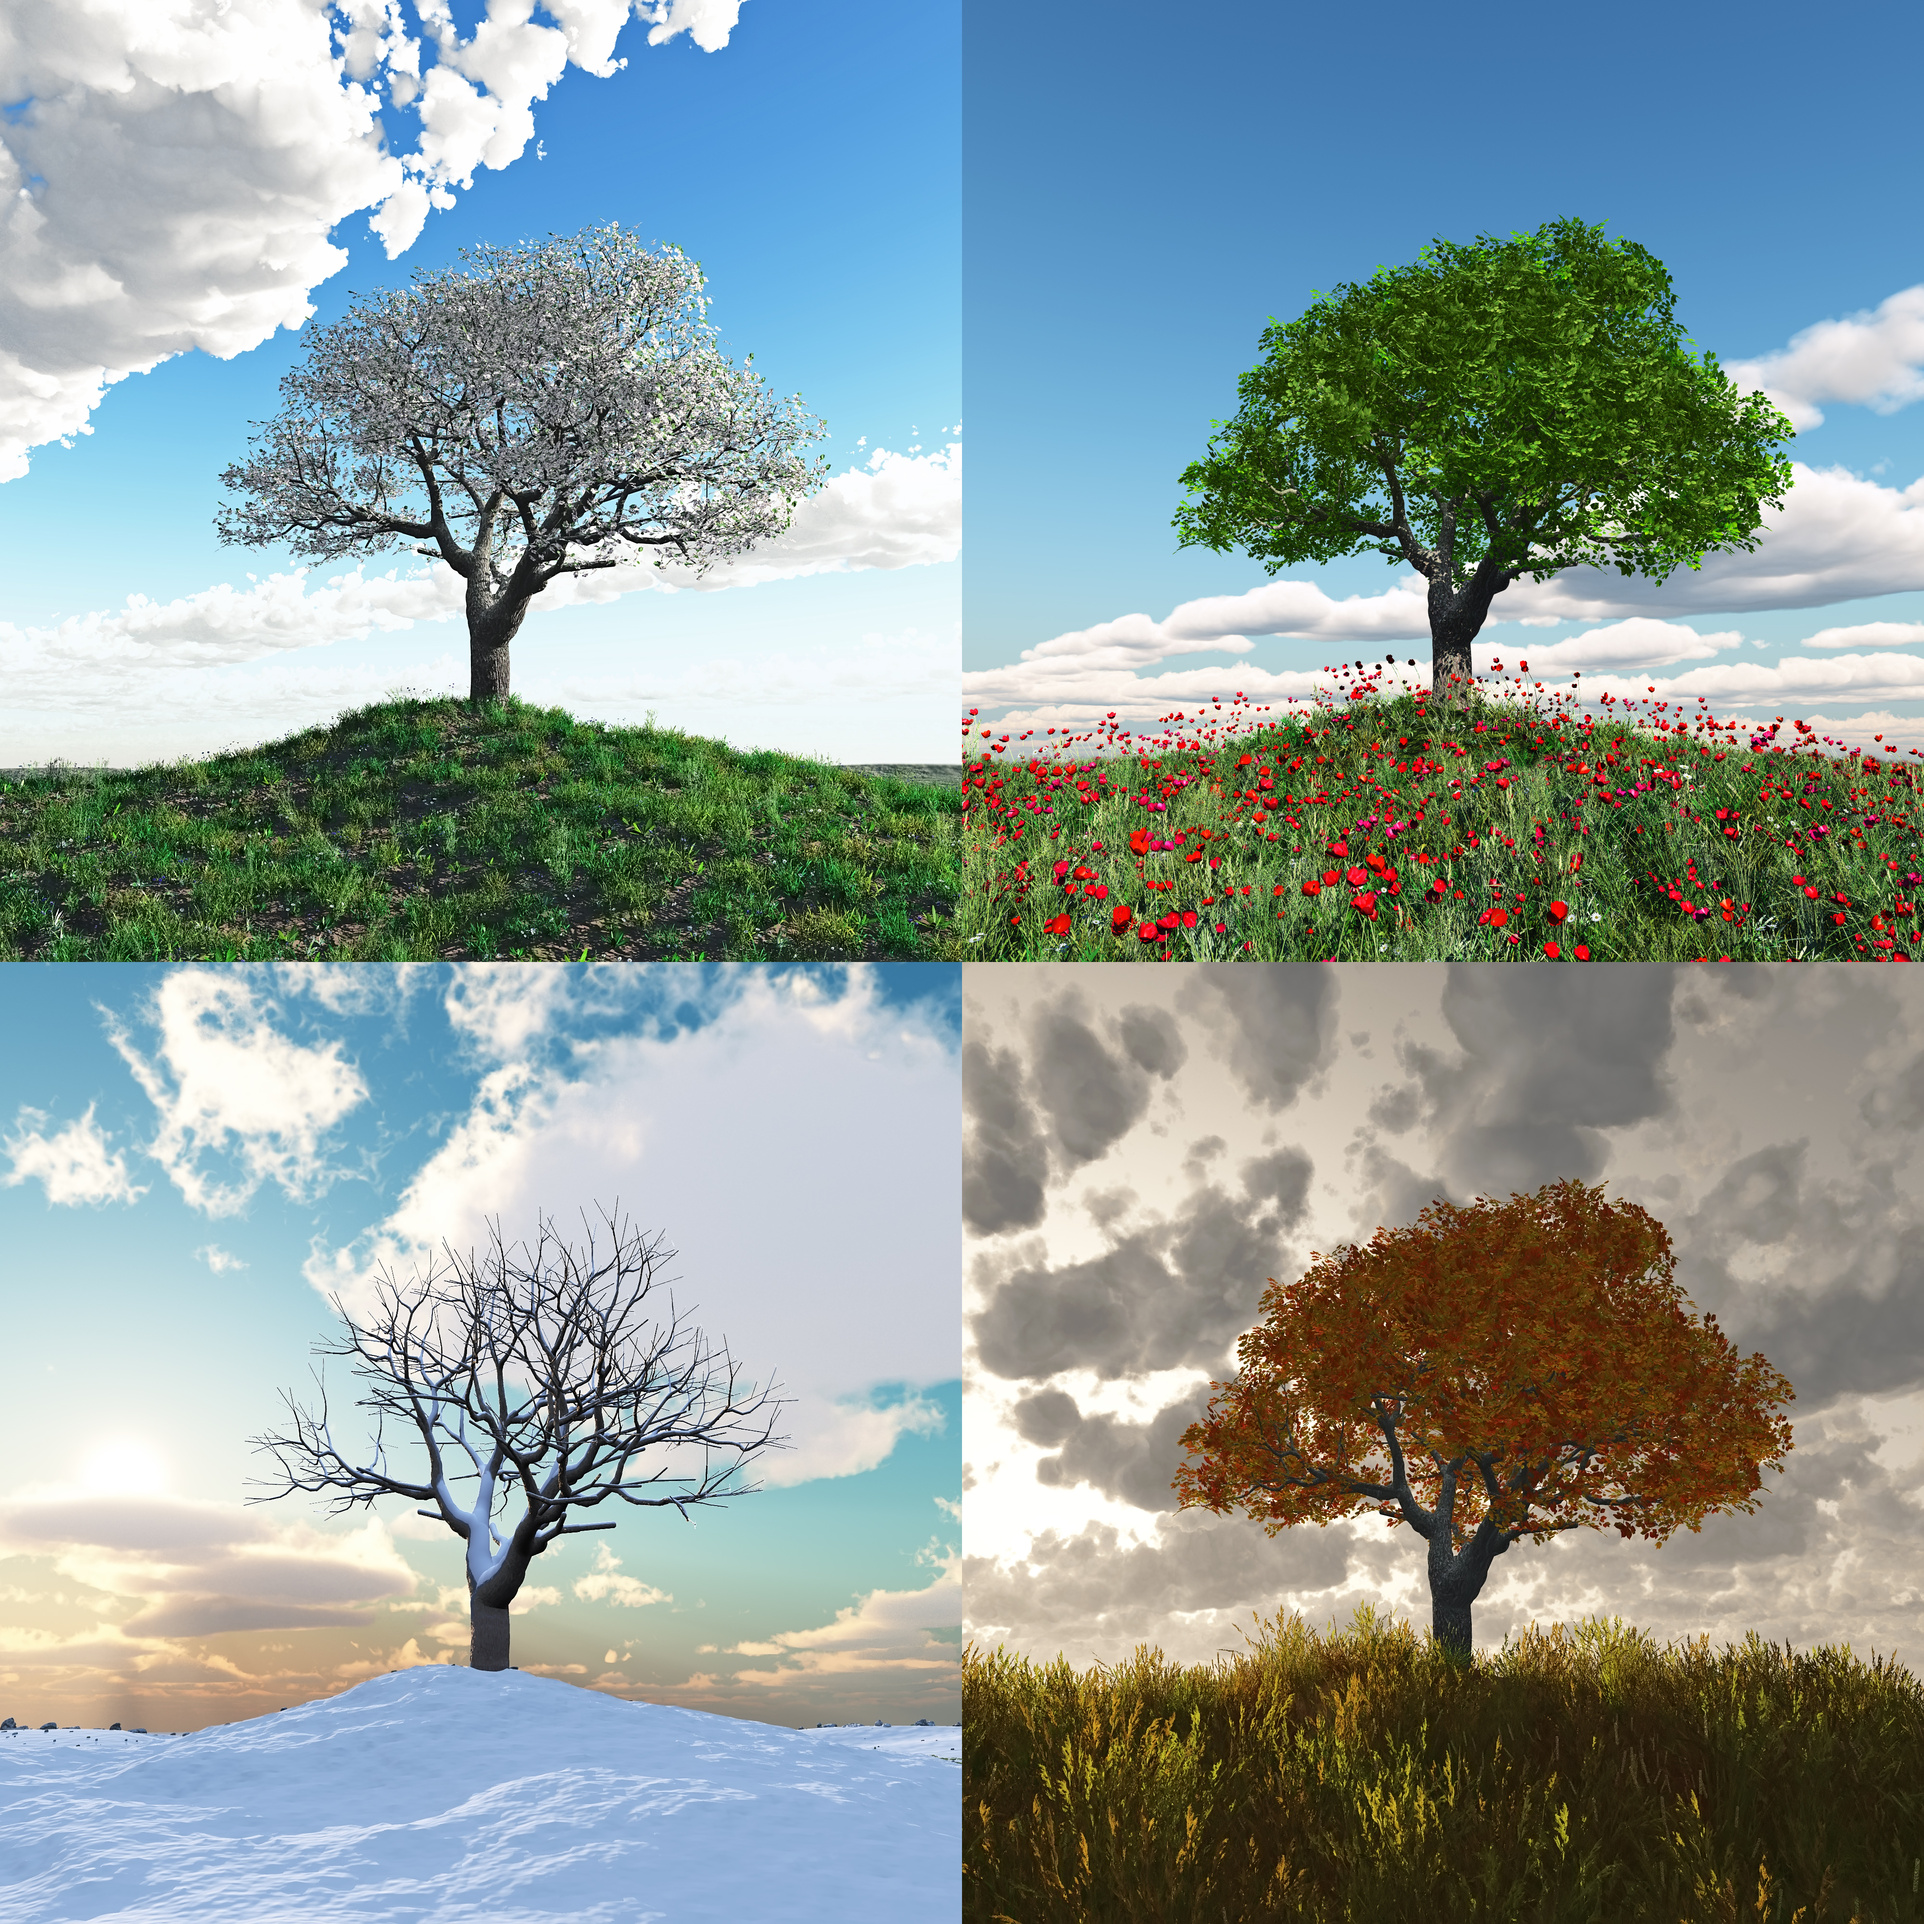
\includegraphics[width=0.5\linewidth]{quatre-saisons.jpg}
    \caption{les 4 saisons.}
    \label{fig:enter-label-1}
\end{figure}

\end{frame}


\begin{frame}{Principe}
\framesubtitle{Comment la prévision est faite?}

\begin{itemize}
    \item Calculer l'anomalie du modèle.
    \item déterminer les quantiles (1/3 , 2/3).
    \item projeter les ensembles.
\end{itemize}
\end{frame}

\begin{frame}{Principe}
\framesubtitle{Comment la prévision est faite?}
\begin{figure}
    \centering
    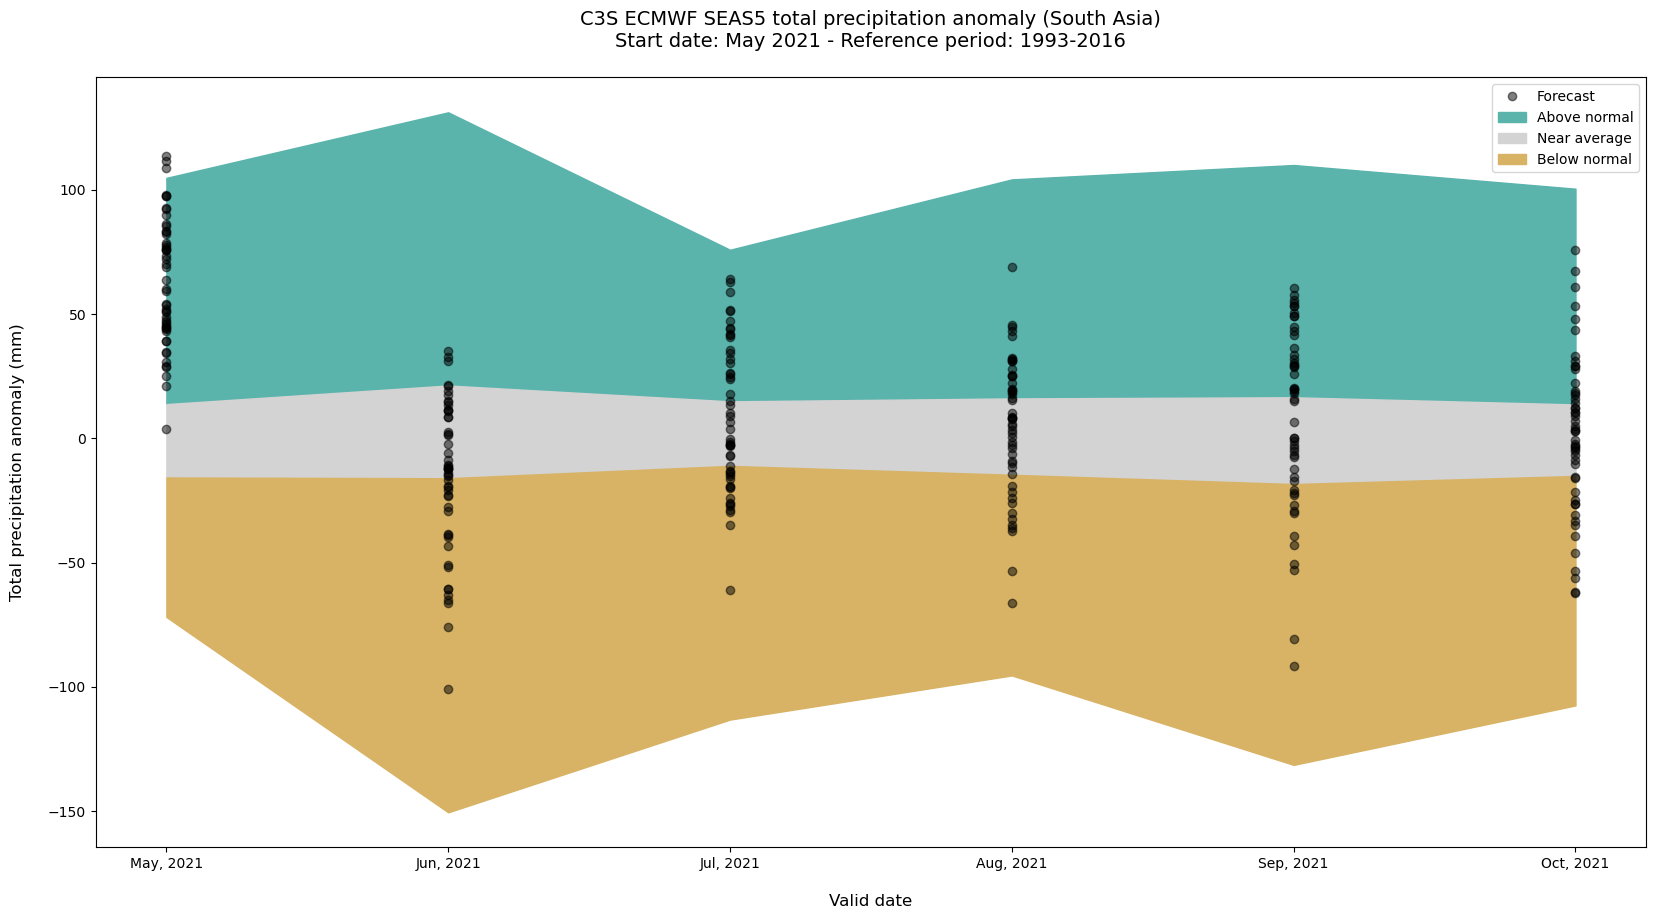
\includegraphics[width=0.8\linewidth]{sf_ensemble.png}
    \caption{Precipitation Forecast}
    \label{fig:enter-label}
\end{figure}
    
\end{frame} 
%\chapter{Results}
\chapter{Results}
This chapter presents the results of our study, divided into two main sections: temperatures and precipitation. In each section, we provide a comprehensive analysis of the deterministic and probabilistic evaluation of forecast performance across the MENA region. By examining both temperature and precipitation metrics, we aim to highlight the strengths and limitations of the forecasting models, offering valuable insights into their reliability and applicability in this climatically diverse area.
\section{Temperature}

In the temperature session, the use of heatmaps and temperature metrics maps will allow for a visual interpretation of model performance across various metrics. By analyzing these heatmaps, we can identify the most effective models based on metrics such as Spearman rank correlation, RMSE (Root Mean Square Error), and the Coefficient of Determination (R-squared). These visualizations will help in understanding the relationships between predicted and observed temperatures, aiding in the selection of models with the highest predictive accuracy. Additionally, the use of probabilistic evaluation metrics such as the Brier Score, Reliability, Ranked Probability Score (RPS), and Relative Operating Characteristics (ROC) will provide insights into the model's performance in terms of forecast quality, focusing on calibration, discrimination, and sharpness. These methods will be used to refine and improve predictive models for temperature forecasting in the MENA region.
\subsection{Deterministic evaluation results}

\subsubsection{ACC}

\begin{figure}[H]
	\centering
	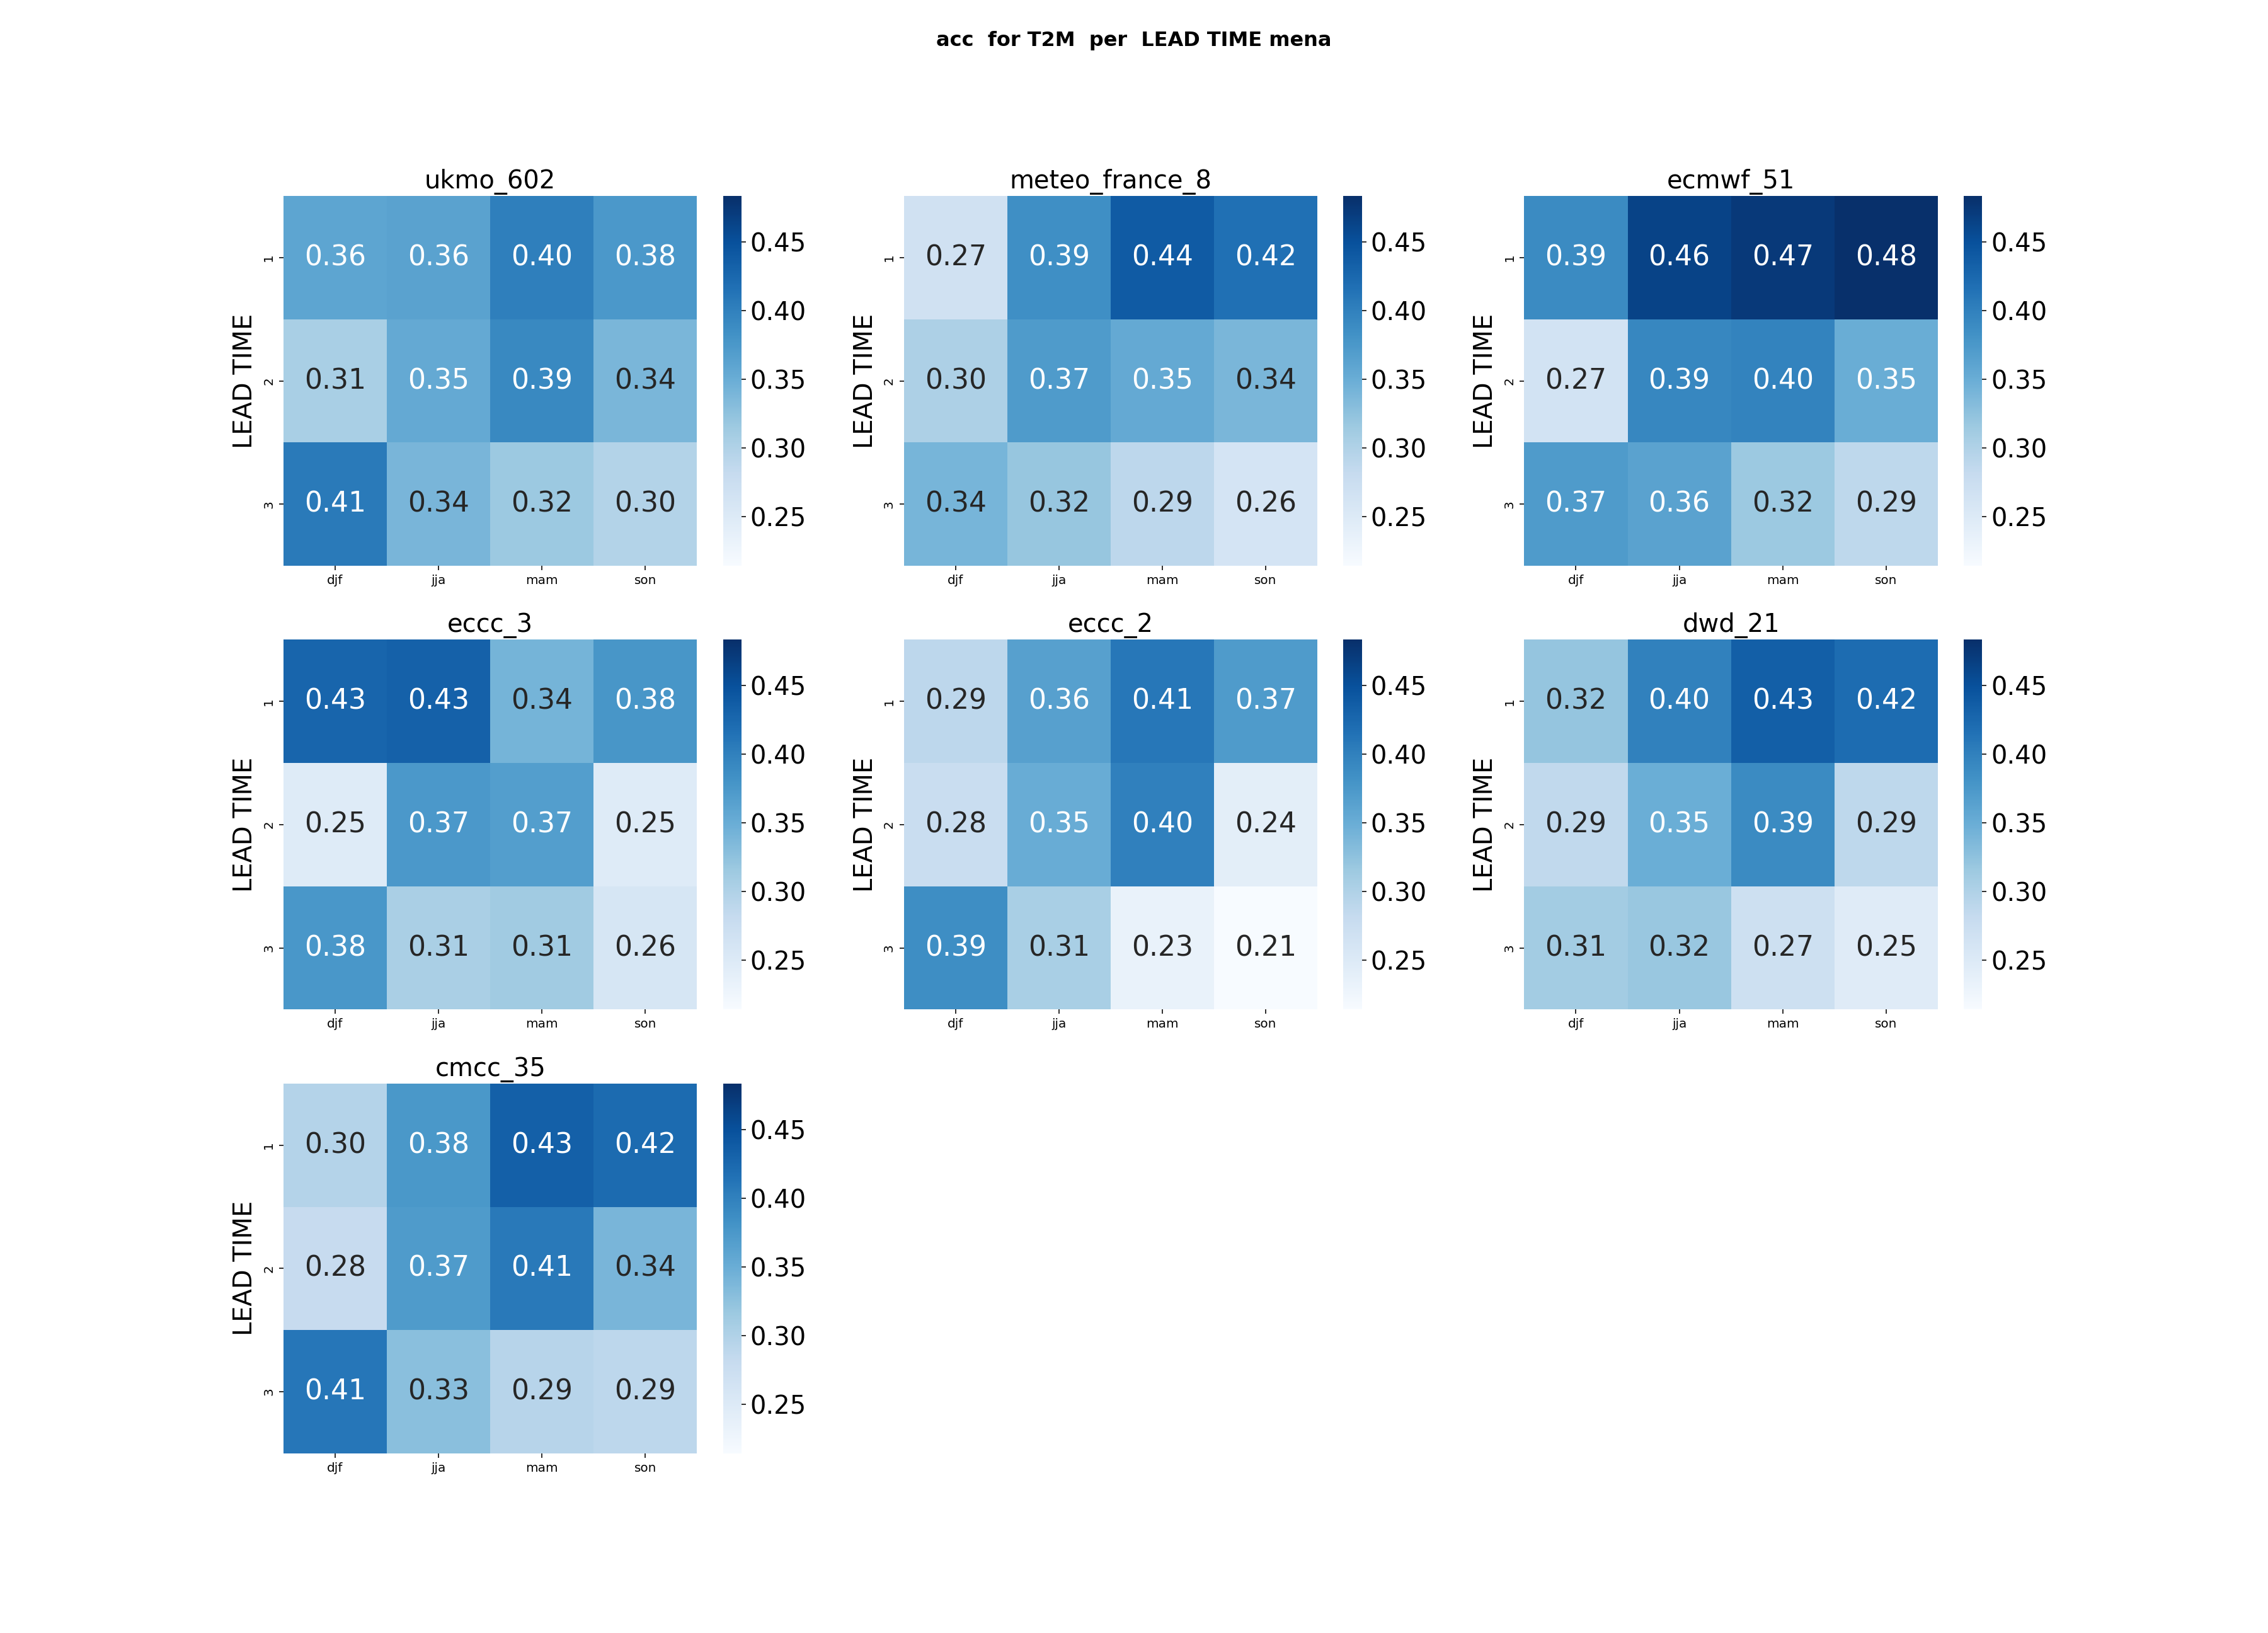
\includegraphics[scale=0.25]{plots/det/acc/acc_T2M_mena.png}
	\caption{The Heatmap of acc for the mena region for every period \textbf{\textit{(1 for perfect Correlation)} }}
\end{figure}
The acc is moderate for all centers; however, the best models are \textbf{\textit{ECMWF, meteo-france and eccc-3}}. There is no clear variability in performance over time. For SON and JJA, performance is good at time 1 for all centers but decreases with increasing lead-time..



\subsubsection{Root Mean Square Error}


The maps in this section show the RMSE (Root Mean Square Error) between observed and modeled surface temperatures across the MENA region for the four seasons: JJA, DJF, MAM, and SON. The RMSE, expressed in the same units as temperature, evaluates the accuracy of climate models, with lower values indicating better performance.  These maps help identify the strengths and limitations of the models across seasons, contributing to the improvement of climate forecasts for the region.
\begin{figure}[H]
    \centering
    \includegraphics[width=1\linewidth]{plots/det/rmse/rmse_T2M.png}
    \caption{Temperature rmse heatmaps for all the sasons}
    \label{fig:CORR_djf_t2m}
\end{figure}

The heatmap for the seven models highlights distinct variations in their seasonal performance. The UKMO model shows moderate to good performance, particularly in JJA and MAM, as reflected by relatively low RMSE values ranging between 1.35°C and 1.51°C across the three lead times. This indicates that the UKMO model is reasonably effective in capturing surface temperature variations during these seasons, likely benefiting from its ability to simulate key atmospheric processes during these periods.

In contrast, Météo-France exhibits weaker performance in JJA, with higher RMSE values suggesting less accurate predictions of surface temperatures during this season. This could be attributed to the model's limitations in capturing summer-specific temperature drivers in the MENA region, such as heatwaves, desert-air interactions, or seasonal atmospheric circulation patterns.

The ECMWF model emerges as the best-performing model based on the heatmap, particularly during JJA, where it demonstrates high predictive accuracy and consistency. This is supported by the RMSE map, which shows significantly lower RMSE values across most of the MENA region. These low RMSE values confirm the ECMWF model's ability to capture regional temperature dynamics effectively, with reduced errors across diverse climatic zones.

Notably, the spatial distribution of RMSE on the map reinforces the ECMWF's strong performance, as it maintains relatively low error values in critical parts of the MENA region. This suggests that the ECMWF model is better equipped to account for the complex climatic interactions in the region, such as the influence of desert regions, coastal temperature gradients, and seasonal weather patterns.

Overall, these findings emphasize the importance of selecting climate models based on their seasonal and spatial performance, as they play a critical role in improving the accuracy of temperature forecasts for the MENA region.







\subsubsection{coefficient of determination}


The maps in this section show the Rsquared between observed and modeled surface temperatures across the MENA region for the four seasons: JJA, DJF, MAM, and SON. R-squared is a statistical measure that indicates how well the model explains the variability in observed data, with values closer to 1 signifying better performance. These maps provide valuable insights into the predictive skill of the climate models, highlighting their ability to capture seasonal temperature patterns.

\begin{figure}[H]
    \centering
    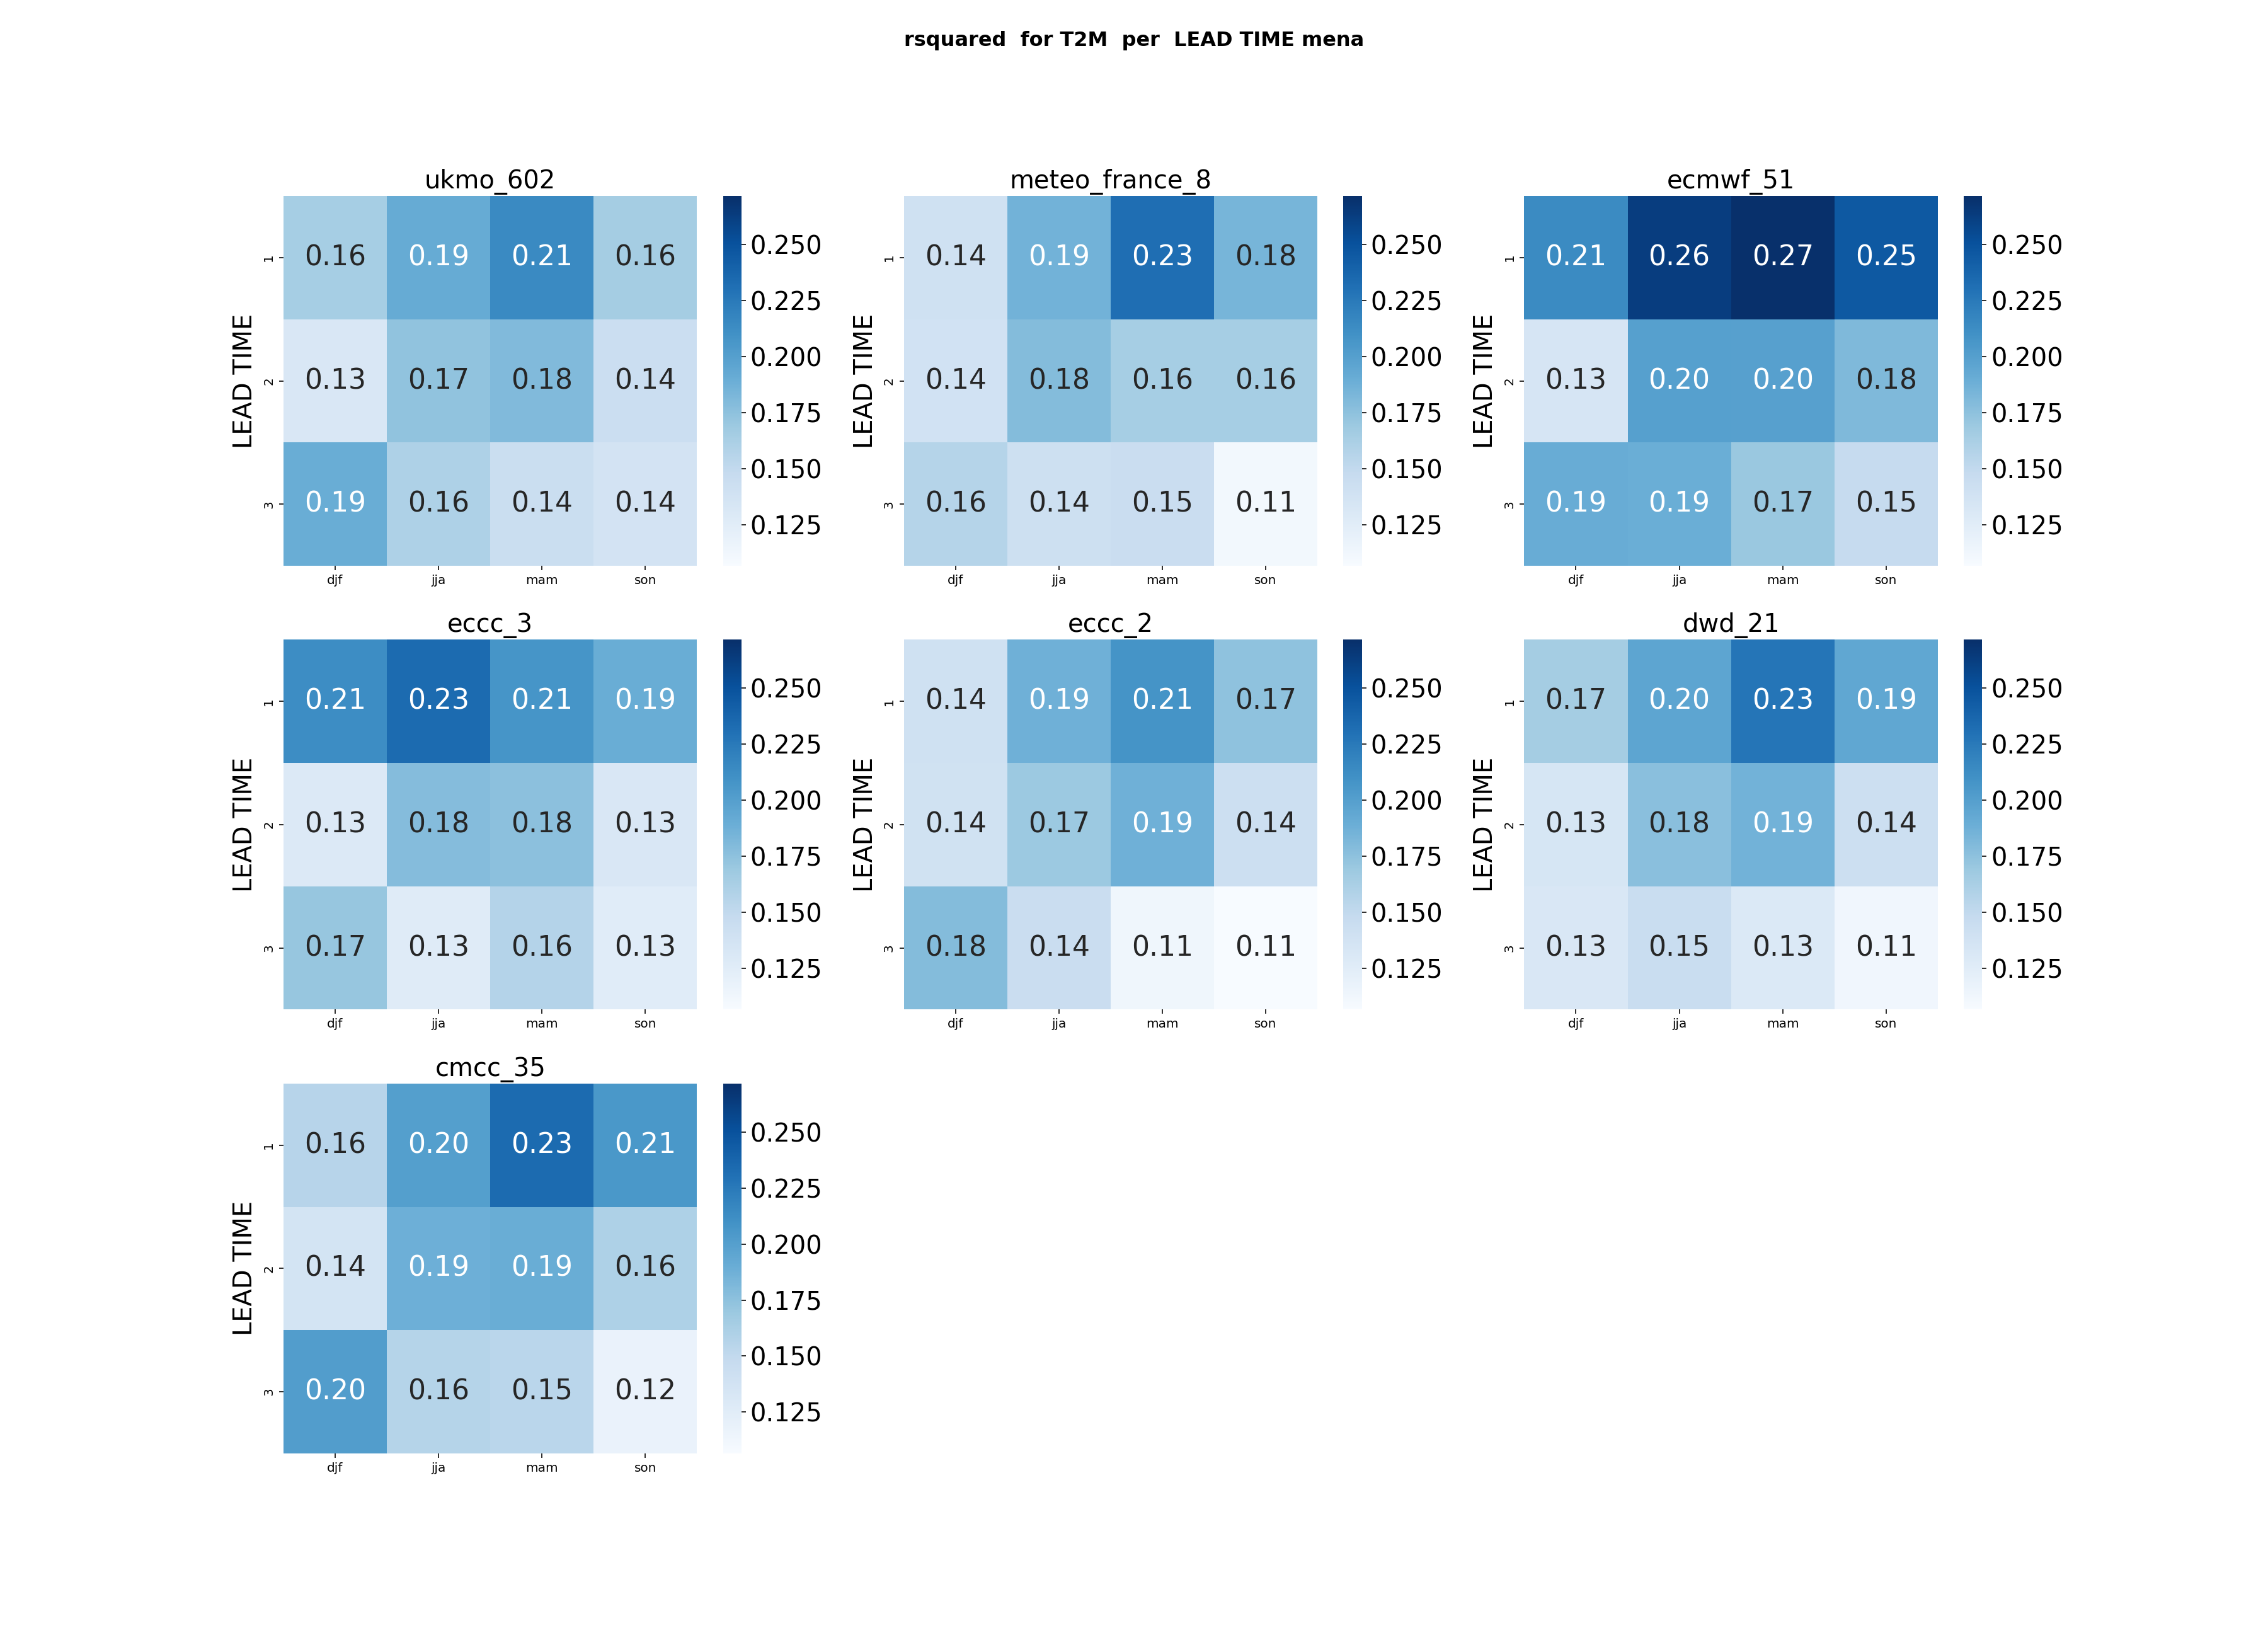
\includegraphics[width=1\linewidth]{plots/det/rsquared/rsquared_T2M_mena.png}
    \caption{Temperature rsquared heatmaps for all the seasons}
    \label{fig:CORR_djf_t2m}
\end{figure}
Based on this deterministic metric (R-squared), the ECMWF model demonstrates superior performance for lead time 1 across all four seasons, particularly during MAM. In general, the portion of variance explained by the model decreases as the lead time increases. This indicates that while the model is highly effective at capturing seasonal variability of surface temperatures in the short term, its predictive skill diminishes over longer time horizons.

The strong performance during MAM highlights the ECMWF model’s ability to capture the complexities of spring, a season marked by transitional weather patterns in the MENA region. The high R-squared values during this period suggest that the model accurately reflects observed temperature variability by effectively simulating key drivers such as the gradual warming trend, atmospheric circulation changes, and the interaction between desert and coastal dynamics.

Such precision underscores the ECMWF model’s reliability for short-term seasonal forecasting, particularly during periods of heightened climatic variability like MAM. However, the decreasing performance with increasing lead times suggests the need for careful interpretation of forecasts beyond lead time 1, as uncertainty increases with longer projections.

\begin{figure}[H]
    \centering
    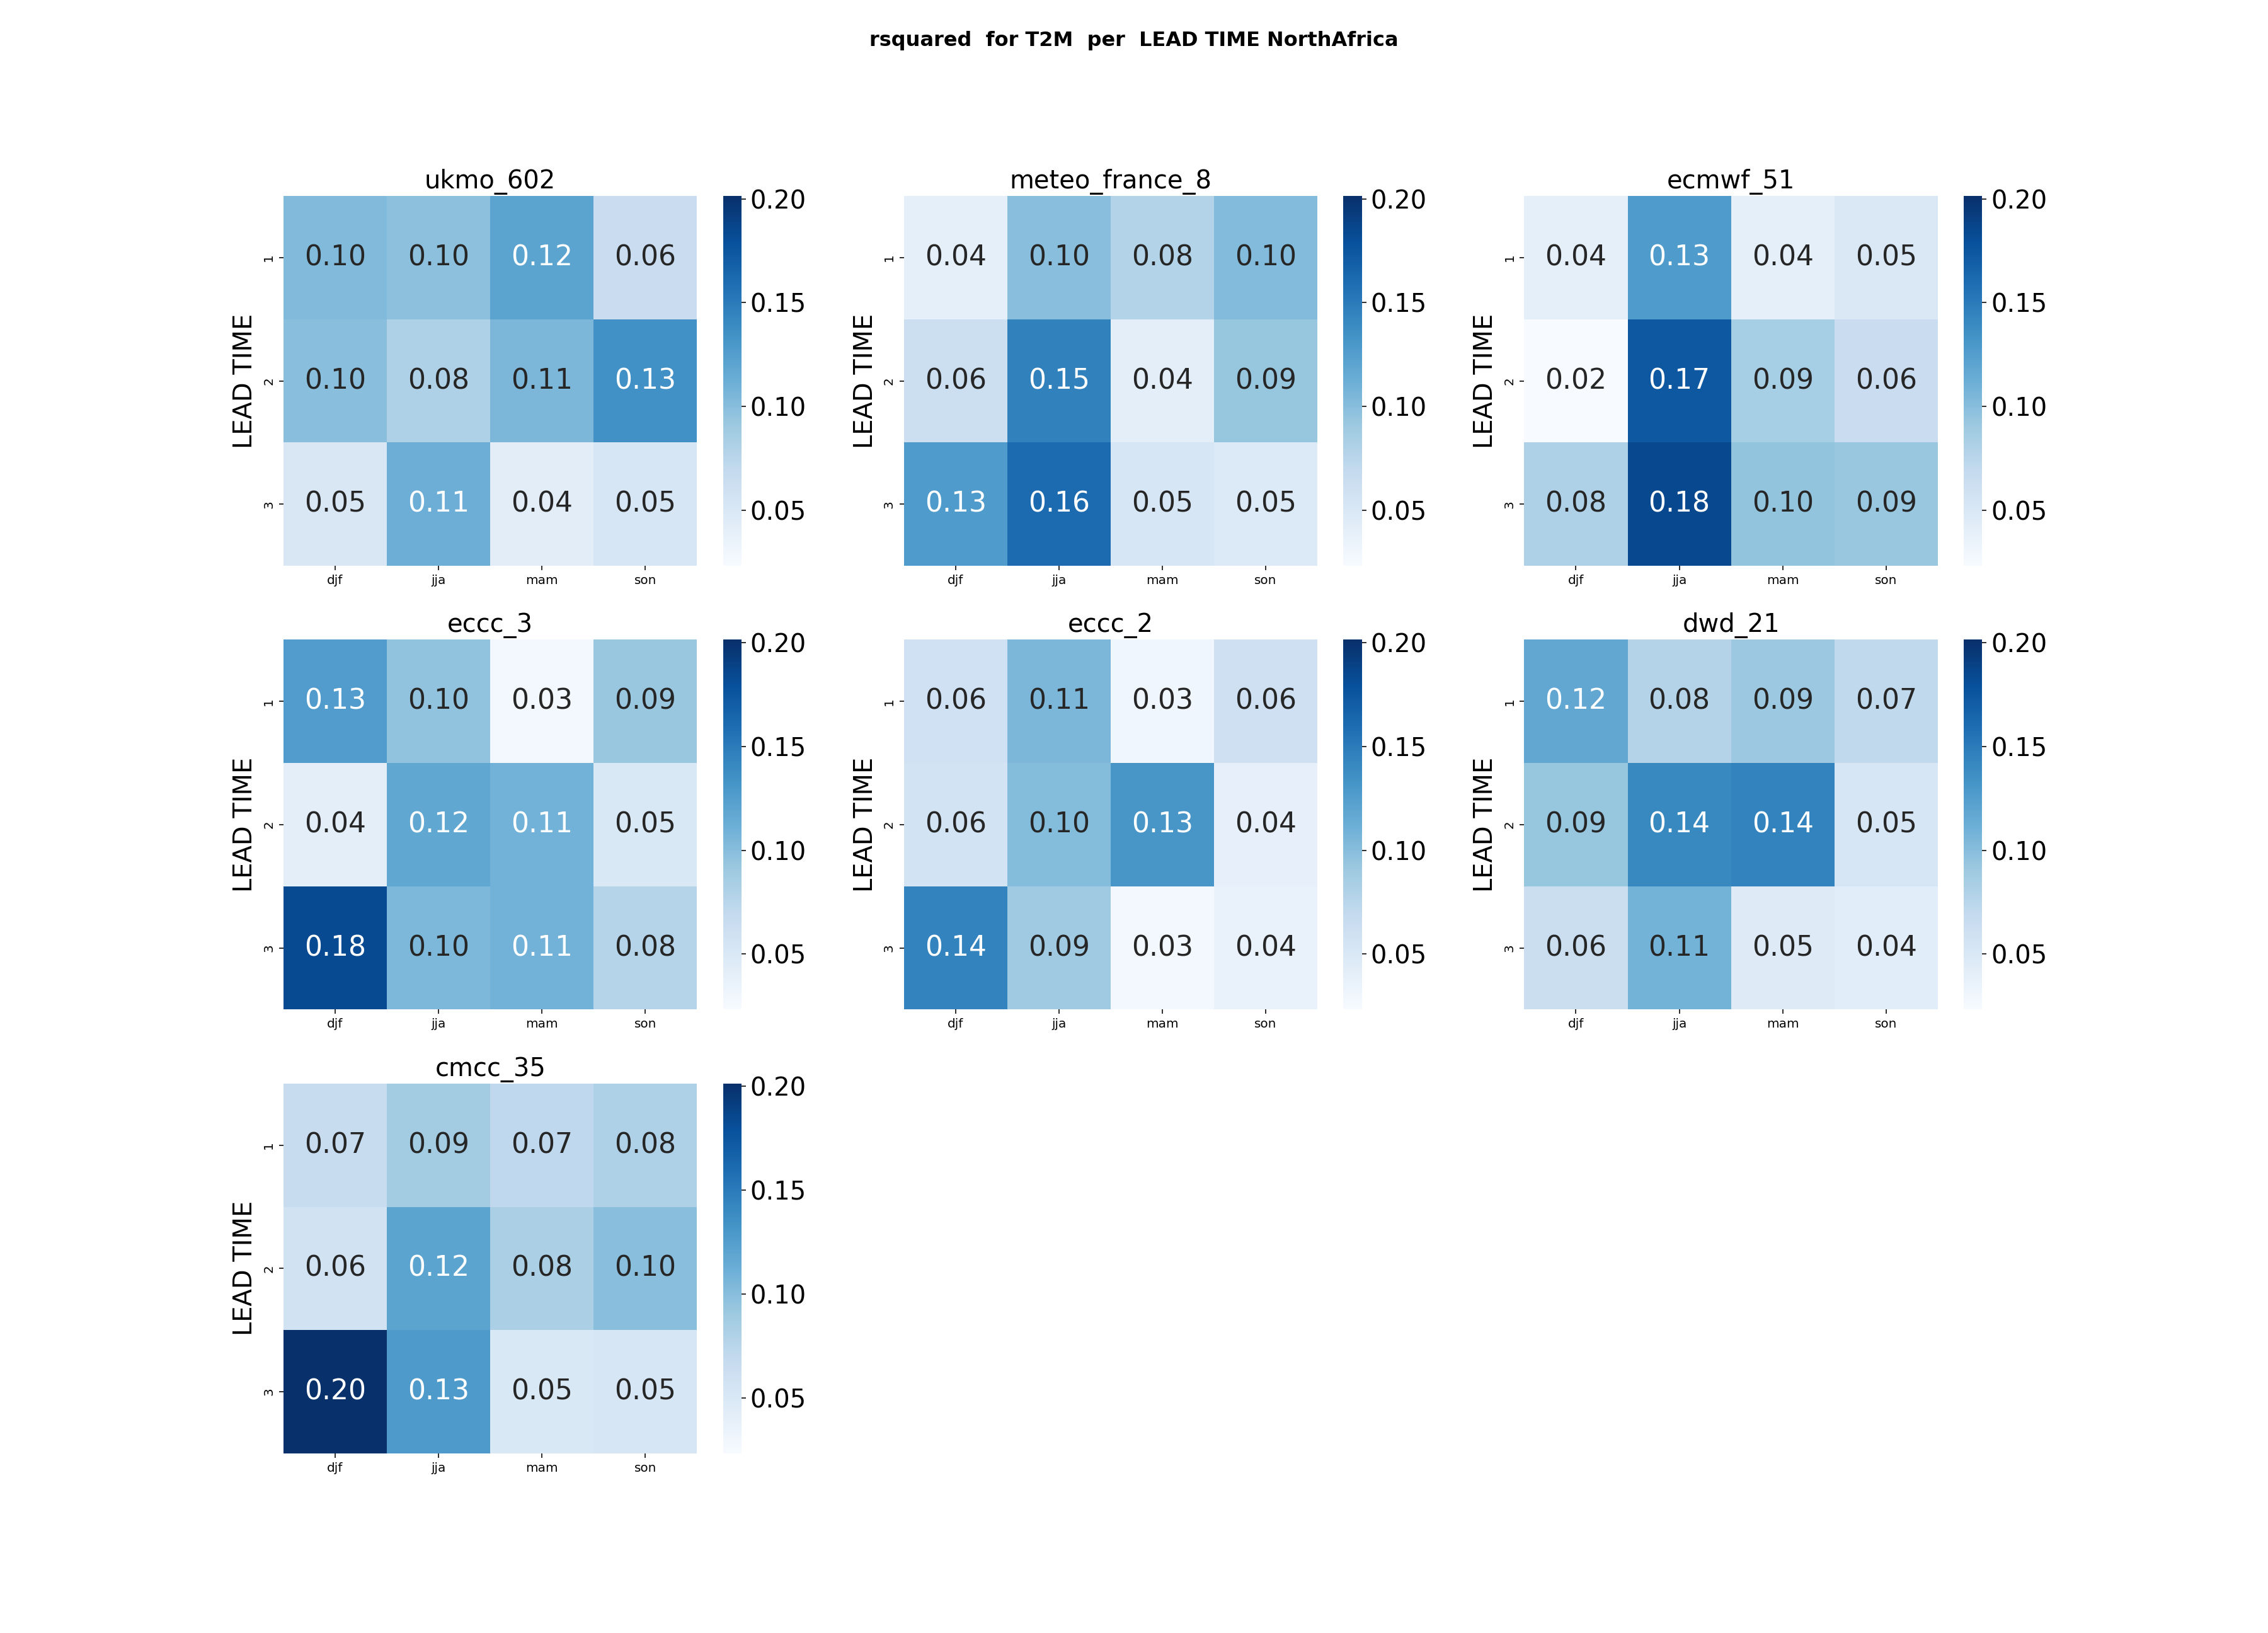
\includegraphics[width=1\linewidth]{plots/det/rsquared/rsquared_T2M_NorthAfrica.png}
    \caption{Temperature rsquared heatmaps for all the seasons}
    \label{fig:CORR_djf_t2m}
\end{figure}
A closer look at North Africa reveals that the ECMWF model performs best during JJA, with R-squared values increasing as the lead time increases—contrary to the trend observed for the MENA region as a whole, where performance typically decreases with longer lead times. This suggests that the ECMWF model is particularly adept at capturing the persistent summer temperature patterns in North Africa, which may benefit from stronger model predictability over time due to the relatively stable atmospheric and climatic conditions during JJA.

Similarly, Météo-France also shows good performance in North Africa, maintaining consistent R-squared values across different lead times and seasons. This consistency highlights the model’s ability to handle the diverse climatic features of the region, such as the extreme temperatures influenced by the Sahara Desert and the moderating effects of the Mediterranean coastline.

These findings emphasize the importance of regional analysis, as the performance of climate models can vary significantly within sub-regions of MENA. While ECMWF excels in predicting North Africa’s summer temperatures, the observed increase in R-squared with lead time underscores the need to investigate the underlying factors driving this unusual trend, which contrasts with the broader MENA region’s dynamics.



\subsection{Probabilistic evaluation results}

To complement the deterministic evaluation of model performance, probabilistic evaluation metrics are employed to assess the reliability and skill of climate models in predicting the likelihood of specific outcomes. Unlike deterministic metrics, which focus on the accuracy of single-point predictions, probabilistic metrics evaluate the quality of the models’ forecast distributions, accounting for uncertainty and variability in predictions. These metrics are essential for understanding how well models represent the range of possible outcomes, particularly in regions like MENA, where climatic variability and extremes are prominent. By incorporating probabilistic metrics, this analysis provides a more comprehensive evaluation of the models’ predictive capabilities and their usefulness in decision-making under uncertainty.
The figures illustrate two main approaches to probabilistic assessment metrics, including the Brier Score (BS) and others. The first approach averages across lead times and grid points, while preserving categories, where the final figure contains the value of the metric for each season across all four seasons, for each category (mean, lower, upper) defined by the 1/3 quartiles. This method provides insight into the predictive ability of models under different seasonal conditions and forecast probability categories, particularly how well models capture temperature variations in the middle, lower, and upper quartiles of the predicted probability distribution. The diversity of metric values ​​across these categories helps highlight the sensitivity of models to different levels of forecast confidence. It indicates their ability to differentiate between forecast uncertainty and actual observed outcomes, providing a nuanced understanding of how accurately models predict different temperature ranges.

The second approach averages all grid points in the MENA region while retaining all lead times and seasons. This aggregated view provides an overall assessment of the measure for each season, considering all lead times and forecast categories. This approach focuses on how models perform across different forecast scenarios and how well they produce accurate and reliable temperature forecasts, regardless of forecast probability. By retaining lead times and seasons in the analysis, this method provides a comprehensive picture of model performance over time and under different climate conditions. It reveals how well models generalize across different forecast scenarios, helping to identify which models are most effective at producing consistent and reliable forecasts.
\subsubsection{Brier score}

The figure at the bottom illustrates that most models demonstrate relatively high performance, as indicated by a small Brier Score (BS), meaning that the predicted probabilities are close to the observed ones. This reflects accurate forecast probabilities forT2M The UKMO model, however, shows moderate performance with a larger BS, suggesting that its predicted probabilities are less closely aligned with observed outcomes compared to other models. Notably, the middle category presents lower performance relative to the other two categories (lower and upper). This indicates that while some models capture temperature variability well in extreme conditions (upper category), their skill diminishes when forecasting moderate changes (middle category). This discrepancy highlights the challenges models face in translating predicted probabilities into reliable forecasts, particularly for temperature variations that are neither extreme nor outlier events. 


\begin{figure}[H]
    \centering
    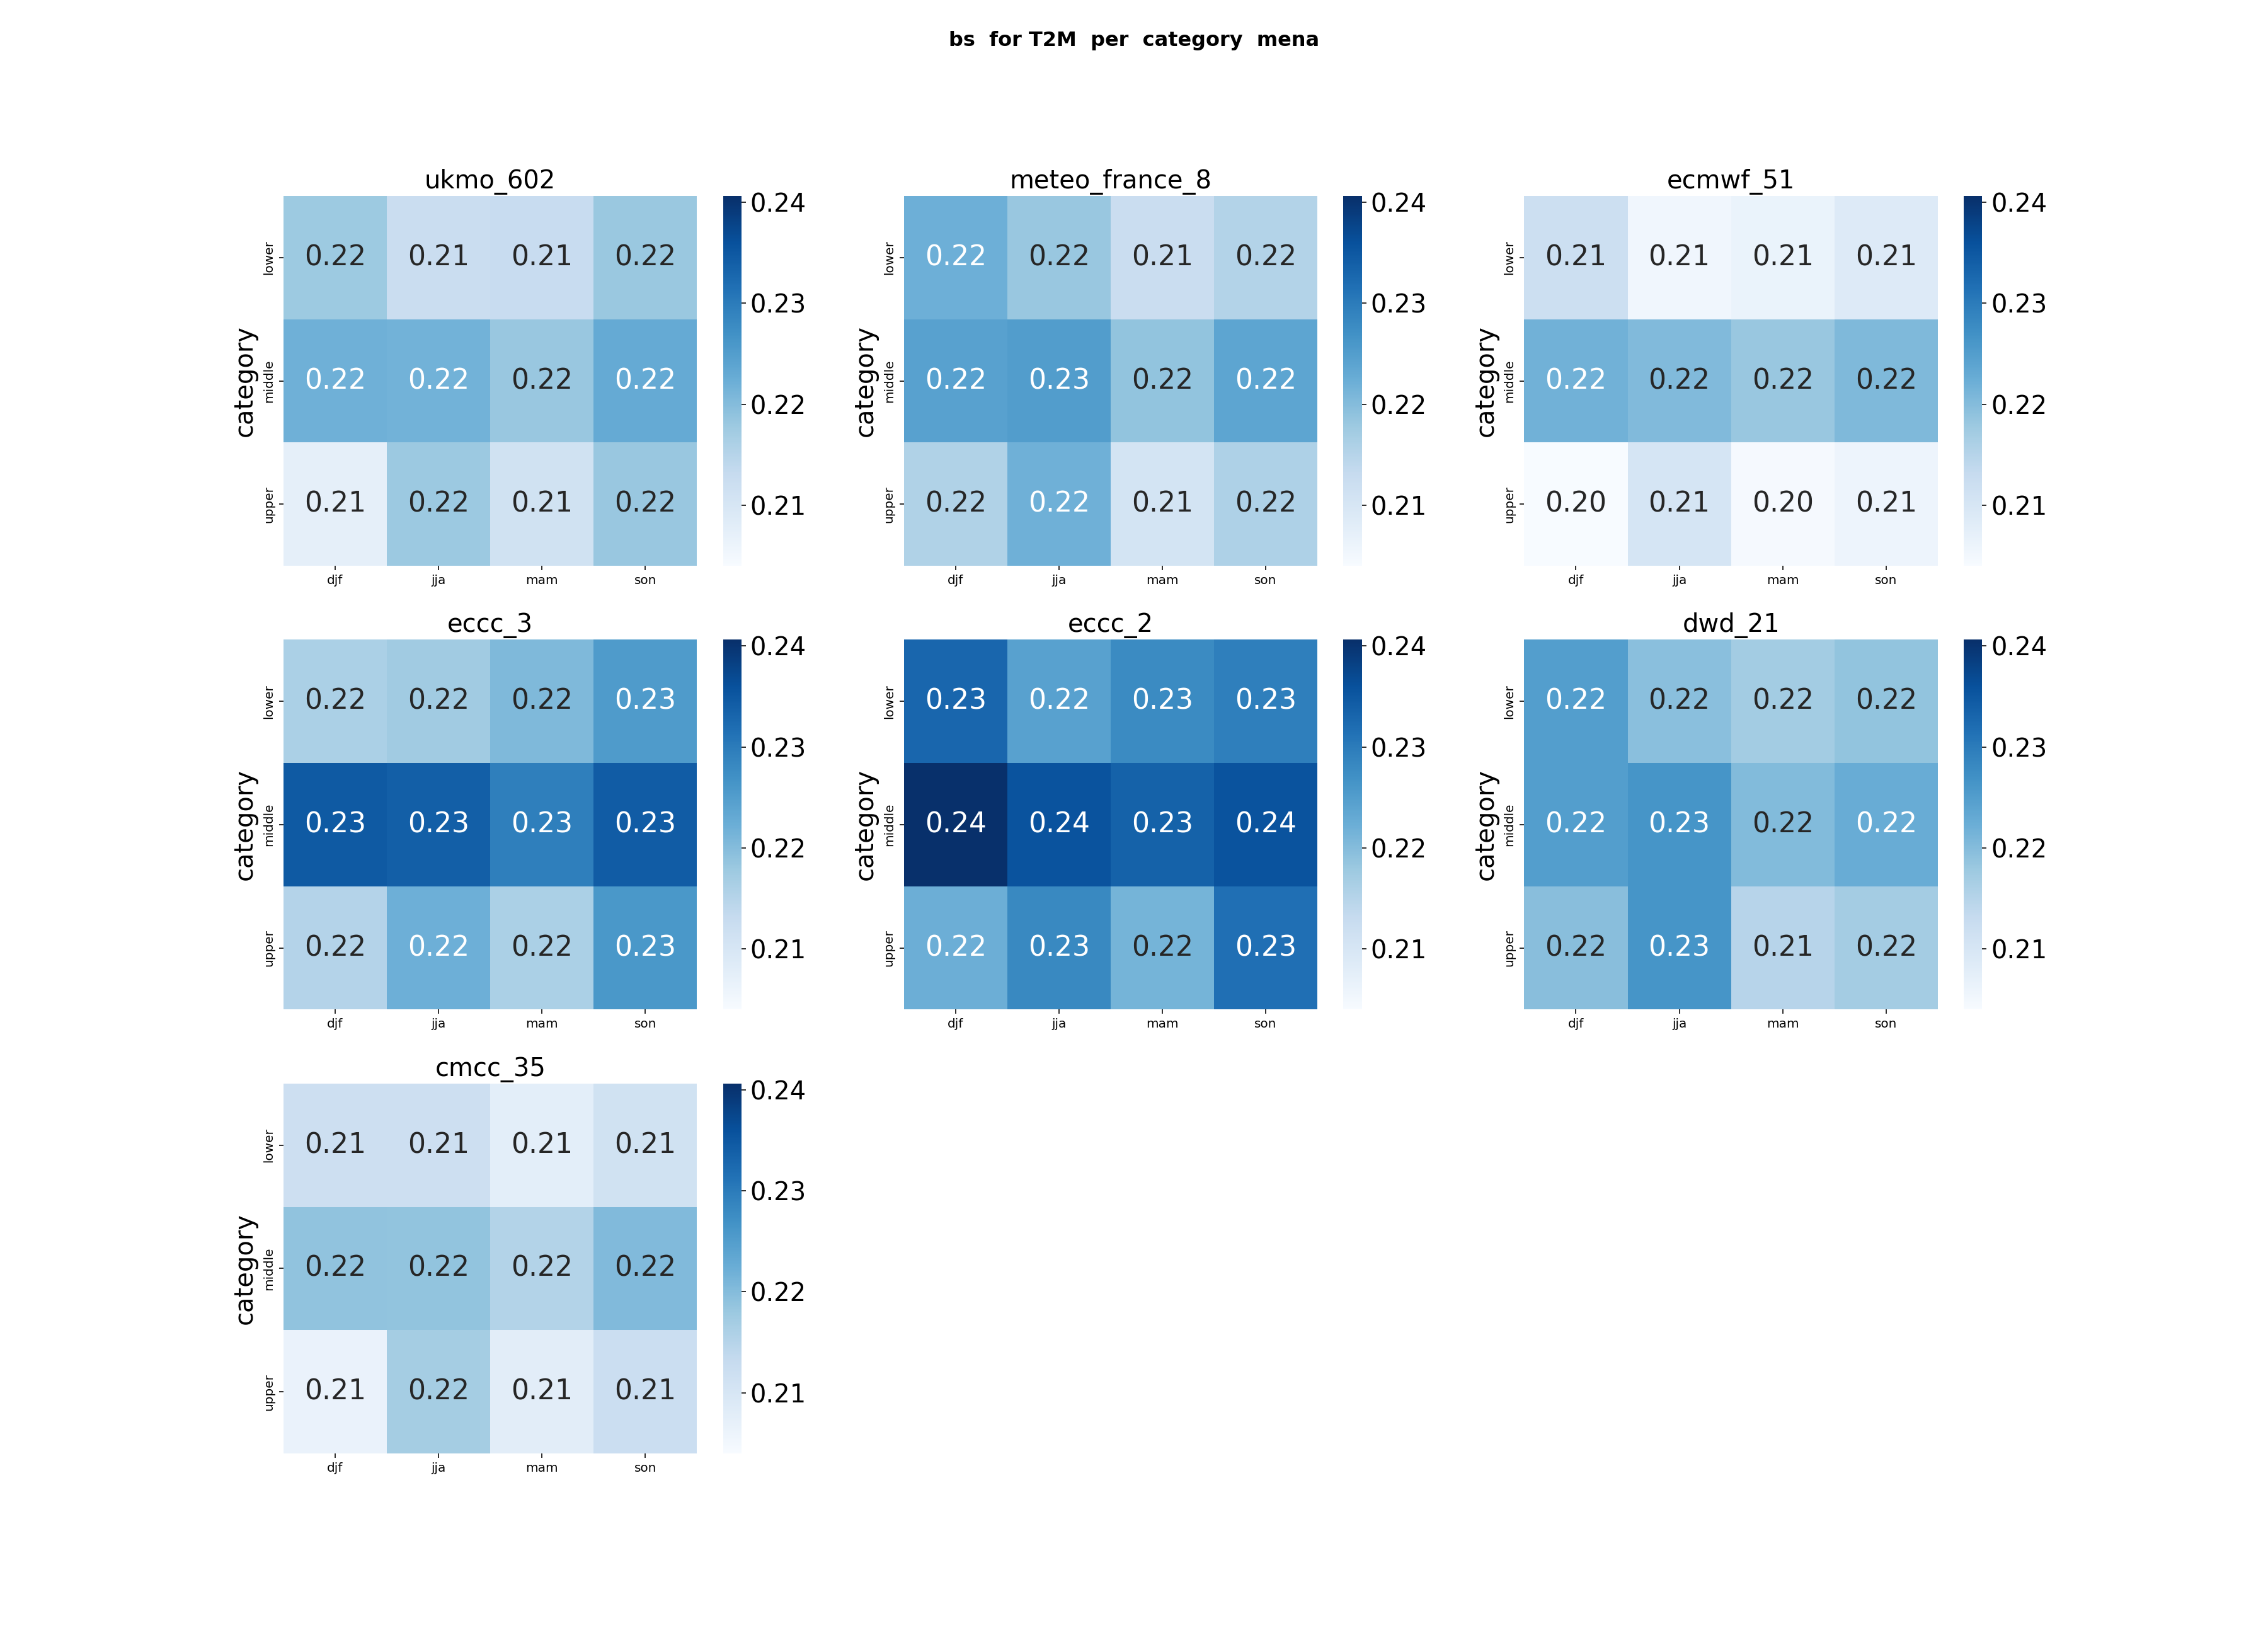
\includegraphics[width=1\linewidth]{plots/prob/bs/bs_T2M_category_mena.png}
    \caption{Temperature Brier score heatmaps for all the seasons per categories}
    \label{fig:CORR_djf_t2m}
\end{figure}
An analysis by lead time revealed that the models Meteo France, ECMWF, and CMCC exhibit superior performance, as indicated by lower Brier Scores (BS). This suggests that these models provide more accurate probabilistic forecasts for T2M compared to others. Moreover, the differences in BS values between successive lead times are minimal, indicating that the predictive skill of these models remains relatively consistent as the forecast horizon increases.

This stability in performance across lead times is particularly noteworthy, as it reflects the robustness of these models in maintaining their ability to produce reliable forecasts over time. The lower BS values also suggest that these models effectively capture the relationship between predicted probabilities and observed outcomes, ensuring high confidence in their probabilistic predictions. Such consistent performance across lead times is crucial for operational forecasting, as it highlights these models' reliability for both short- and medium-term forecasts in the MENA region.

\begin{figure}[H]
    \centering
    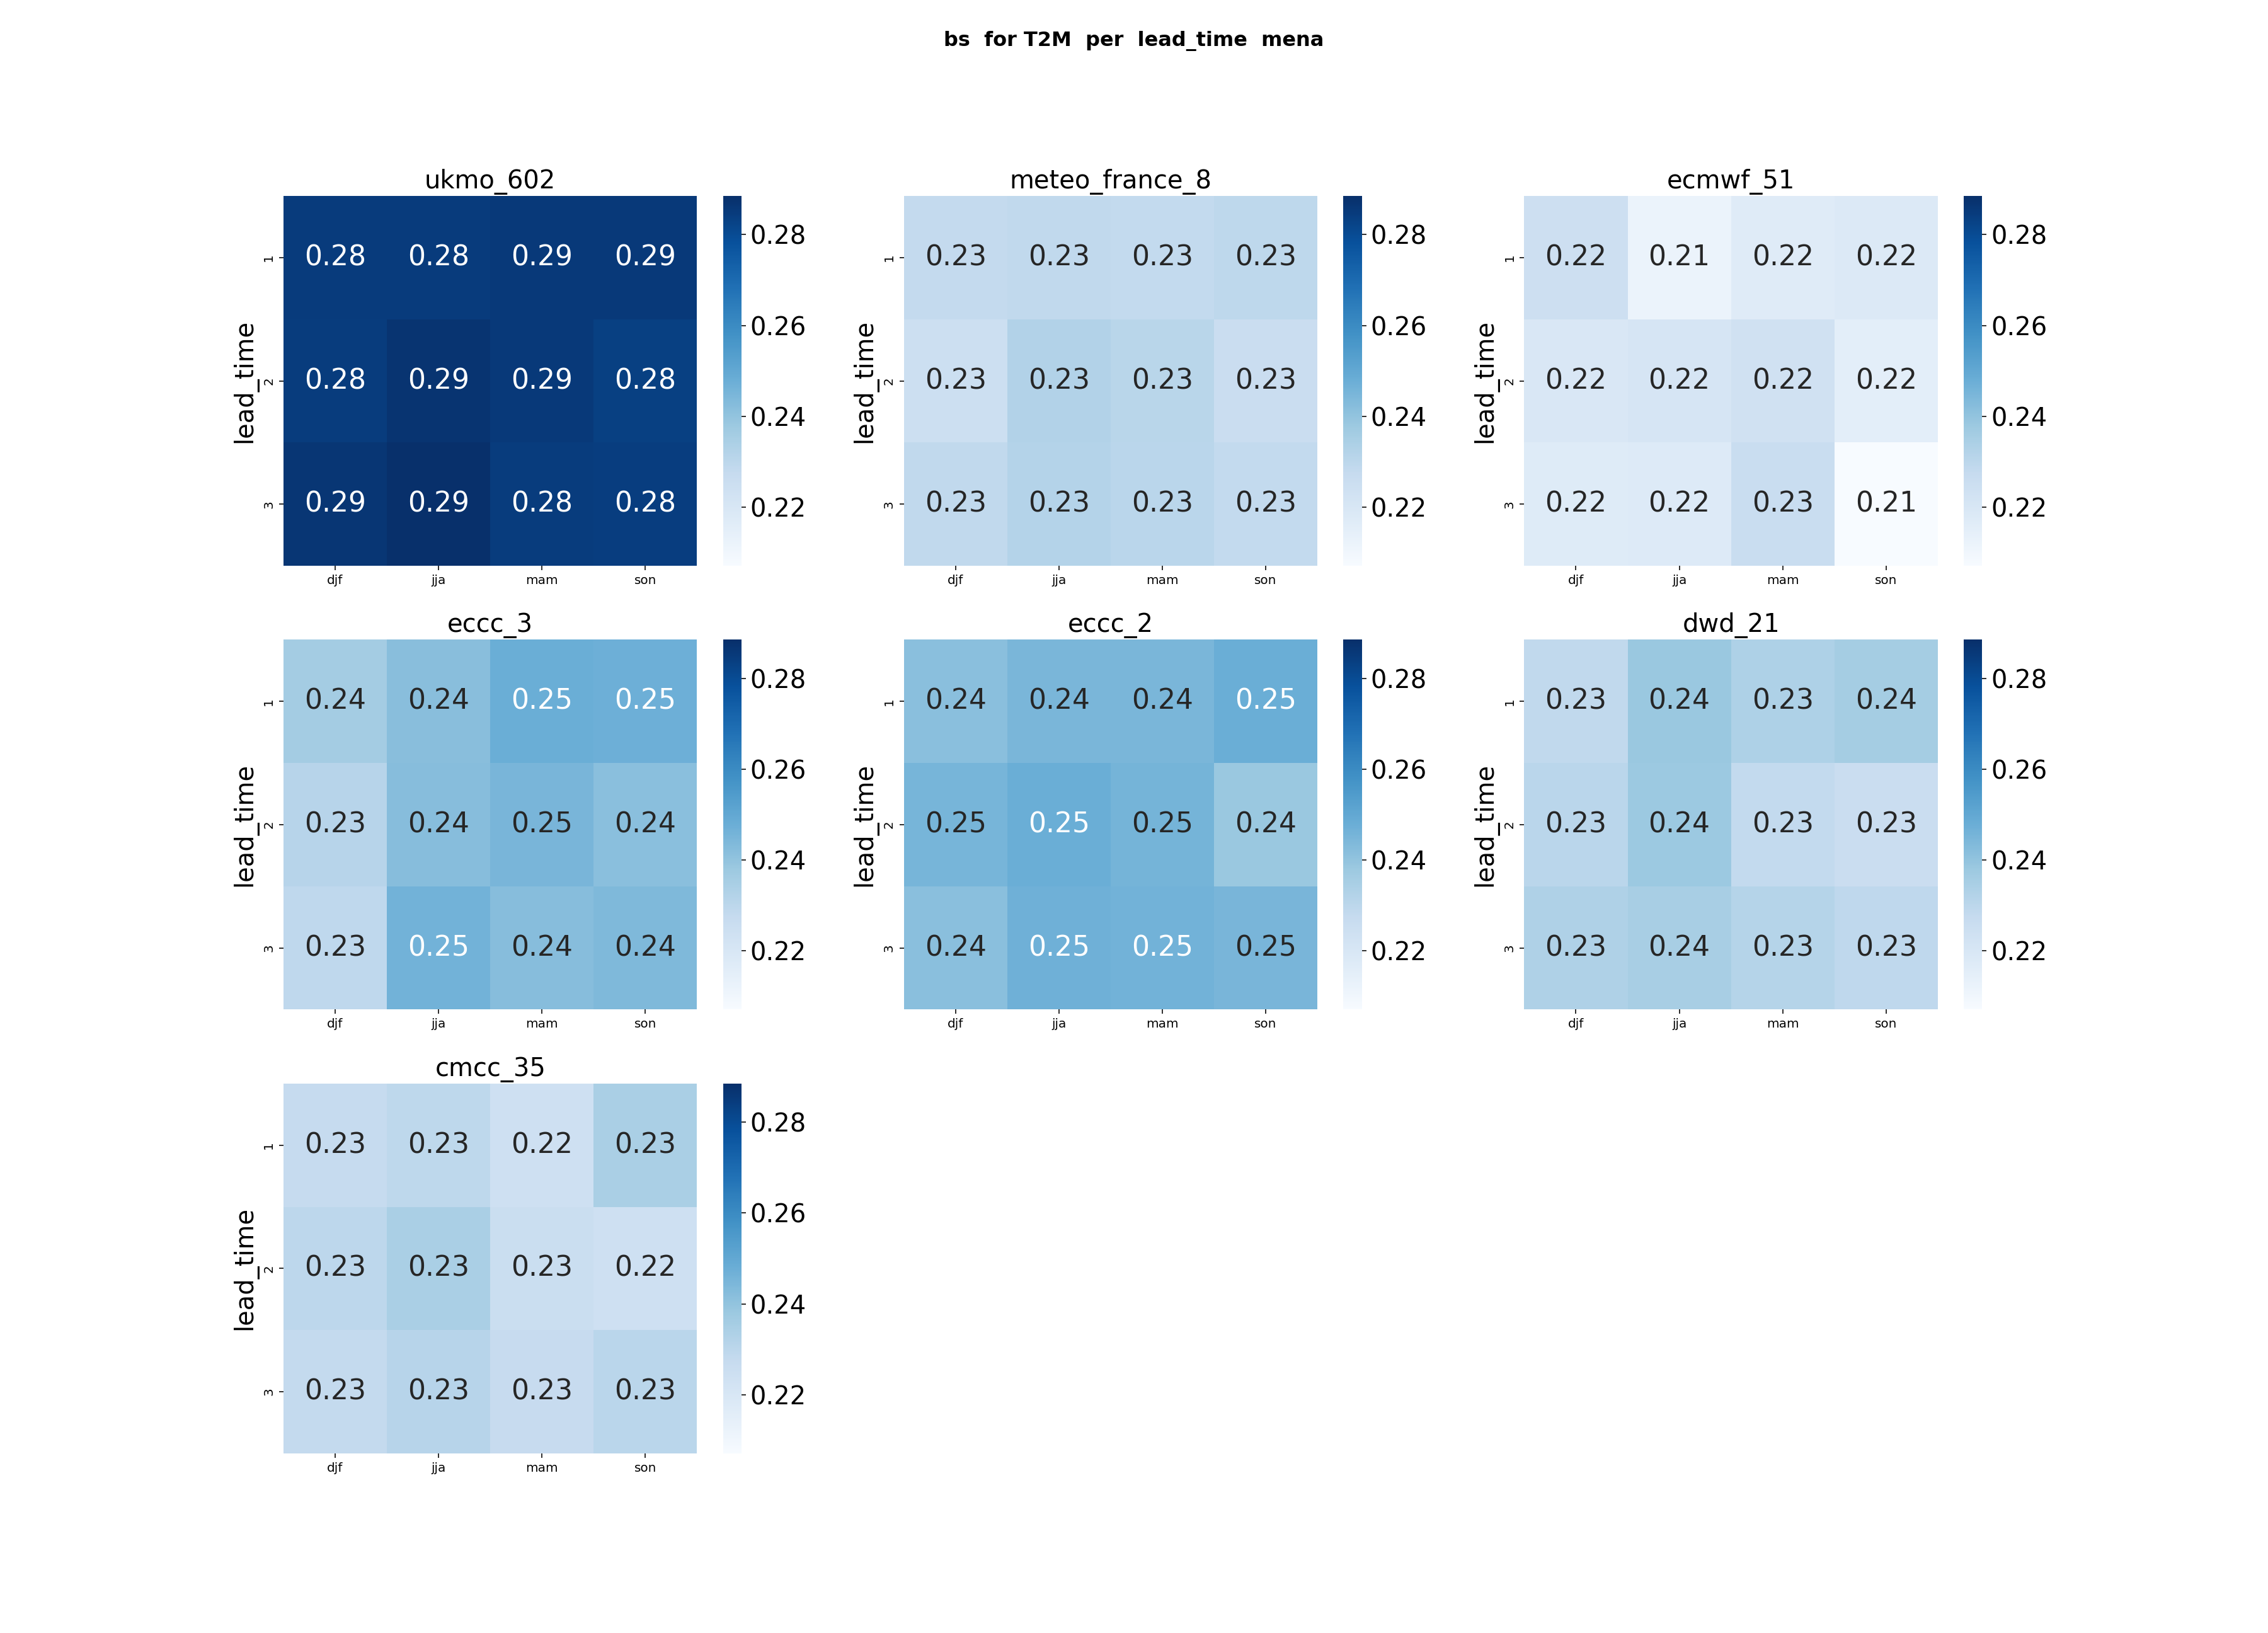
\includegraphics[width=1\linewidth]{plots/prob/bs/bs_T2M_lead_time_mena.png}
    \caption{Temperature brier score heatmaps for all the seasons per lead time}
    \label{fig:CORR_djf_t2m}
\end{figure}

\subsubsection{Reliability}
The reliability diagrams presented for the season assess the probabilistic performance of the seven climate models across three forecast categories: lower tercile , middle tercile , and upper tercile . These diagrams compare the predicted forecast probabilities to the observed frequencies, providing a clear indication of the models' ability to produce reliable temperature forecasts. A perfectly reliable model would align closely with the diagonal, where predicted probabilities match observed outcomes. By analyzing these diagrams, we can identify which models perform best for specific categories and uncover any systematic biases, such as over- or under-forecasting certain probabilities. This evaluation is crucial for understanding the strengths and weaknesses of the models, particularly in their ability to capture temperature extremes and moderate conditions .


\begin{figure}[H]
    \centering
    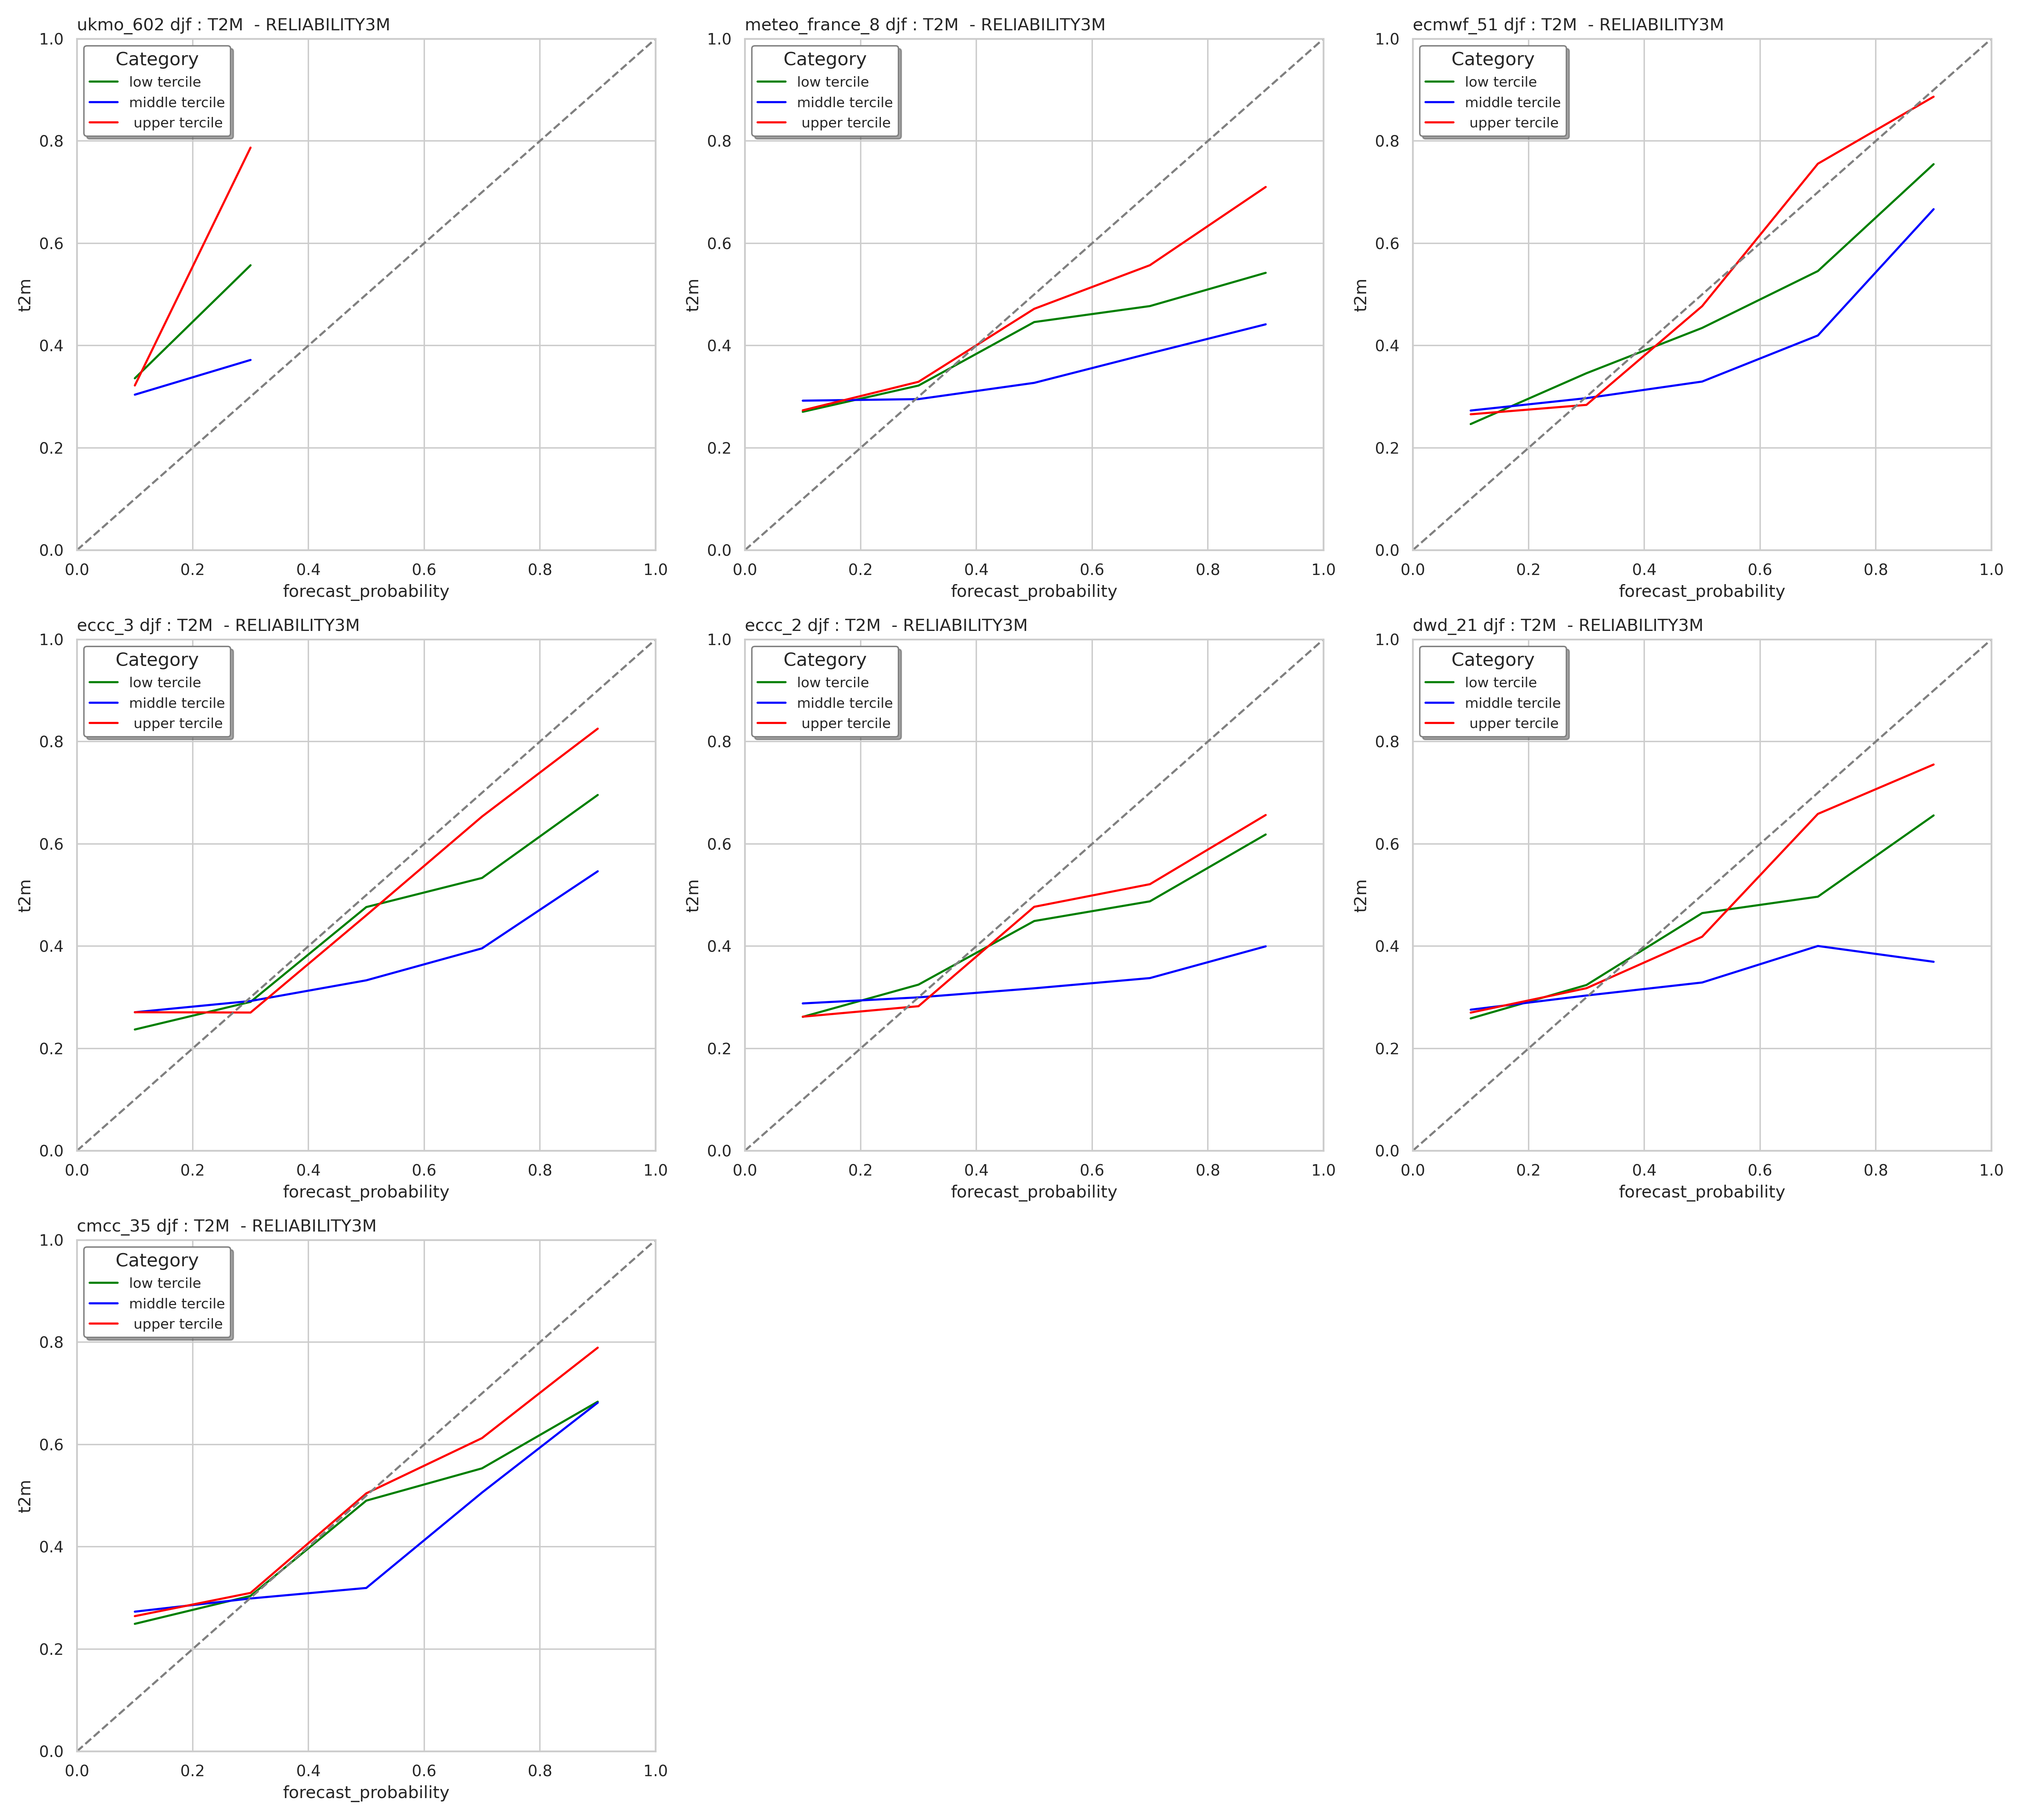
\includegraphics[width=1\linewidth]{plots/prob/rela/rela_diagram_t2m_djf.png}
    \caption{temperature reliabilty maps for djf}
    \label{CORR_mam_t2m.png}
\end{figure}

For the DJF season, the reliability diagrams show that most models exhibit similar performance, with the exception of UKMO, which significantly overestimates probabilities across all categories. For ECMWF, there is a noticeable overestimation in the upper tercile (warm extremes) starting at a forecast probability of approximately 0.6, indicating that the model tends to assign higher probabilities to warm events compared to their observed frequencies. Conversely, ECMWF shows a systematic underestimation for both the lower and middle terciles across most probabilities. For the remaining models, except UKMO, there is a general trend of underestimation across all three categories, beginning at forecast probabilities around 0.5. This pattern suggests that while the models capture some aspects of the observed temperature distribution, they struggle to provide accurate probabilities for more extreme or moderate conditions, especially at higher forecast probabilities. These results highlight the challenges faced by the models in reliably predicting temperature outcomes during the winter season (DJF), particularly for extreme categories.
For the other three seasons (JJA, MAM, and SON), the reliability diagrams reveal a general tendency for most models to underestimate probabilities across all tercile categories, starting at approximately 0.4. This underestimation indicates that the models tend to be over-cautious, predicting lower probabilities than what is observed in reality. However, UKMO still stands out as an exception, showing a consistent overestimation across the forecast range, particularly for higher probabilities. This suggests that UKMO tends to assign excessively high probabilities to events that occur less frequently than predicted, which reduces its reliability. Overall, this recurring underestimation in the majority of models highlights their difficulty in accurately capturing the likelihood of temperature outcomes, especially beyond moderate probabilities. 

\begin{figure}[H]
    \centering
    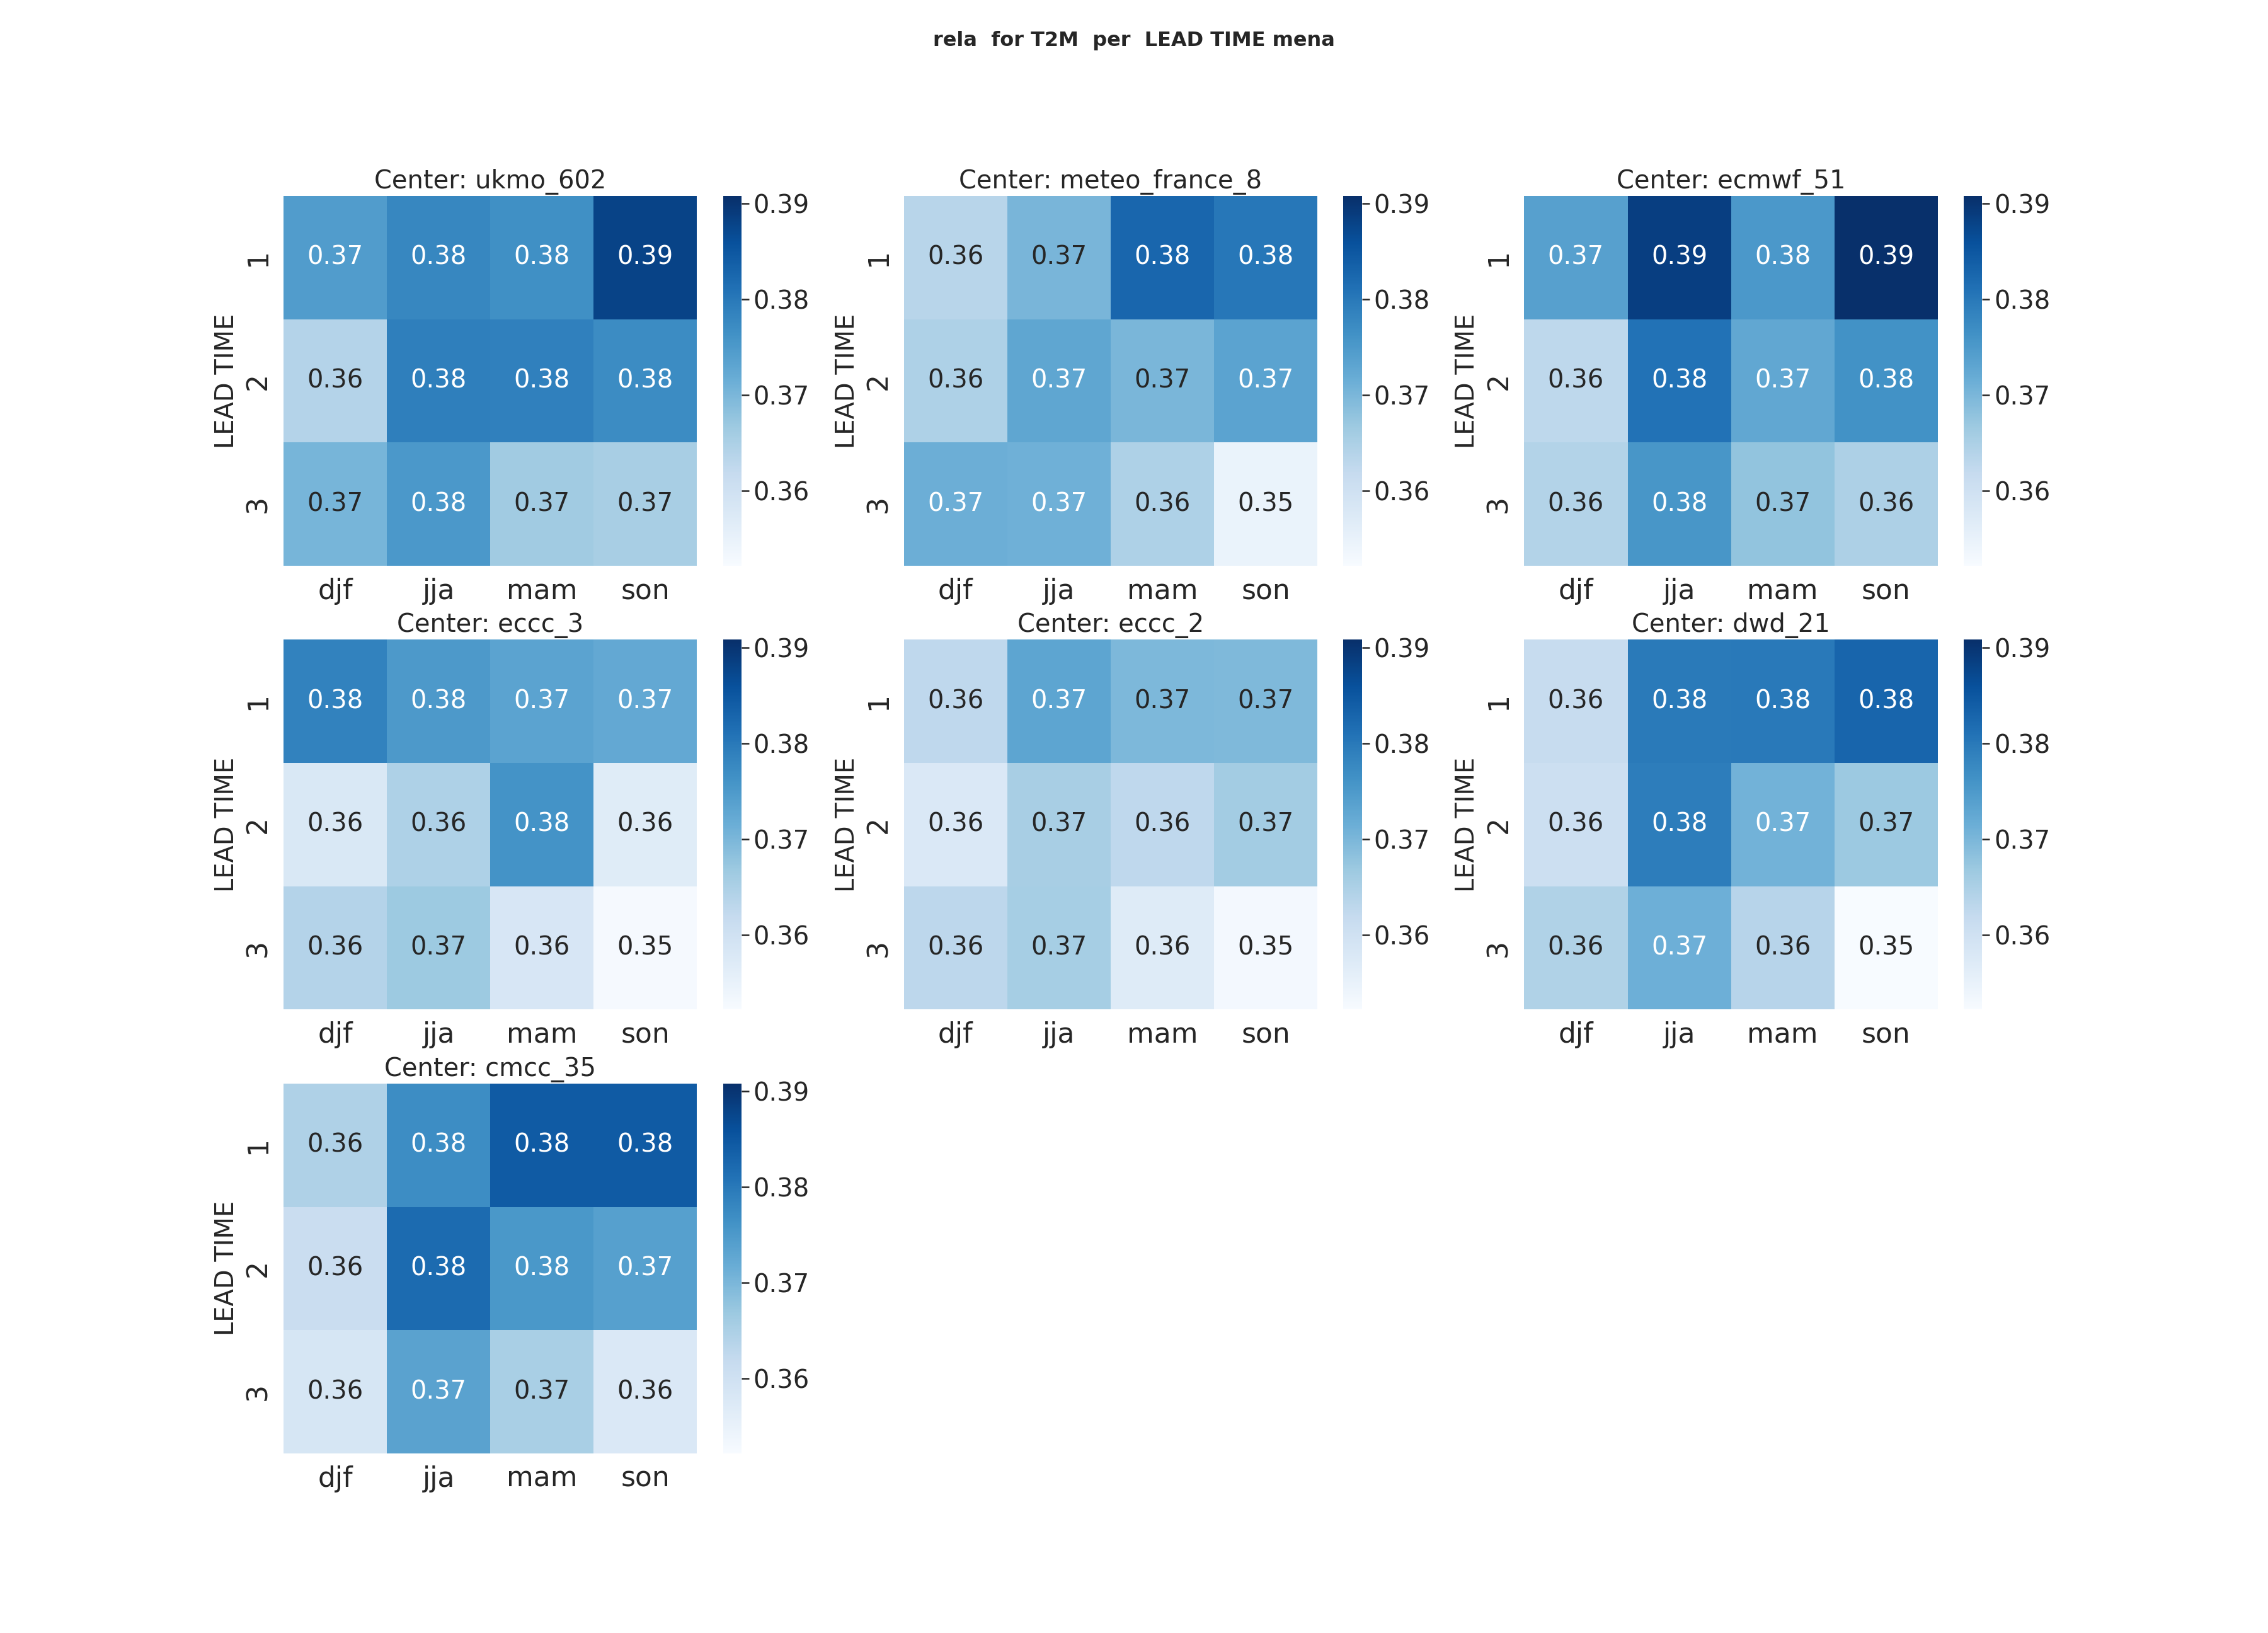
\includegraphics[width=1\linewidth]{plots/prob/rela/rela_T2M_mena.png}
    \caption{temperature reliabilty heatmap}
    \label{CORR_mam_t2m.png}
\end{figure}
The heatmap further confirms the analyses derived from the reliability diagrams. It highlights similar trends observed across the models and seasons.Conversely, UKMO continues to stand out with its consistent overestimation of probabilities, aligning with the overconfidence seen in the reliability diagrams. This agreement between the heatmap and the reliability curves strengthens confidence in the identified patterns .




\subsubsection{The ranked probability score }

The Ranked Probability Score (RPS) provides a valuable measure of forecast performance by evaluating the accuracy of probabilistic predictions across different categories. It combines both the skill in predicting the occurrence of events and the sharpness of the forecast distribution. By comparing the forecasted probability distribution against the observed outcomes, the RPS quantifies the deviation between the predicted and actual probabilities. A lower RPS value indicates better forecast accuracy, reflecting both how well the forecast aligns with observed frequencies and how well it discriminates between different probability categories. This metric helps to identify which models offer the most reliable probabilistic predictions, particularly in terms of capturing the likelihood of various temperature outcomes within a given forecast period.
\begin{figure}[H]
    \centering
    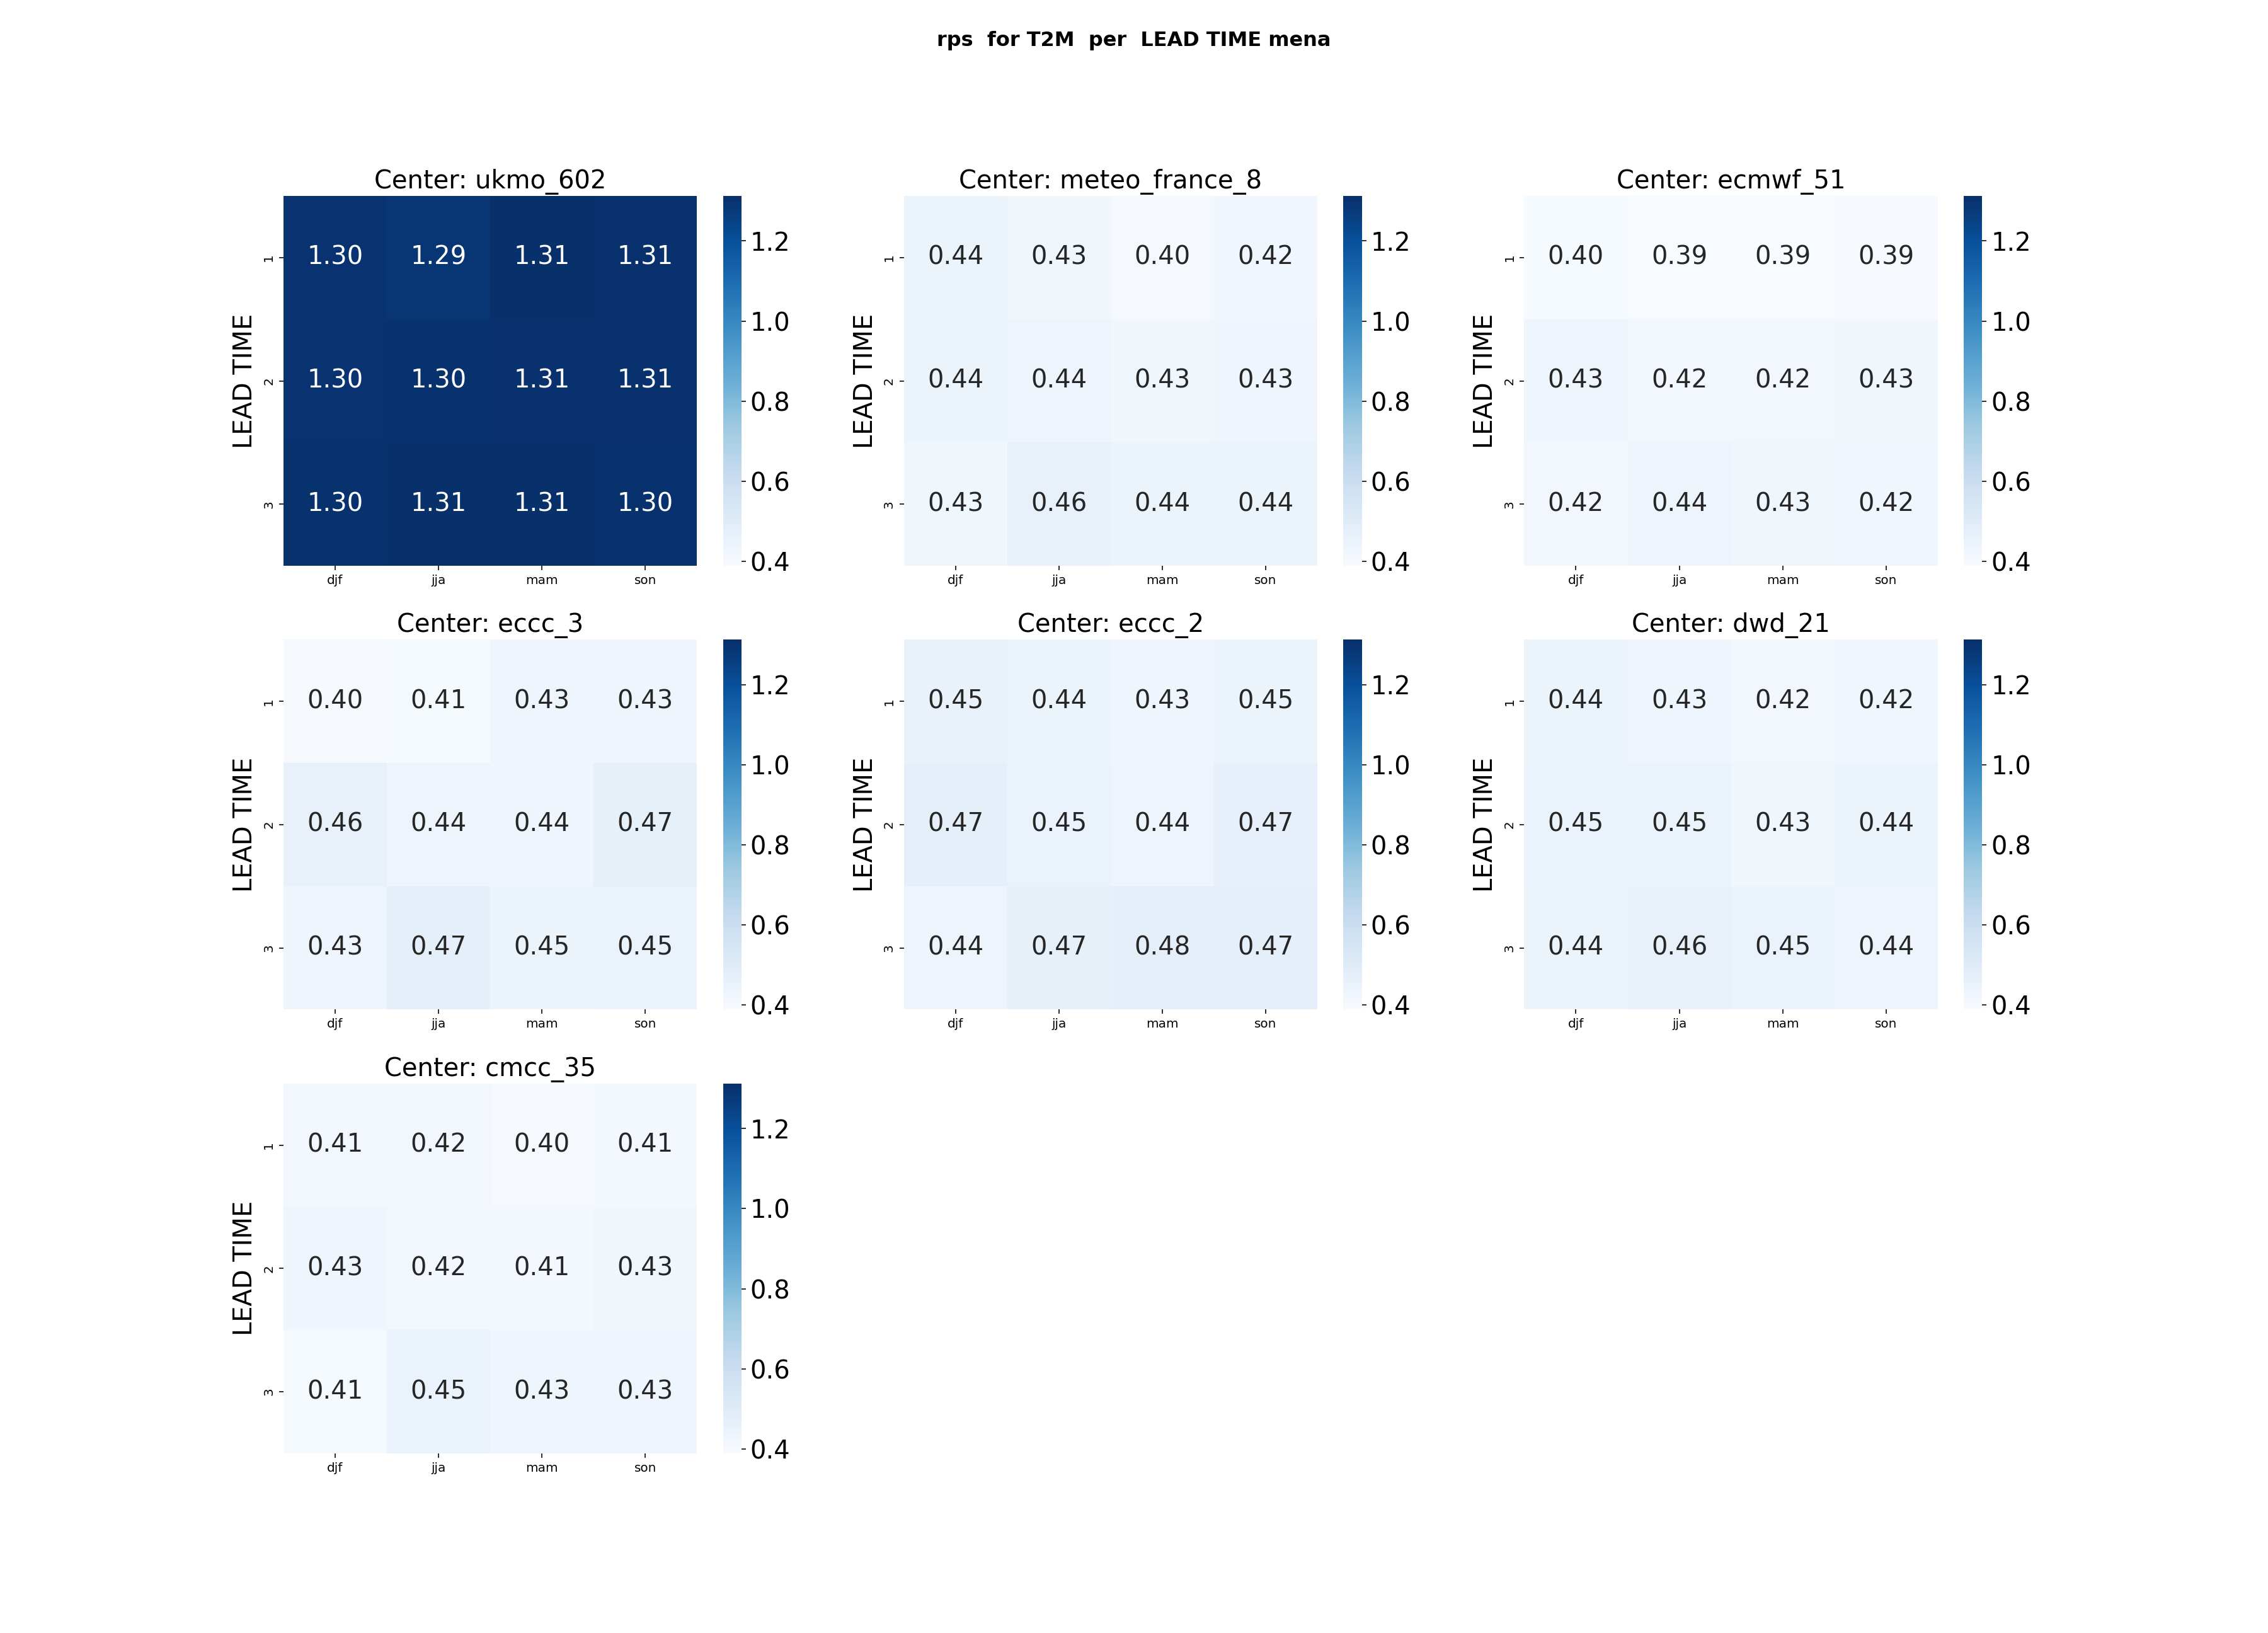
\includegraphics[width=1\linewidth]{plots/prob/rps/rps_T2M_mena.png}
    \caption{Temperature RPS  heatmaps for all the seasons per categories}
    \label{fig:CORR_djf_t2m}
\end{figure}
The figure displaying the Ranked Probability Score (RPS) for different climate models and seasonal periods provides a detailed view of model performance across various start months (DJF, JJA, MAM, SON). Each cell in the matrix represents the RPS value for a specific model and season combination, with the color intensity indicating how well the forecast probabilities match the observed data.

From this figure, it is evident that ECMWF consistently shows lower RPS values, indicating better predictive accuracy across different seasons. This suggests that ECMWF's forecasts are more closely aligned with observed temperature variability. The relatively higher RPS values for  UKMO model underscore their challenges in accurately capturing temperature variations. 

\subsubsection{Receiver Operating Characteristic}
The ROC (Receiver Operating Characteristic) curve is an important tool for evaluating the performance of predictive models, particularly in the context of probabilistic forecasts. It provides a graphical representation of the trade-off between the true positive rate  and the false positive rate  across various threshold levels.

\begin{figure}[H]
    \centering
    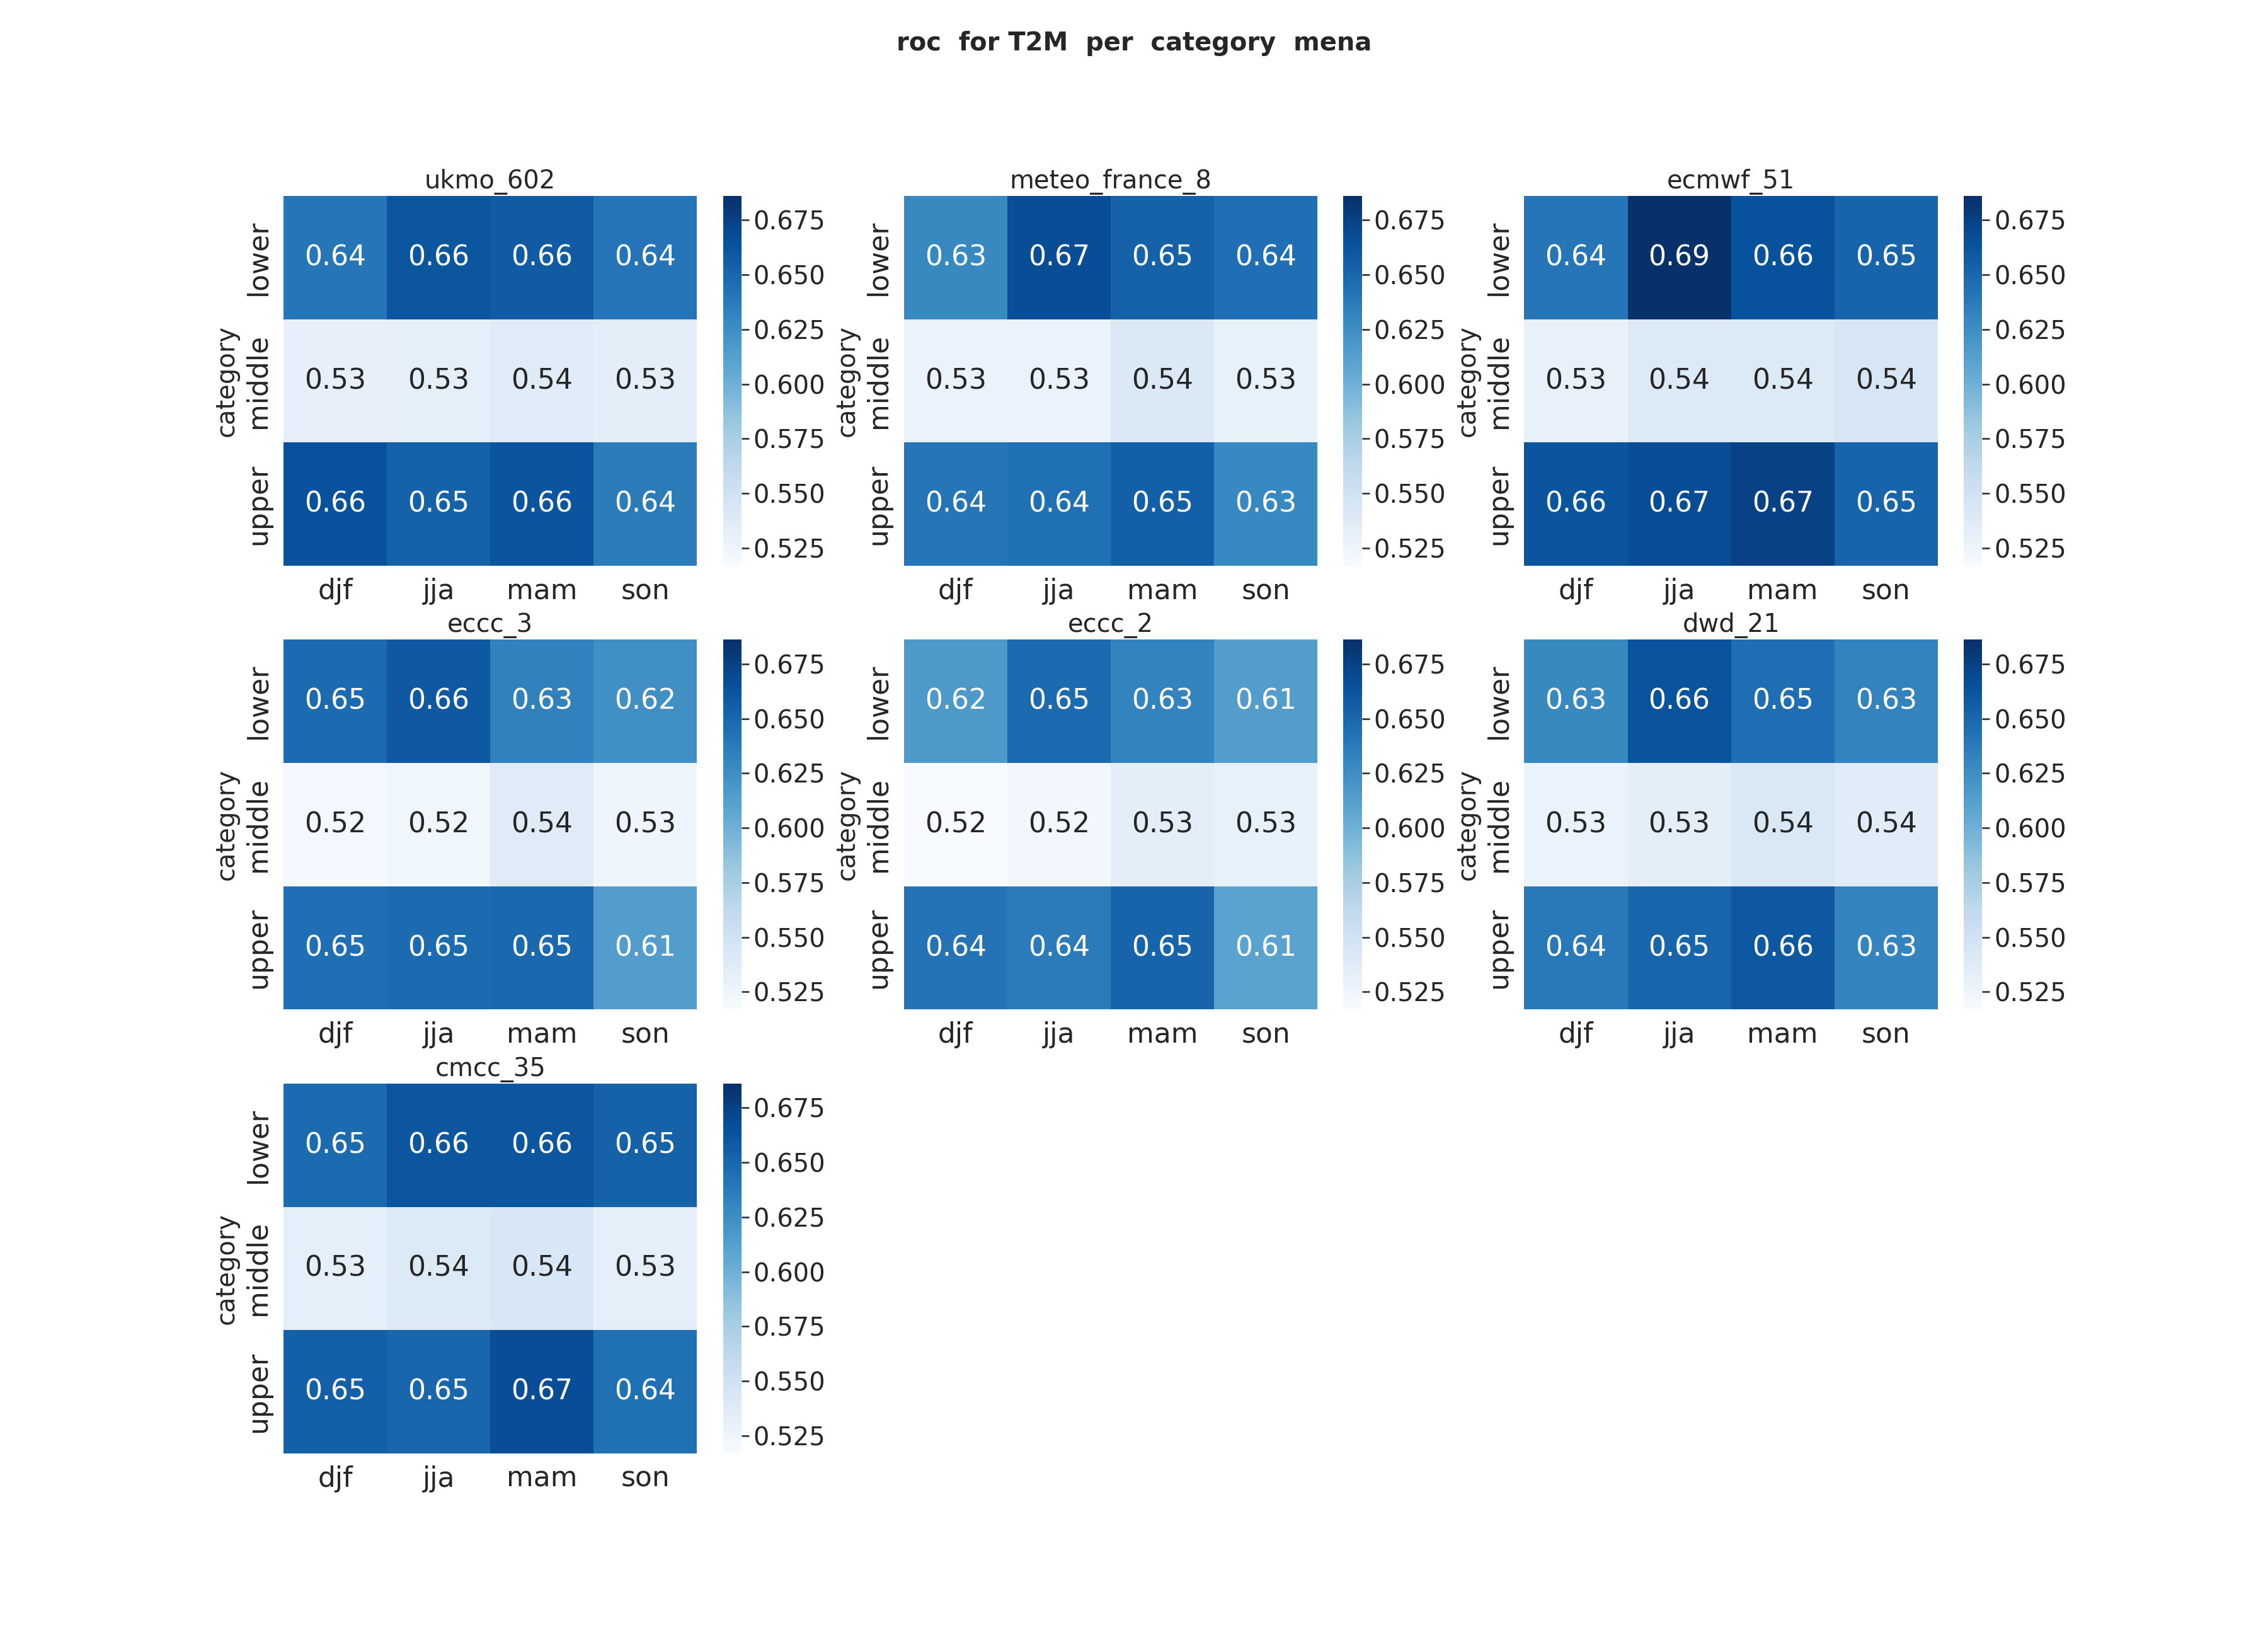
\includegraphics[width=1\linewidth]{plots/prob/roc/roc_T2M_category_mena.png}
    \caption{Temperature AUC  heatmaps }
    \label{fig:CORR_djf_t2m}
\end{figure}


Models generally exhibit similar performance, as indicated by the high Area Under the ROC Curve (AUC) values, which reflect their ability to effectively discriminate between predicted probabilities and observed outcomes. Unlike the reliability metric, where UKMO showed weaker performance, it performs relatively well in terms of the AUC, demonstrating good skill in distinguishing between forecasted events and non-events. Similar to the findings with the Brier Score (BS), the "middle" probability category tends to show weaker performance compared to the "lower" and "upper" categories. This highlights the models' greater sensitivity in accurately predicting events with extreme probabilities (high or low), but reduced skill for moderate probability scenarios. This consistency across metrics underscores the need to address forecast performance specifically in the middle category to further improve model predictions.


\subsubsection{Relative operating characteristics Skill Score}
ROCSS provides an assessment of a model's ability to discriminate between observed and forecasted events relative to a reference model, often a climatological or random forecast. A higher ROCSS indicates that the model has skill in distinguishing between occurrences and non-occurrences of an event, while a score close to zero suggests no significant improvement over the reference

\begin{figure}[H]
    \centering
    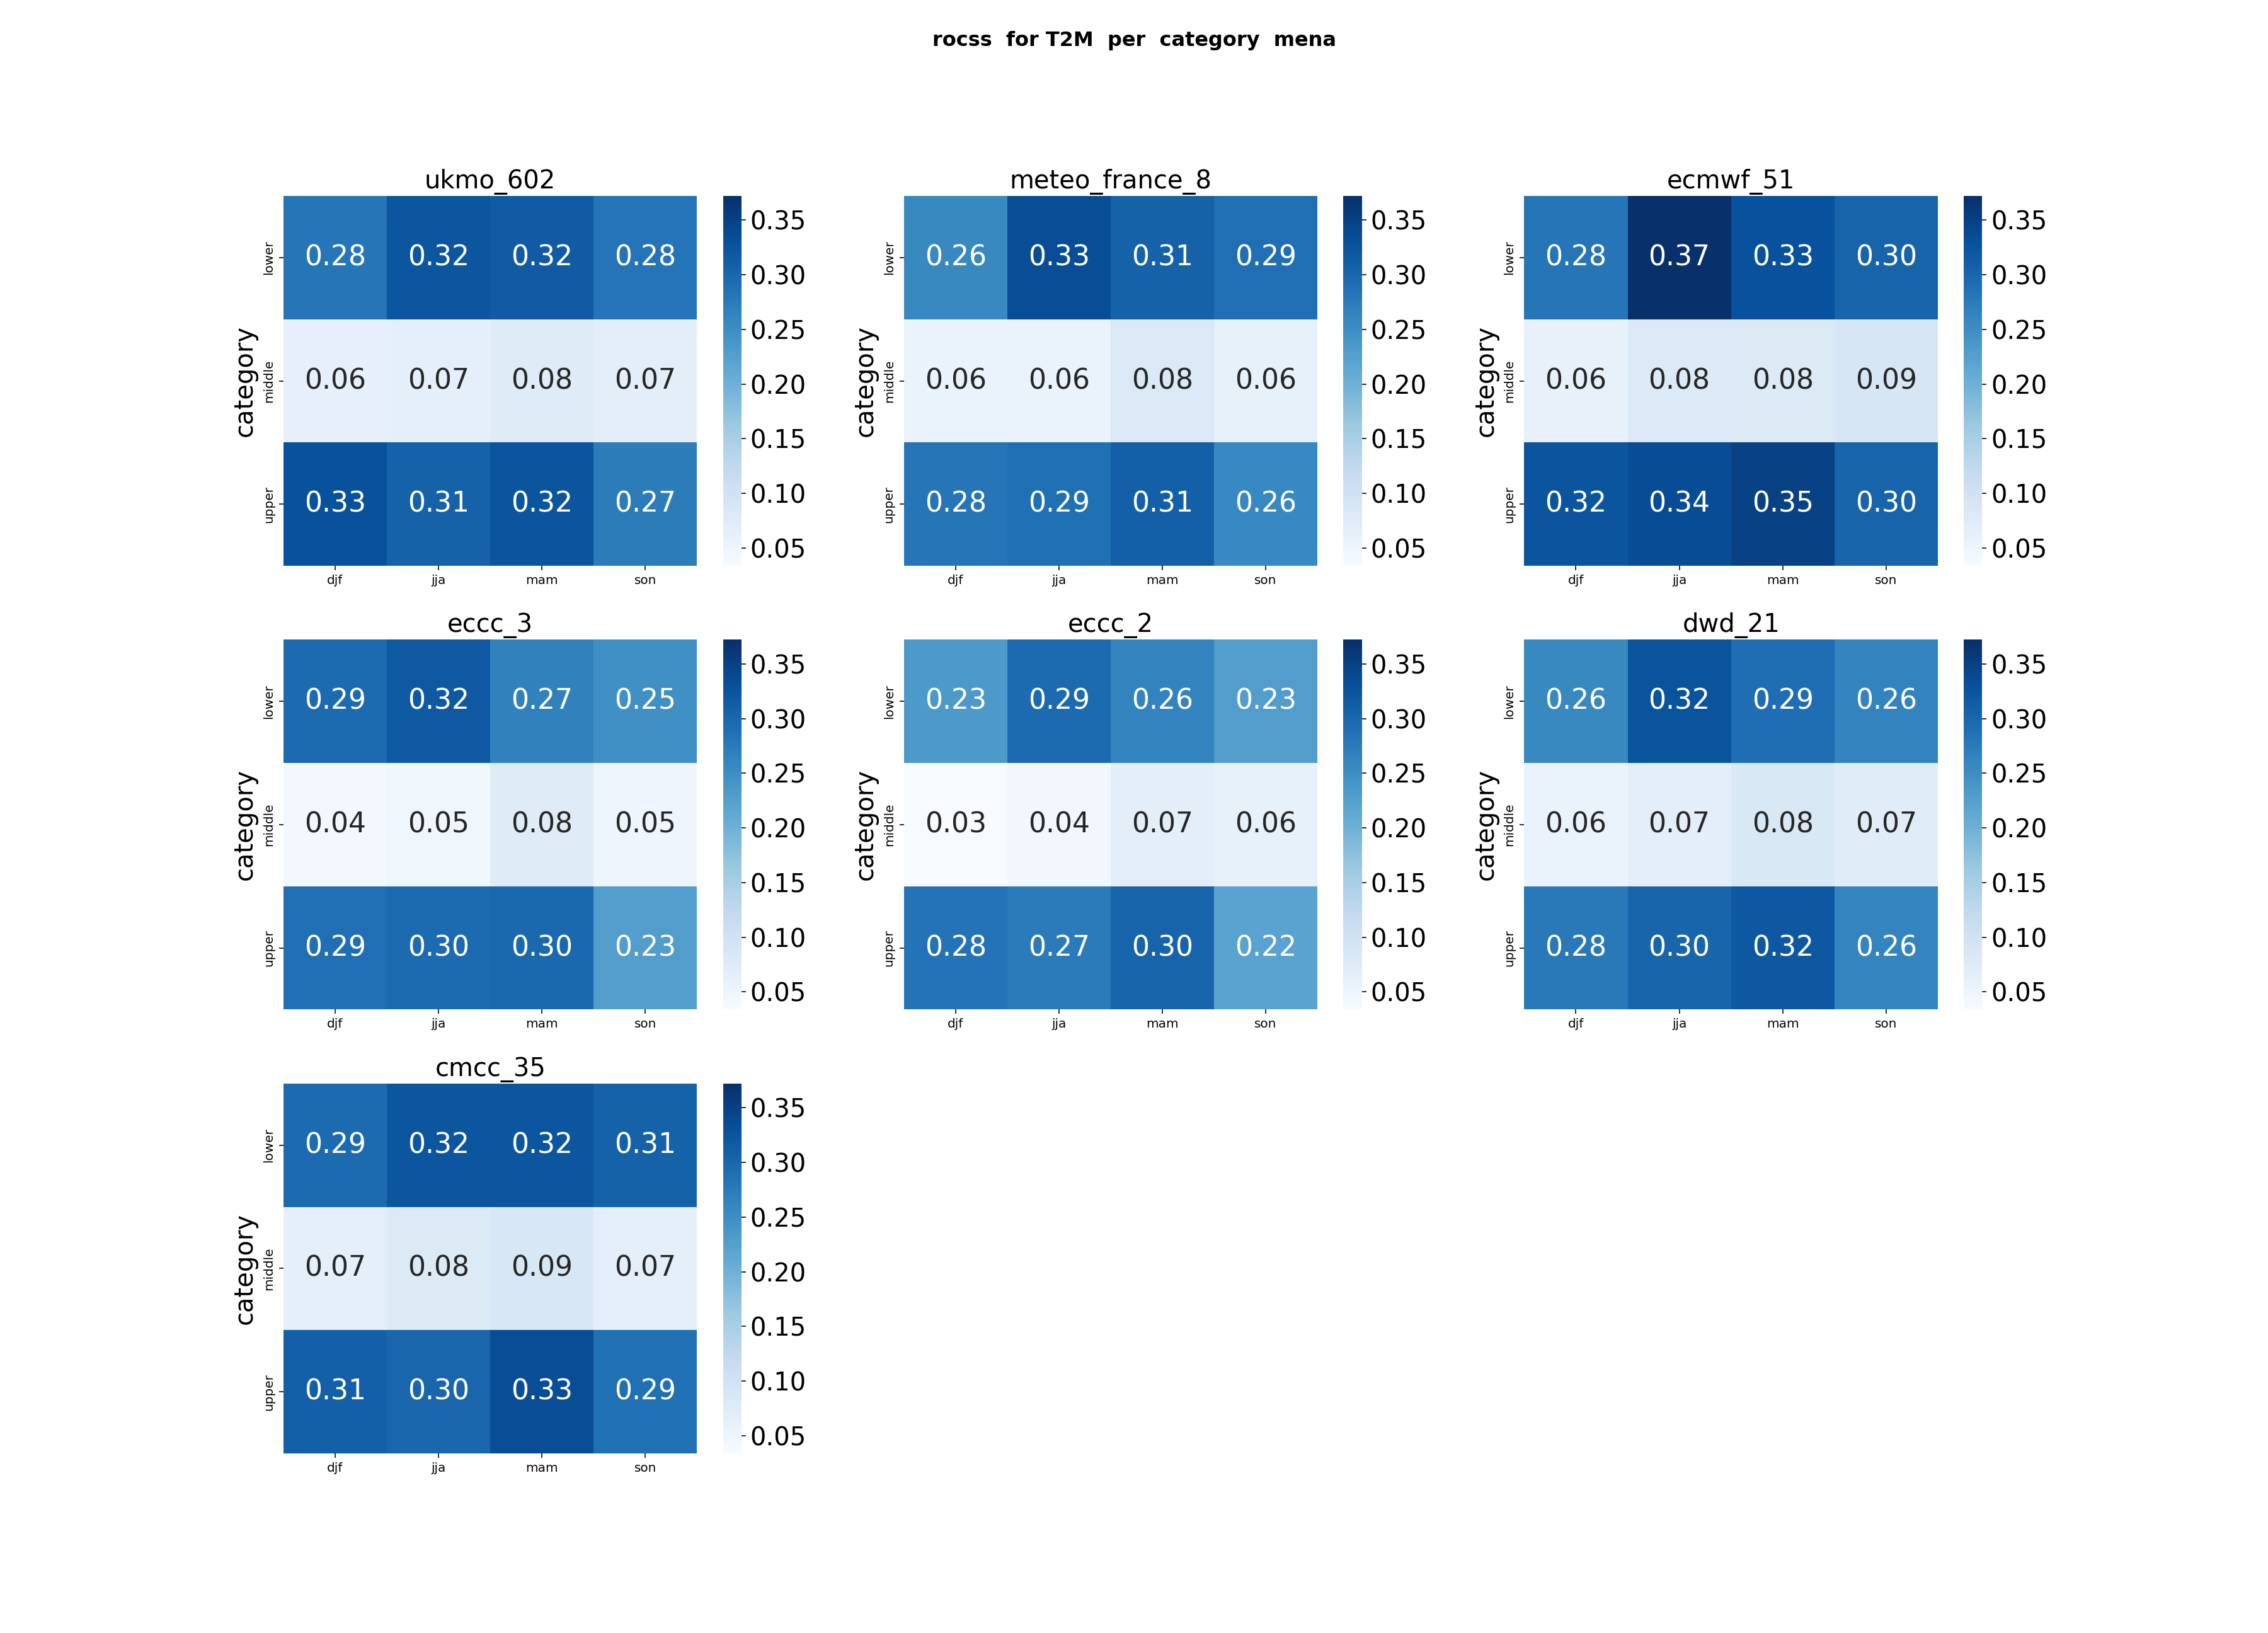
\includegraphics[width=1\linewidth]{plots/prob/rocss/rocss_T2M_category_mena.png}
    \caption{Temperature ROCSS  heatmaps for MENA region }
    \label{fig:CORR_djf_t2m}
\end{figure}. 
The models generally demonstrate consistent and positive skill, highlighting their ability to discriminate between observed and forecasted events. UKMO, which showed weaker performance in reliability metrics, continues to perform well in terms of ROCSS, confirming its relative robustness in event discrimination. Additionally, as observed with the ROC scores, the "middle" category exhibits lower performance compared to the "lower" and "upper" categories. This indicates that while the models excel at predicting extreme events with high or low probabilities, their ability to capture moderate probability events remains limited.








\section{PRECIPITATIONS}
IN general, the forecast of precipitations is more complicated than temperature, thus the scores are a little less good for this part especially the deterministic ones. 
\subsection{Deterministic Evaluation Metrics}

\subsubsection{ACC}

\begin{figure}[H]
	\centering
	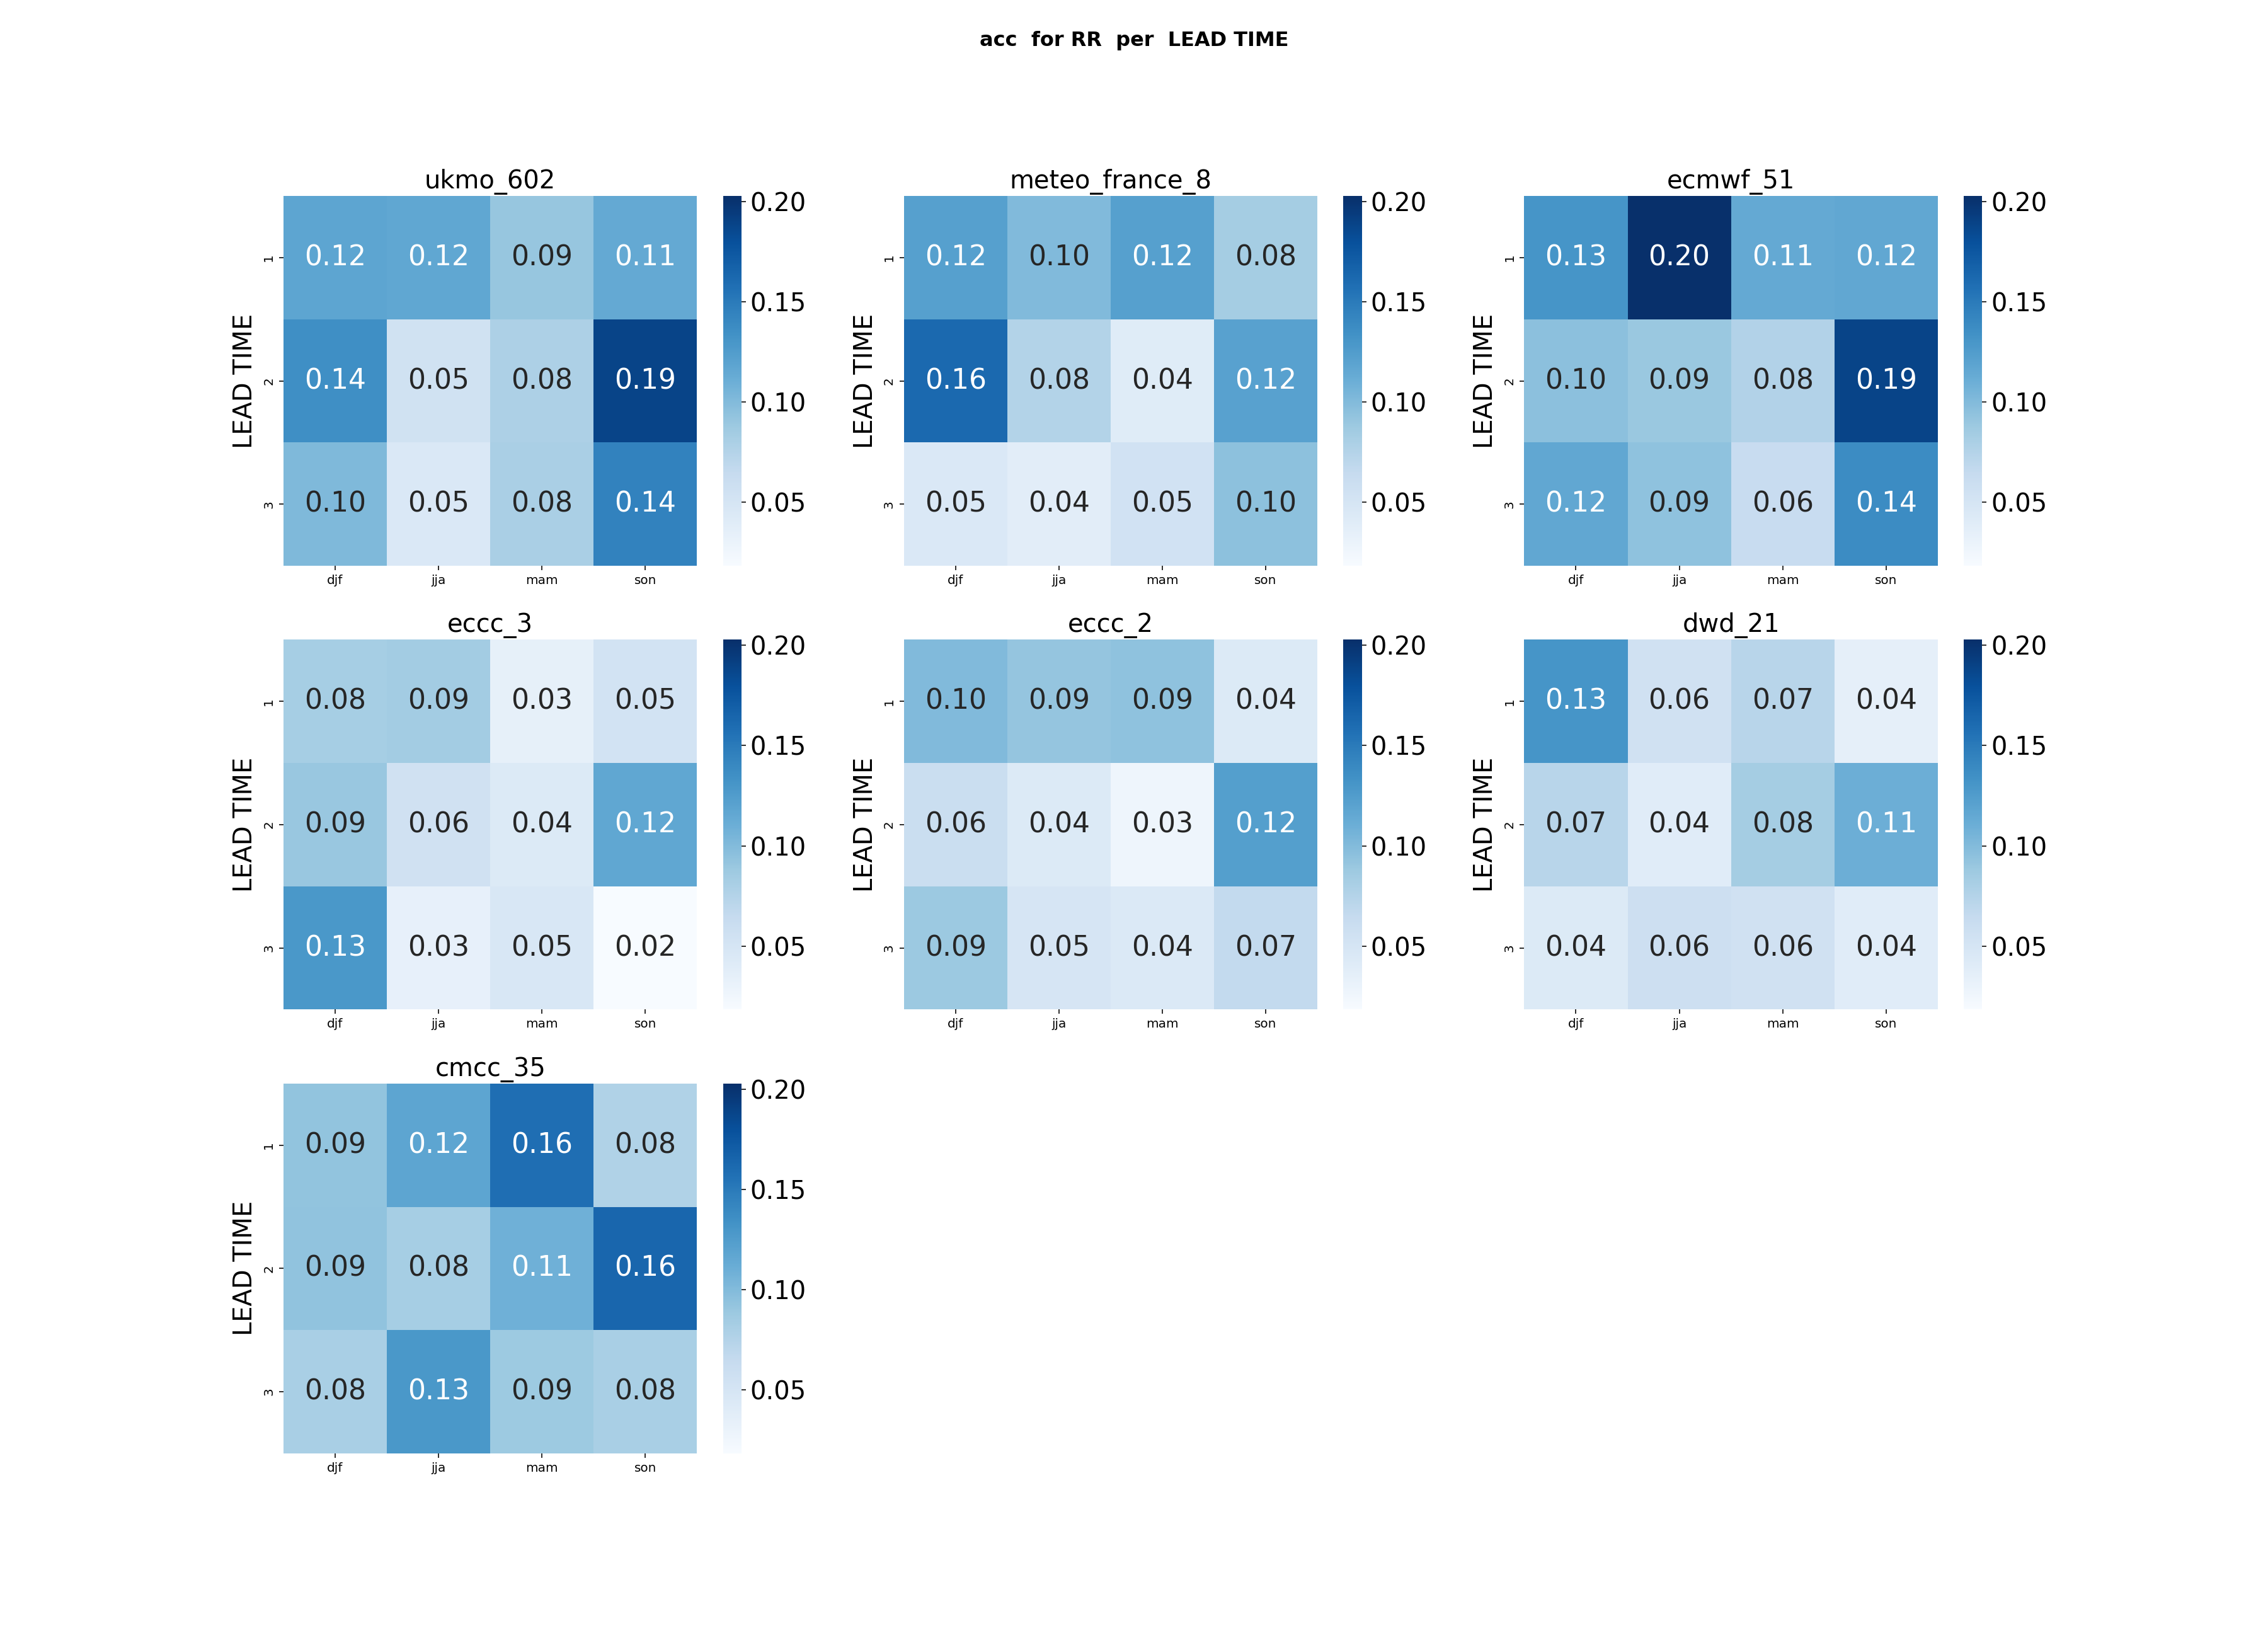
\includegraphics[scale=0.25]{plots/det/acc/acc_RR_mena.png}
	\caption{The Heatmap of acc for the mena region for every period \textbf{\textit{(1 for perfect Correlation)} }}
\end{figure}
The acc is moderate for all centers; however, the best models are \textbf{\textit{ECMWF, UKMO, and CMCC-35}}. There is no clear variability in performance along lead-time. For SON, the performance is good at lead-time 2 for all centers. As for the other seasons, the performance is generally strong at the 1st lead-time but decreases with increasing lead-time.
Hence, Meteo-France also shows good performance, but it decreases significantly over time.



\begin{figure}[H]
\centering
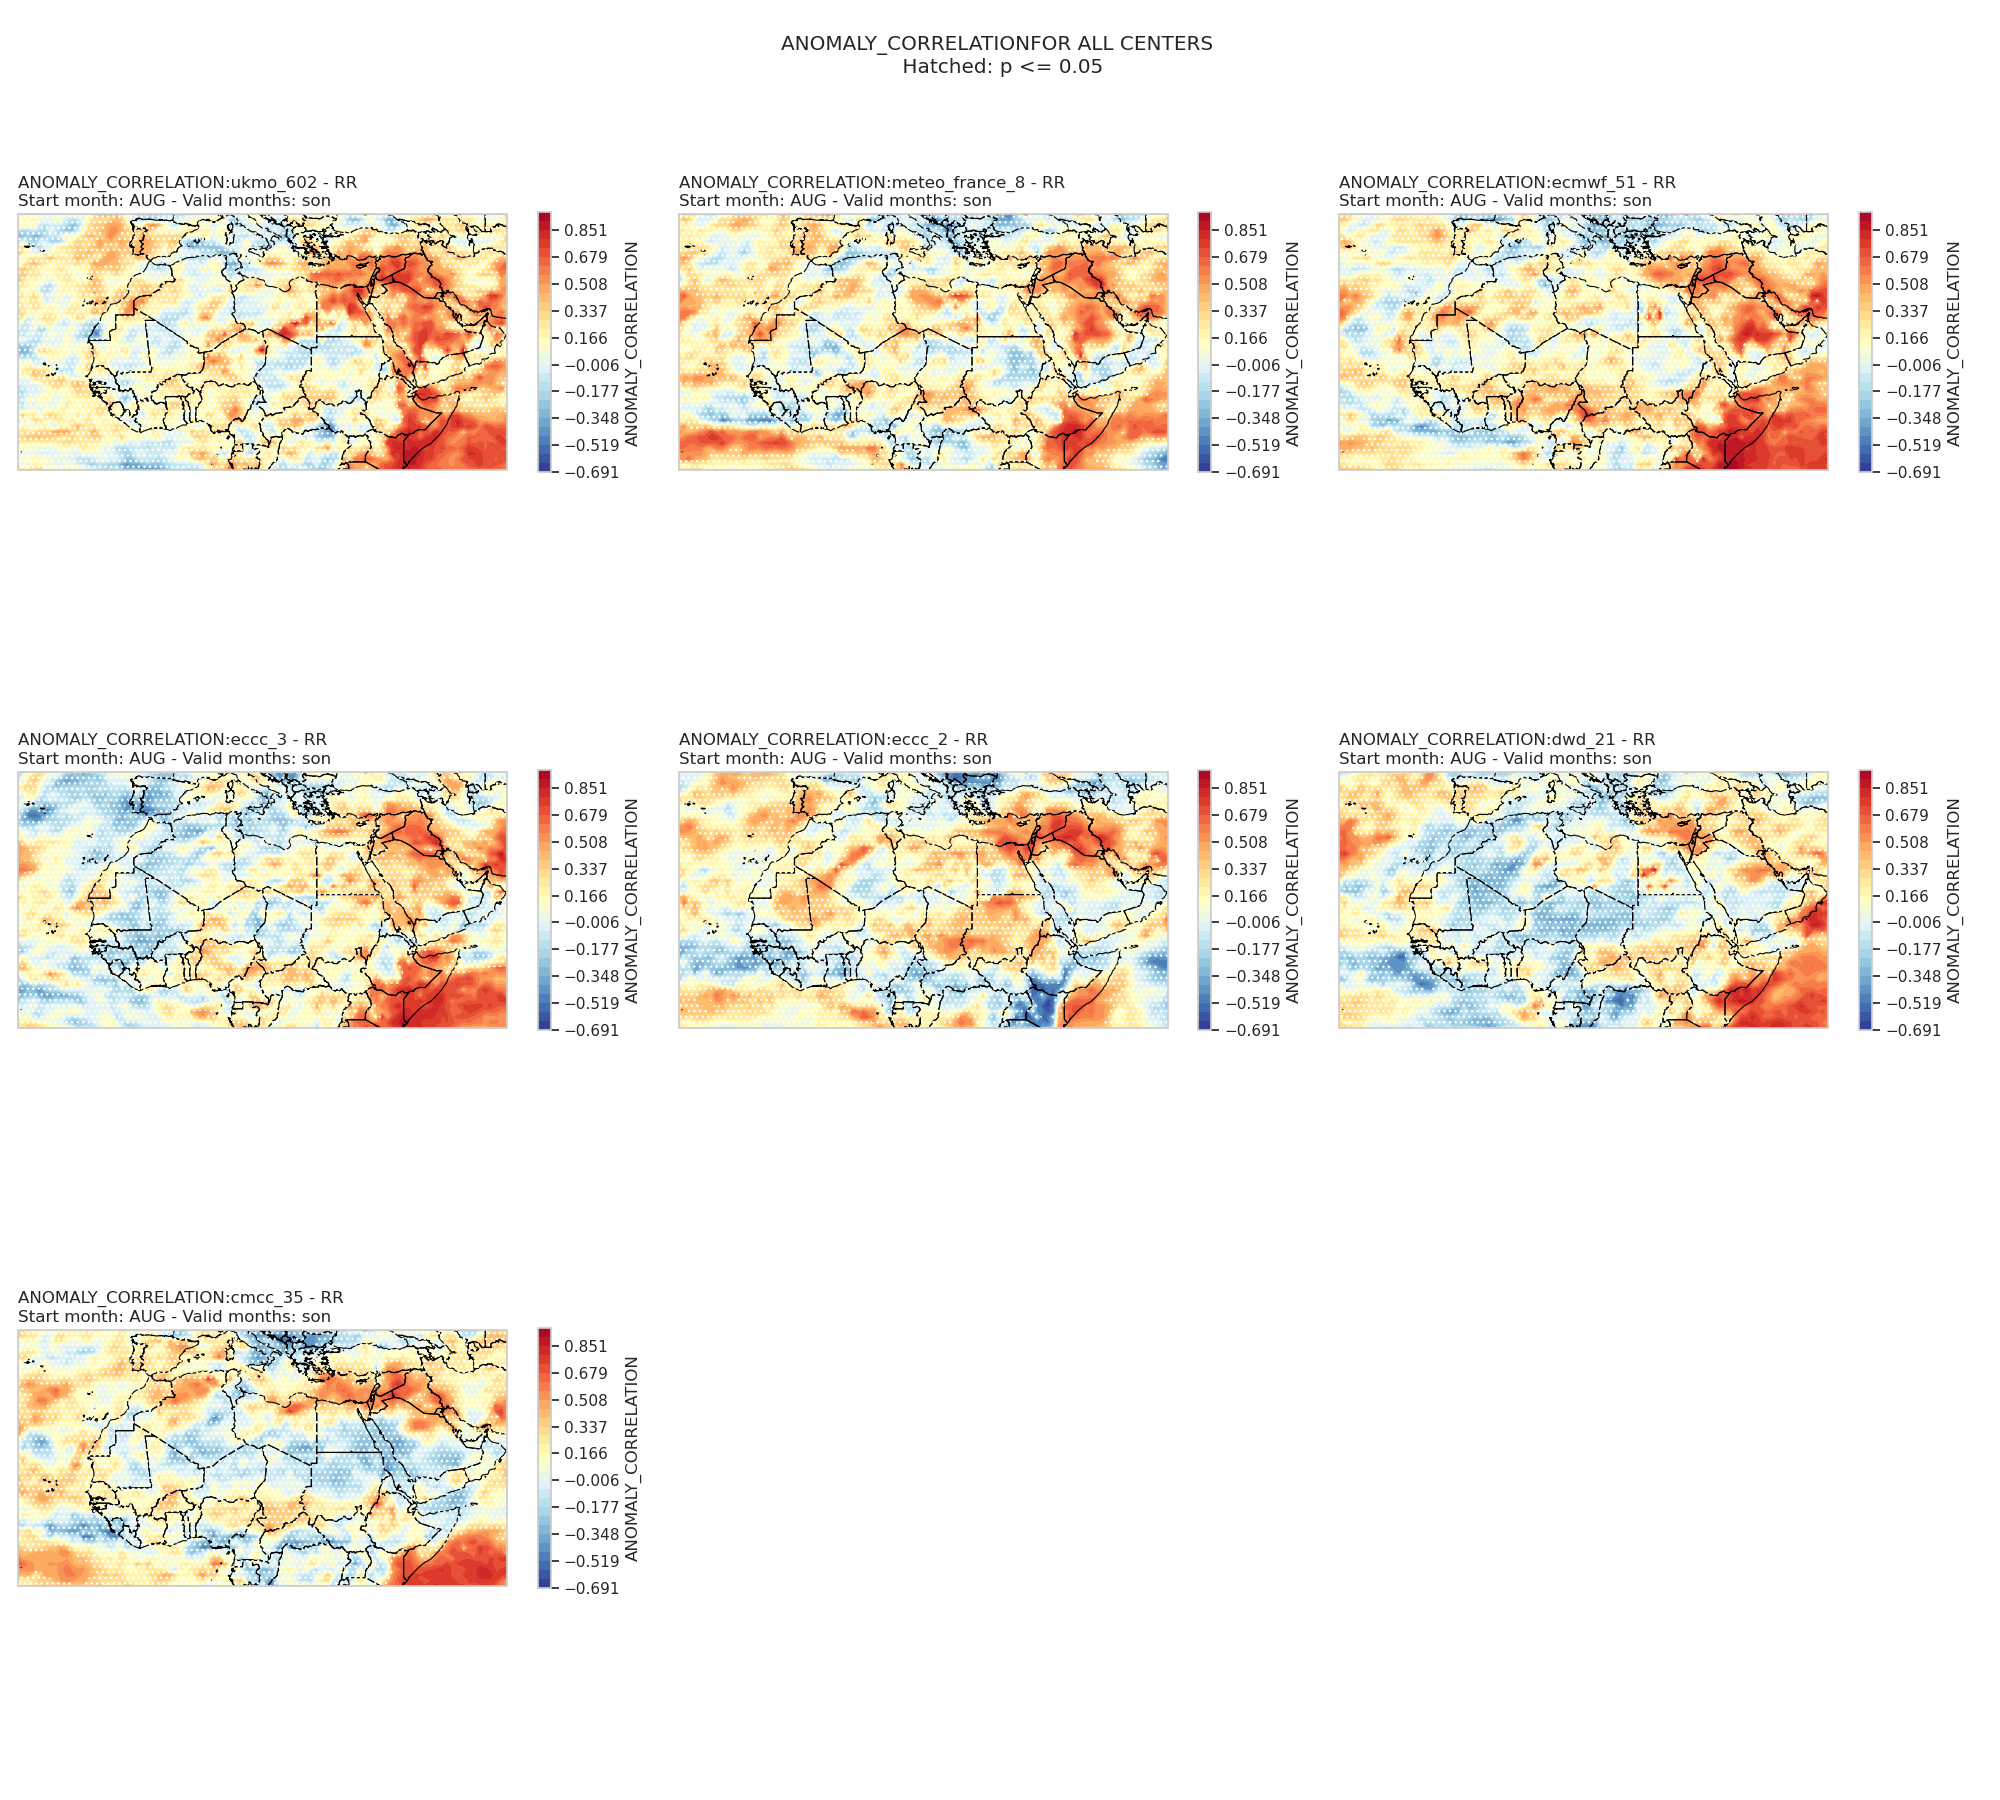
\includegraphics[scale=0.3]{plots/det/acc/ANOMALY_CORRELATION_son_RR.png}
\caption{3-months Rolling mean of Anomaly Correlation in MENA Region for all centers SON}
\end{figure}
For temperature, the models demonstrate the best performance in the tropical regions. However, for precipitation, the situation is different. Hence the results show good performance during SON, where the Arabian Peninsula and  East Africa exhibit the highest performance.
\begin{figure}[H]
\centering
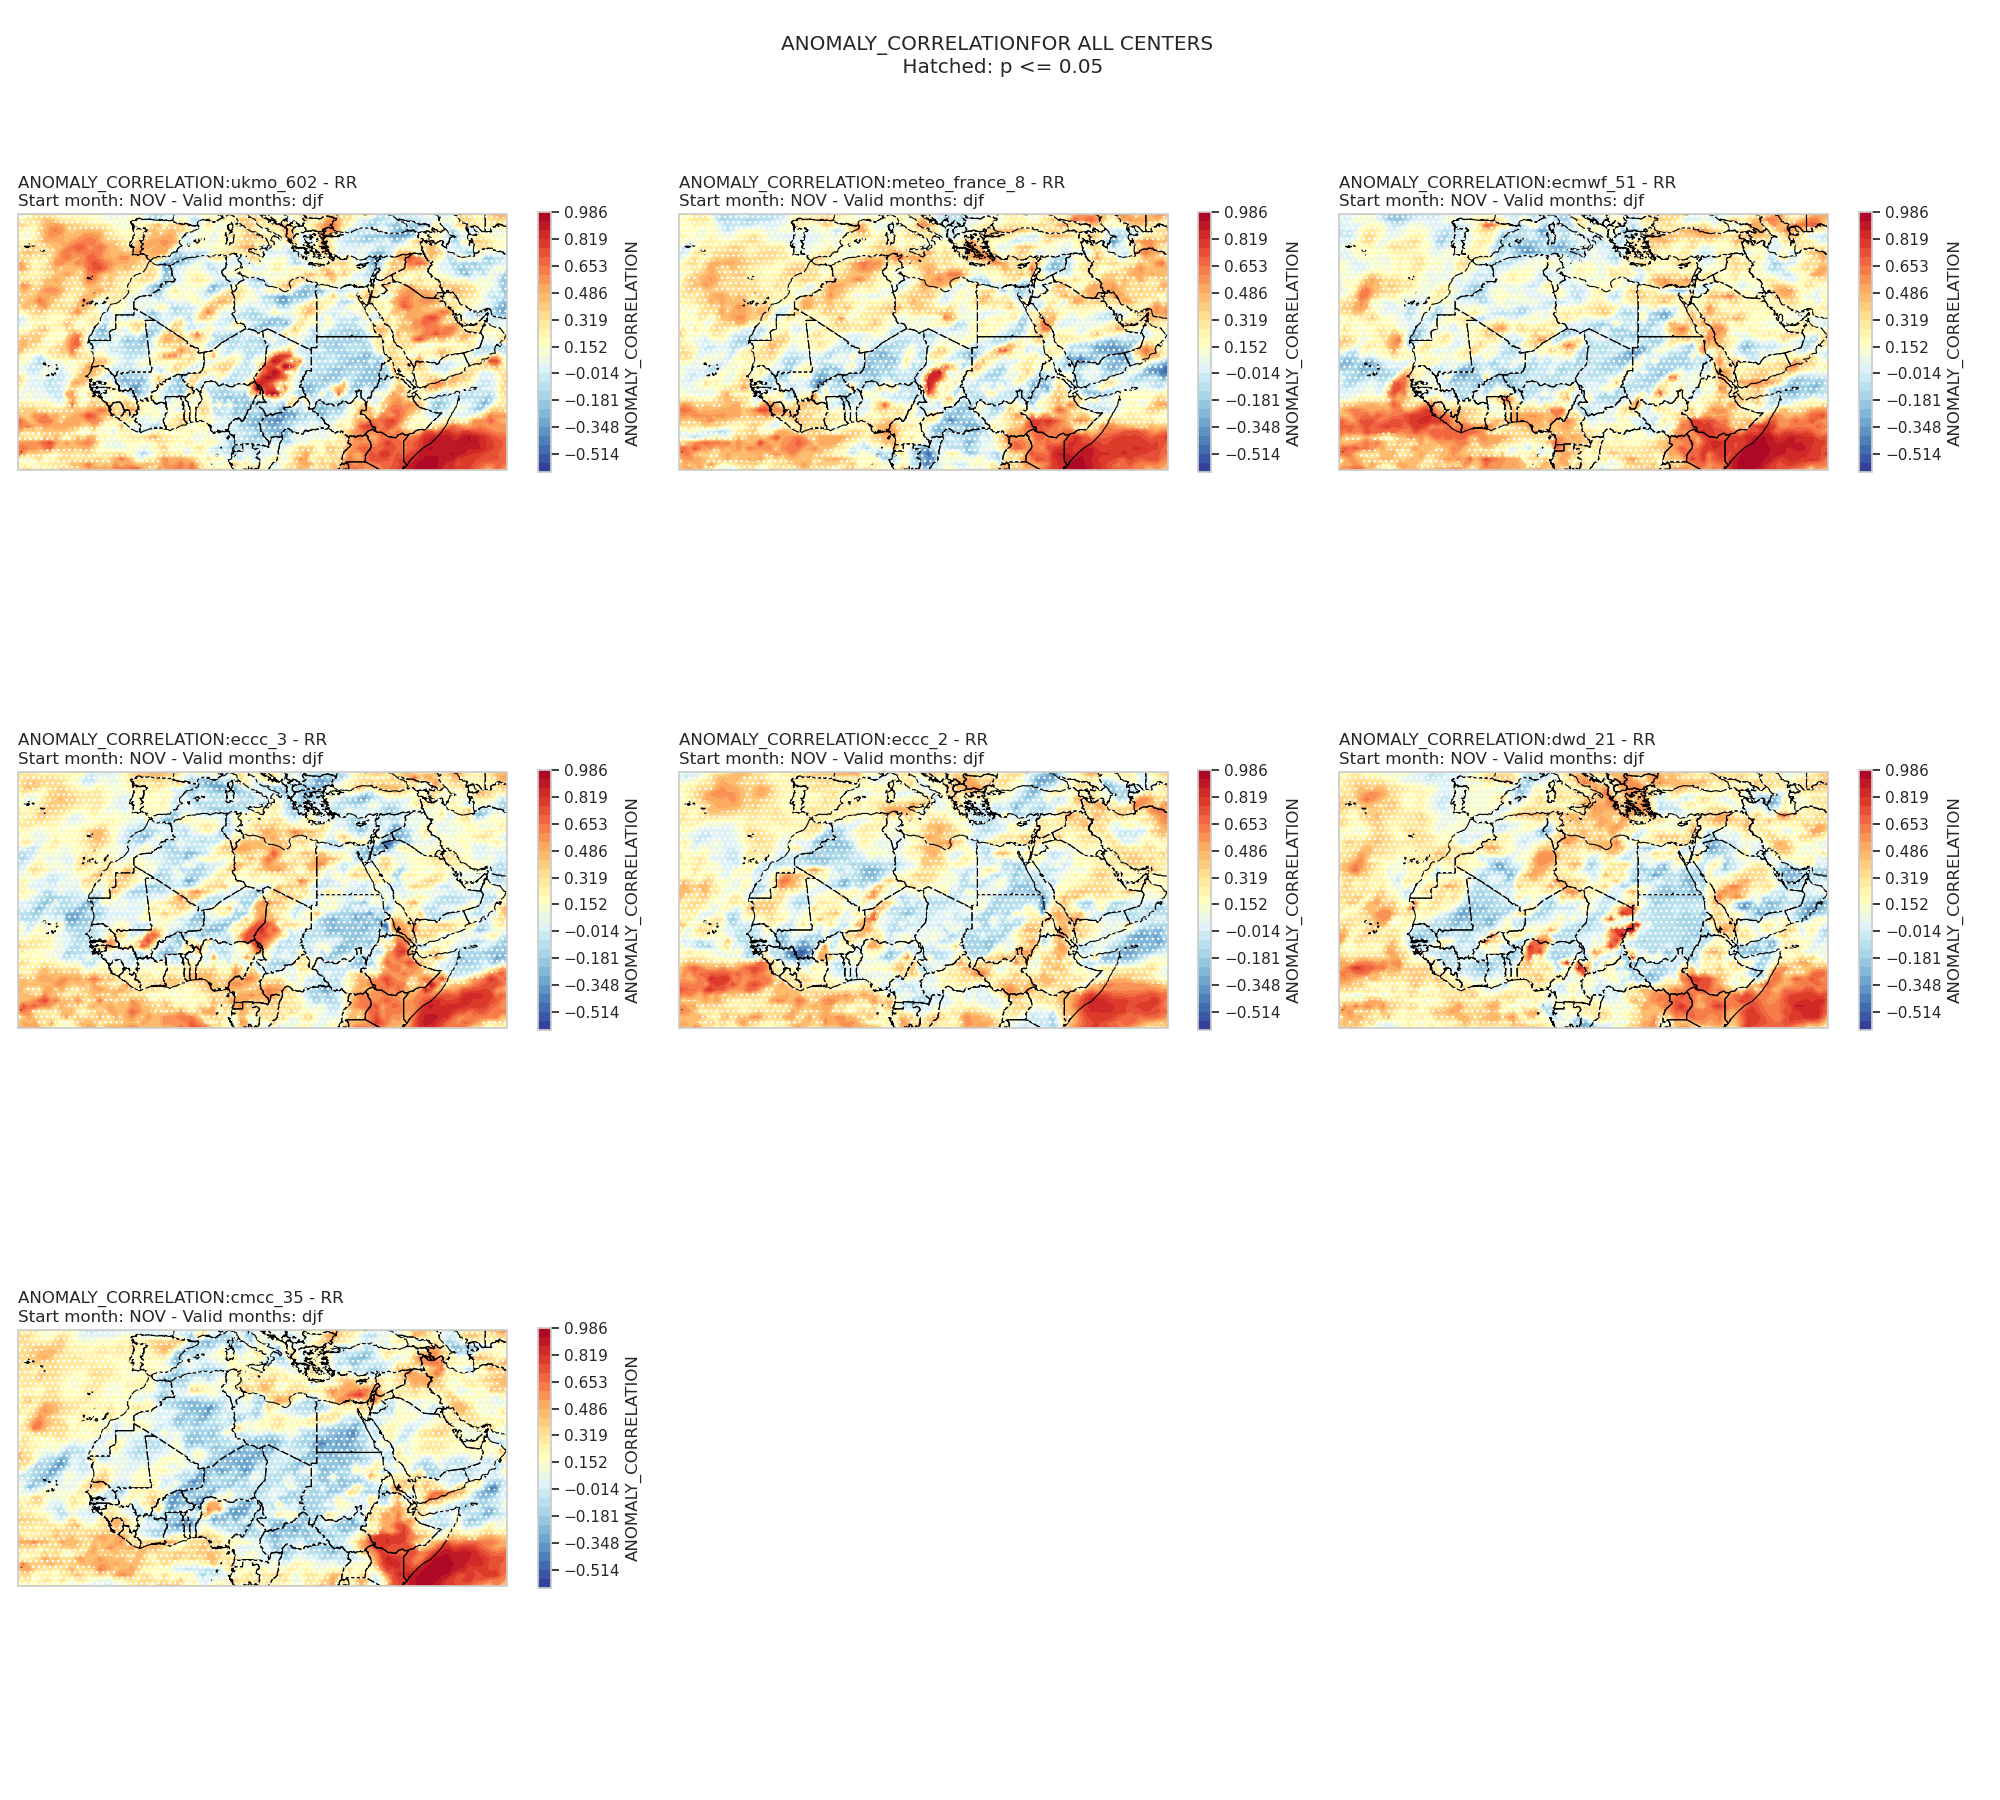
\includegraphics[scale=0.3]{plots/det/acc/ANOMALY_CORRELATION_djf_RR.png}
\caption{3-months Rolling mean of Anomaly Correlation in MENA Region for all centers DJF}
\end{figure}

The 3-month rolling mean for DJF acc shows that the best models are \textbf{\textit{ECMWF, UKMO, and Meteo-France}}. The acc is significant across most of the MENA region, except in the east of Africa. Thus, for all centers the East of Africa have the highest score. However, the \textbf{\textit{ecmwf and ukmo}} show good performance for 


 
For SON, the situation is generally better than for DJF in the Arabian peninsula. In general, \textbf{\textit{ECMWF and Meteo-France}} are the best. Nevertheless, the correlation isn't significant in the east of africa and the north of the Arabian peninsula despite of the high acc.


\subsubsection{RMSE}
 
for the Root Mean Squared Error, the best models shown in the heatmap below are \textbf{\textit{DWD, ECMWF and UKMO}}. The RMSE score demonstrate a moderate performance for all models especially \textbf{\textit{DWD, ECMWF and UKMO}}. The performance is stable over lead-times and it is much better for djf in all centers.

\begin{figure}[H]
\centering
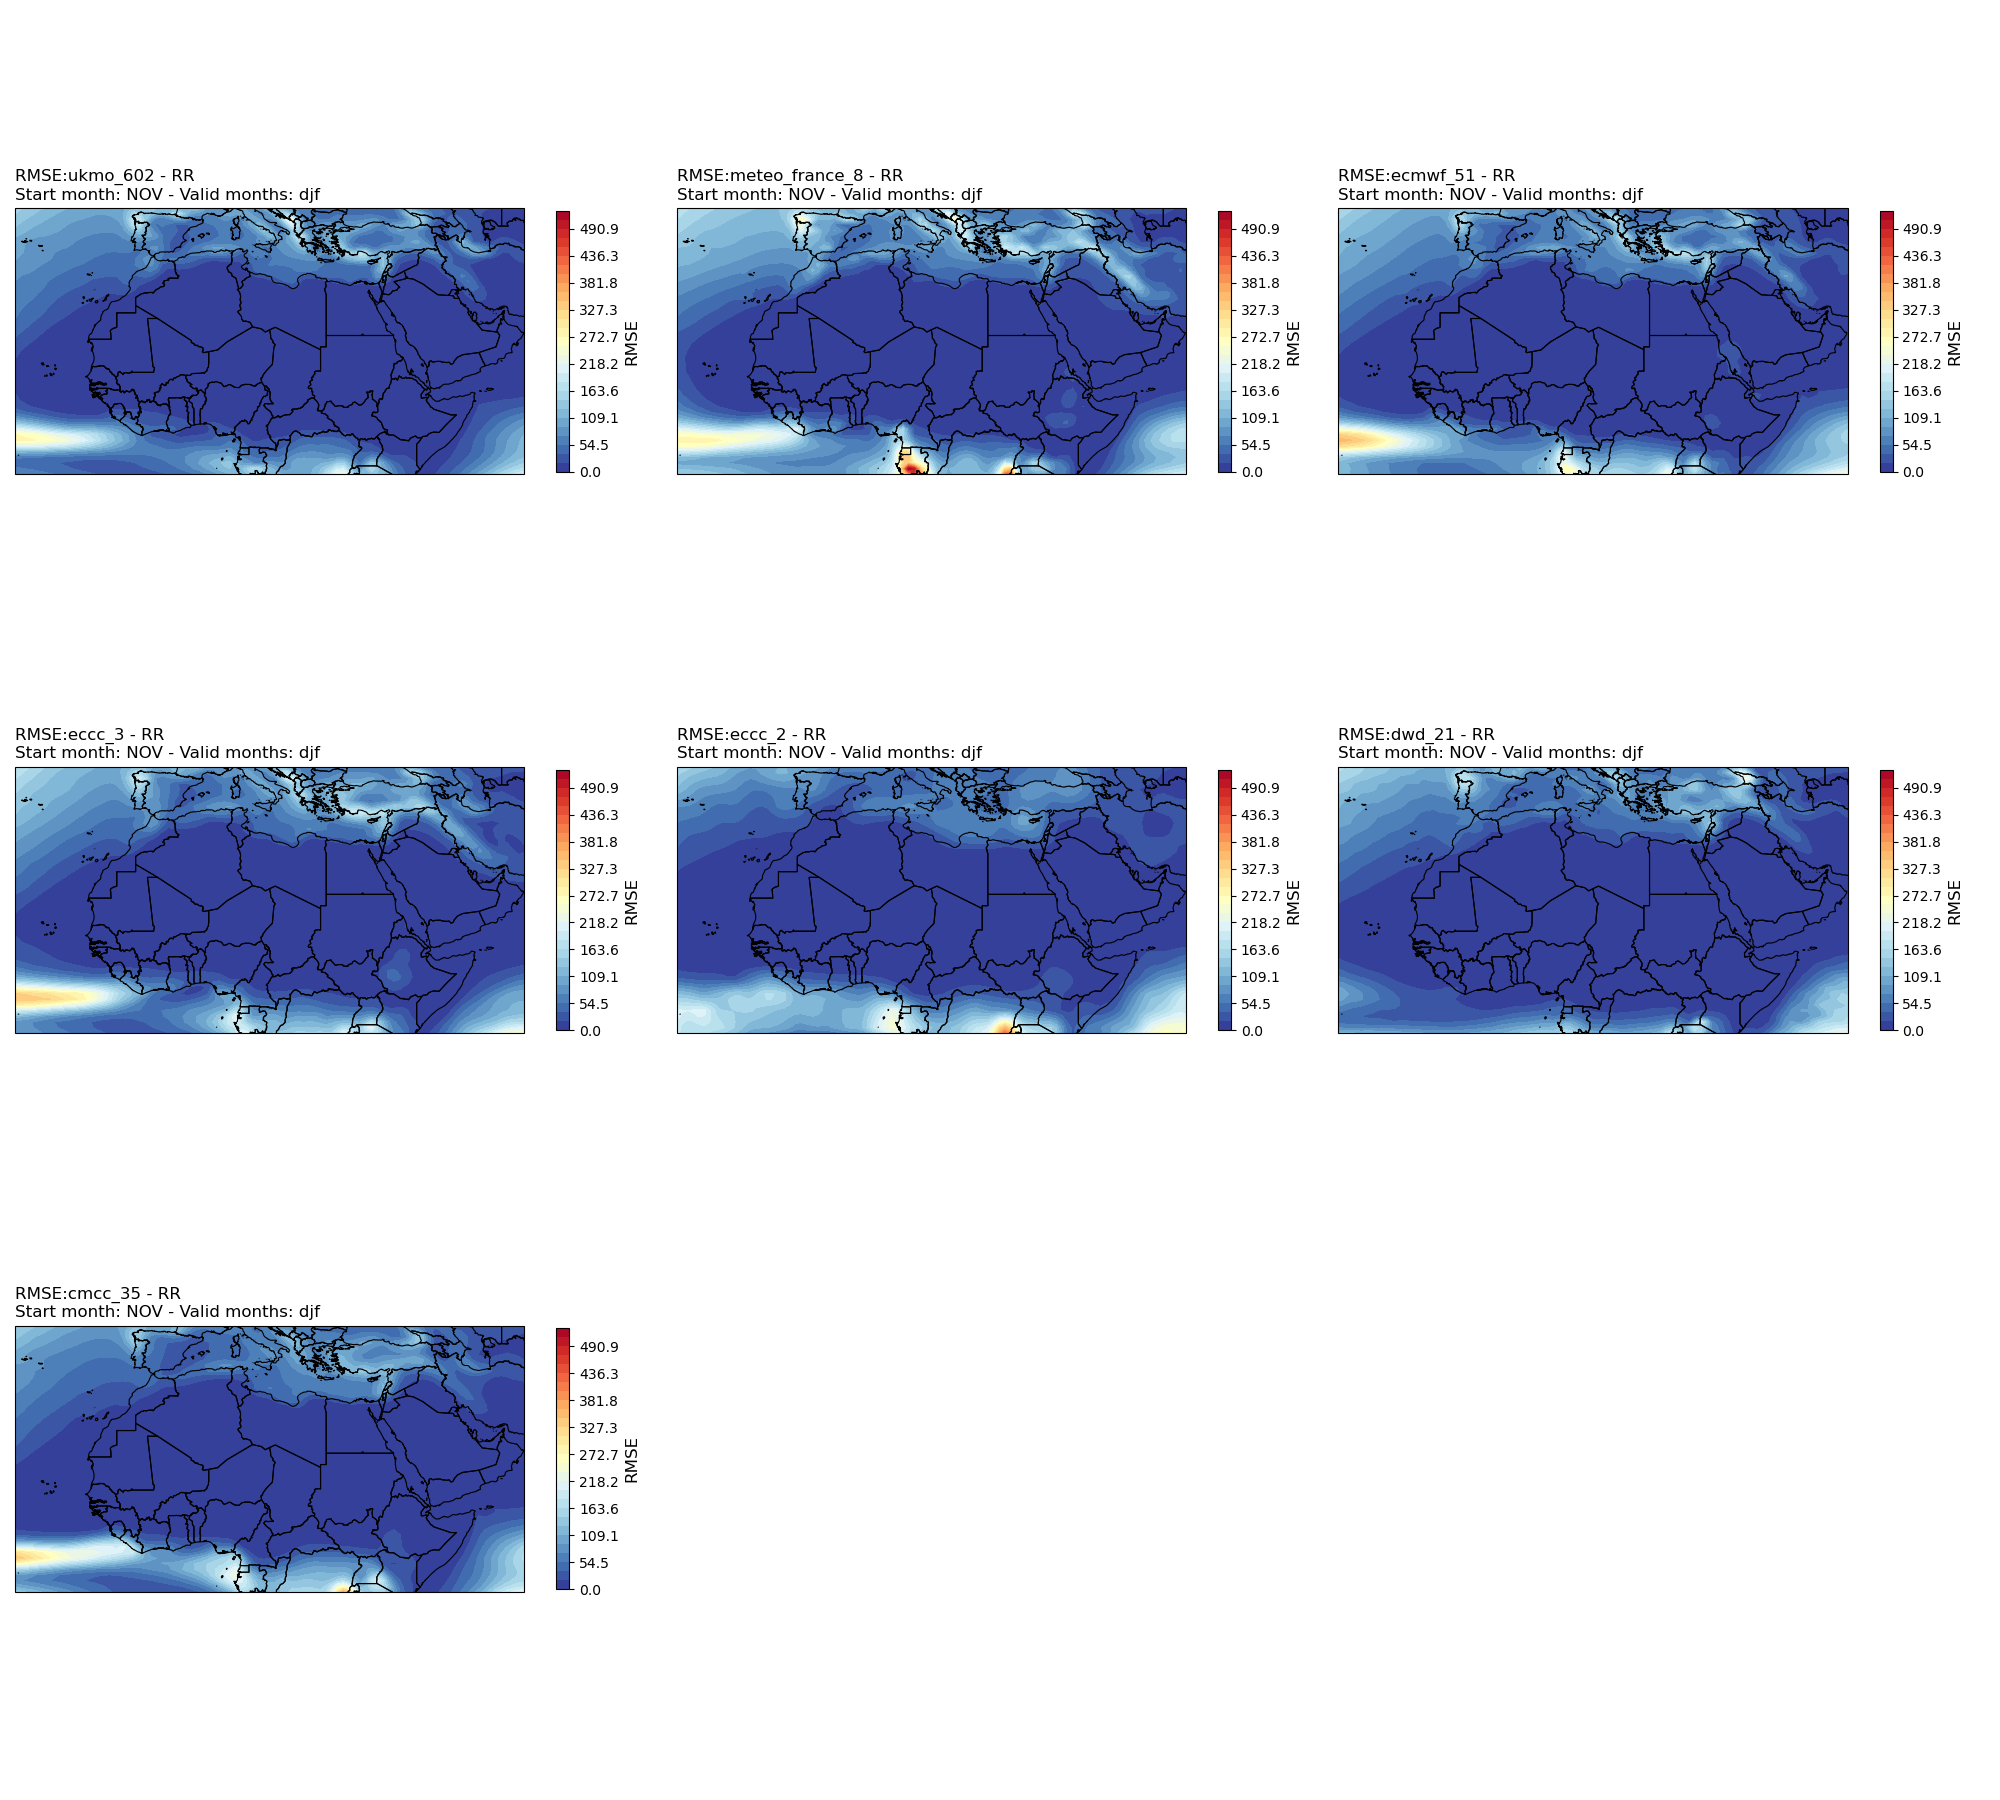
\includegraphics[scale=0.3]{plots/det/rmse/rmse_djf_RR.png}
\caption{3-months Rolling mean of RMSE in MENA Region for all centers DJF in mm}
\end{figure}

\begin{figure}[H]
\centering
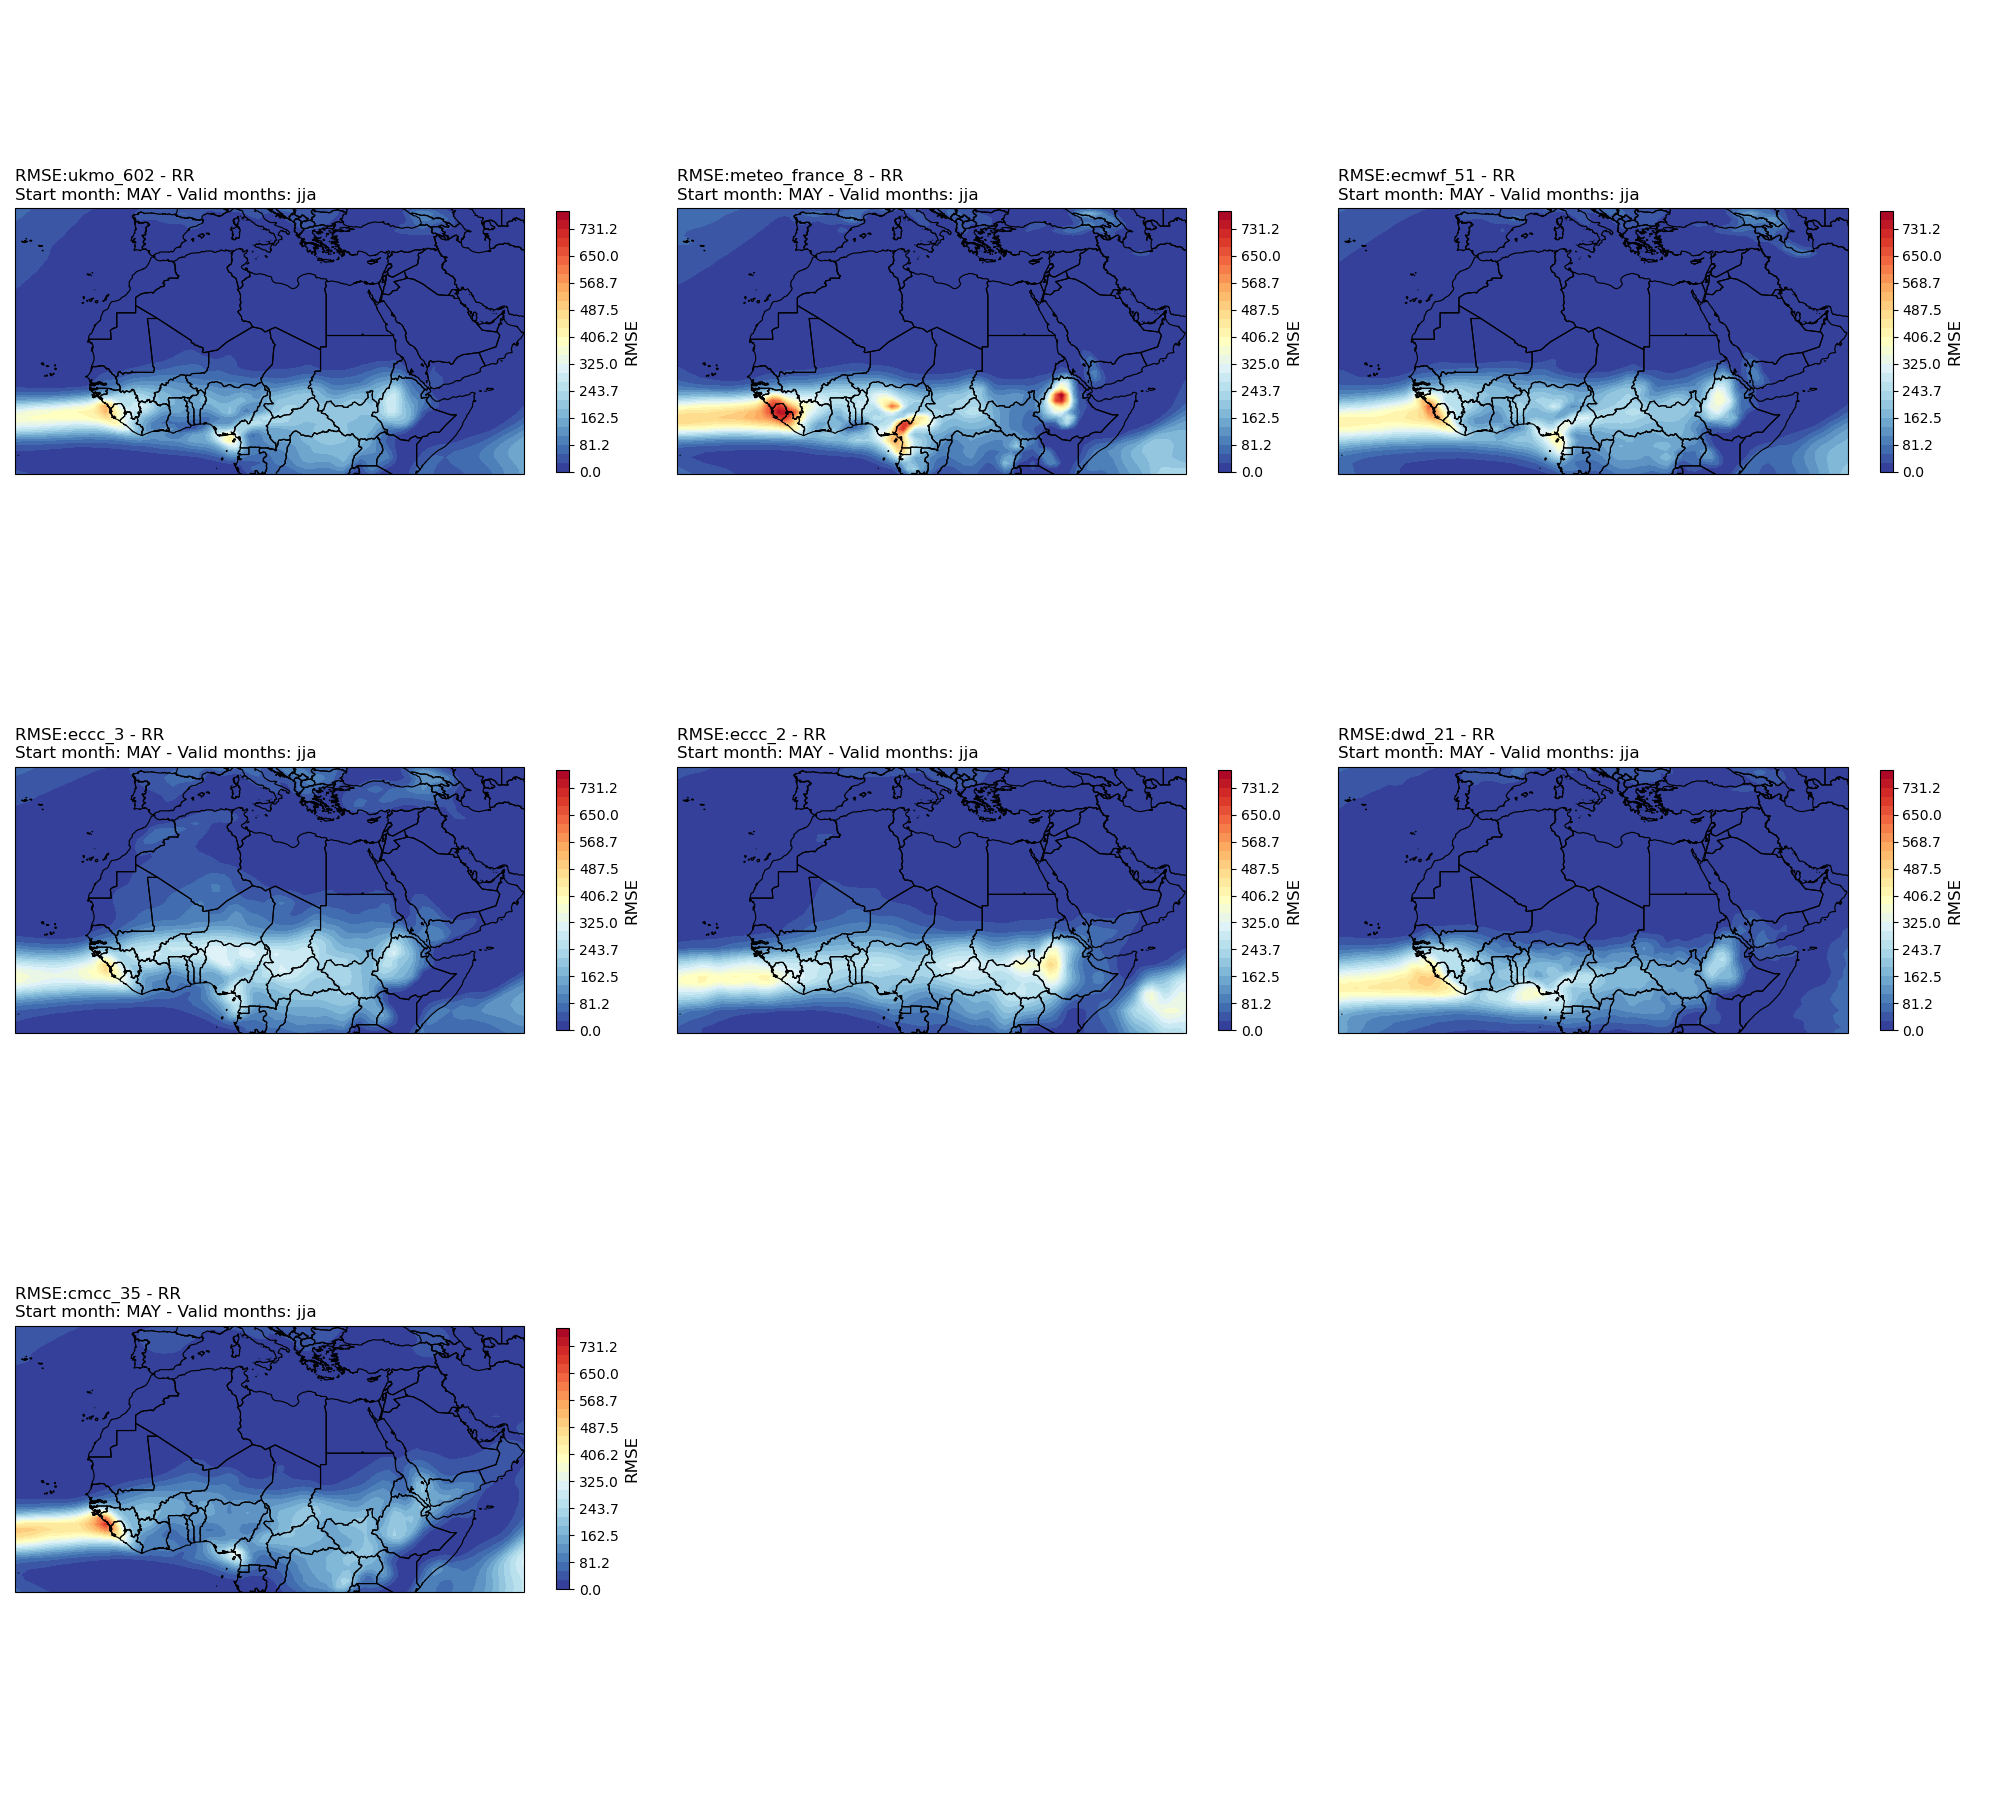
\includegraphics[scale=0.3]{plots/det/rmse/rmse_jja_RR.png}
\caption{3-months Rolling mean of RMSE in MENA Region for all centers JJA in mm}
\end{figure}

also for the spacial dimension, the RMSE stay stable and exhibit moderate performance for all centers. Thus, all models have almost the same skill and they are consistent with each other.

\begin{figure}[H]
\centering
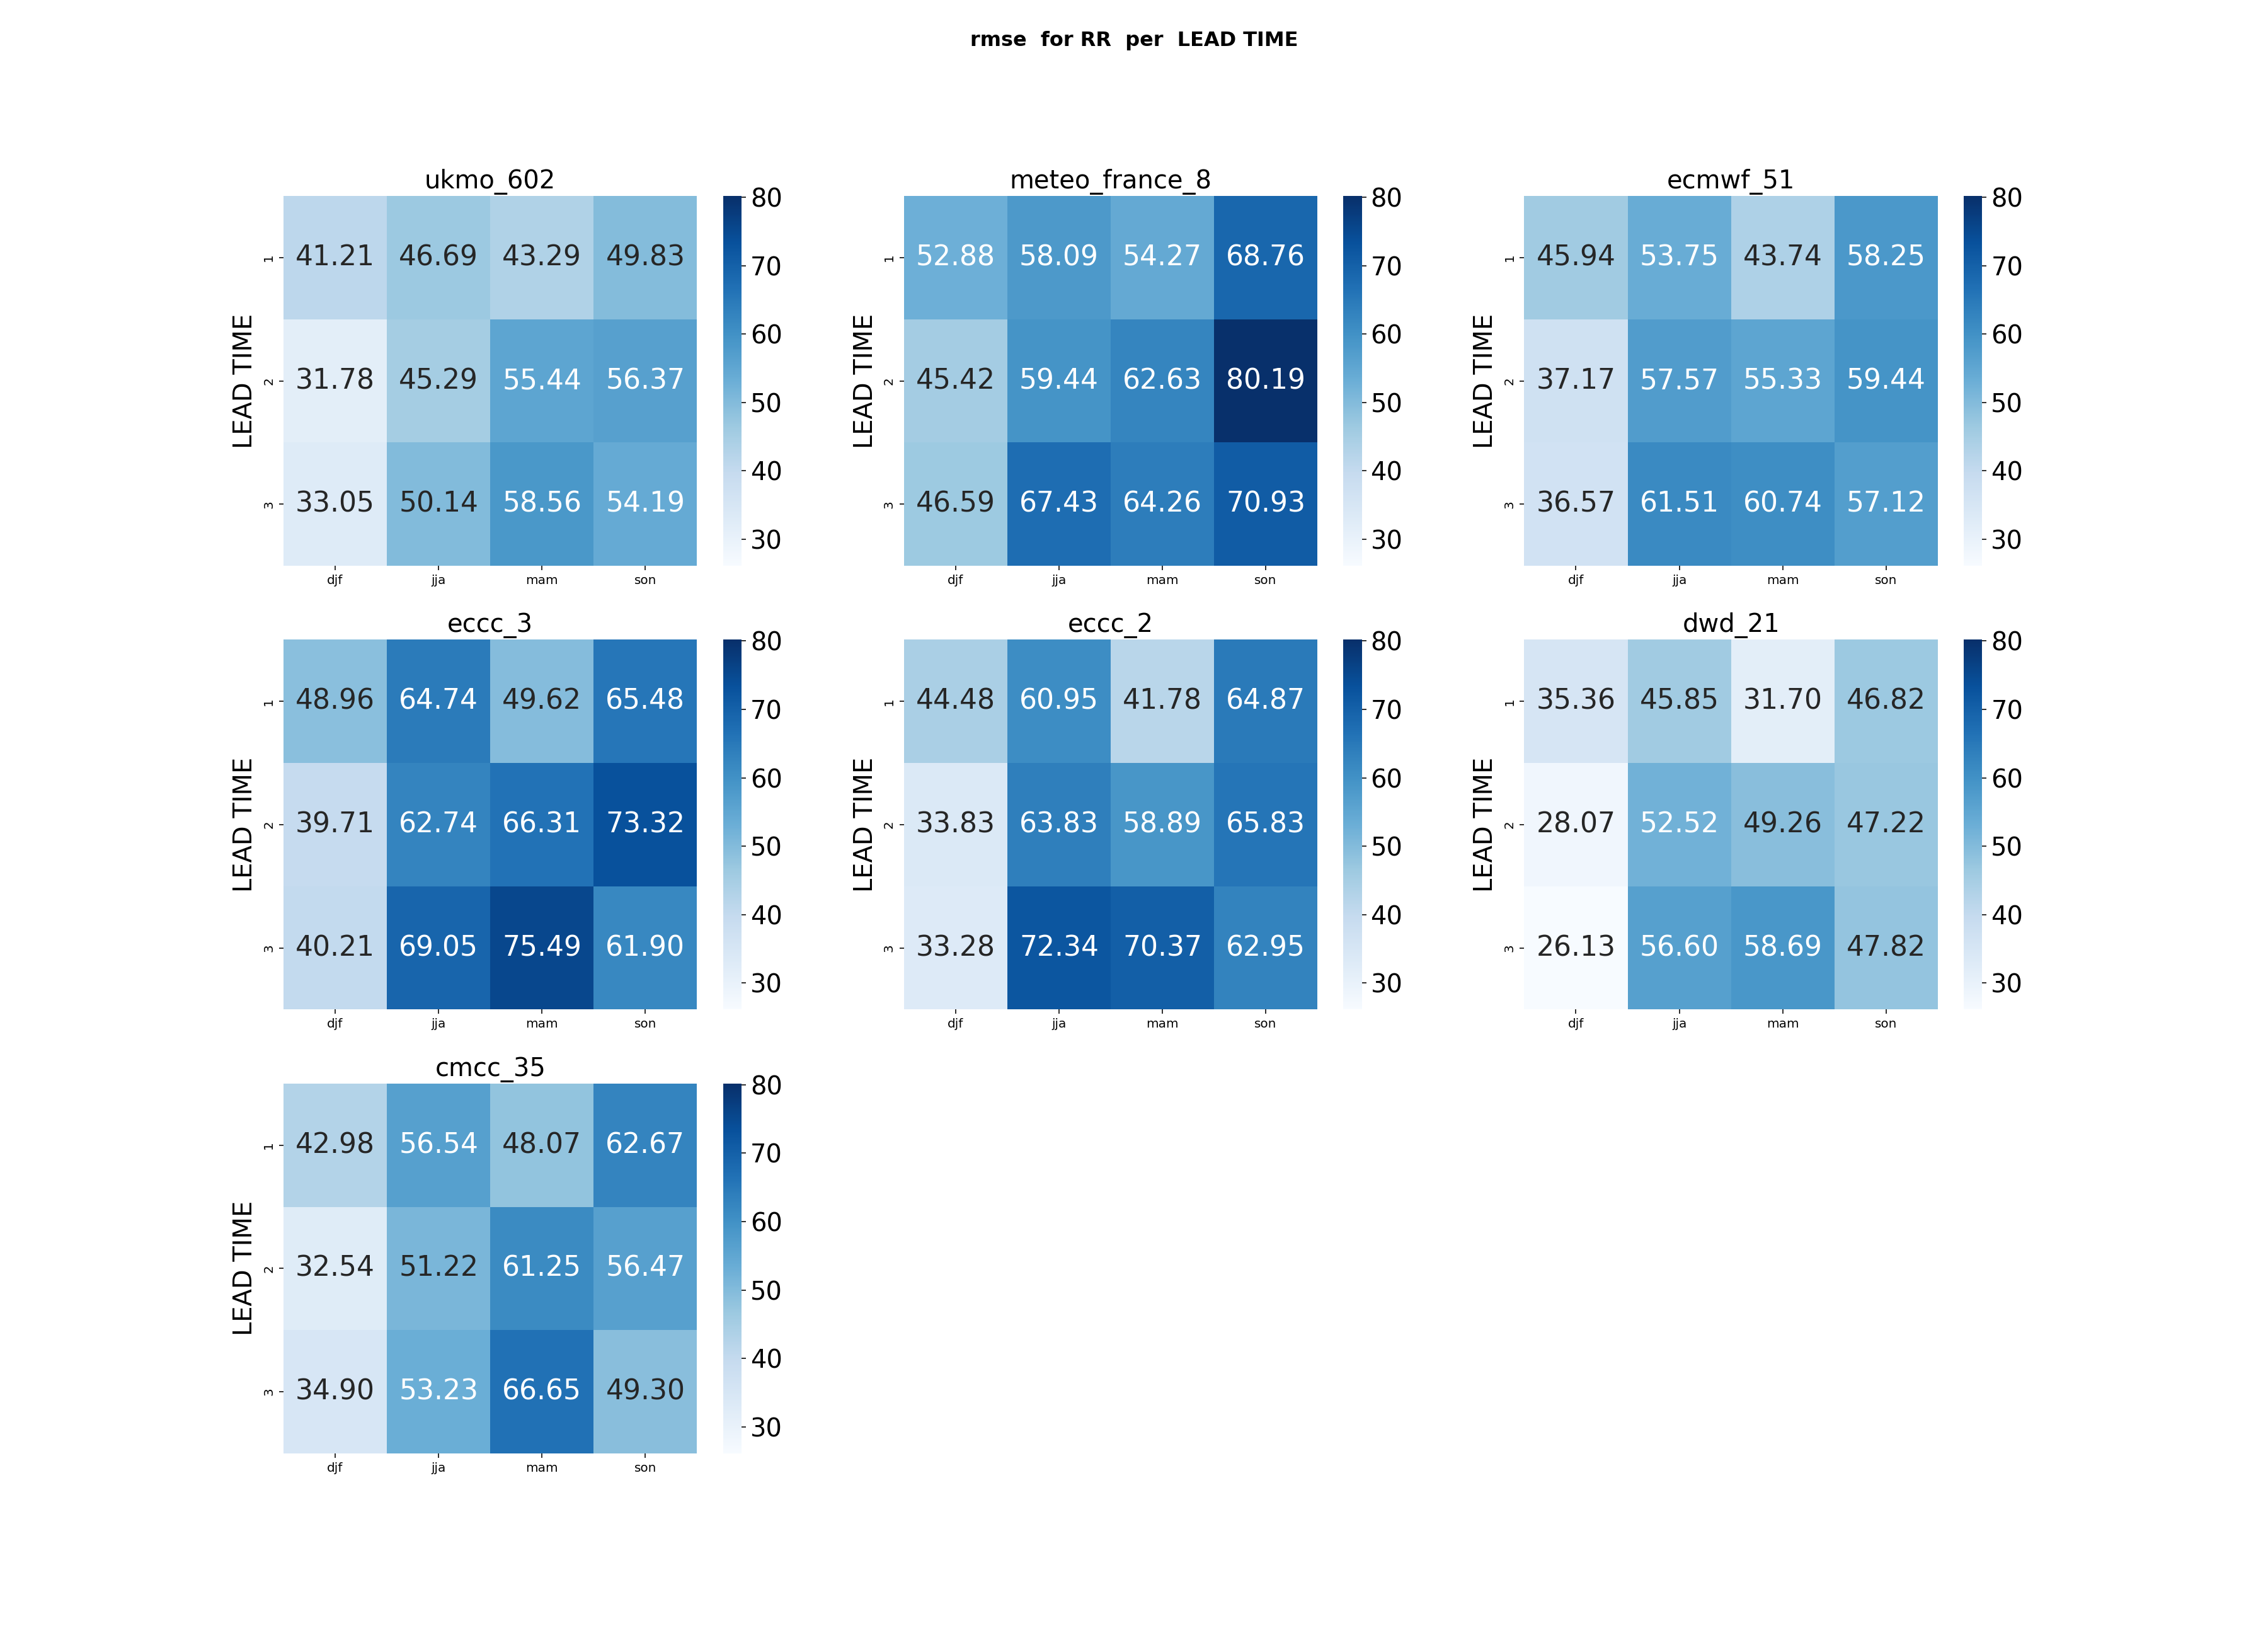
\includegraphics[scale=0.3]{plots/det/rmse/rmse_RR_mena.png}
\caption{heatmap of RMSE For RR in mm}
\end{figure}


\subsubsection{Coefficient of Determination (\( R^2 \))}
for precipitation, the R-SQUARED is very low, the maximum value is less than 0.1. However, the ecmwf is the best in term of R-SQUARED. for DJF,JJA and MAM the highest performance is in the first Lead-time, and it decrease along time, But for SON the best score is in the second Lead-time for all centers.
\begin{figure}[H]
	\centering
	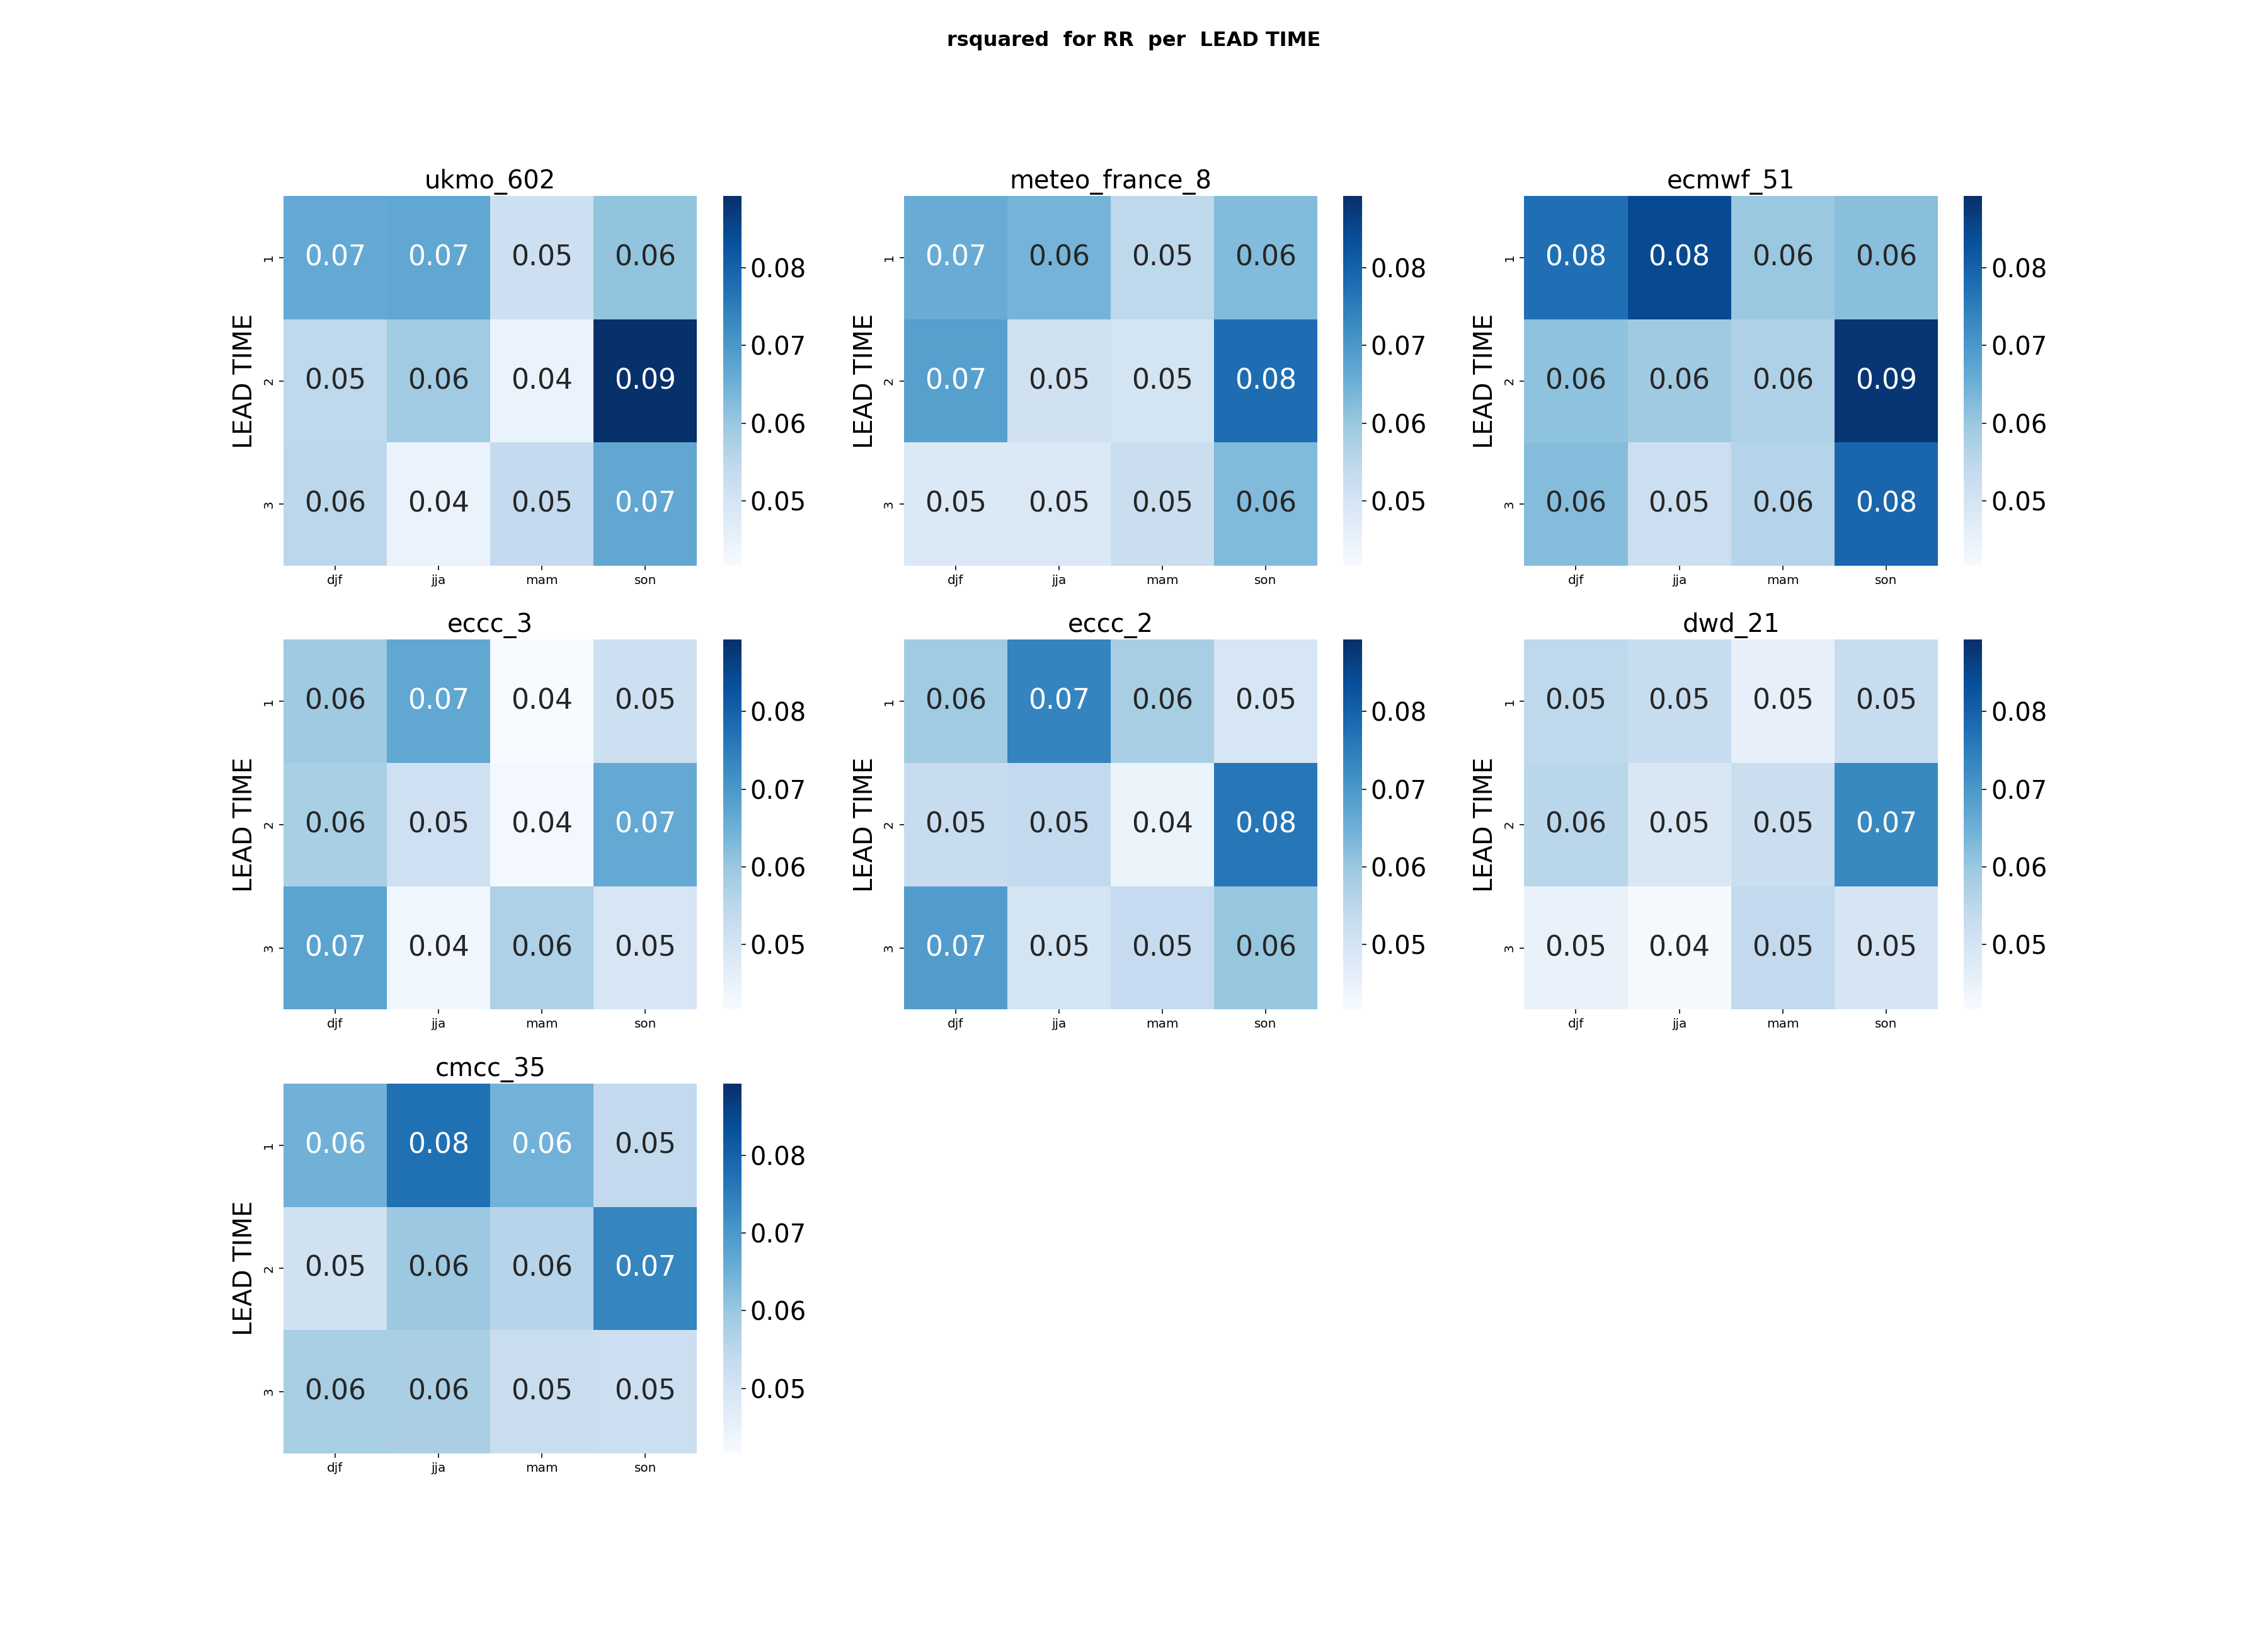
\includegraphics[scale=0.25]{plots/det/rsquared/rsquared_RR_mena.png}
	\caption{The Heatmap of rsquared for Precipitations in the mena region for every period \textbf{\textit{(1 for perfect RSQUARED)} }}
\end{figure}


\begin{figure}[H]
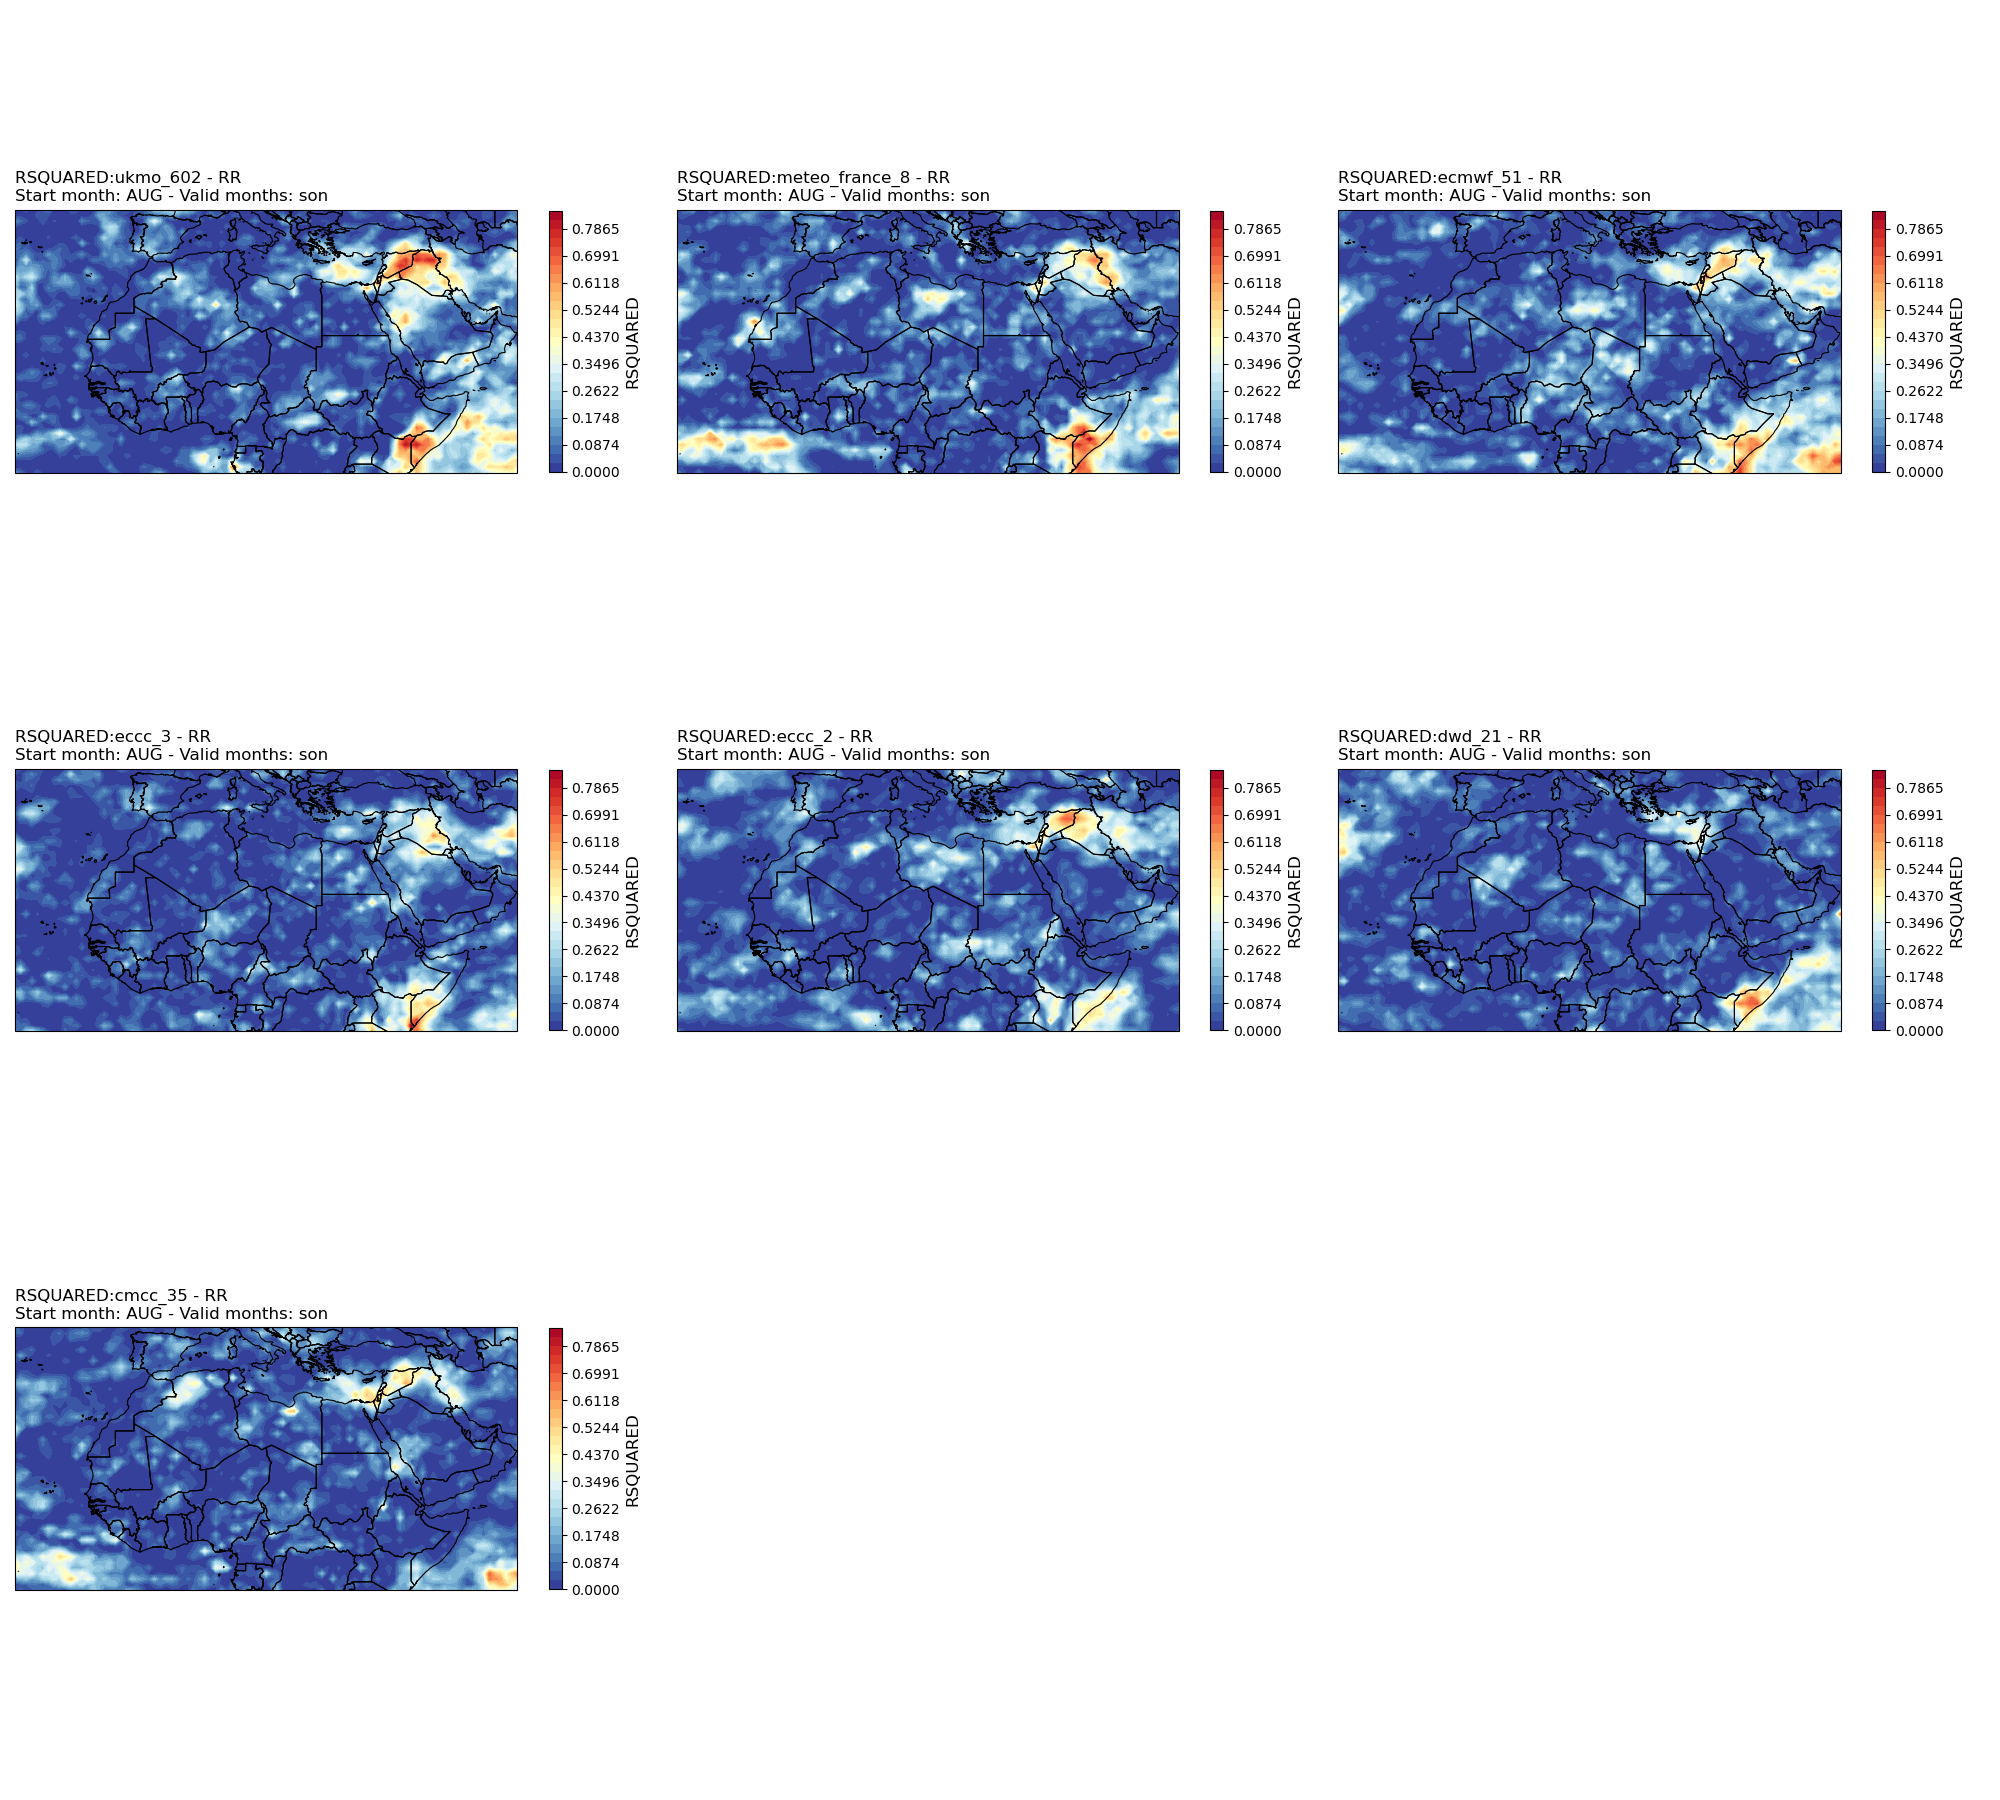
\includegraphics[scale=0.3]{plots/det/rsquared/rsquared_son_RR.png}
\caption{3-months Rolling mean of RSQUARED in MENA Region for all centers SON}
\end{figure}

there is some isolated zones where the r-squared is good especially in Syria, Irak, Jordan ,Palestine  and East Africa, this high performance is observed in all centers. For the rest of the MENA region the performance is very bad with score near to 0. Hence, there is no constant pattern for the R-SQUARED, the spacial variation is very high for all centers.


\subsection{Probabilistic Evaluation Metrics}

\subsubsection{The Brier Score (BS)}

\begin{figure}[H]
    \centering
    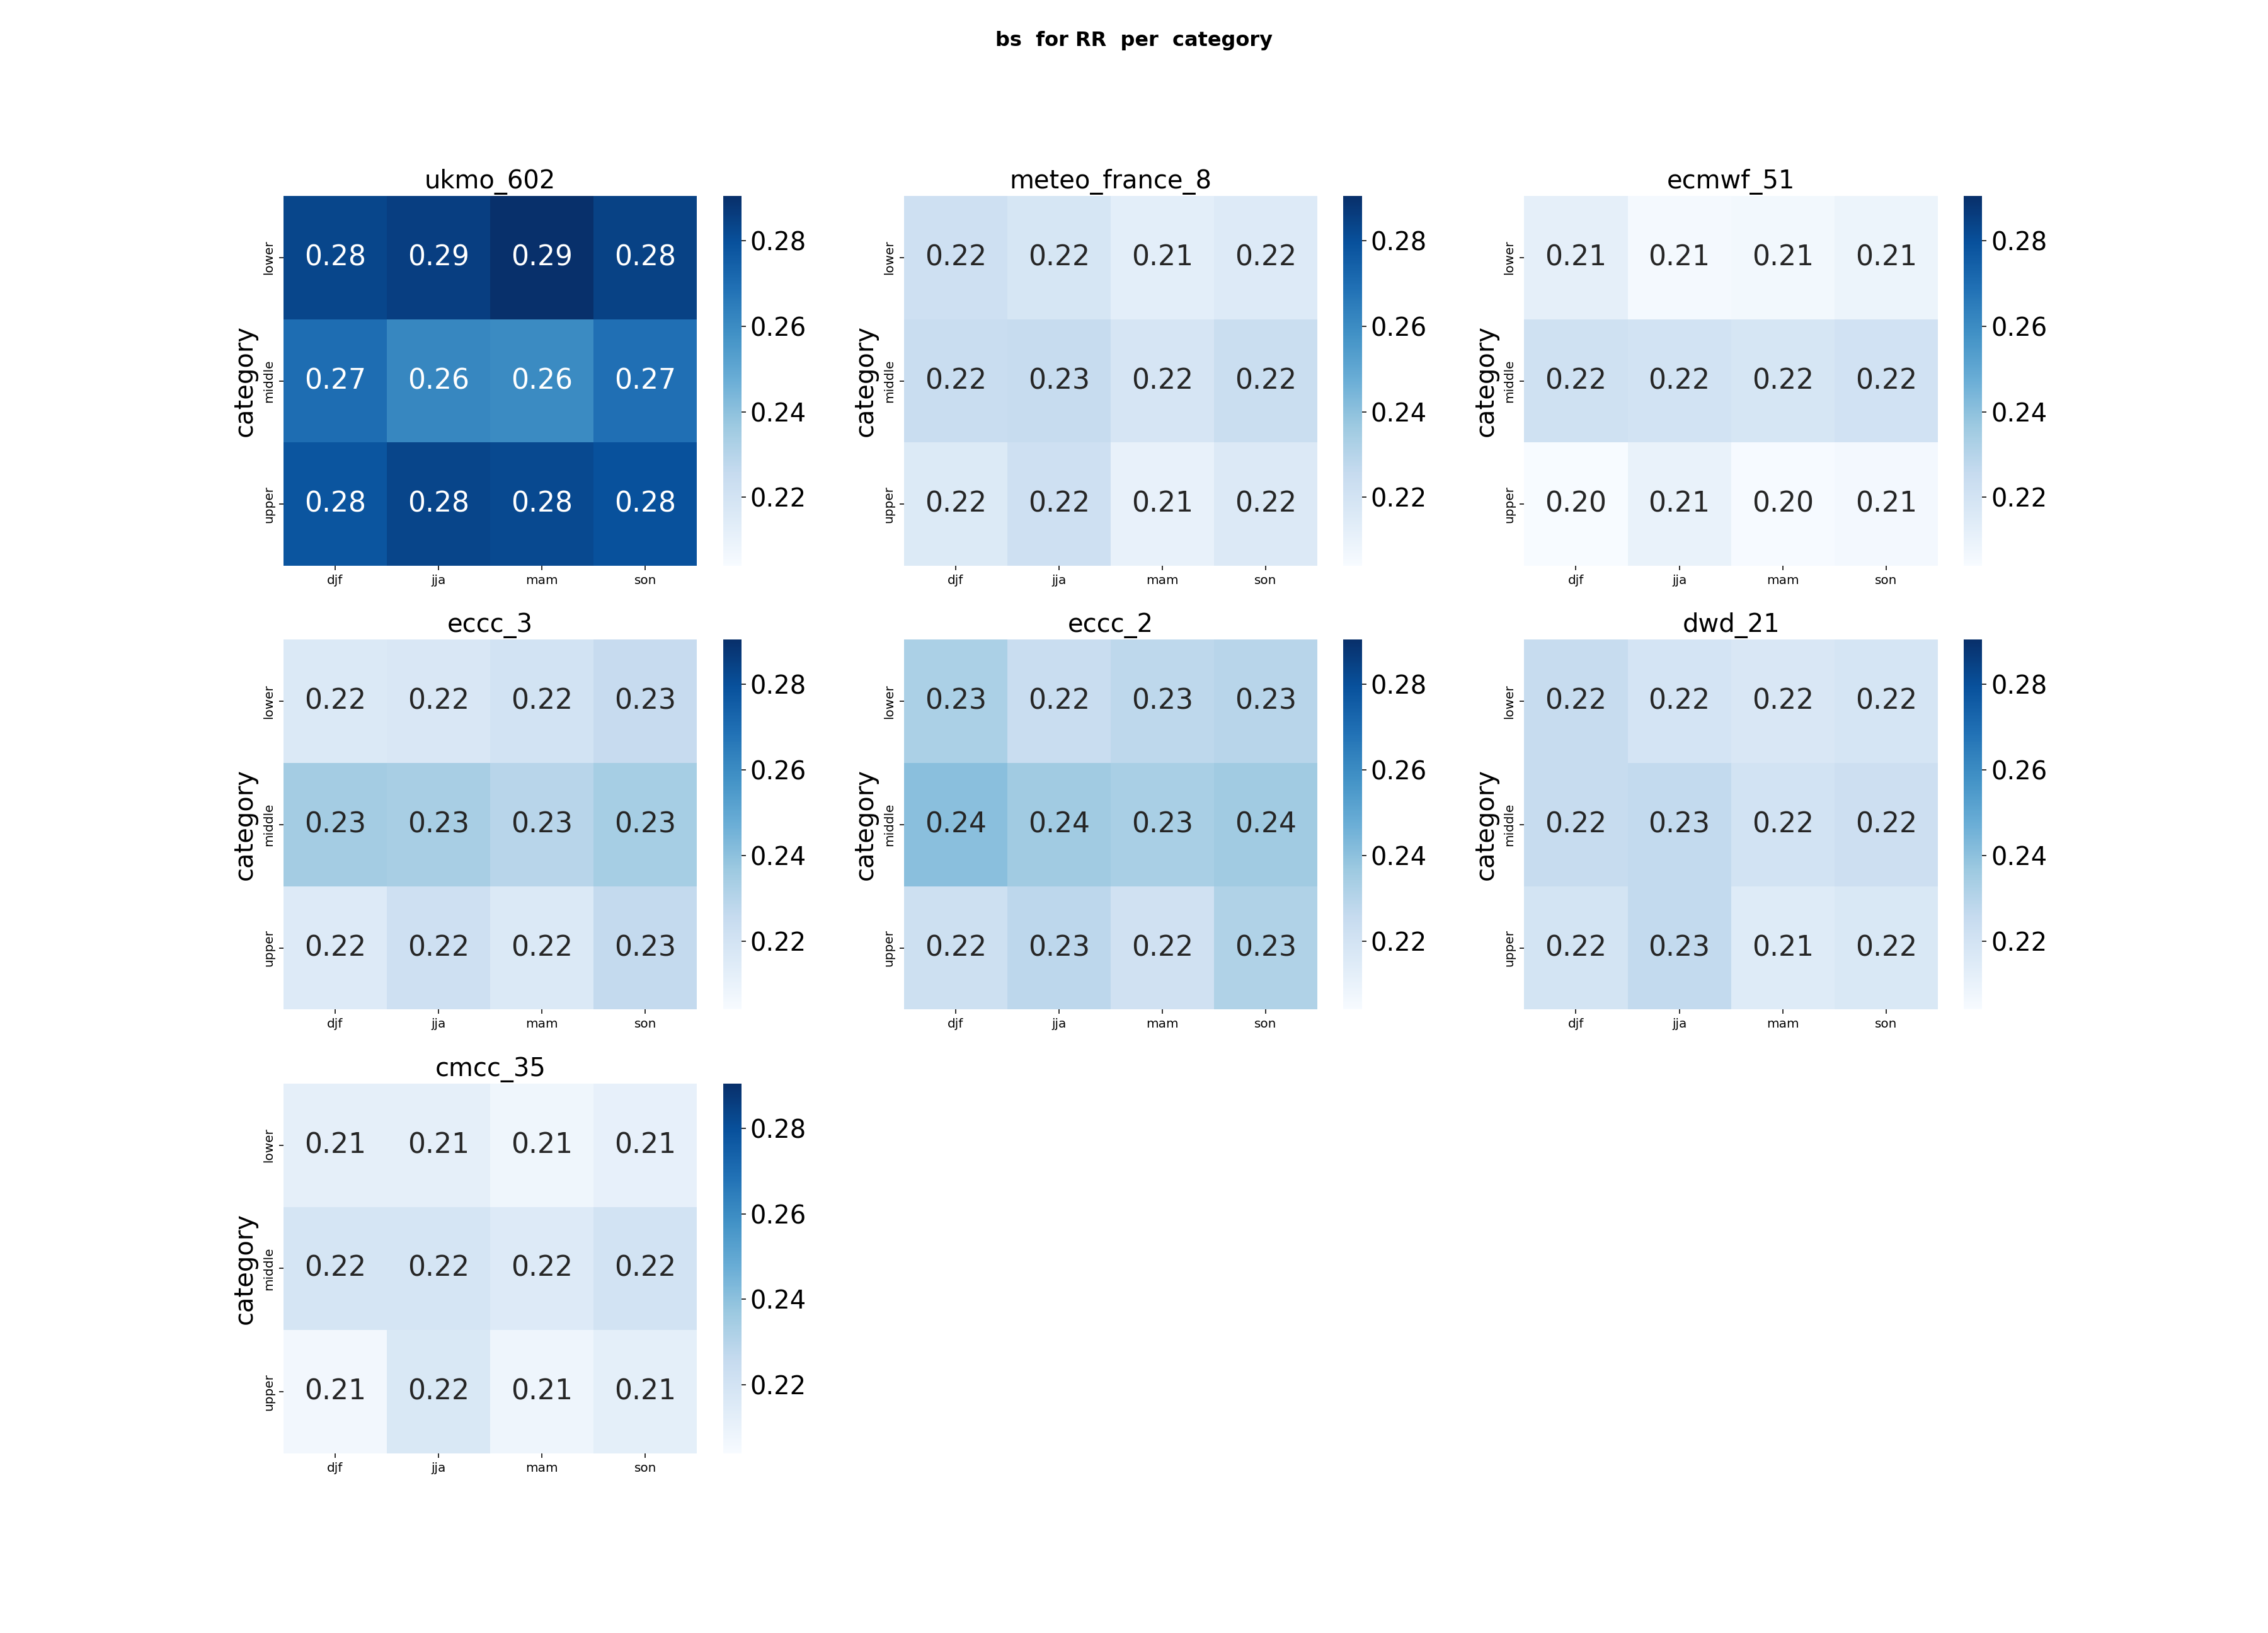
\includegraphics[scale=0.25]{plots/prob/bs/bs_RR_category.png}
    \caption{The Heatmap of Brier Score for each category  . \textbf{\textit{(0 represents perfect BS)}}}
\end{figure}

for the analysis per category, we can see in the figure above that all centers exhibit good performance in term of Brier Score except the UMKO that shows moderate BS. Overall, the middle tercile shows lower performance (higher Brier Score) for all centers. 
the figure below shows the analysis per lead-time. the same result is found, but the \textbf{\textit{ECMWF,METEO-FRANCE and CMCC-35}} are the best models in Brier Score for lead-time analysis.The performance stay stable along time which is a reliable signal. Despite the UKMO have the lower performance, it stays close to the other centers, the difference isn't so wide. 
In general, the performance stays stable over category, lead-time and space.


\begin{figure}[H]
    \centering
    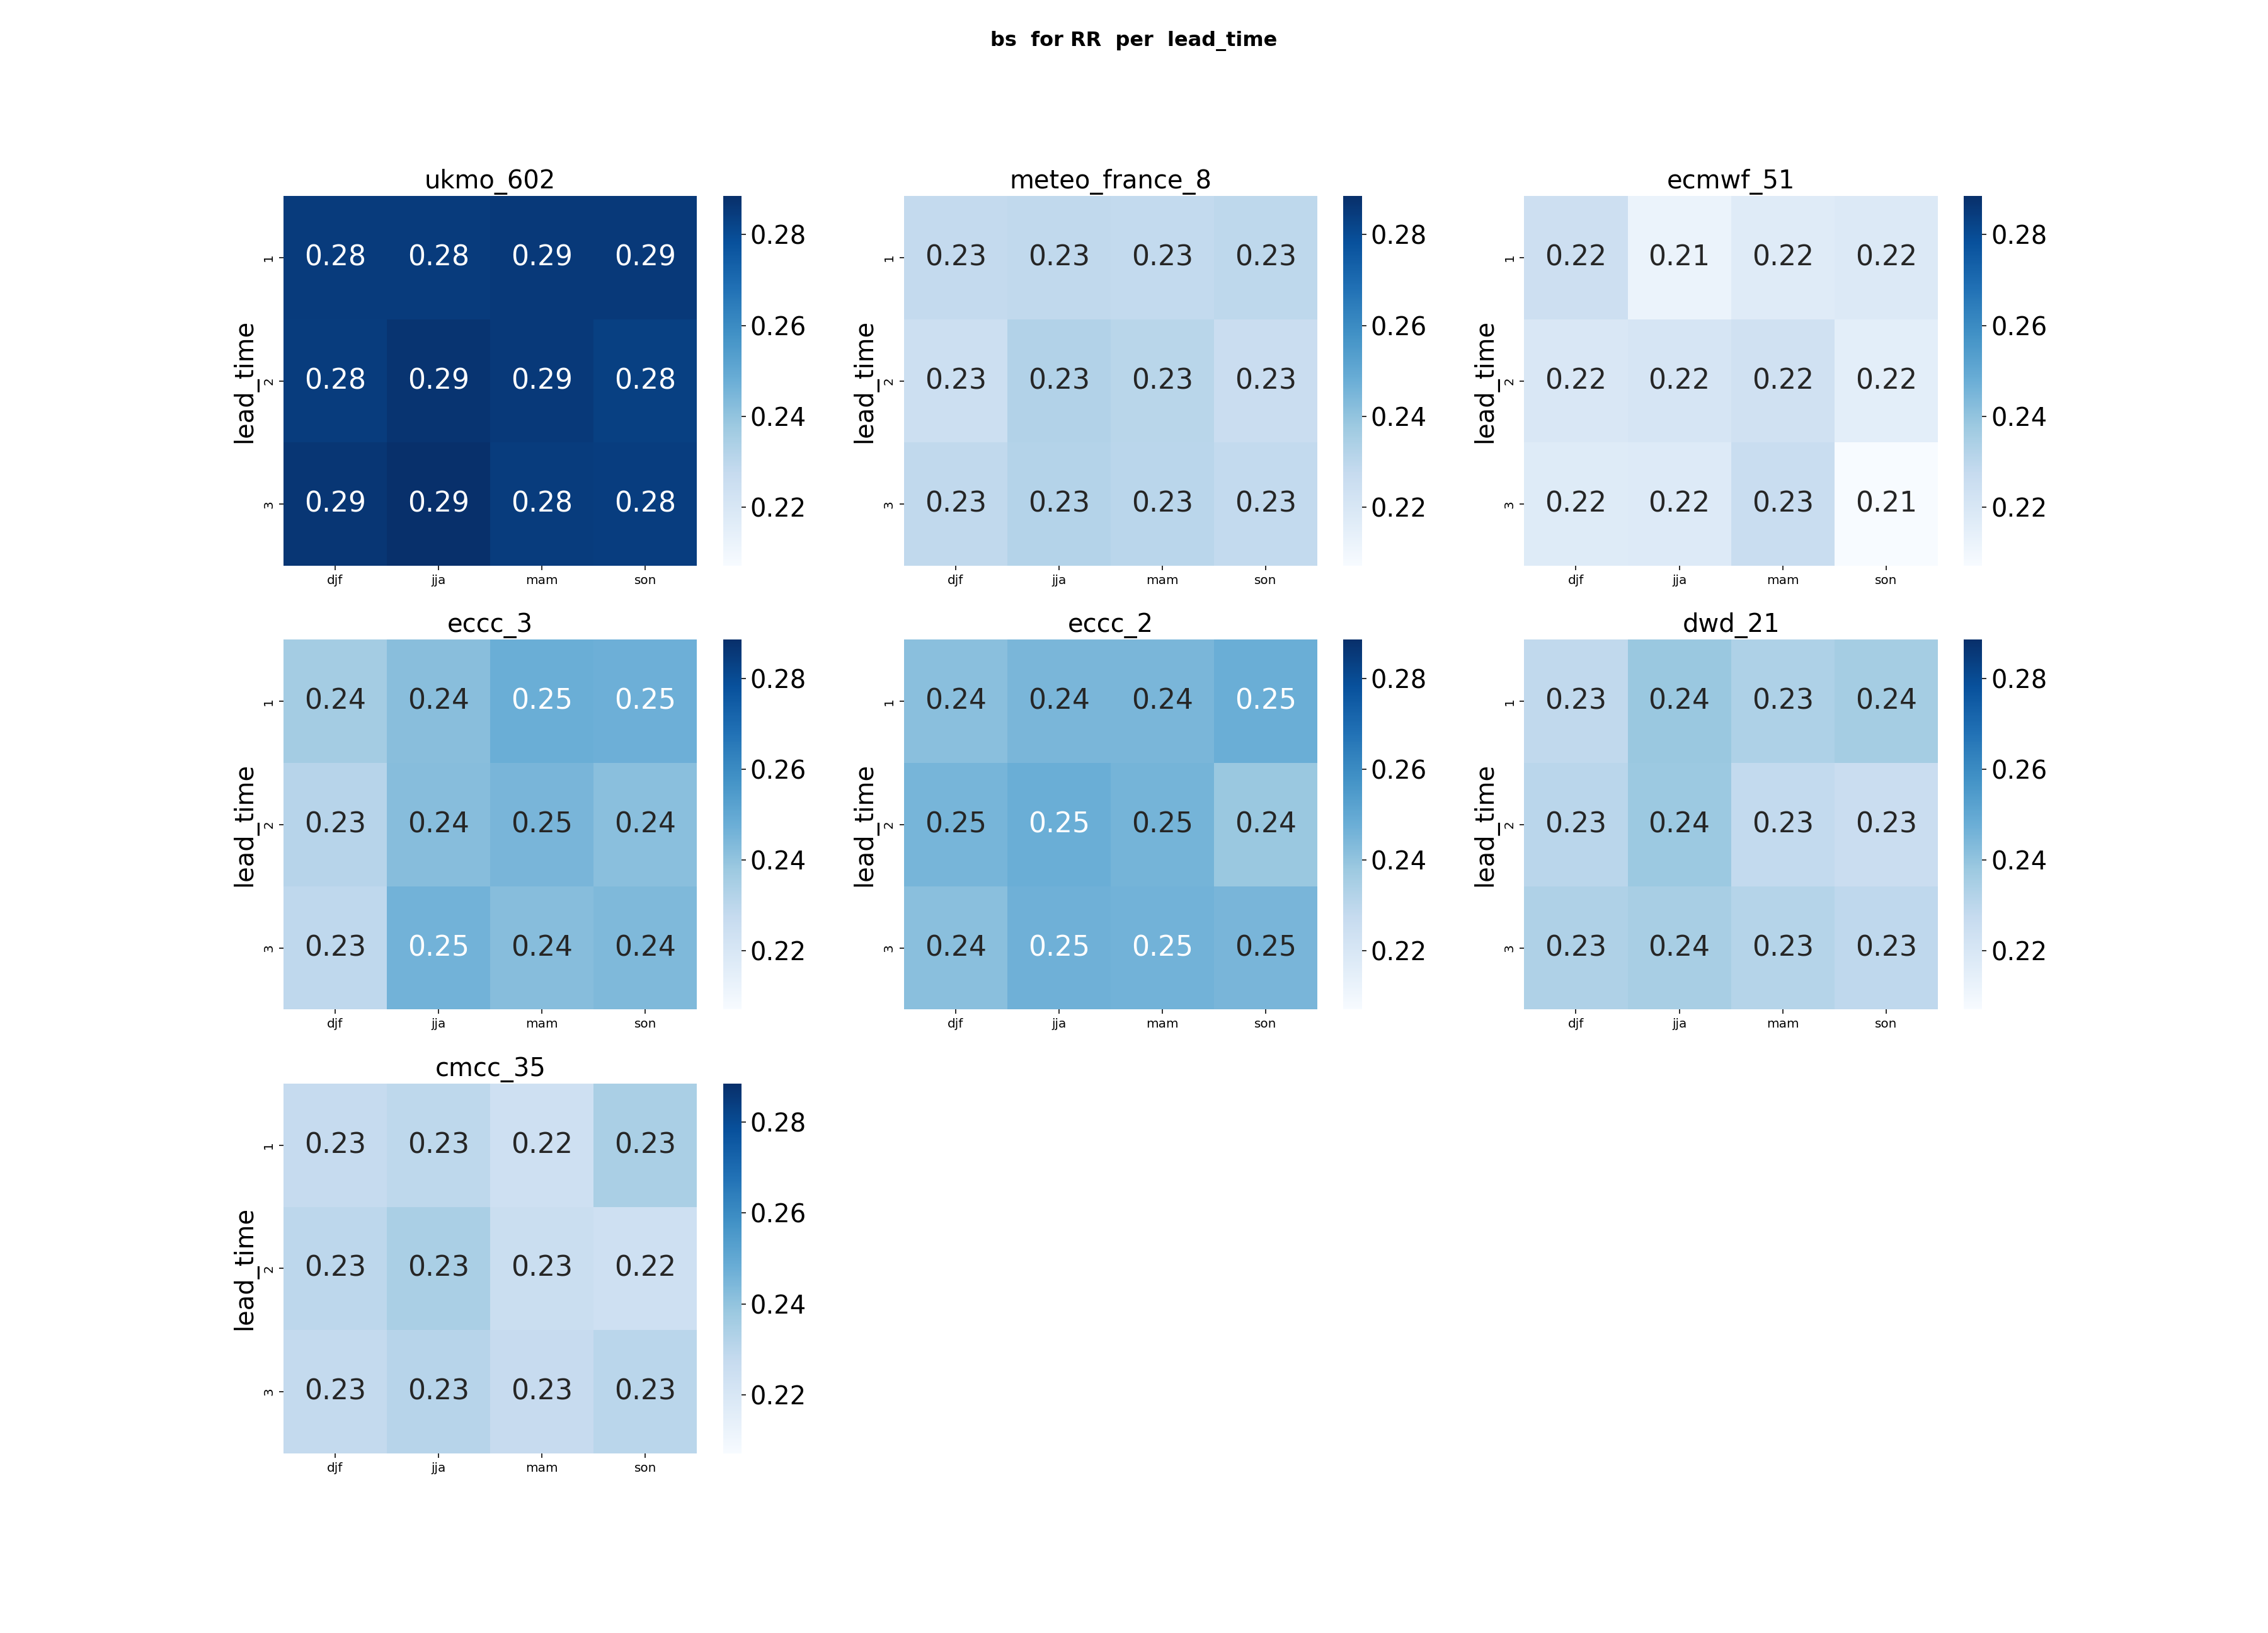
\includegraphics[scale=0.25]{plots/prob/bs/bs_RR_lead_time.png}
    \caption{The Heatmap of Brier Score for lead-time. \textbf{\textit{(0 represents perfect BS)}}}
\end{figure}


\begin{figure}[H]
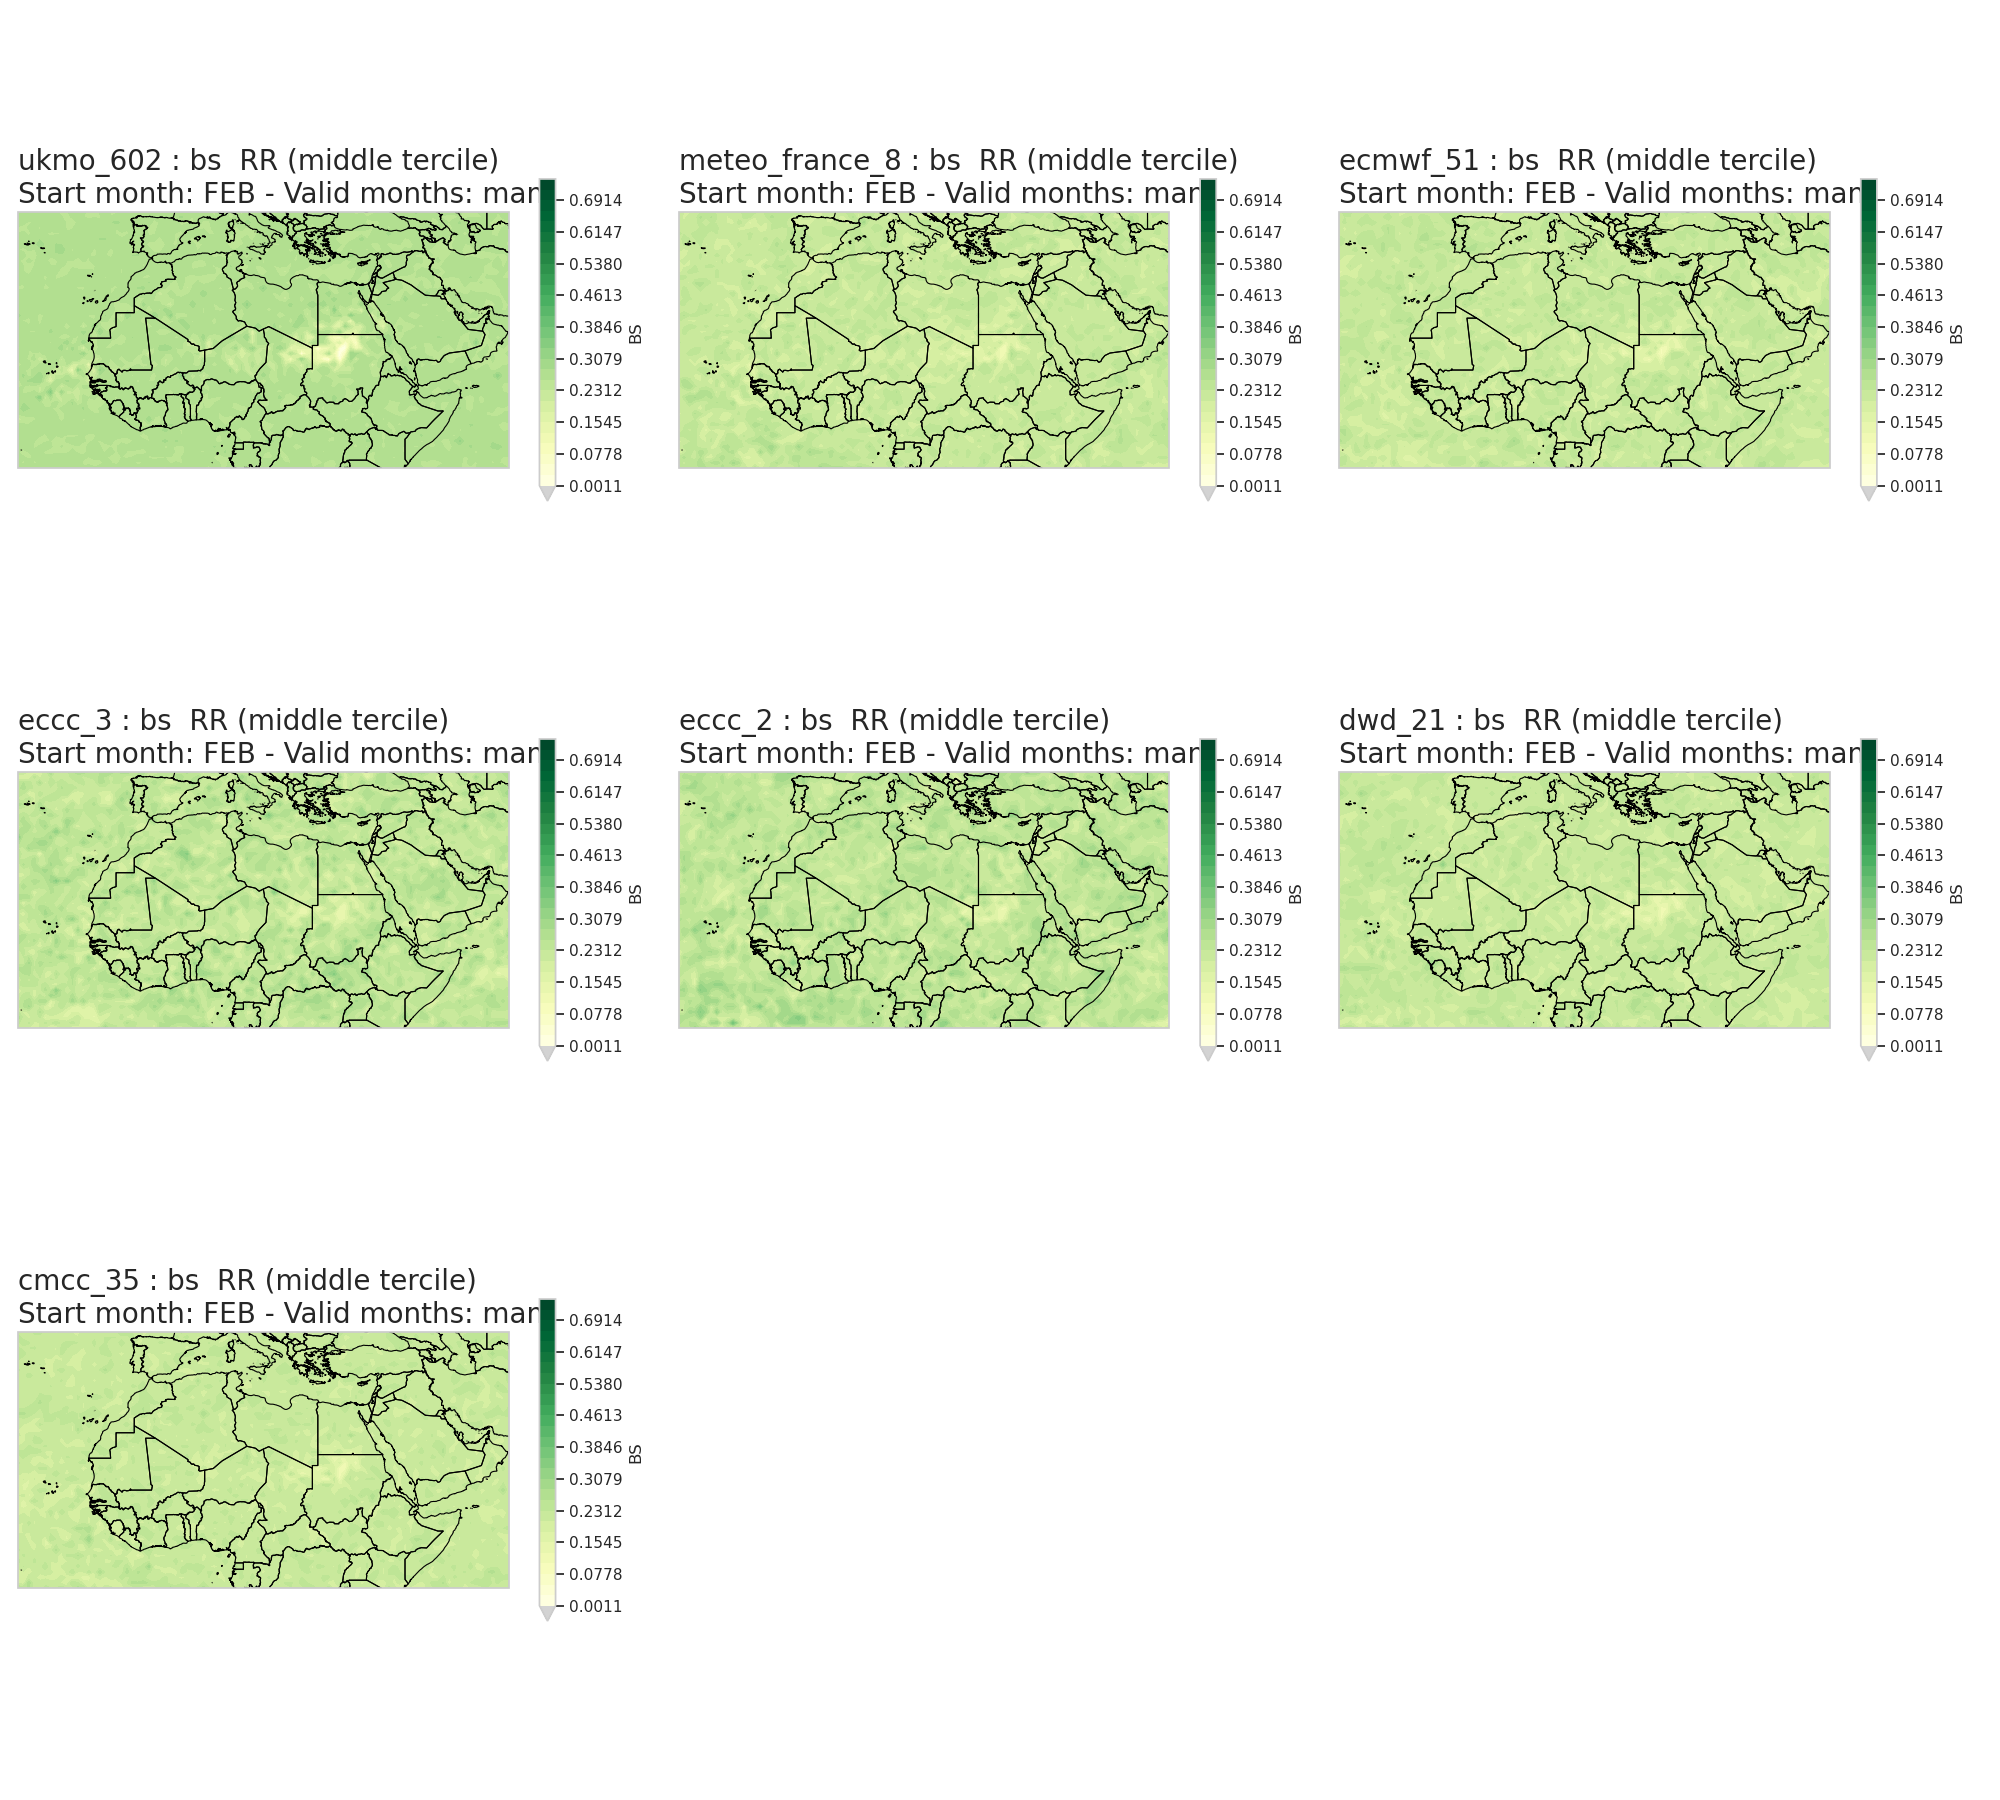
\includegraphics[scale=0.3]{plots/prob/bs/bs_mam_RR_middle.png}
\caption{3-months Rolling mean of Brier Score in MENA Region for all centers middle tercile MAM}
\end{figure}

the spacial distribution of the BS is homogeneous, the same performance across the MENA region, almost all centers perform well for all lead-times, for  tercile there is a little lower performance for the middle tercile.
Hint, for the other seasons the results are almost the same. 


\subsubsection{Reliability}

\begin{figure}[H]
    \centering
    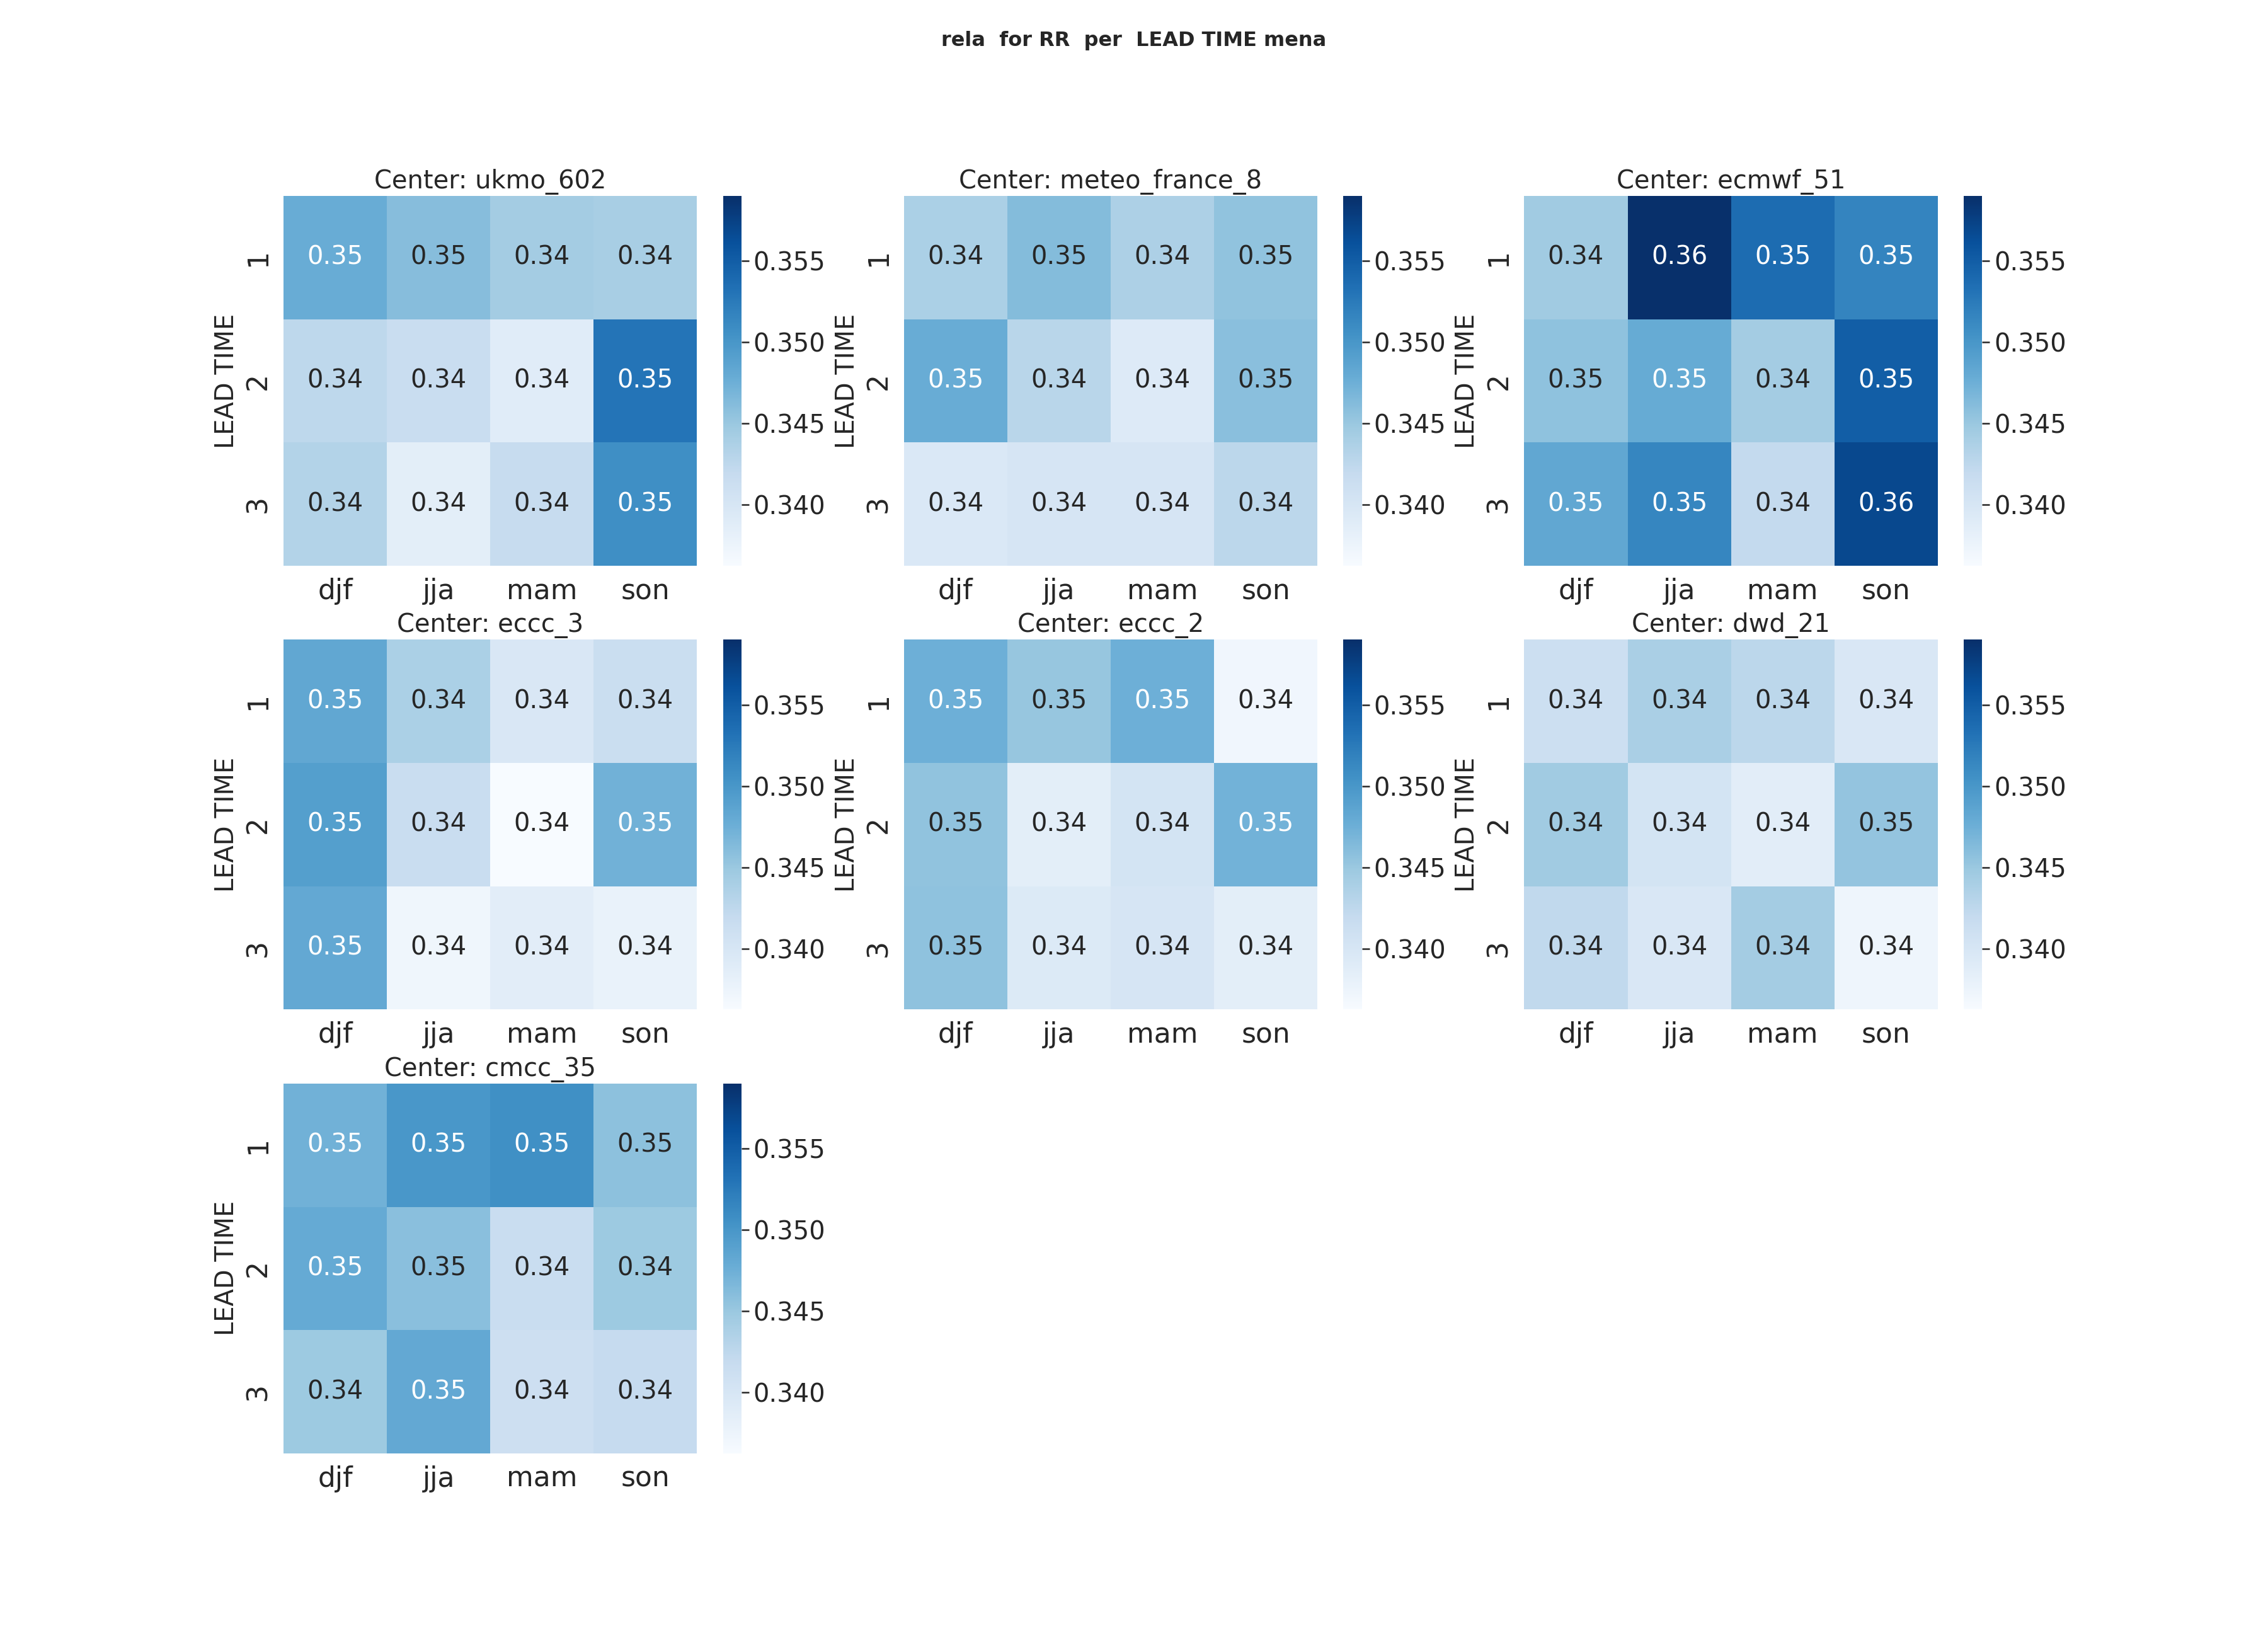
\includegraphics[scale=0.25]{plots/prob/rela/rela_RR_mena.png}
    \caption{The Reliability Score  . \textbf{\textit{(0 means perfect Reliability)}}}
\end{figure}

In the figure above, all centers demonstrate similar moderate performance in term of reliability. But deep analysis within the figure below, shows that UKMO has very bad performance, also we can distinguish three models that have the best reliability according to the reliability diagram, the centers are \textbf{\textit{ECMWF,CMCC and METEO-FRANCE}}. Hence,all centers give similar description of the reliability, also the stability along lead-time is a good indicator despite of the moderate results (0.3), we can rely on the models cited above because of the acceptable results and the stability along time.

\begin{figure}[H]
\centering
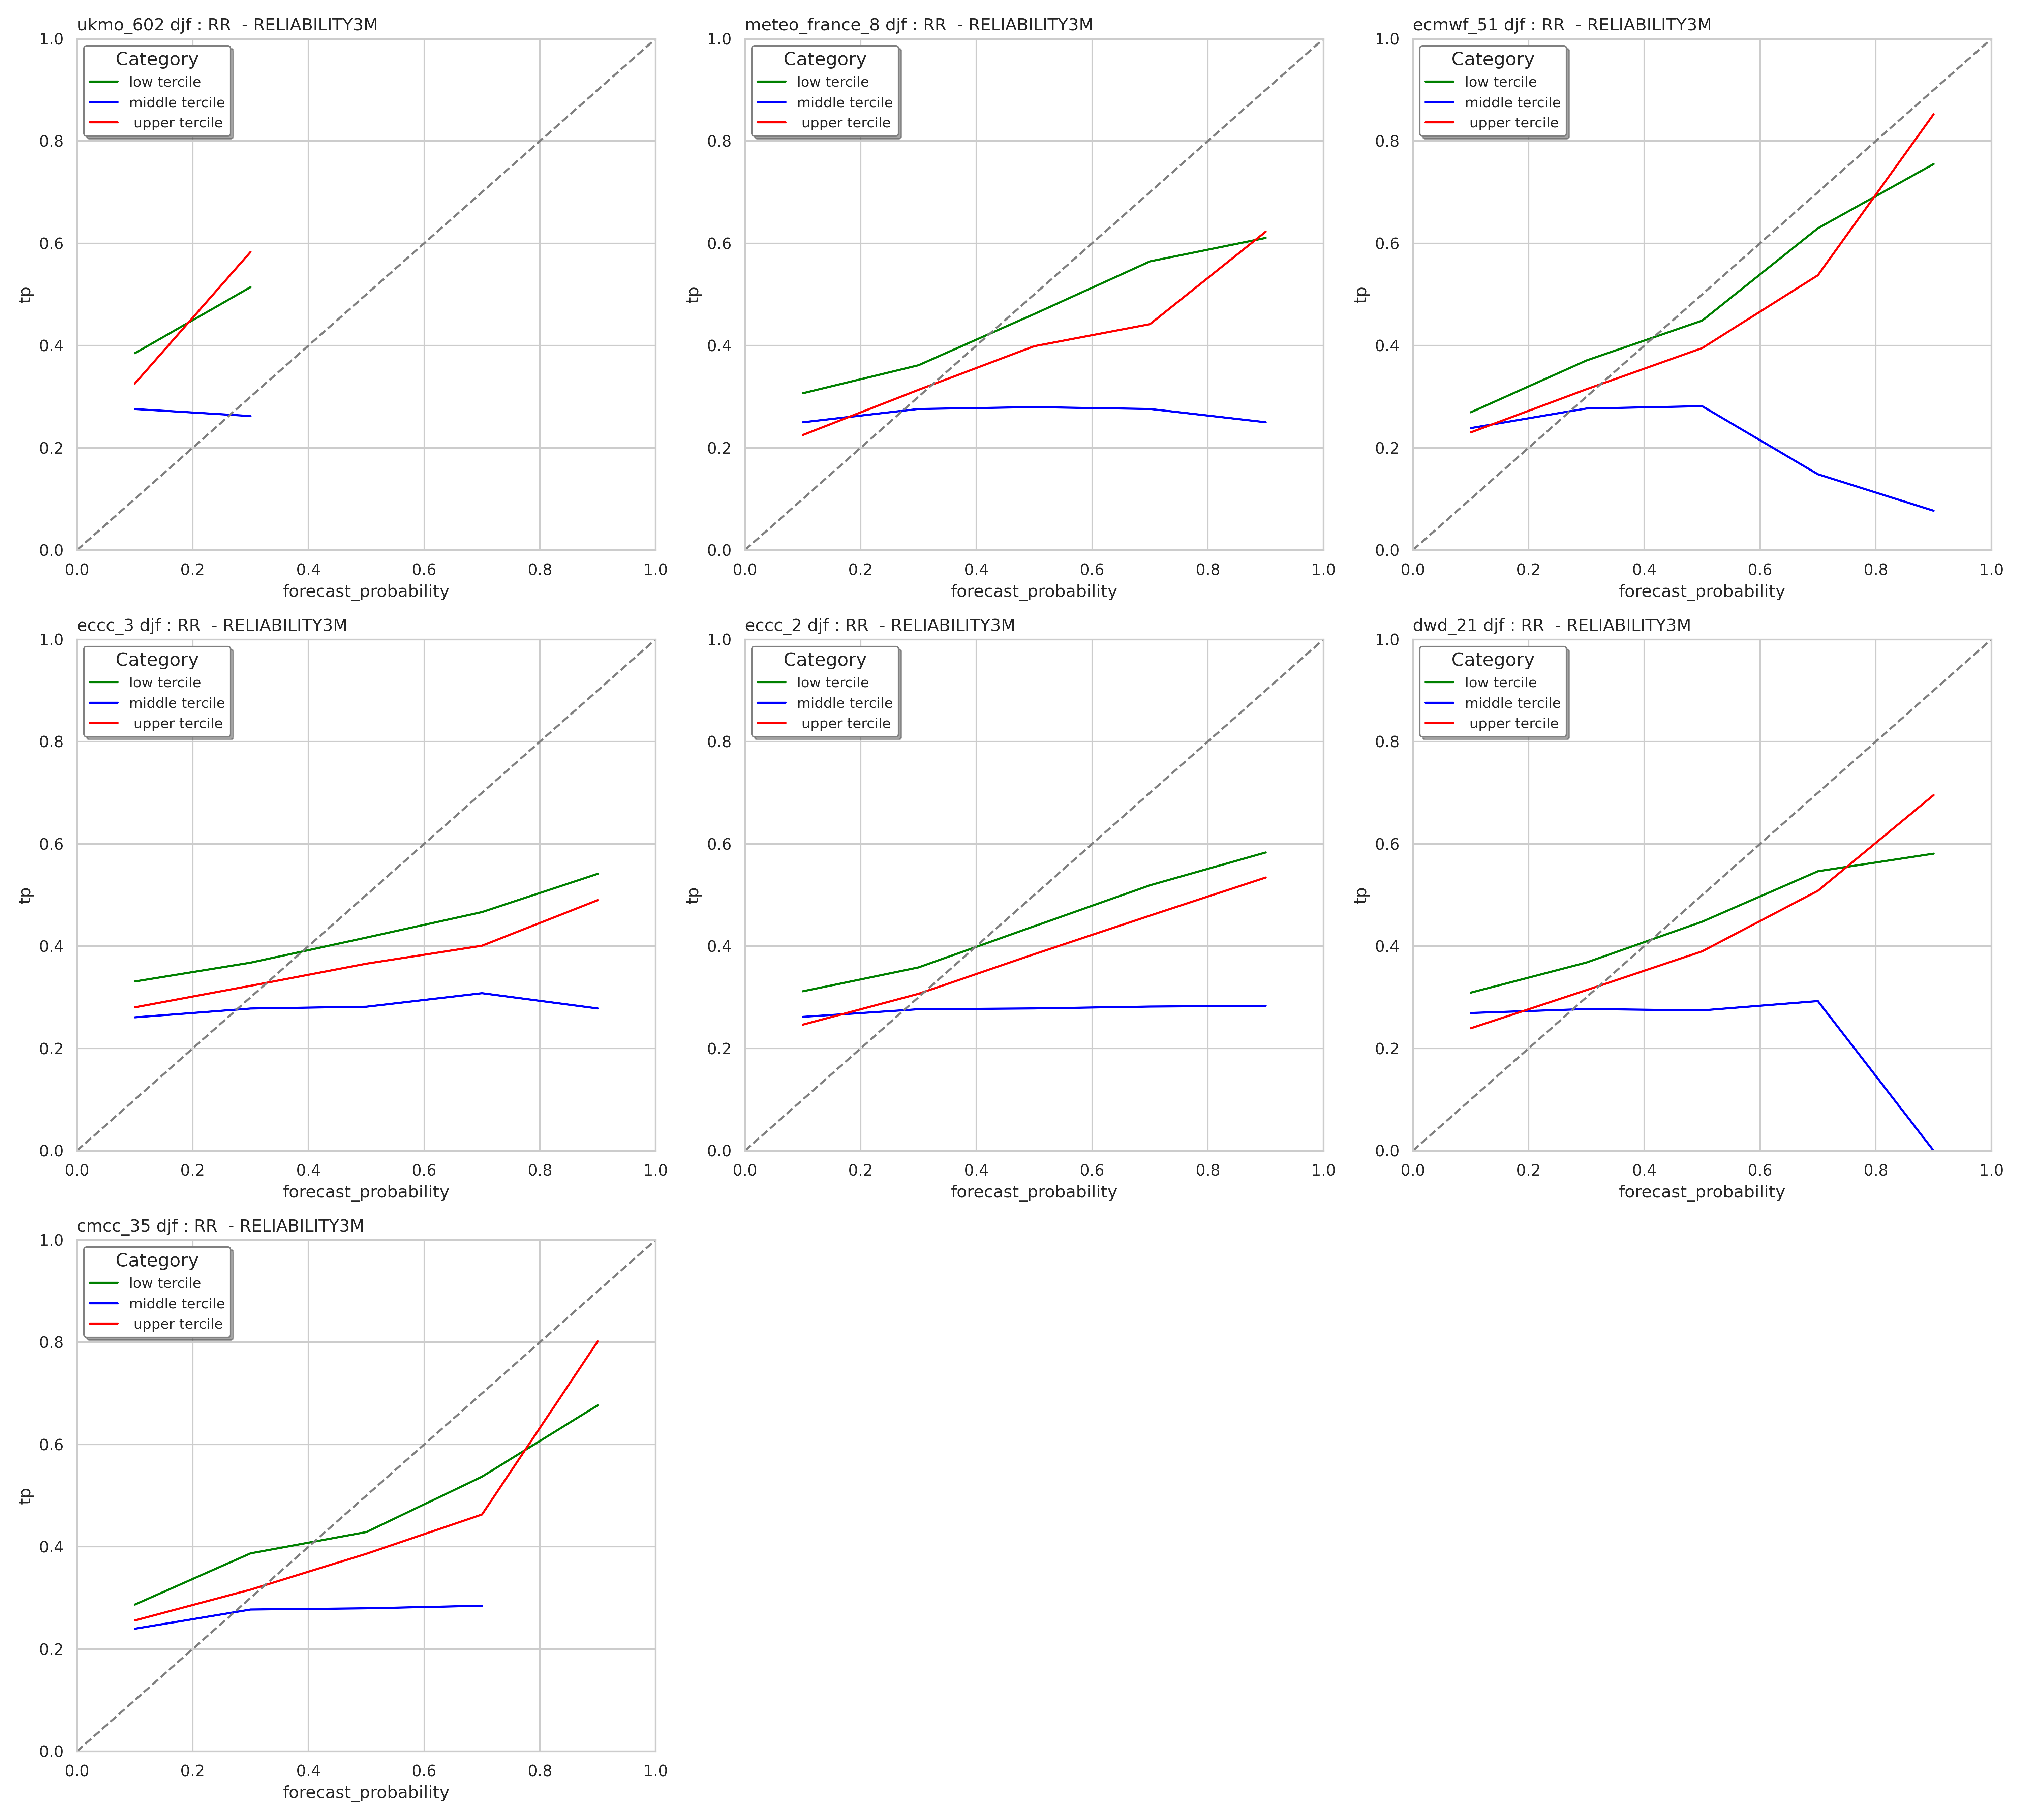
\includegraphics[scale=0.3]{plots/prob/rela/rela_diagram_RR_djf.png}
\caption{The 3-month rolling mean for Reliability DJF   . \textbf{\textit{Reliability is better in cases where the graphs are closer to the 45-degree line}}}
\end{figure}

for the reliability diagram, all centers show moderate results, except for the ukmo that shows lower reliability.Thus, for the lower and upper terciles, models in general show good reliability, but for the middle tercile, this models aren't reliable. above all, \textbf{\textit{ecmwf}}  shows the highest performance for reliability.


\subsubsection{The ranked probability score (RPS)}


\begin{figure}[H]
    \centering
    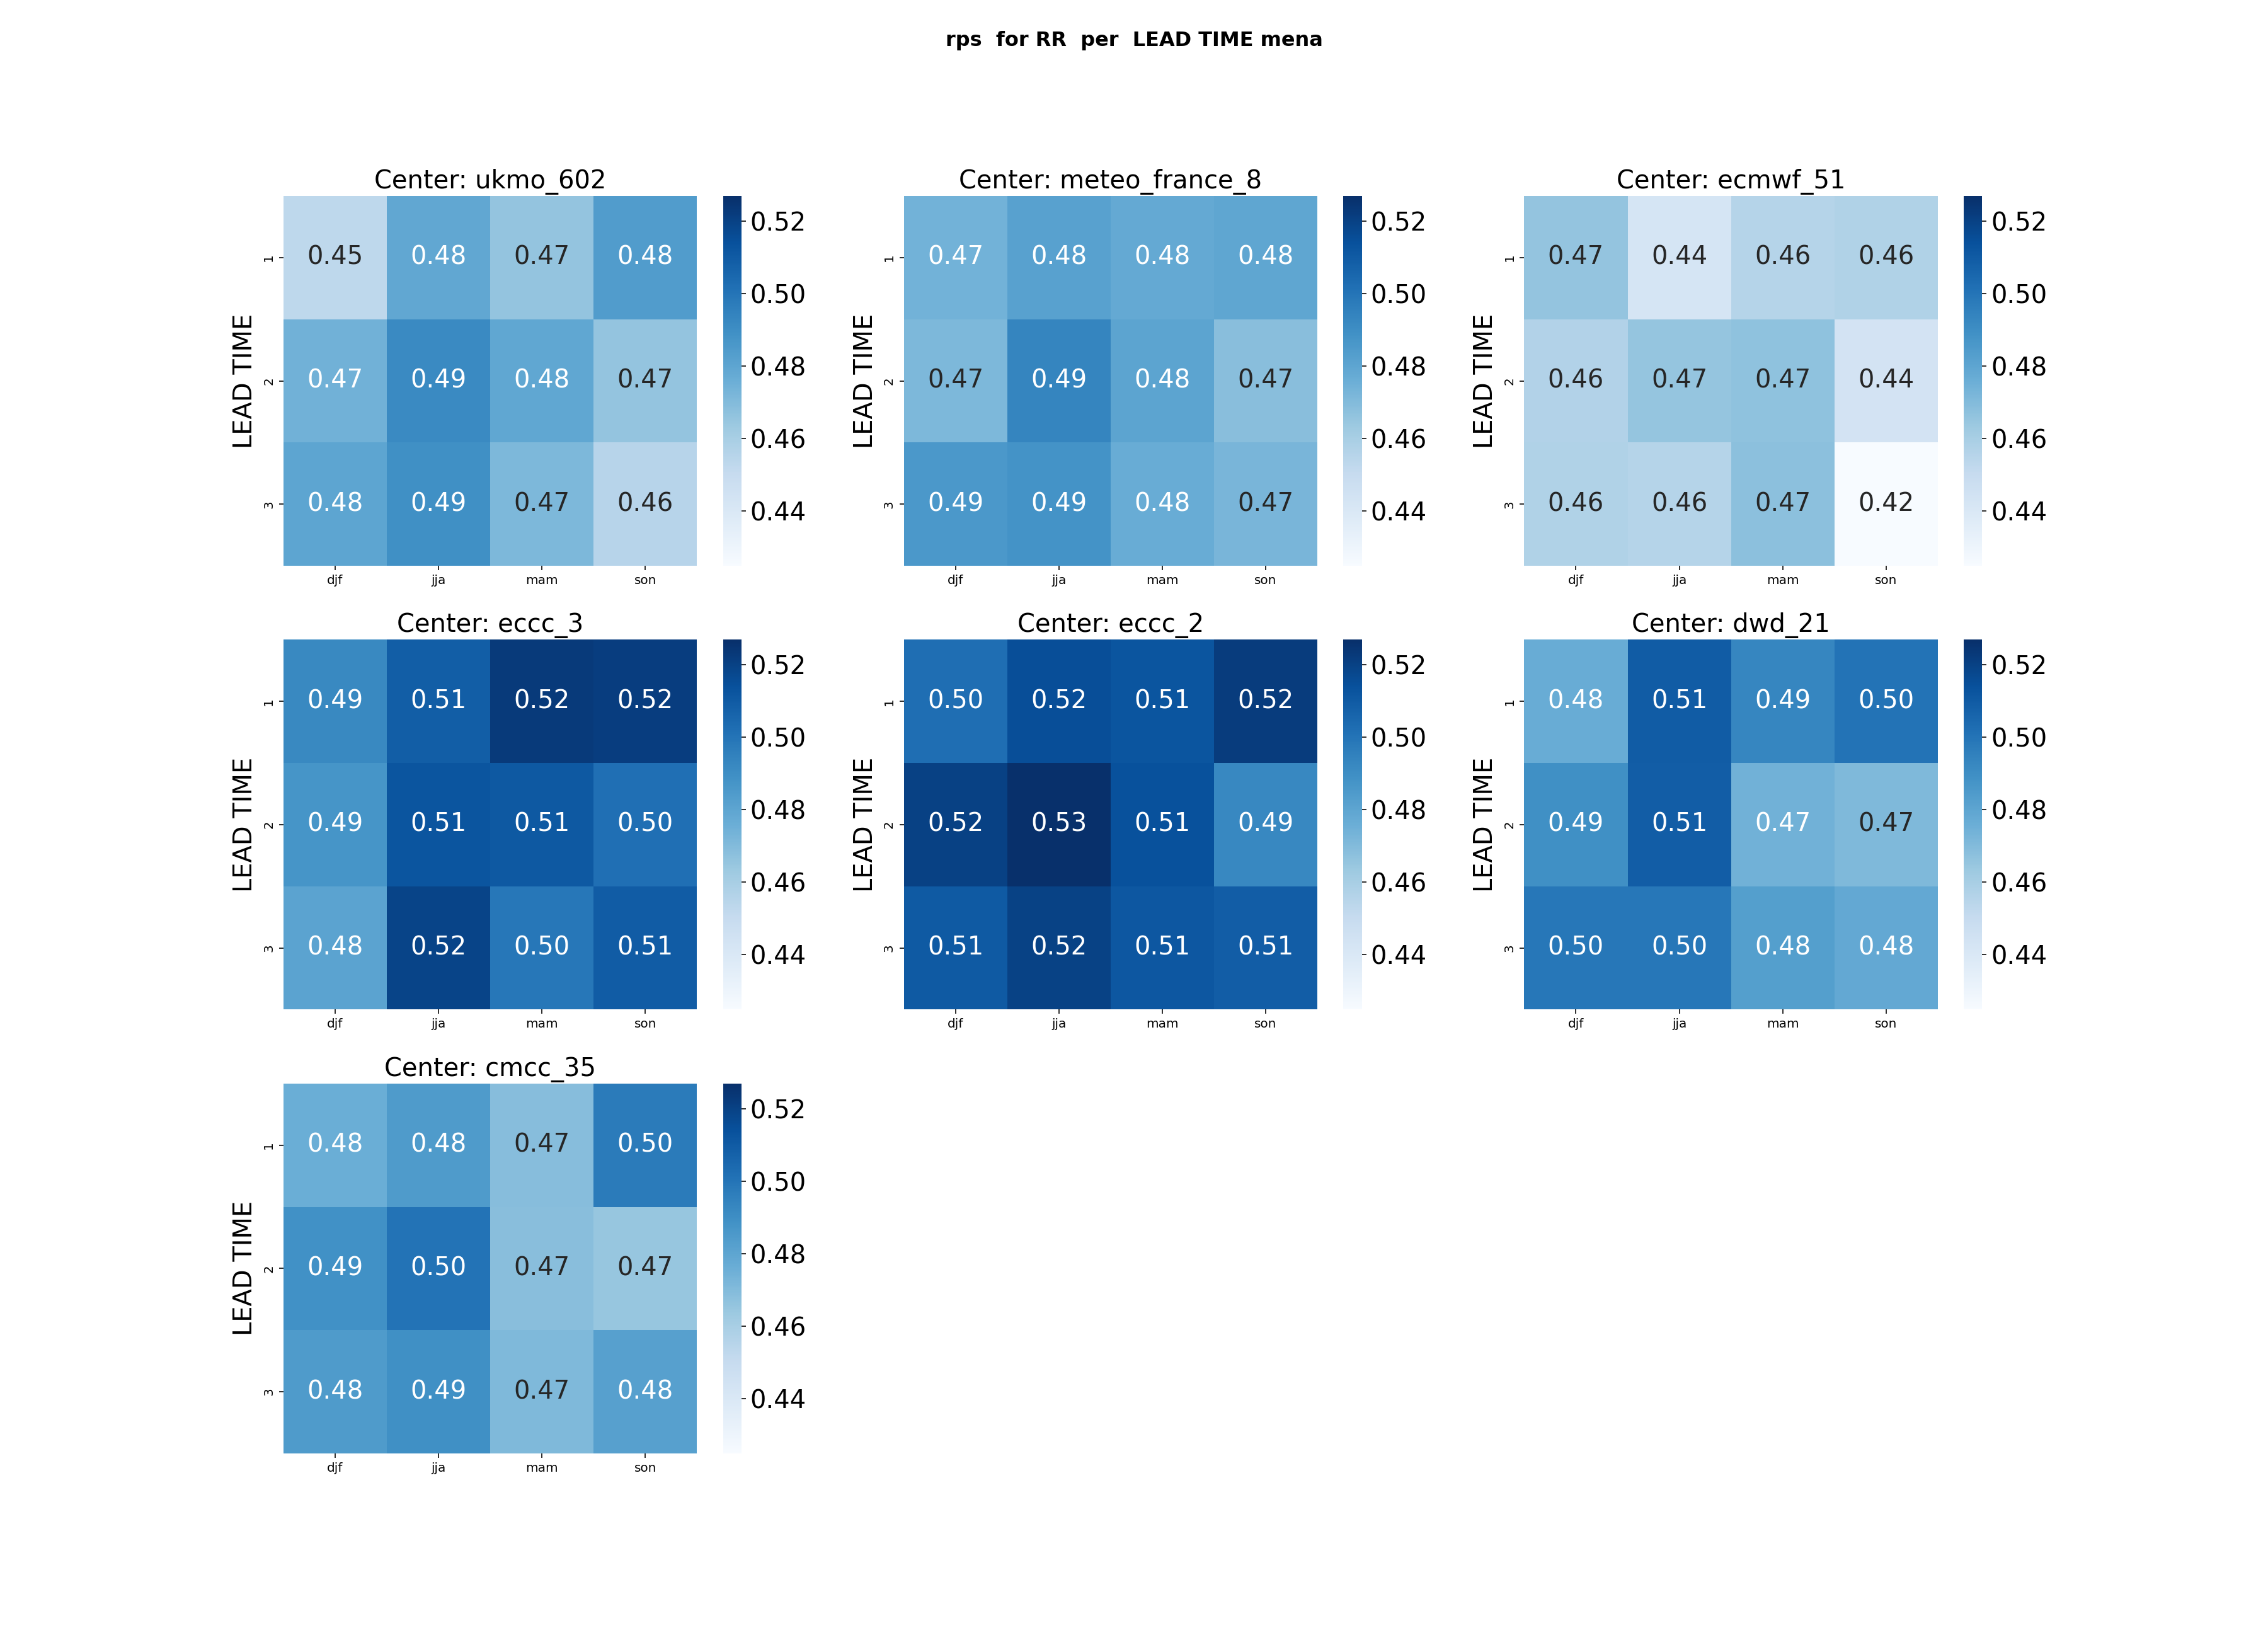
\includegraphics[scale=0.25]{plots/prob/rps/rps_RR_mena.png}
    \caption{The Heatmap of  RPS Score on MENA region for Precipitations    . \textbf{\textit{(0 means perfect RPS)}}}
\end{figure}

In the figure above, all centers demonstrate moderate performance, except for UKMO, which shows noticeably lower performance. 


\begin{figure}[H]
    \centering
    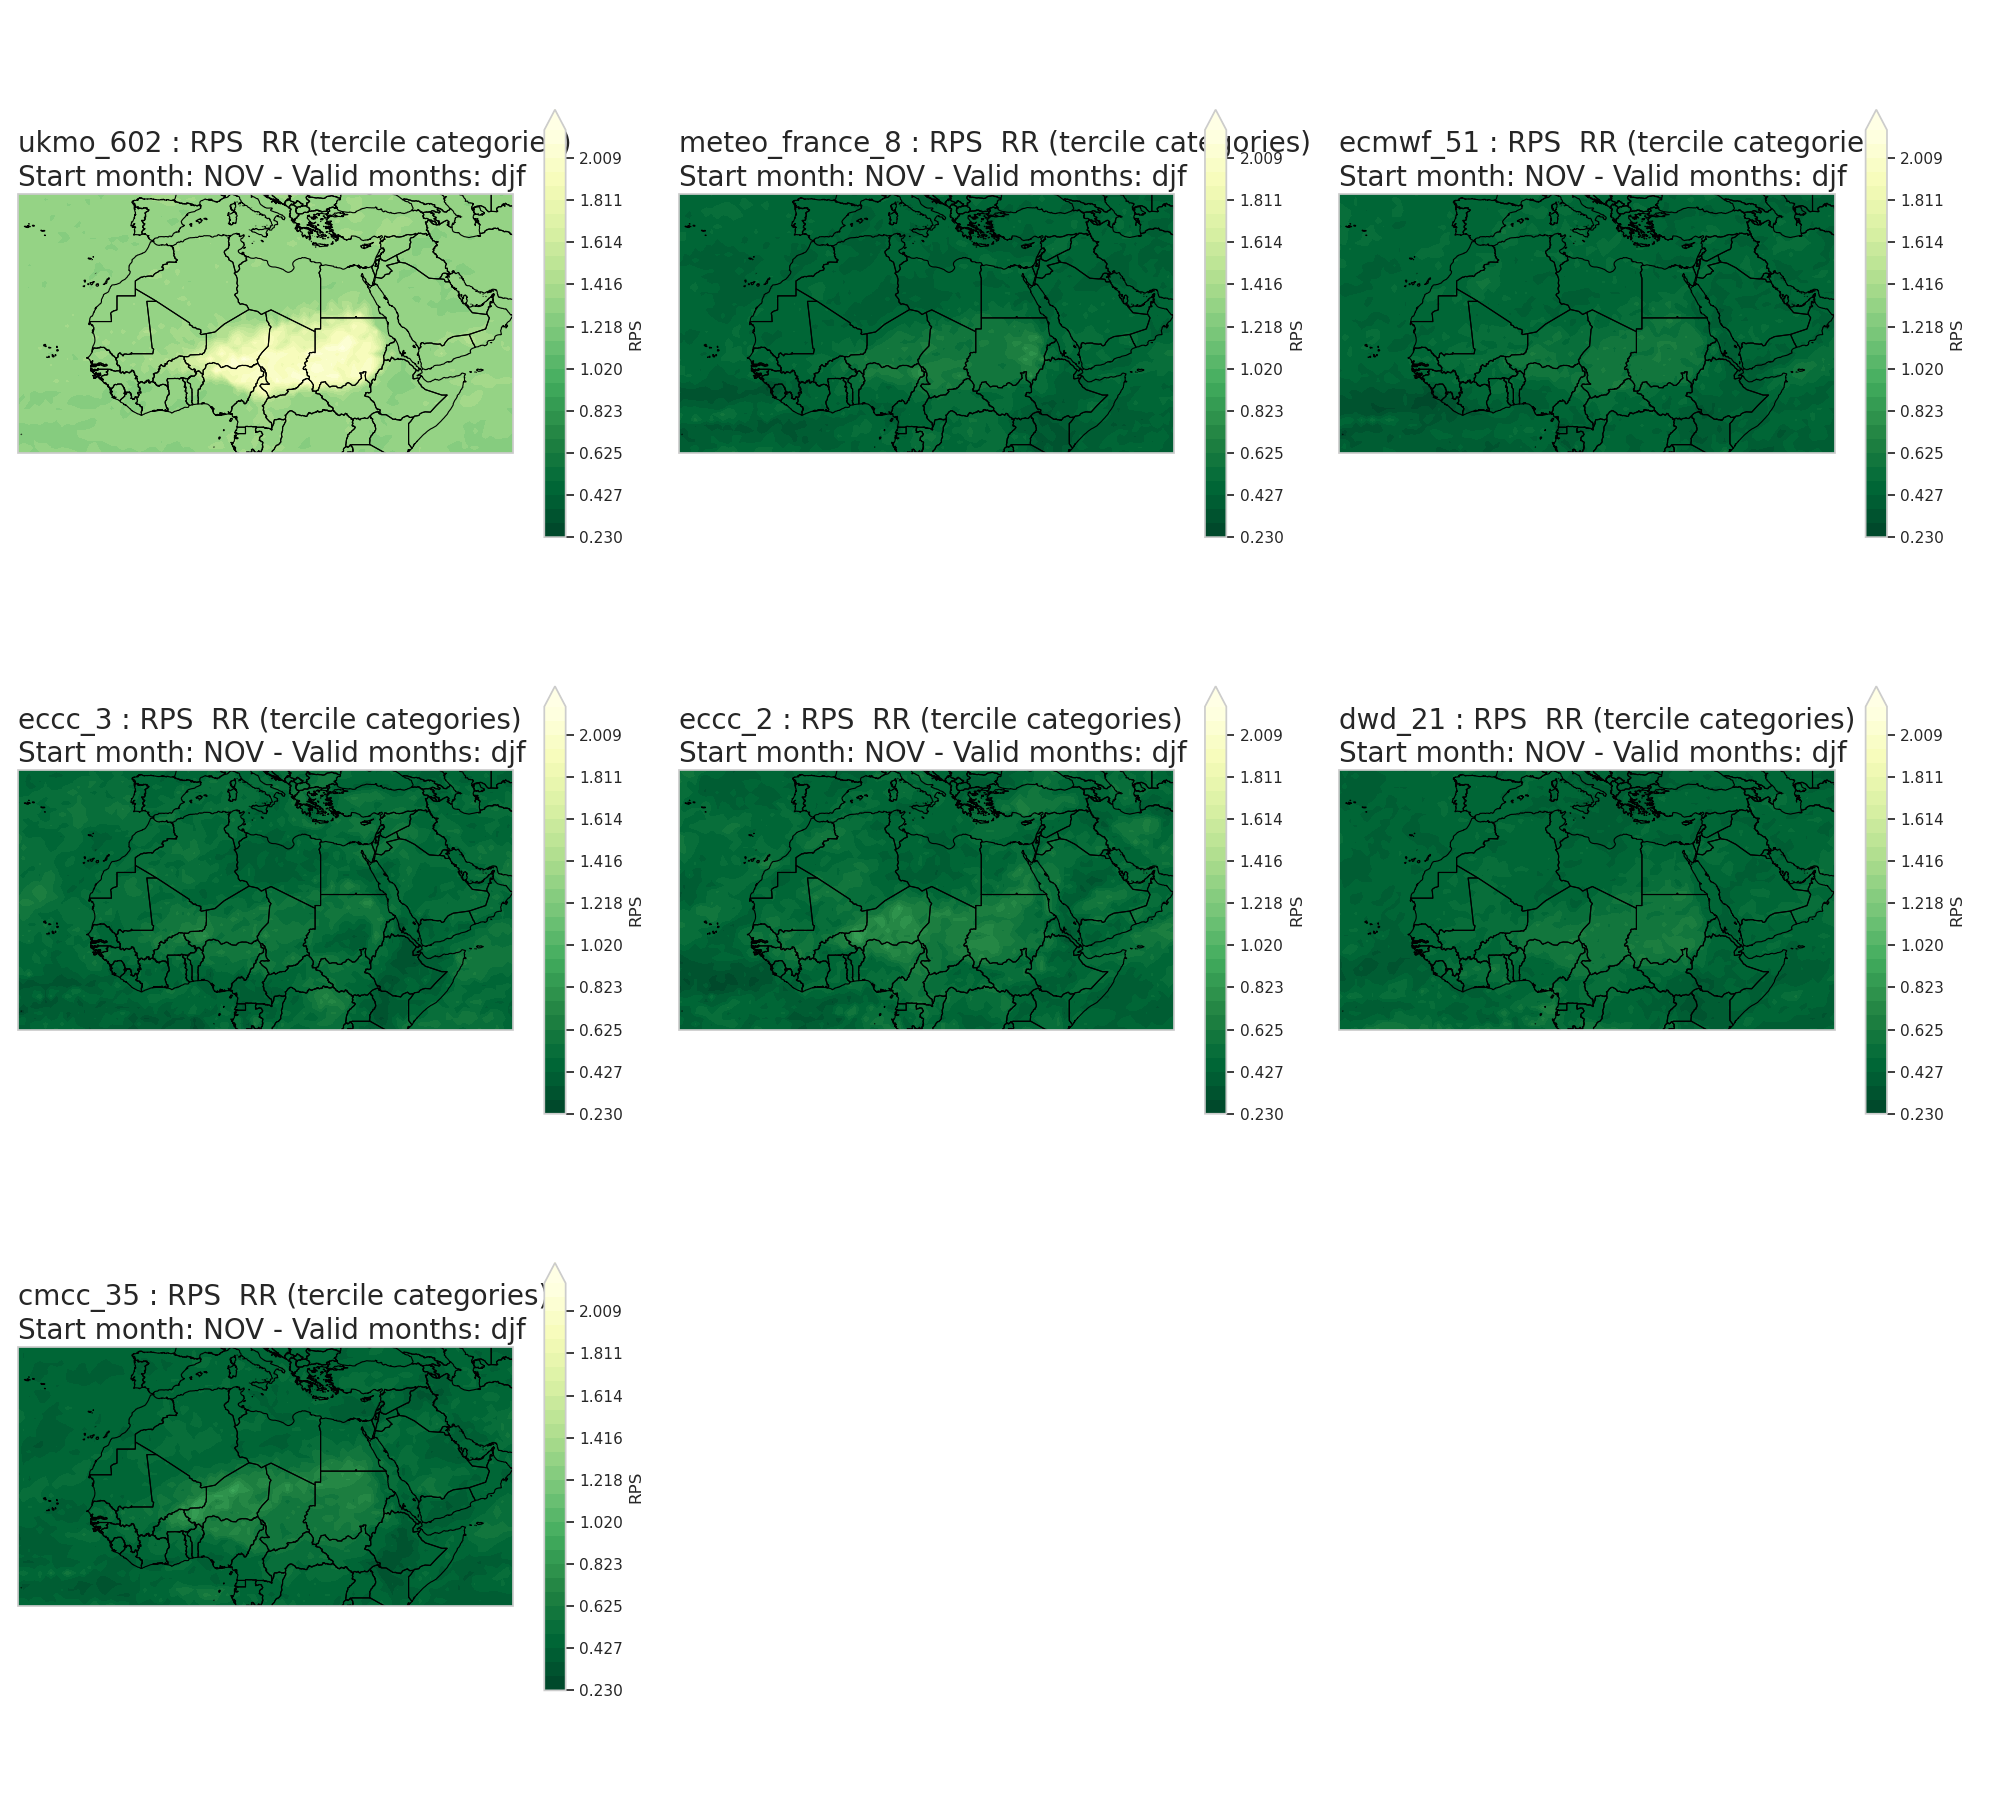
\includegraphics[scale=0.25]{plots/prob/rps/rps_djf_RR.png}
    \caption{The   RPS Score on MENA region for Precipitations DJF   . \textbf{\textit{(0 means perfect RPS)}}}
\end{figure}

the spacial distribution of the RPS, is homogeneous, in all the region the score is good for all centers.Thus, the ukmo shows lower performance for this score.




\subsubsection{Relative operating characteristics}

\begin{figure}[H]
    \centering
    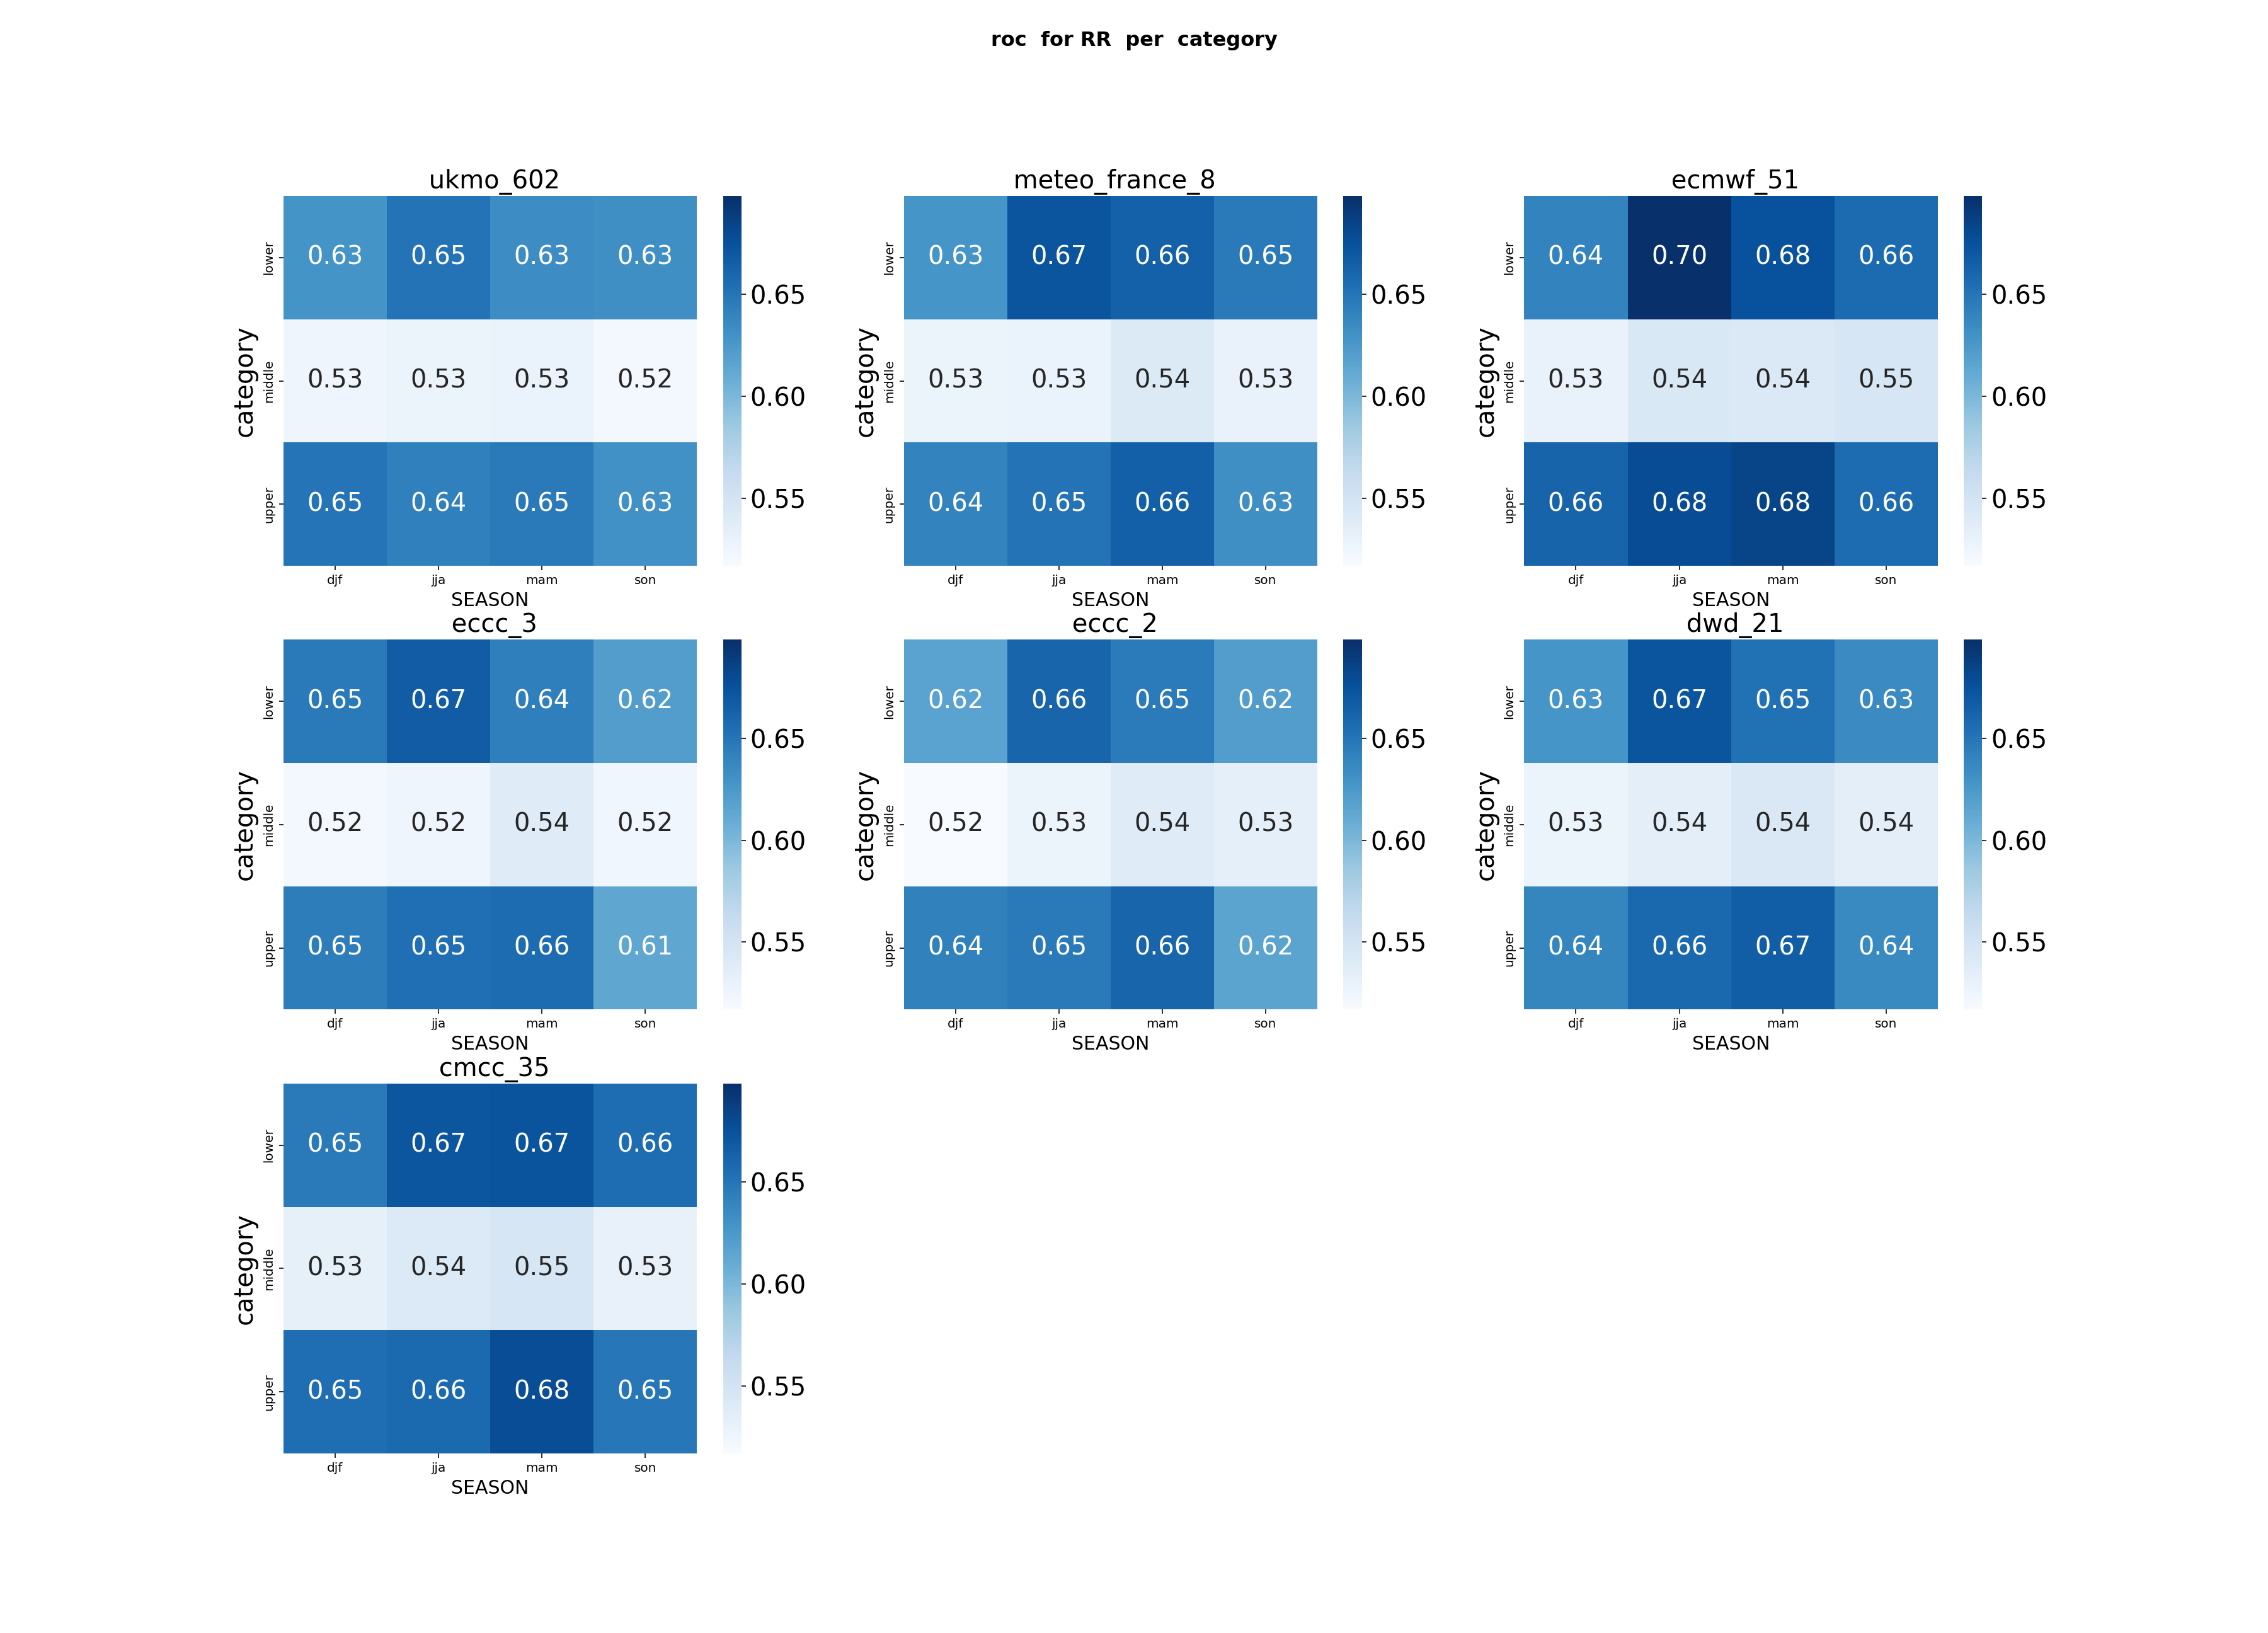
\includegraphics[scale=0.25]{plots/prob/roc/roc_RR_category.png}
    \caption{The Heatmap of ROC Score for each category  . \textbf{\textit{(1 means perfect ROC)}}}
\end{figure}

In the figure above, it is evident that all centers exhibit similar performance levels. However, the middle tercile consistently achieves the lowest score.
\begin{figure}[H]
    \centering
    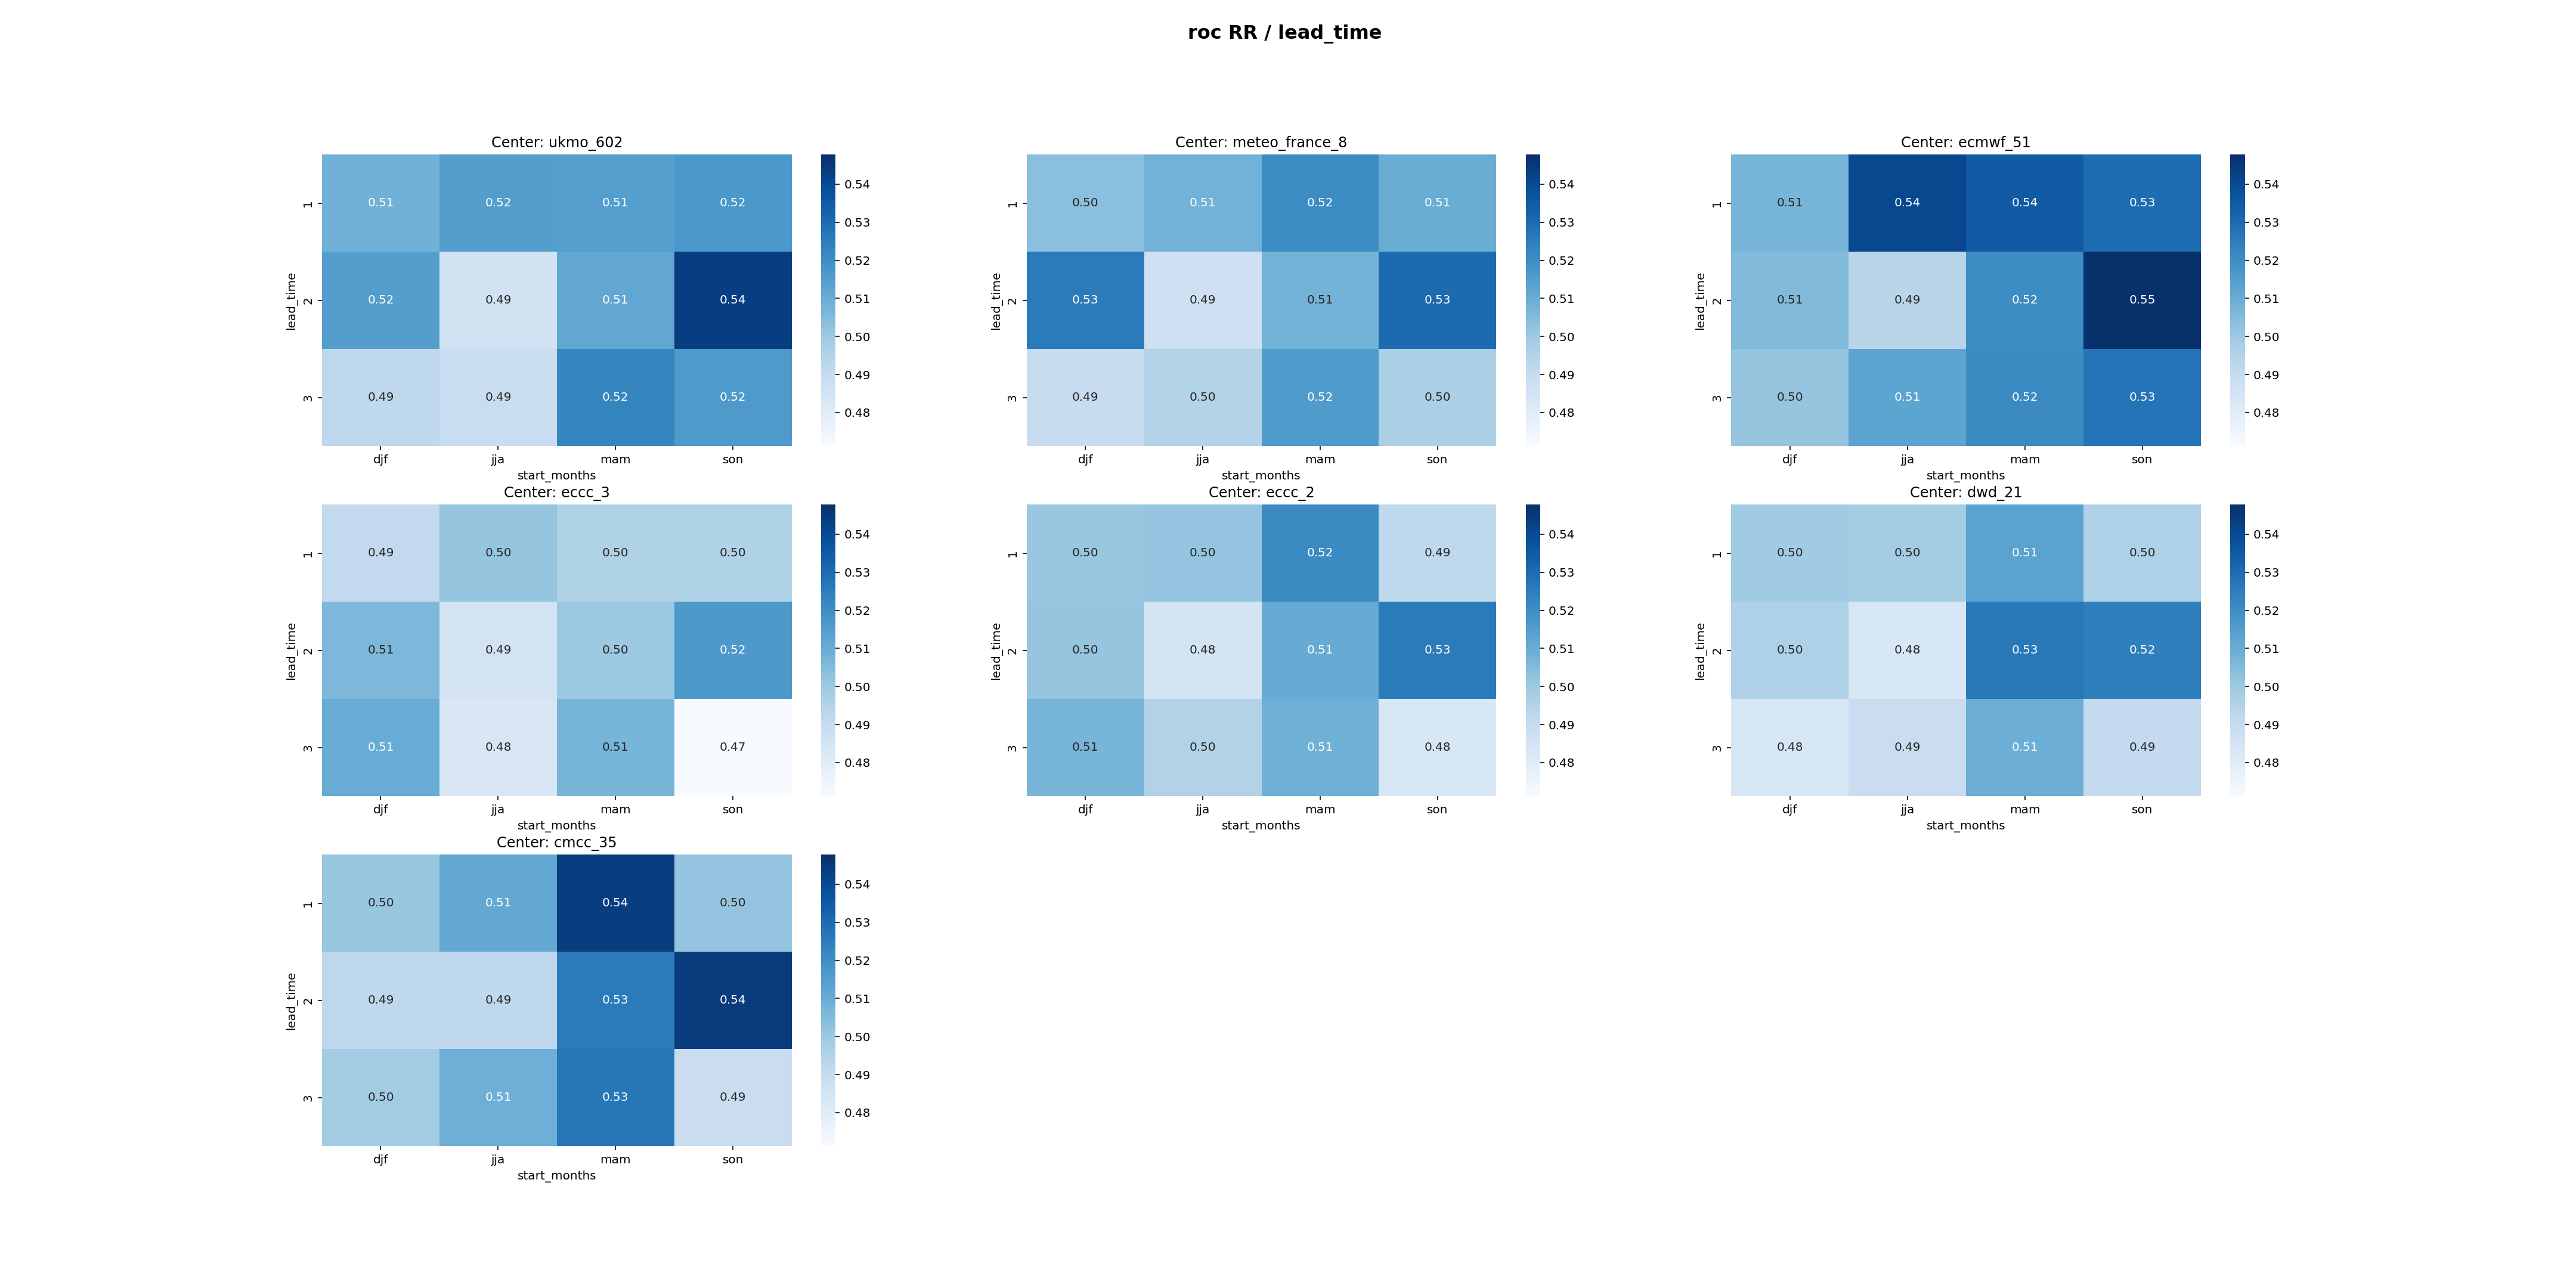
\includegraphics[scale=0.25]{plots/prob/roc/roc_RR_lead_time.png}
    \caption{The Heatmap of ROC Score for lead-times. \textbf{\textit{(1 means perfect ROC)}}}
\end{figure}

for the ROC score, all centers show similar good performance, in general the best score is observed for tha first lead-time, except for the SON season where the best performance is for the second lead-time.

\begin{figure}[H]
    \centering
    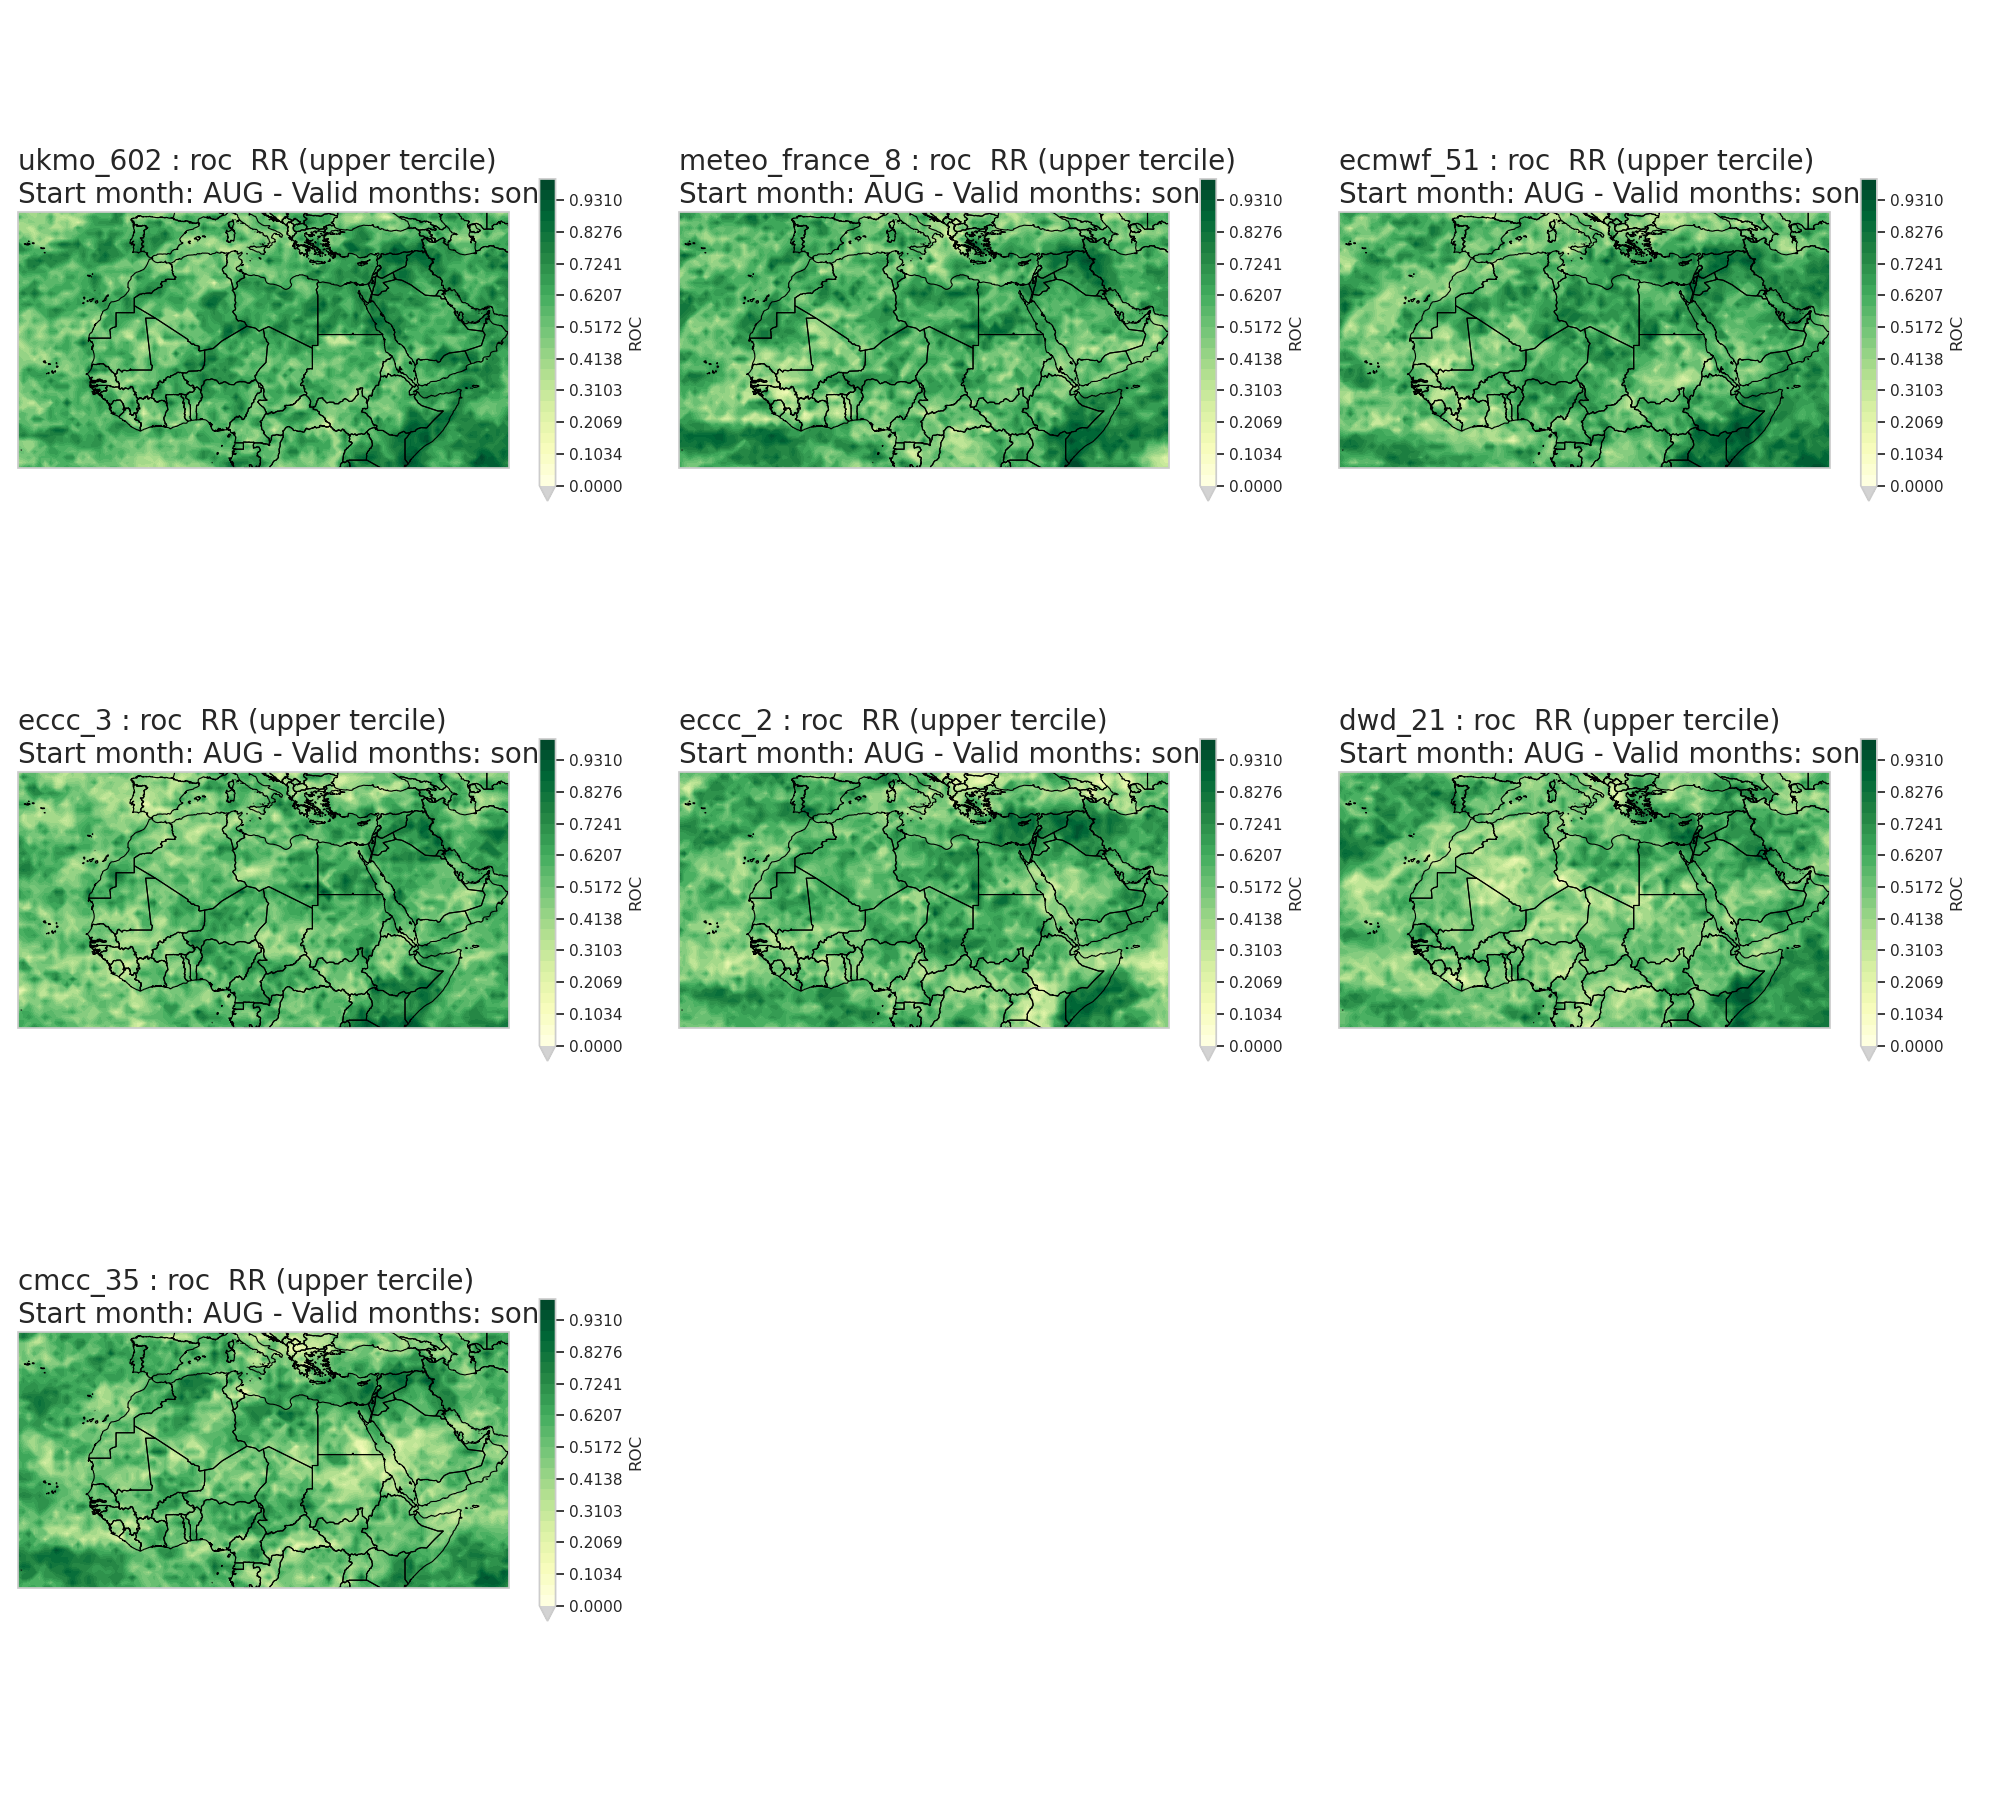
\includegraphics[scale=0.3]{plots/prob/roc/roc_son_RR_upper.png}
    \caption{The ROC Score Upper tercile SON    . \textbf{\textit{(1 means perfect ROC)}}}
\end{figure}

the spacial distribution of the roc score confirms an important result. For precipitation all centers shows better performance for the East of Africa, Irak,Syria,Jordan and Palestine. The performance in this zone is very high (score near to 1). For the rest of MENA region the performance is similar, with moderate to good score.

																
\subsubsection{Relative operating characteristics Skill Score}

In the figure above, the ECMWF exhibit the best performance for all terciles and periods. However, we should notice that the performance is very low for the middle tercile in all centers. For the analysis along time, the performance is so low, the best performance is in the first lead-time, except the SON which shows the best performance for the second lead-time. Above all, the \textbf{\textit{ecmwf}} shows the best performance.

\begin{figure}[H]
    \centering
    \includegraphics[scale=0.25]{plots/prob/rocss/rocss_RR_category.png}
    \caption{The ROCSS Score for each category  . \textbf{\textit{(1 means perfect ROCSS)}}}
\end{figure}


\begin{figure}[H]
    \centering
    \includegraphics[scale=0.25]{plots/prob/rocss/rocss_RR_lead_time.png}
    \caption{The average of  ROCSS Score on all categories    . \textbf{\textit{(1 means perfect ROCSS)}}}
\end{figure}



\begin{figure}[H]
    \centering
    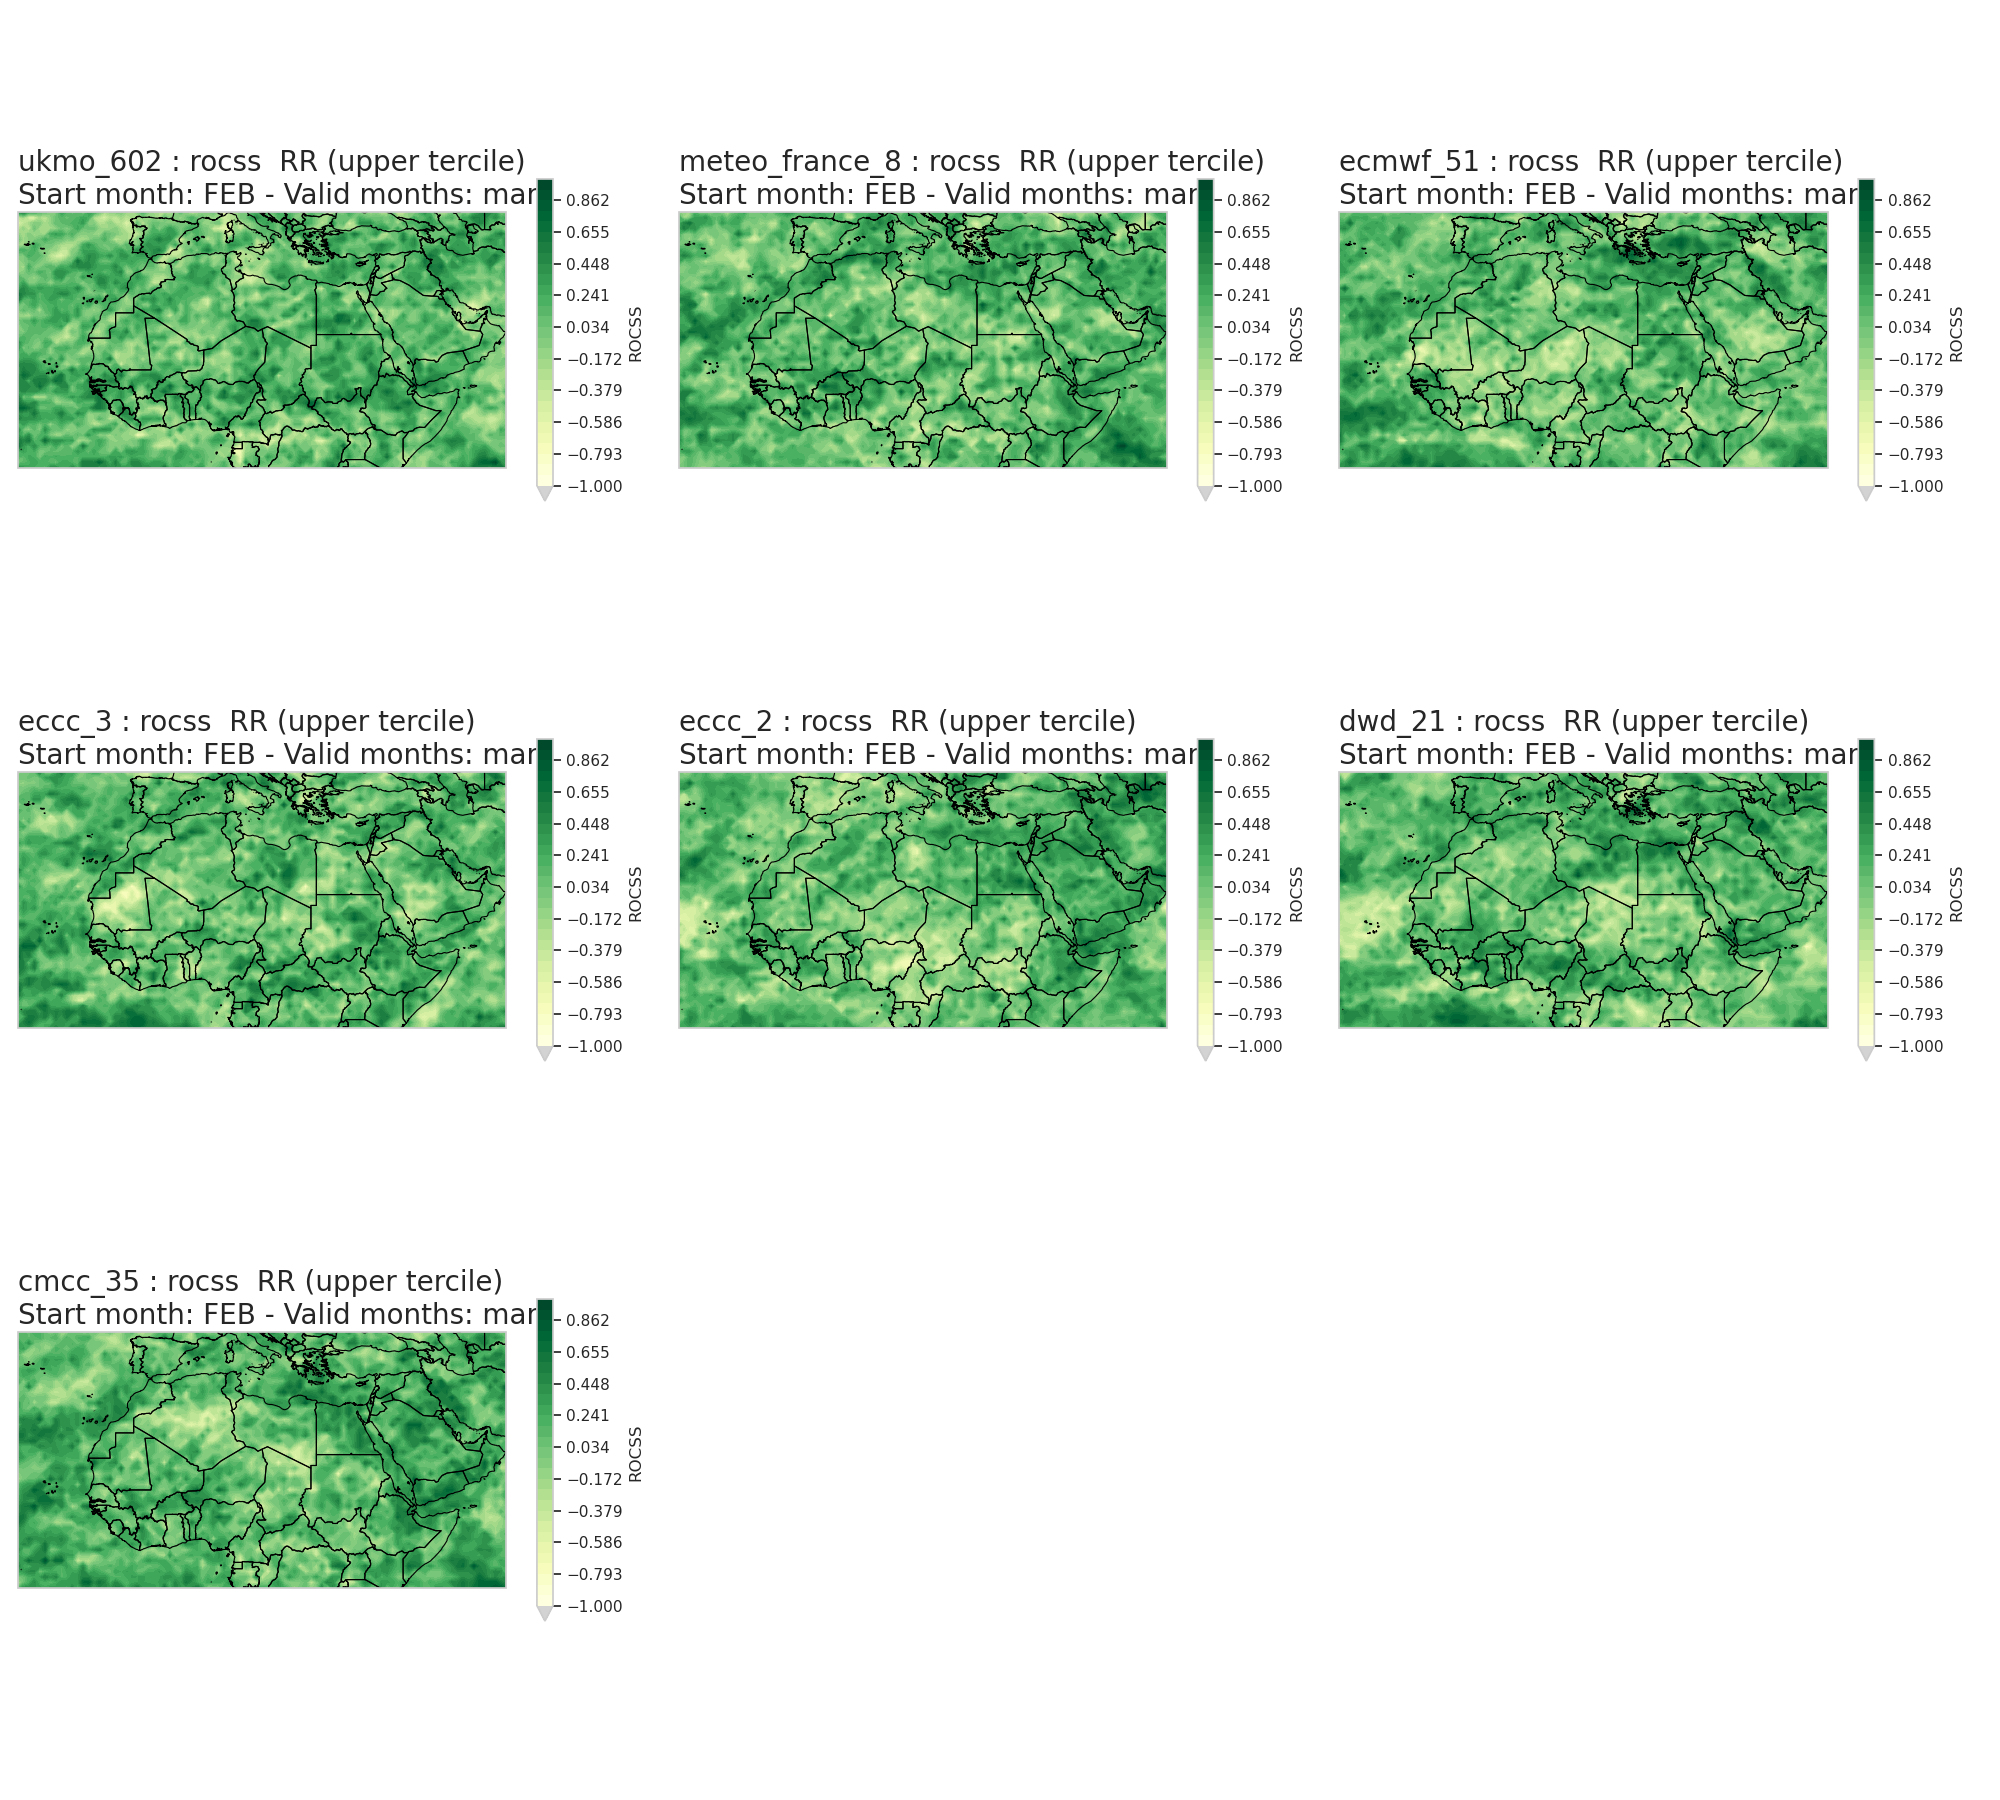
\includegraphics[scale=0.3]{plots/prob/rocss/rocss_mam_RR_upper.png}
    \caption{The ROC Skill Score Upper tercile MAM    . \textbf{\textit{(1 means perfect ROCSS)}}}
\end{figure}

the spacial distribution of the ROCSS, shows that all centers are consistent for this score. The spacial distribution isn't clear, there is a high spacial variability.



\subsubsection{summary}
\begin{table}[h!]
\centering
\begin{tabularx}{\textwidth}{@{}p{2.5cm}p{4cm}p{4cm}p{2.5cm}p{3cm}@{}}
\toprule
\textbf{Metric}       & \textbf{Focus}                                    & \textbf{What it Measures}                         & \textbf{Dependent on Observed Outcomes?} & \textbf{Visualization/Tools}             \\ \midrule
\textbf{Reliability}   & Probabilities match observed frequencies          & Calibration of probabilities                      & Yes                                      & Reliability diagram                      \\
\textbf{Discrimination} & Differentiating between outcomes                 & Ability to distinguish events from non-events    & Yes                                      & ROC curve, AUC                           \\
\textbf{Sharpness}     & Boldness of probabilities (away from average)     & Confidence of the forecast                        & No                                       & Histogram of forecast probabilities      \\
\textbf{Resolution}    & Informativeness and variability of forecast       & Ability to provide specific, useful info         & Yes                                      & Brier Score decomposition                \\ \bottomrule
\end{tabularx}
\caption{Key differences between reliability, discrimination, sharpness, and resolution in seasonal forecasting.}
\label{tab:forecast_metrics}
\end{table}

\newpage
\thispagestyle{empty}
\mbox{}

\endinput 


\chapter{Regional Performance Evaluation: North Africa and Arabian Peninsula}
\section{temperature}
\subsection{Deterministic Evaluation Metrics}

\subsubsection{Analysis of ACC Results}

\paragraph{Focus on North Africa}  
The heatmap below reveals that the \textbf{\textit{ECMWF}}, \textbf{\textit{UKMO}}, and \textbf{\textit{ECC\_3}} models demonstrate relatively strong correlations over the North Africa region. This suggests that these models perform well in capturing the anomalies in this specific area.  

\begin{figure}[H]
\centering
\includegraphics[scale=0.25]{plots/det/acc/acc_T2M_NorthAfrica.png}
\caption{ACC heatmap for the North Africa region across different periods.}
\end{figure}

\paragraph{Focus on the Arabian Peninsula}  
The heatmap for the Arabian Peninsula indicates strong performance across all forecasting centers, with \textbf{\textit{ECMWF}}, \textbf{\textit{UKMO}}, and \textbf{\textit{DWD}} exhibiting the highest correlation scores.  

\begin{figure}[H]
\centering
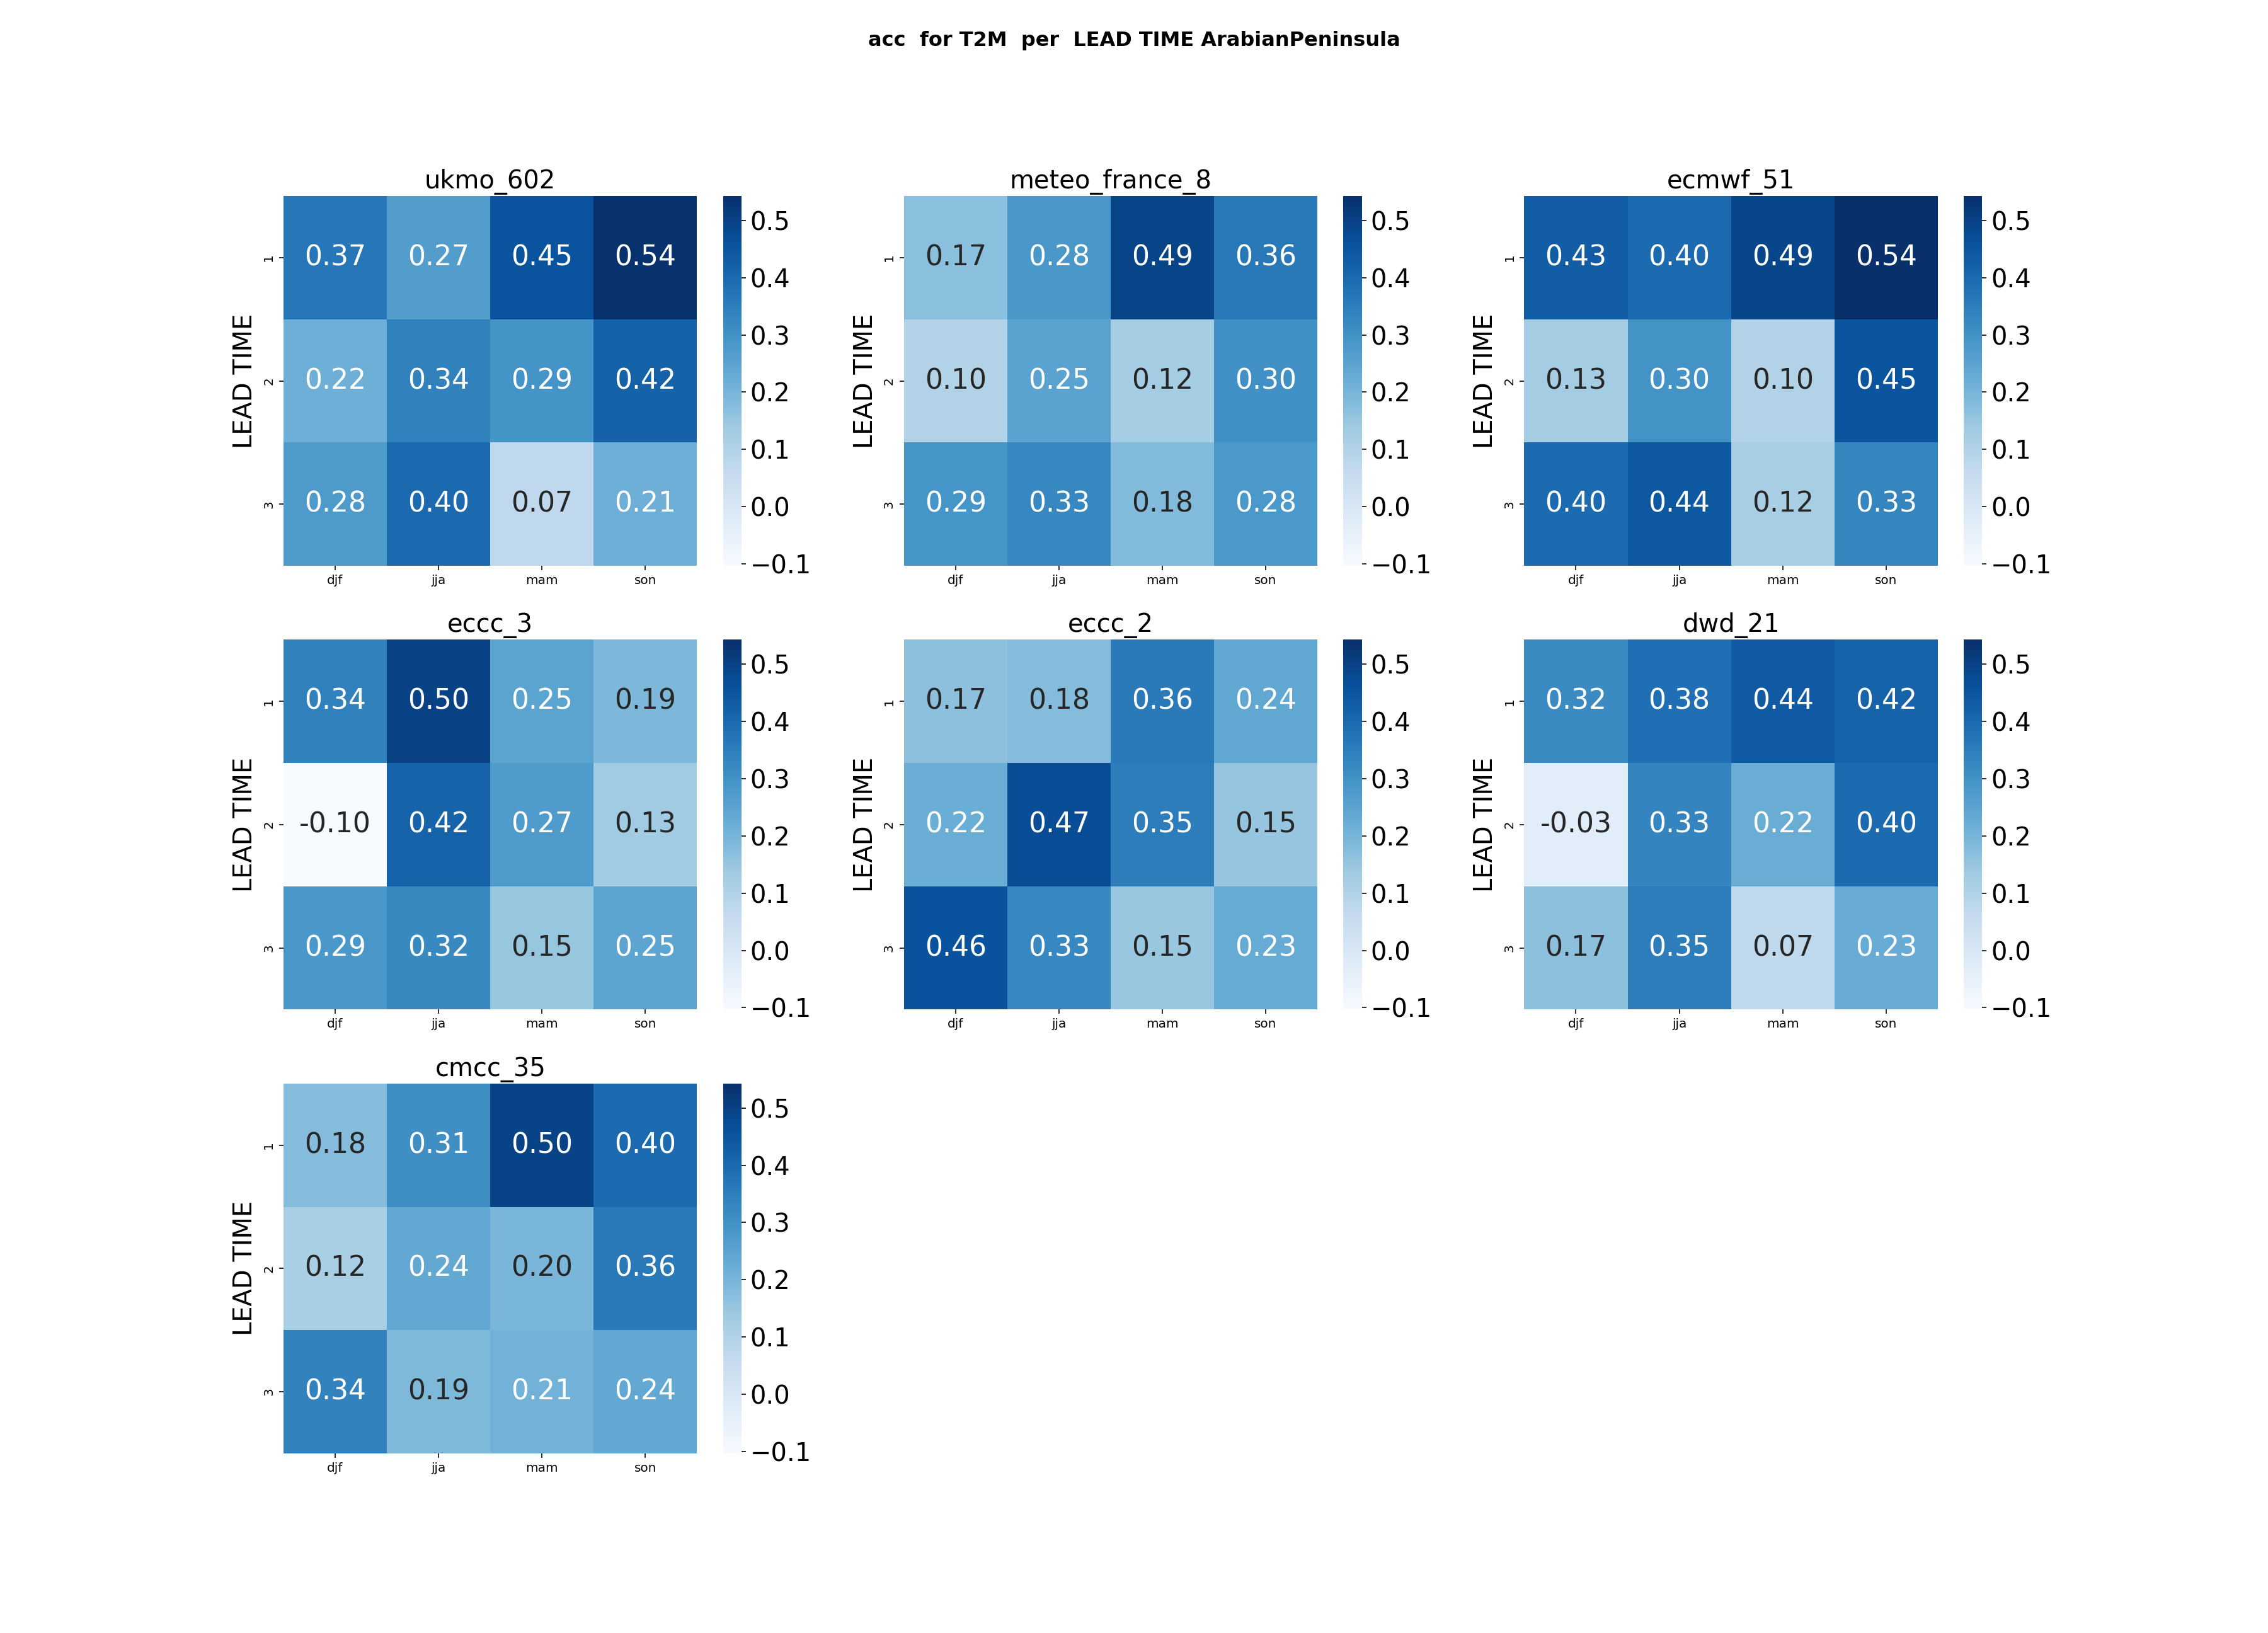
\includegraphics[scale=0.25]{plots/det/acc/acc_T2M_ArabianPeninsula.png}
\caption{ACC heatmap for the Arabian Peninsula across different periods \textbf{\textit{(1 indicates perfect correlation)}}.}
\end{figure}

The analysis highlights that the Arabian Peninsula consistently achieves better ACC scores compared to the general MENA region. Notably, the ACC is particularly high for \textbf{\textit{SON (September-October-November)}} at the third lead time.
\subsubsection{Analysis of RMSE Results}

\vspace{1.5cm}

\paragraph{focus on North Africa} : 
\begin{figure}[H]
\centering
\includegraphics[scale=0.3]{plots/det/rmse/rmse_T2M_NorthAfrica.png}
\caption{heatmap of RMSE For T2M  (North Africa)}
\end{figure}

The North African climate poses challenges for modeling extreme temperatures and spatial variability. Heatmap analysis shows that \textbf{\textit{ECMWF}} excels in JJA with RMSE values of 1.34°C–1.58°C but performs lower in other seasons. \textbf{\textit{Météo-France}} delivers consistent accuracy, especially in SON, making it more reliable for multi-seasonal forecasting in this region.
\vspace{1.5cm}
\paragraph{focus on Arabian Peninsula}:

\begin{figure}[H]
\centering
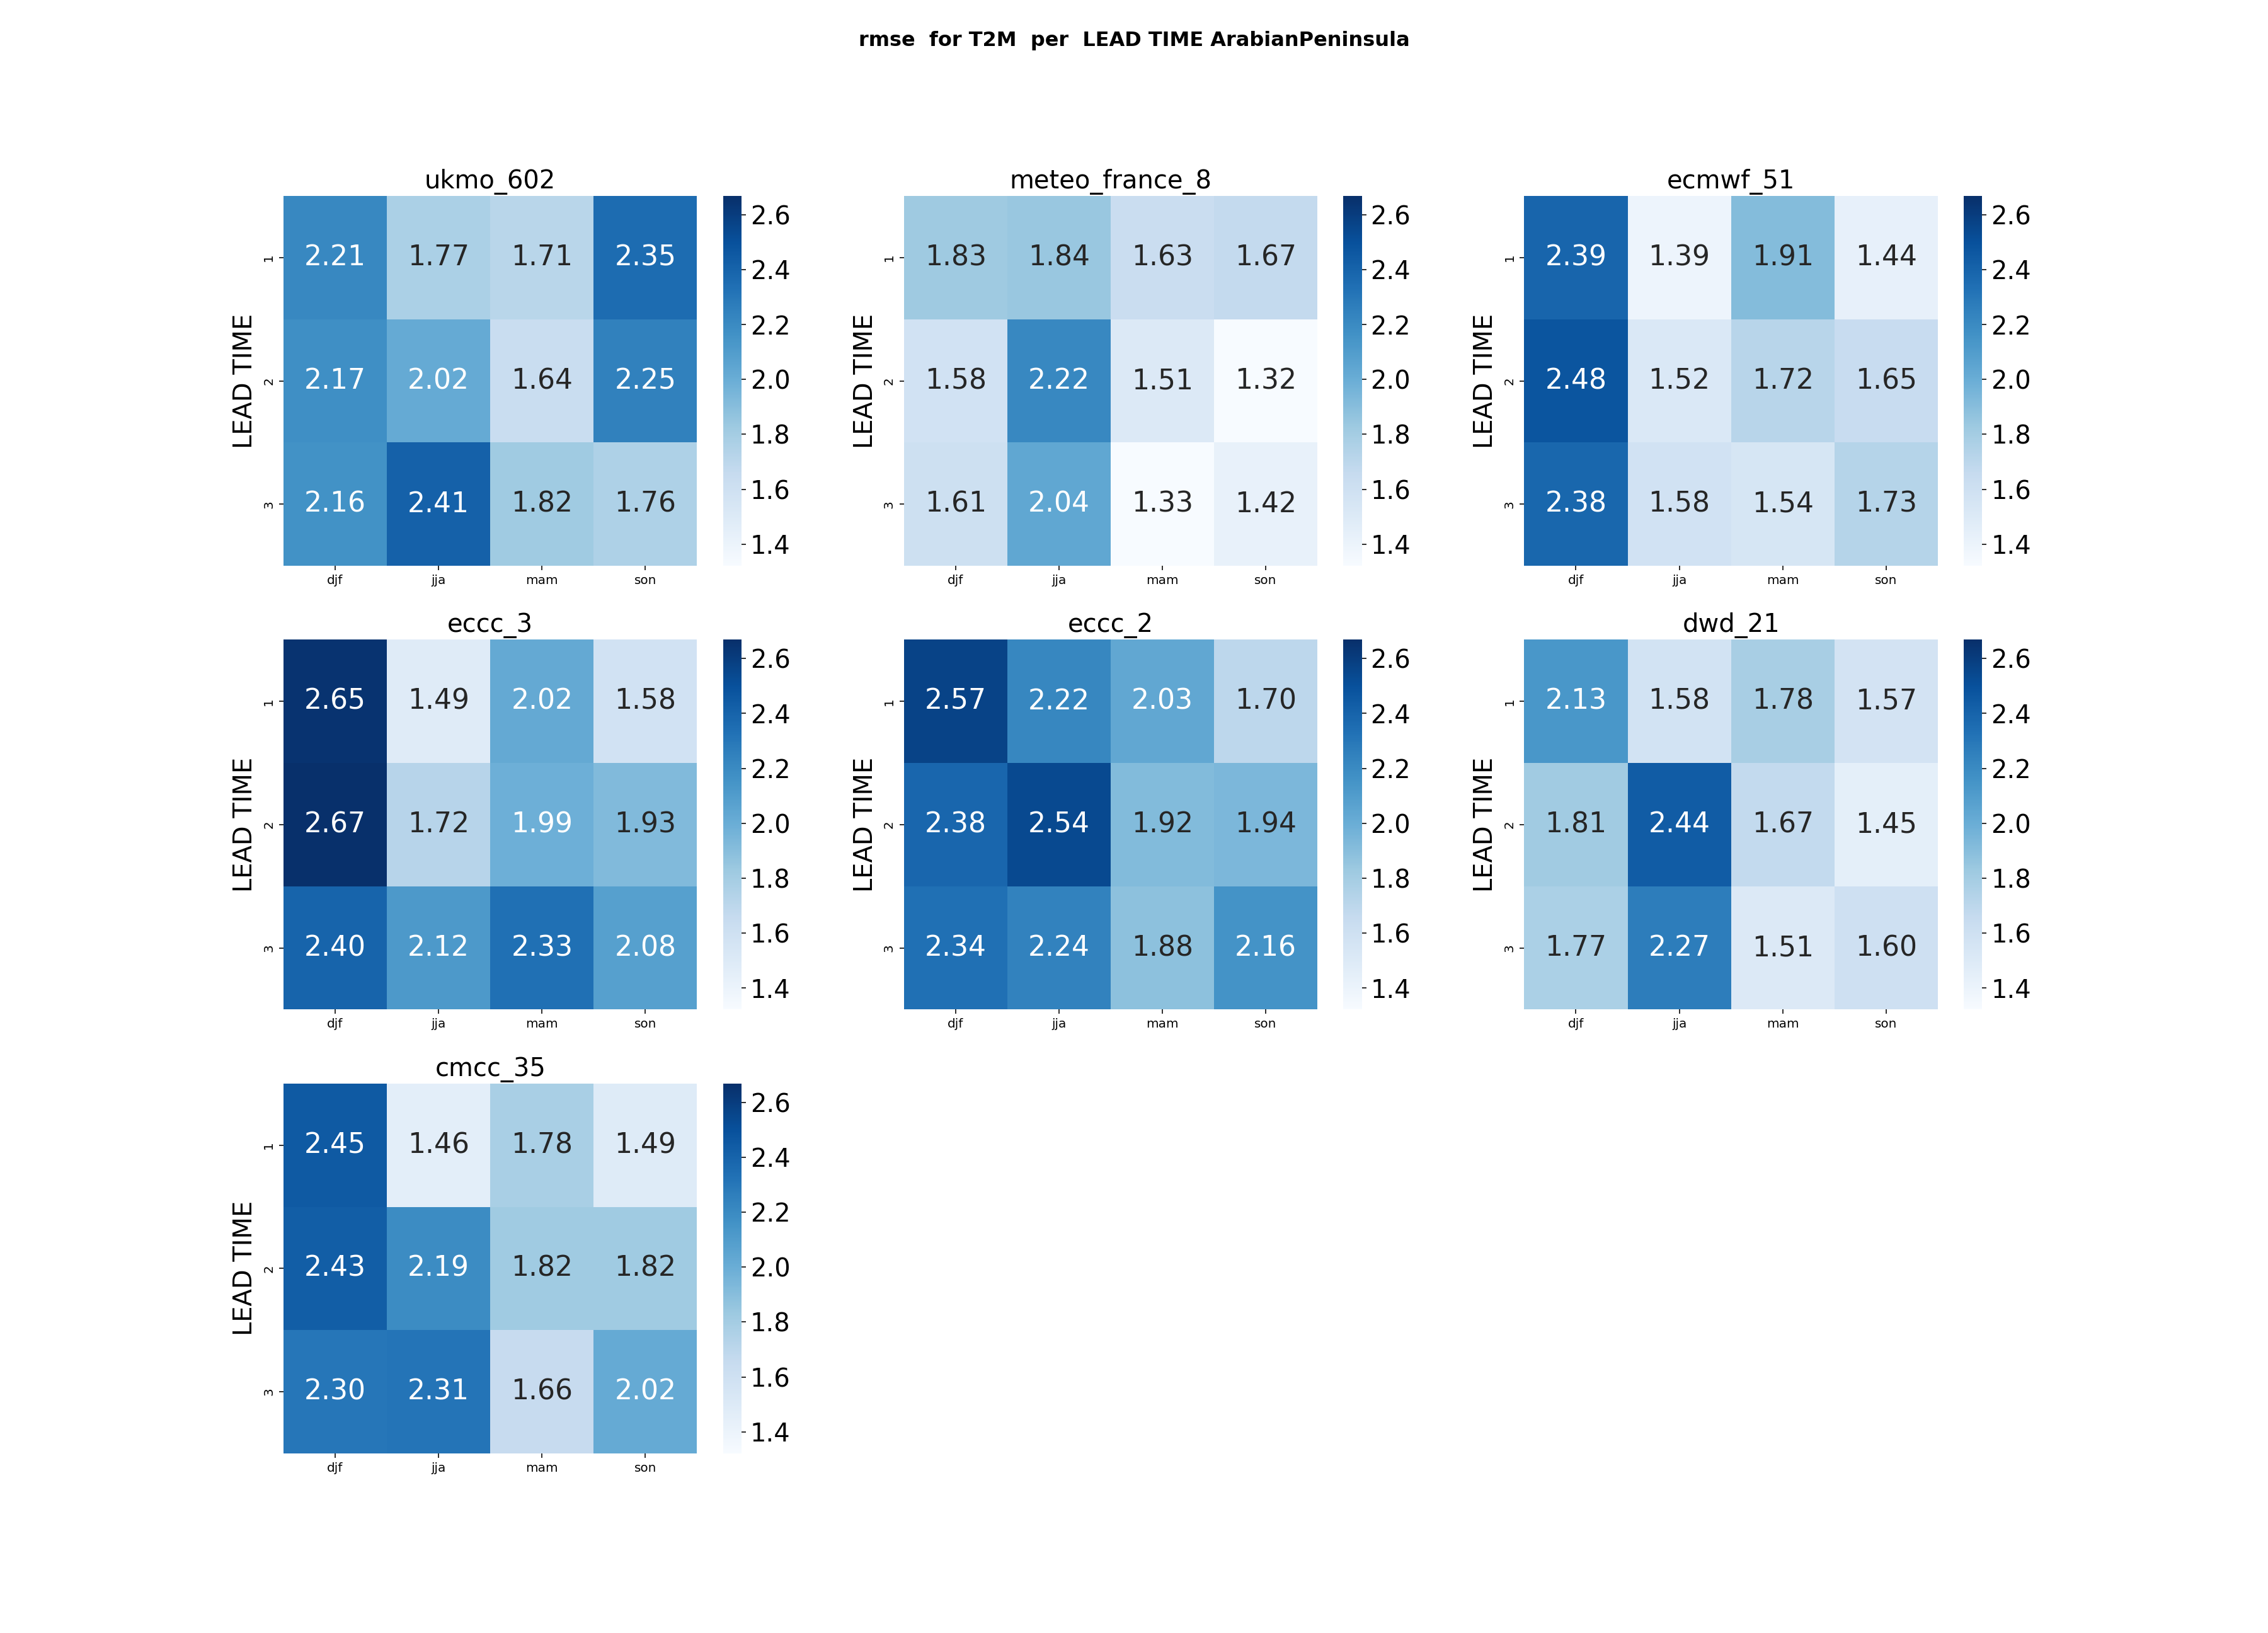
\includegraphics[scale=0.3]{plots/det/rmse/rmse_T2M_ArabianPeninsula.png}
\caption{heatmap of RMSE For T2M  (North Africa)}
\end{figure}

In the same way as North Africa, the RMSE for the Arabian Peninsula is significantly lower for \textbf{\textit{Météo-France}}, indicating superior performance.
\subsubsection{Analysis of Coefficient of Determination results}
\paragraph{focus on North Africa}

Focusing on North Africa, \textbf{\textit{ECMWF}} maintains its position as the most reliable center, consistent with its performance across the broader MENA region.
\begin{figure}[H]
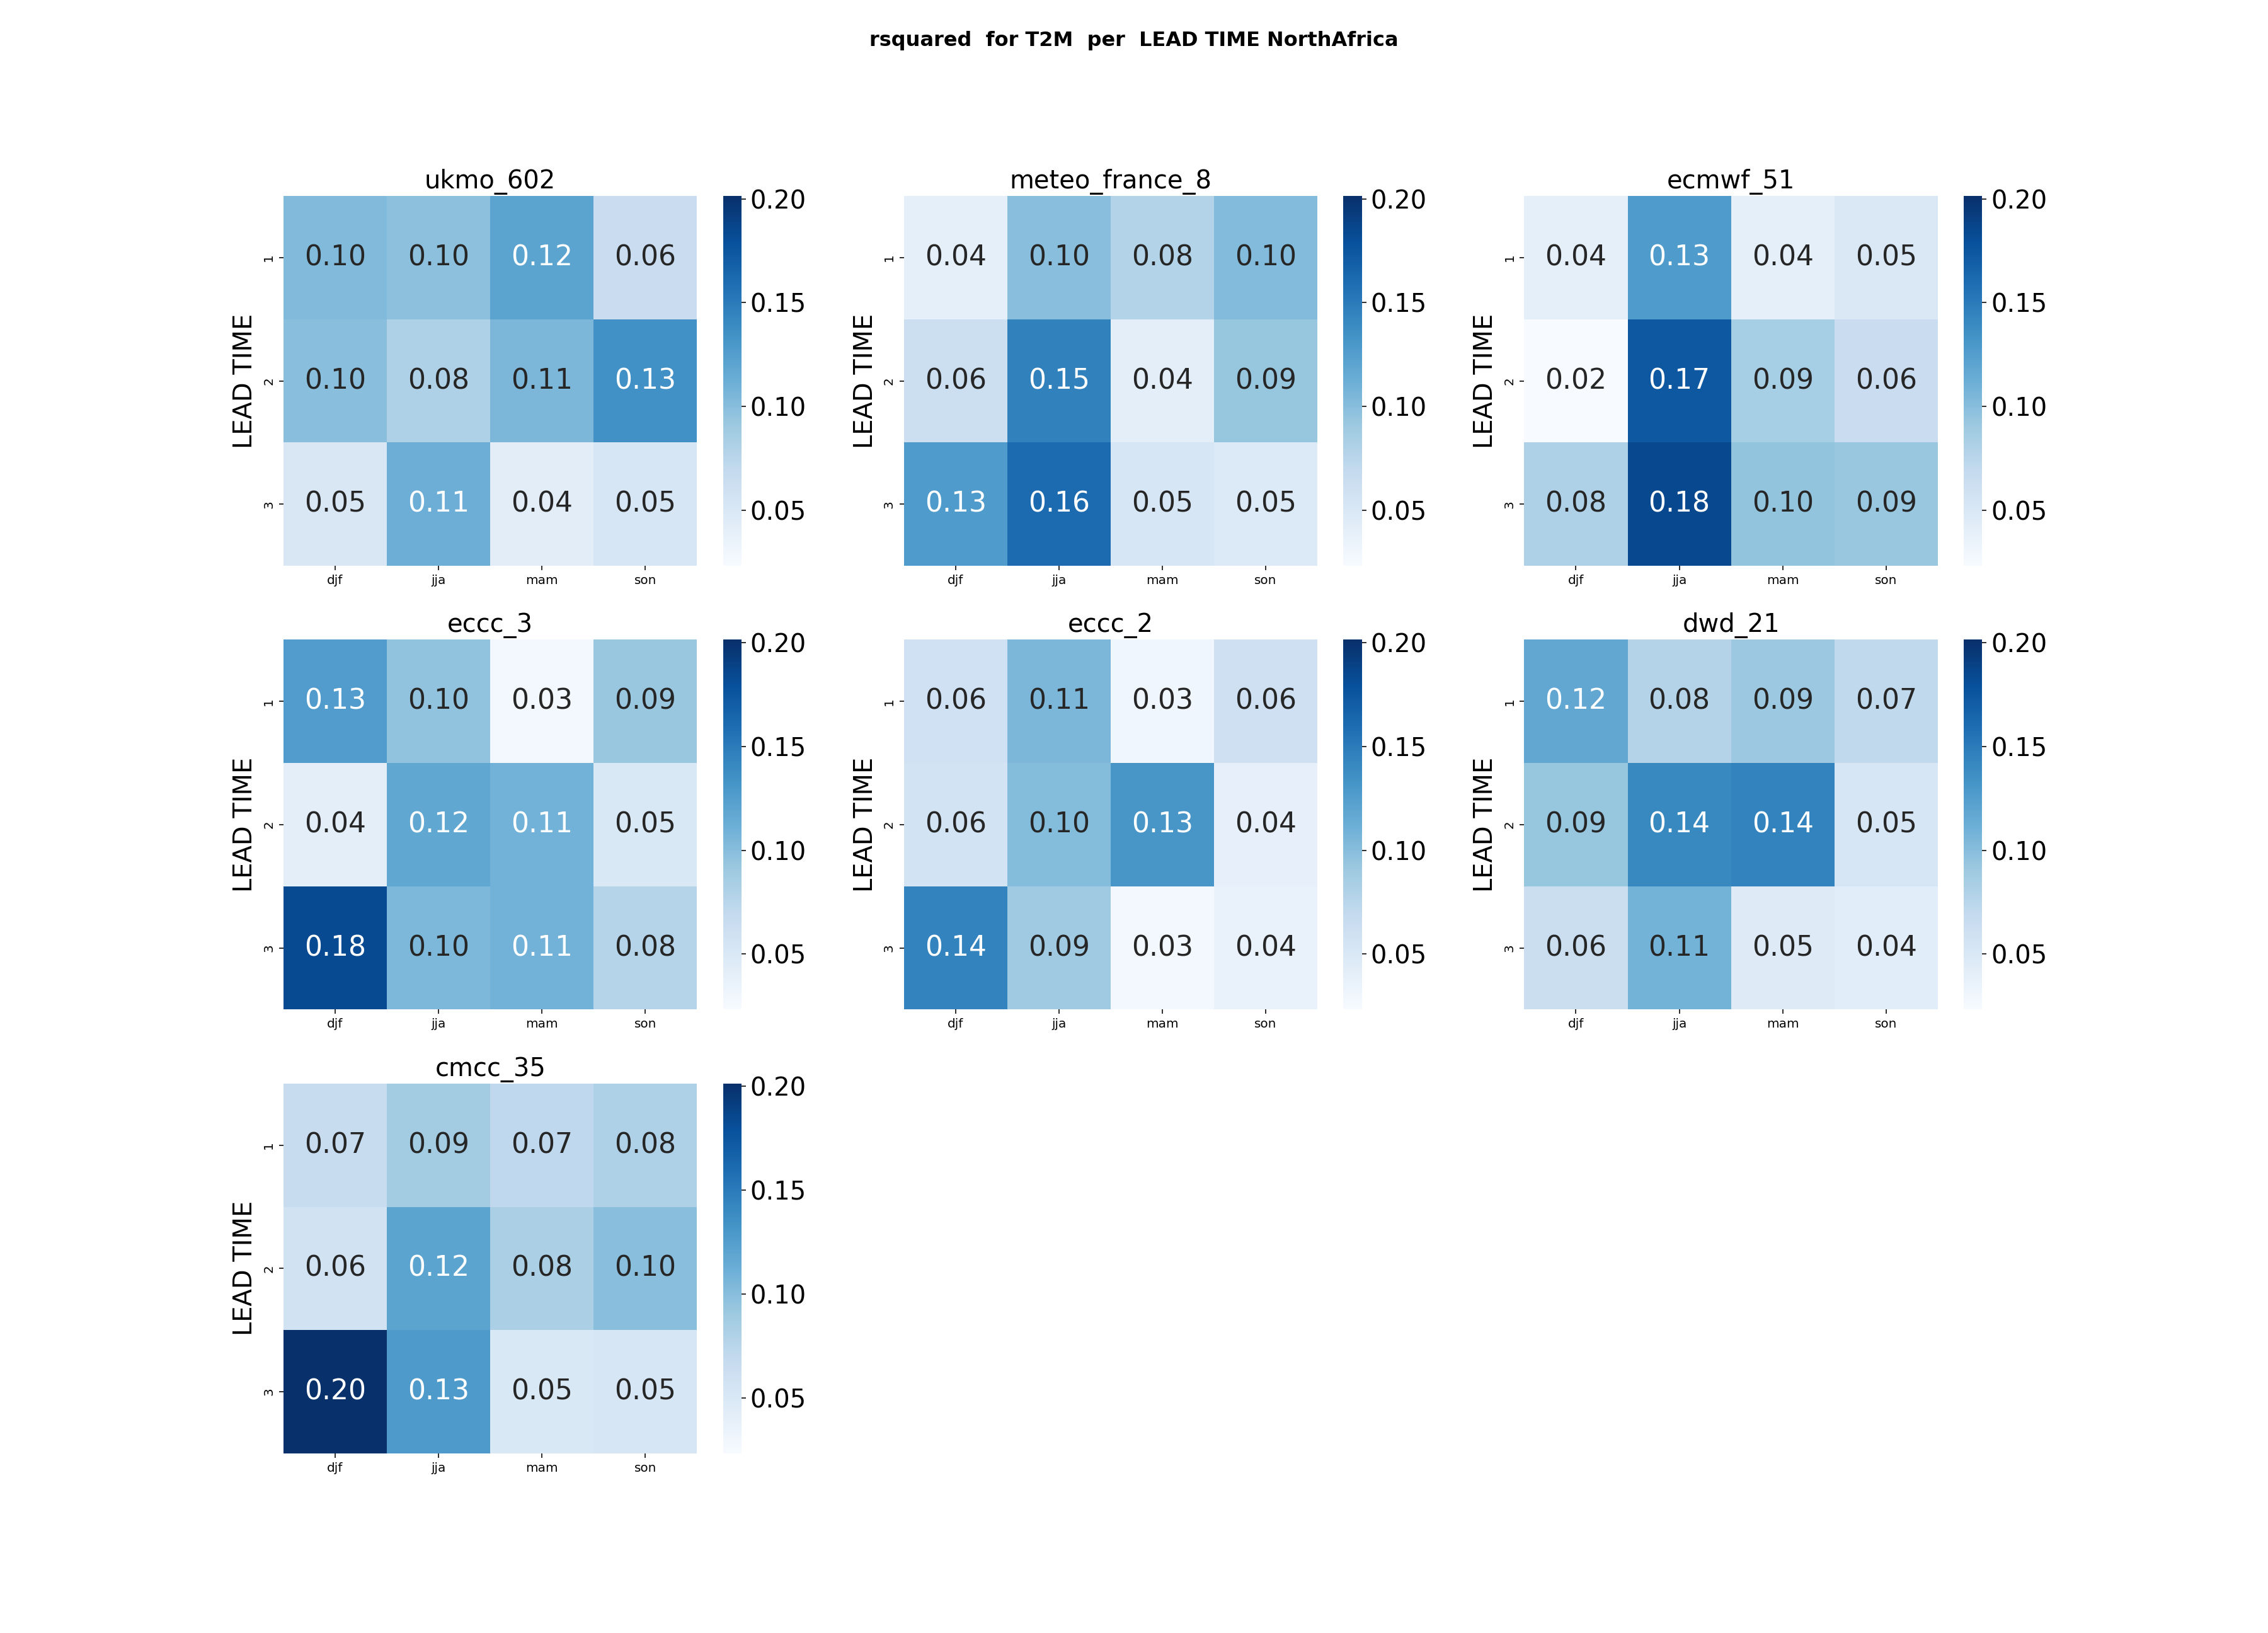
\includegraphics[scale=0.3]{plots/det/rsquared/rsquared_T2M_NorthAfrica.png}
\caption{Heatmap of T2M  RSQUARED in North Africa Region for all centers }
\end{figure}


\vspace{1.5cm}
\paragraph{focus on Arabian Peninsula}:


\begin{figure}[H]
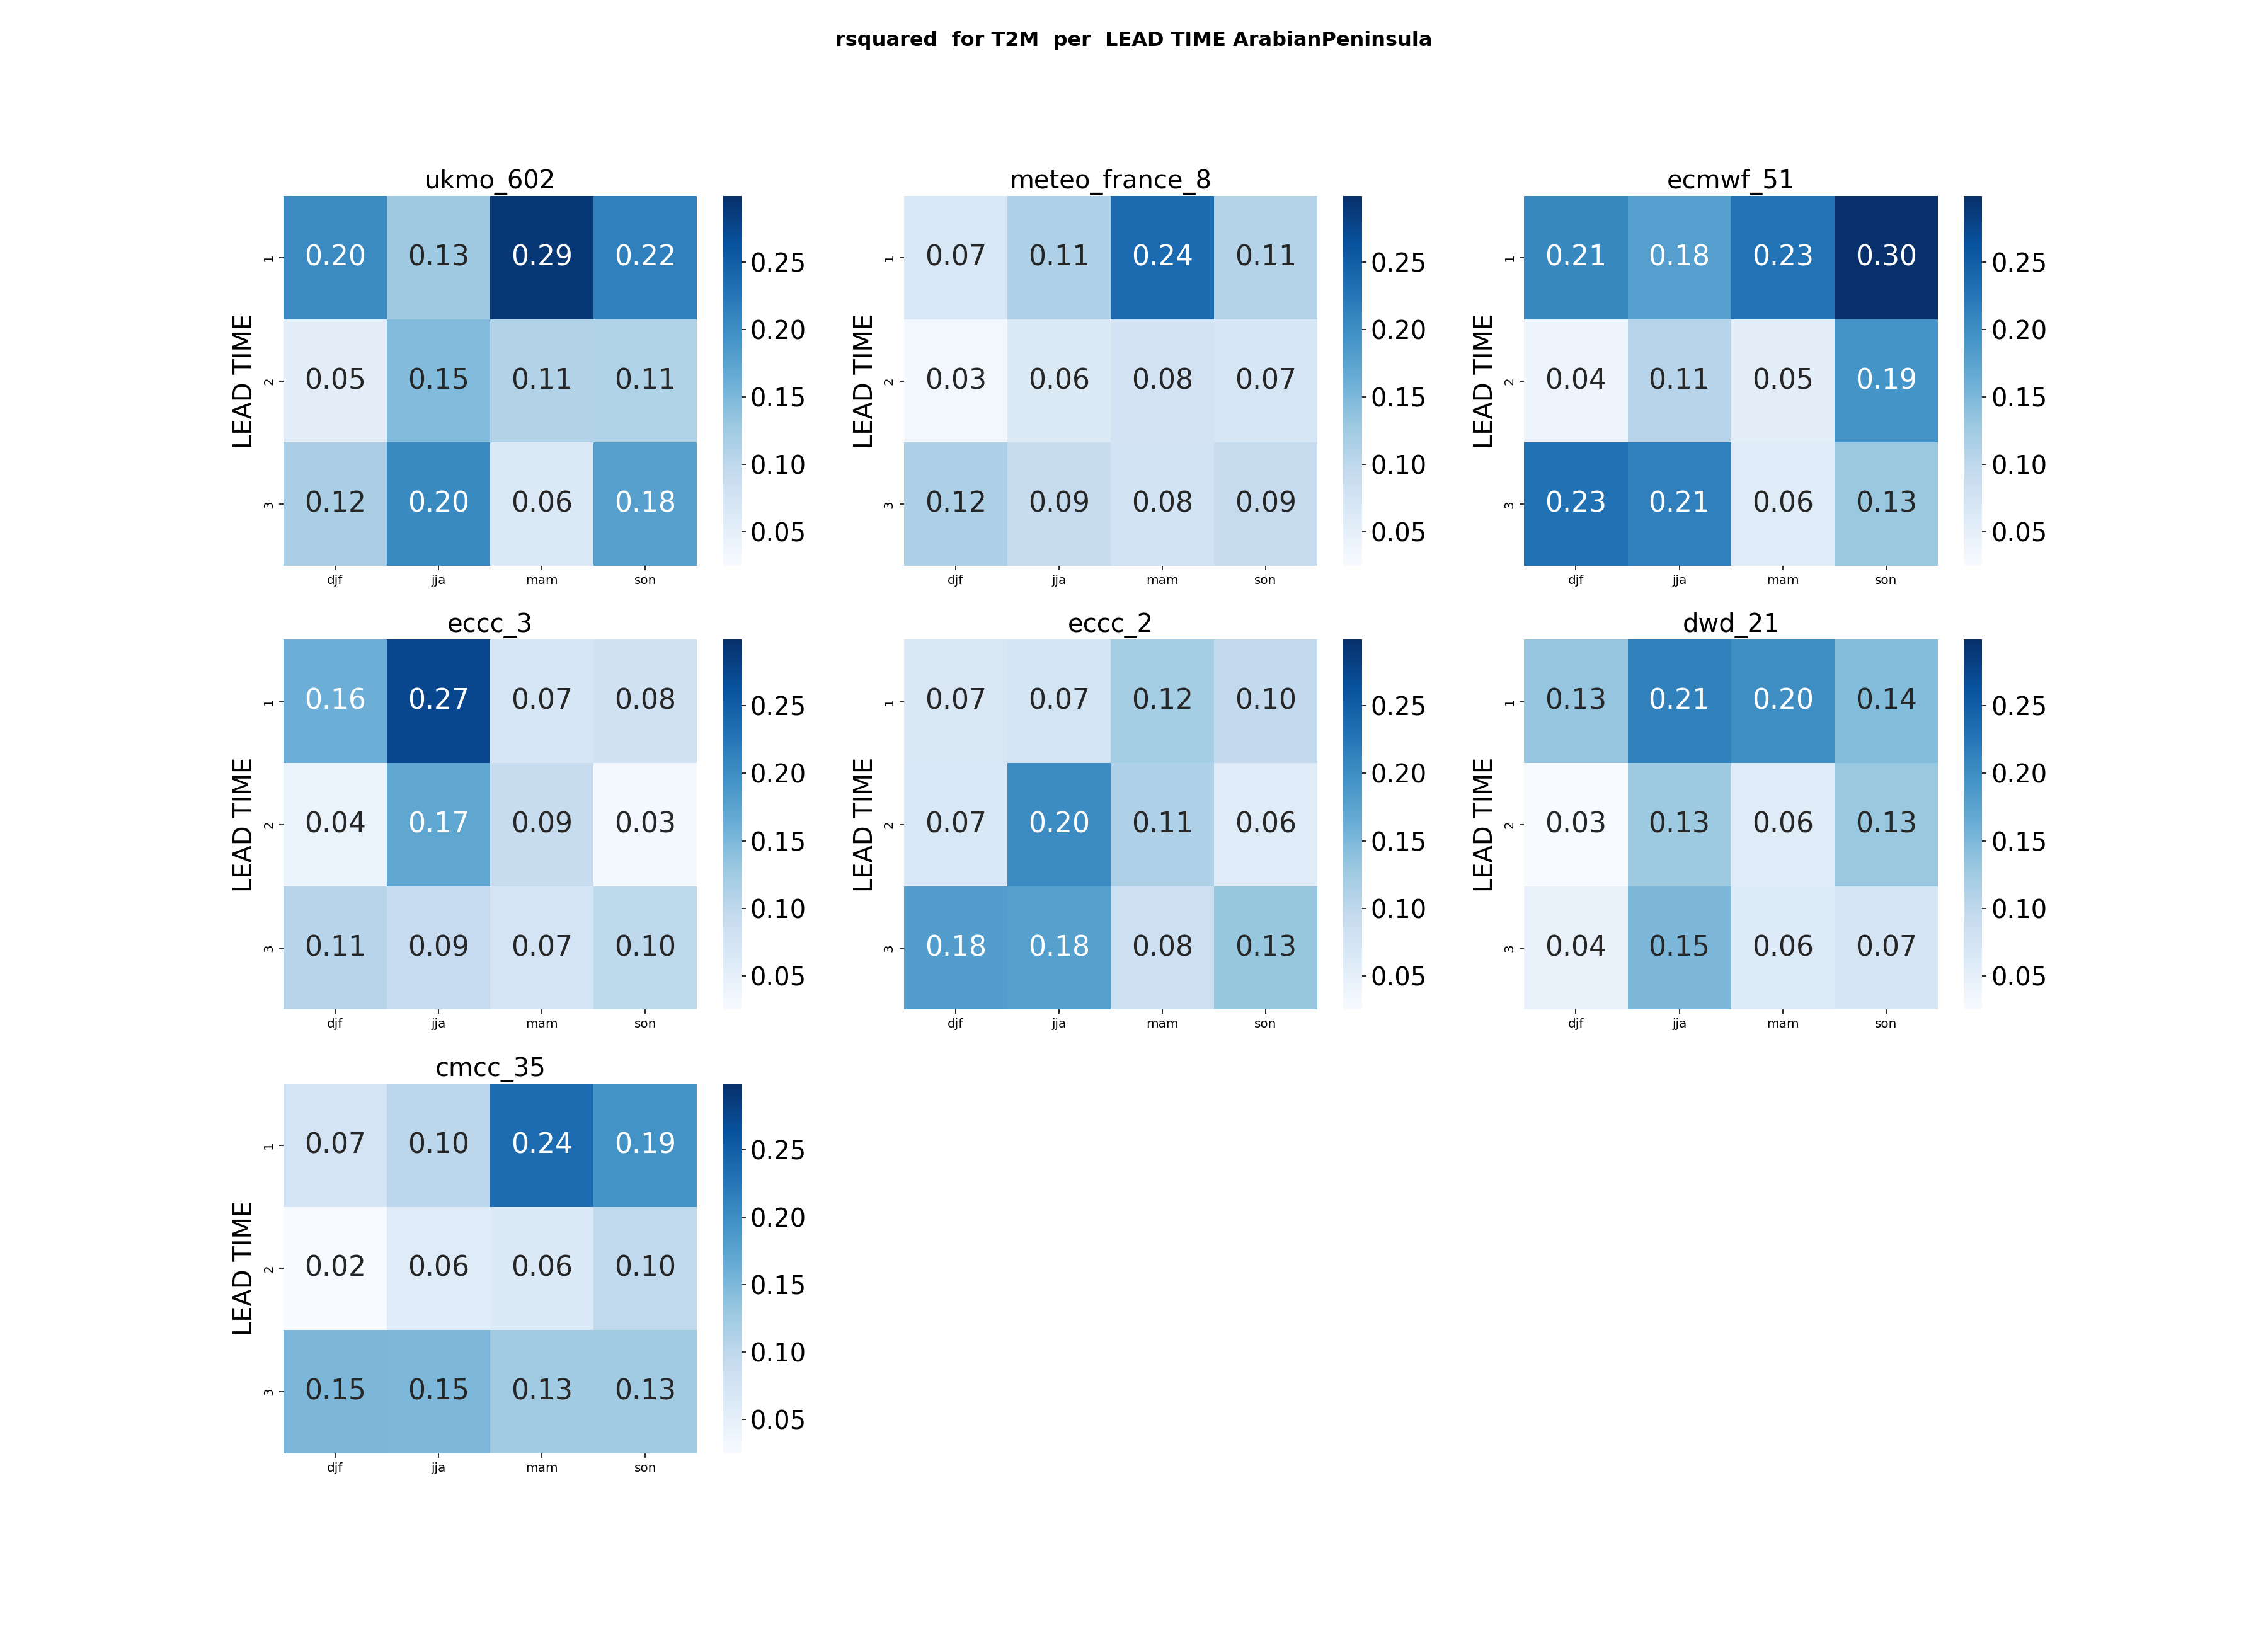
\includegraphics[scale=0.3]{plots/det/rsquared/rsquared_T2M_ArabianPeninsula.png}
\caption{Heatmap of T2M  RSQUARED in MENA Region for all centers Arabian Peninsula}
\end{figure}

the R-SQUARED for the Arabian Peninsula shows a little improvement.

\subsection{Probabilistic Evaluation Metrics}

\subsubsection{Analysis of The Brier Score results}

\paragraph{focus on North Africa}:

To evaluate model performance in North Africa, Brier Score analysis confirms that \textbf{\textit{ECMWF, CMCC, and Météo-France}} maintain low scores, reflecting consistent reliability across lead times and seasons. These findings indicate that North Africa’s unique climatic variability does not significantly impact the predictive skill of these models, affirming their adaptability within the broader MENA region. Minimal score variations across lead times further emphasize their robustness for accurate probabilistic forecasting over varying temporal ranges.

\begin{figure}[H]
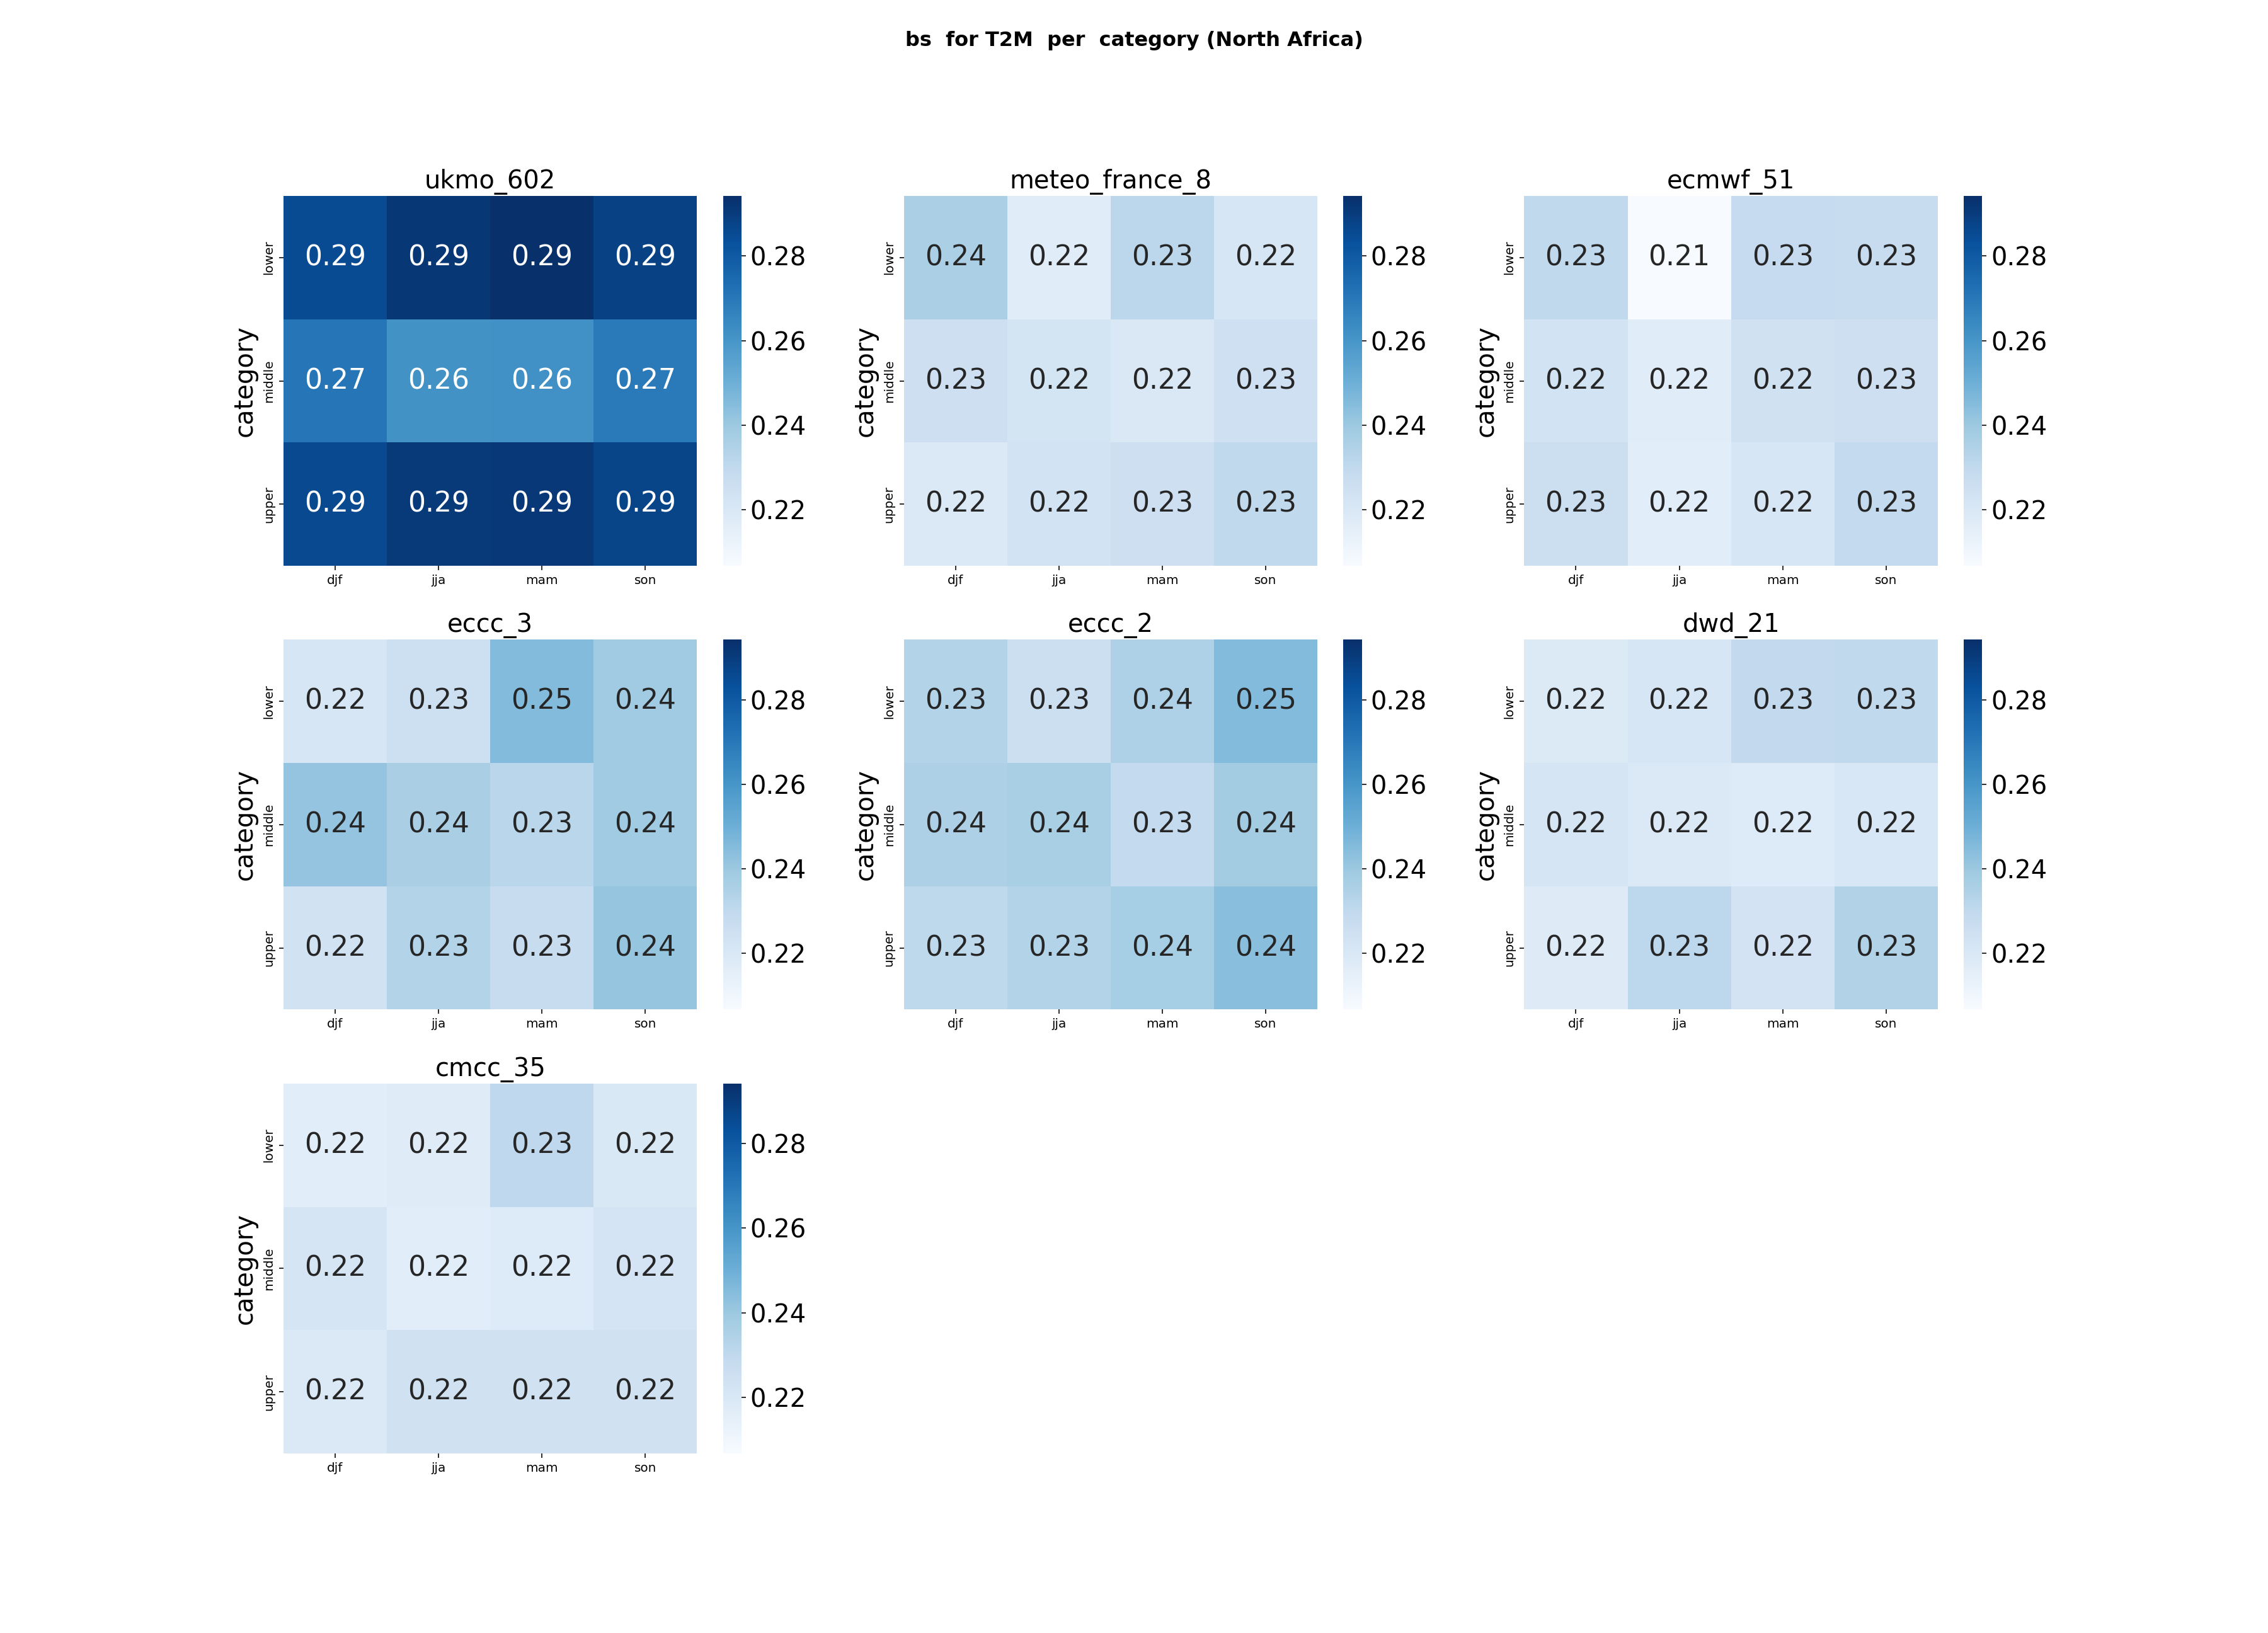
\includegraphics[scale=0.3]{plots/prob/bs/bs_T2M_category_NorthAfrica.png}

\caption{Heatmap of T2M  brier score for all centers in North Africa region}
\end{figure}





\vspace{1.5cm}
\paragraph{focus on Arabian Peninsula}:
there is no big difference in North Africa.
\subsubsection{Analysis of Reliability results}
\paragraph{focus on North Africa}:
\begin{figure}[H]
\includegraphics[scale=0.3]{plots/prob/rela/rela_T2M_NorthAfrica.png}

\caption{Heatmap of T2M  reliability  for all centers in North Africa}
\end{figure}


A more focused analysis on North Africa has not significantly altered the overall conclusions derived from the broader MENA region. The consistent performance patterns observed across the different models and seasons remain largely unchanged when examining the North African context. 

\paragraph{focus on Arabian Peninsula}:

there is no big difference in  Arabian Peninsula.
\subsubsection{Analysis of The ranked probability score results}
\paragraph{focus on north africa:}
For the North African region, the results mirror those observed in the broader MENA region.  

This suggests that despite the localized focus on North Africa, the model performance differences remain significant, particularly for UKMO. 

\begin{figure}[H]
\includegraphics[scale=0.3]{plots/prob/rps/rps_T2M_NorthAfrica.png}

\caption{Heatmap of T2M  rps  for all centers in North Africa regions}
\end{figure}


\paragraph{focus on Arabian Peninsula}:
All centers exhibit nearly identical performance, with the exception of \textit{UKMO}, which demonstrates lower skill compared to the others.
\subsubsection{Analysis of Receiver Operating Characteristic results}
\paragraph{focus on north africa:}
\begin{figure}[H]
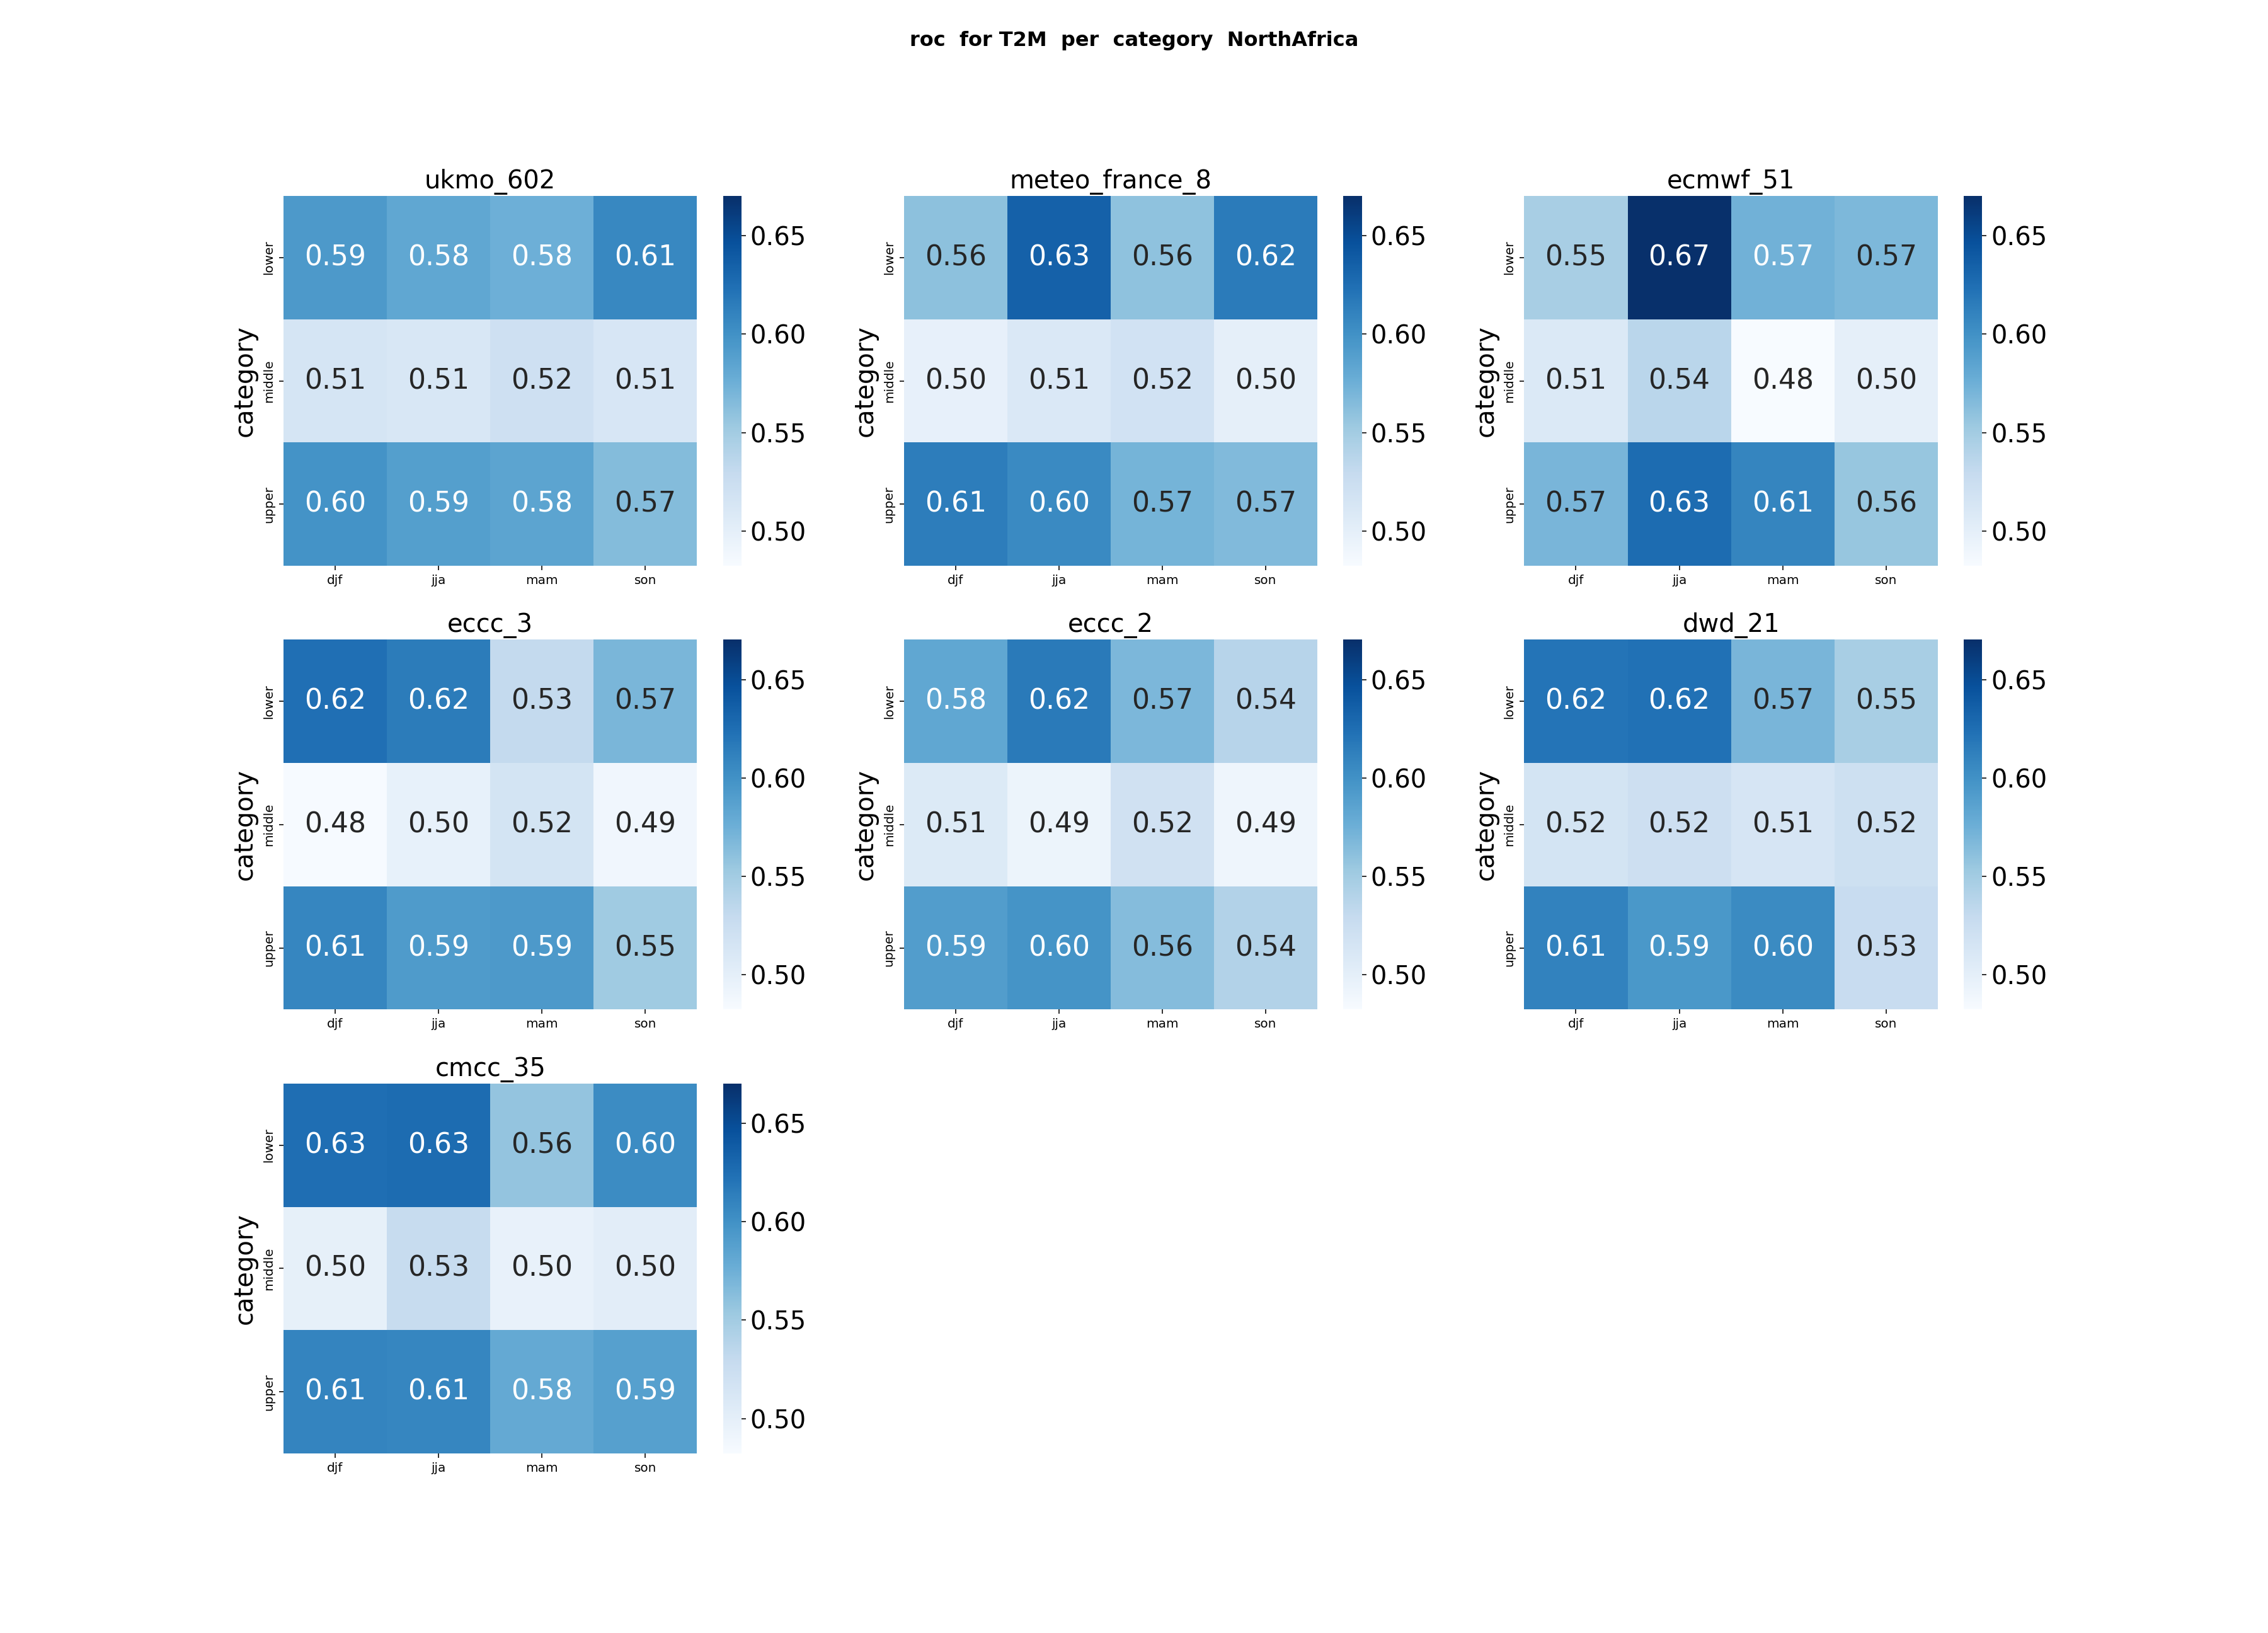
\includegraphics[scale=0.3]{plots/prob/roc/roc_T2M_category_NorthAfrica.png}

\caption{Temperature AUC  heatmaps for north africa }
\end{figure}

The figure above confirms the same conclusions for the North Africa region. The models generally maintain similar performance, with high AUC values reflecting strong discrimination skill across all categories. UKMO continues to show robust results in terms of ROC, despite its weaker reliability performance. As observed previously, the "middle" probability category remains the least performant compared to the "lower" and "upper" categories, indicating the models' reduced ability to predict moderate probability events. This consistency in findings suggests that the regional focus on North Africa does not significantly alter the overall assessment of model performance.
\paragraph{focus on Arabian Peninsula}:
There are no significant differences in performance across the centers, indicating comparable skill levels.
\subsubsection{Analysis of Relative operating characteristics Skill Score results }
\paragraph{focus on north africa:}
The ROC Skill Score (ROCSS) analysis reveals similar conclusions to the ROC results for Mena region and north Africa. 
\begin{figure}[H]
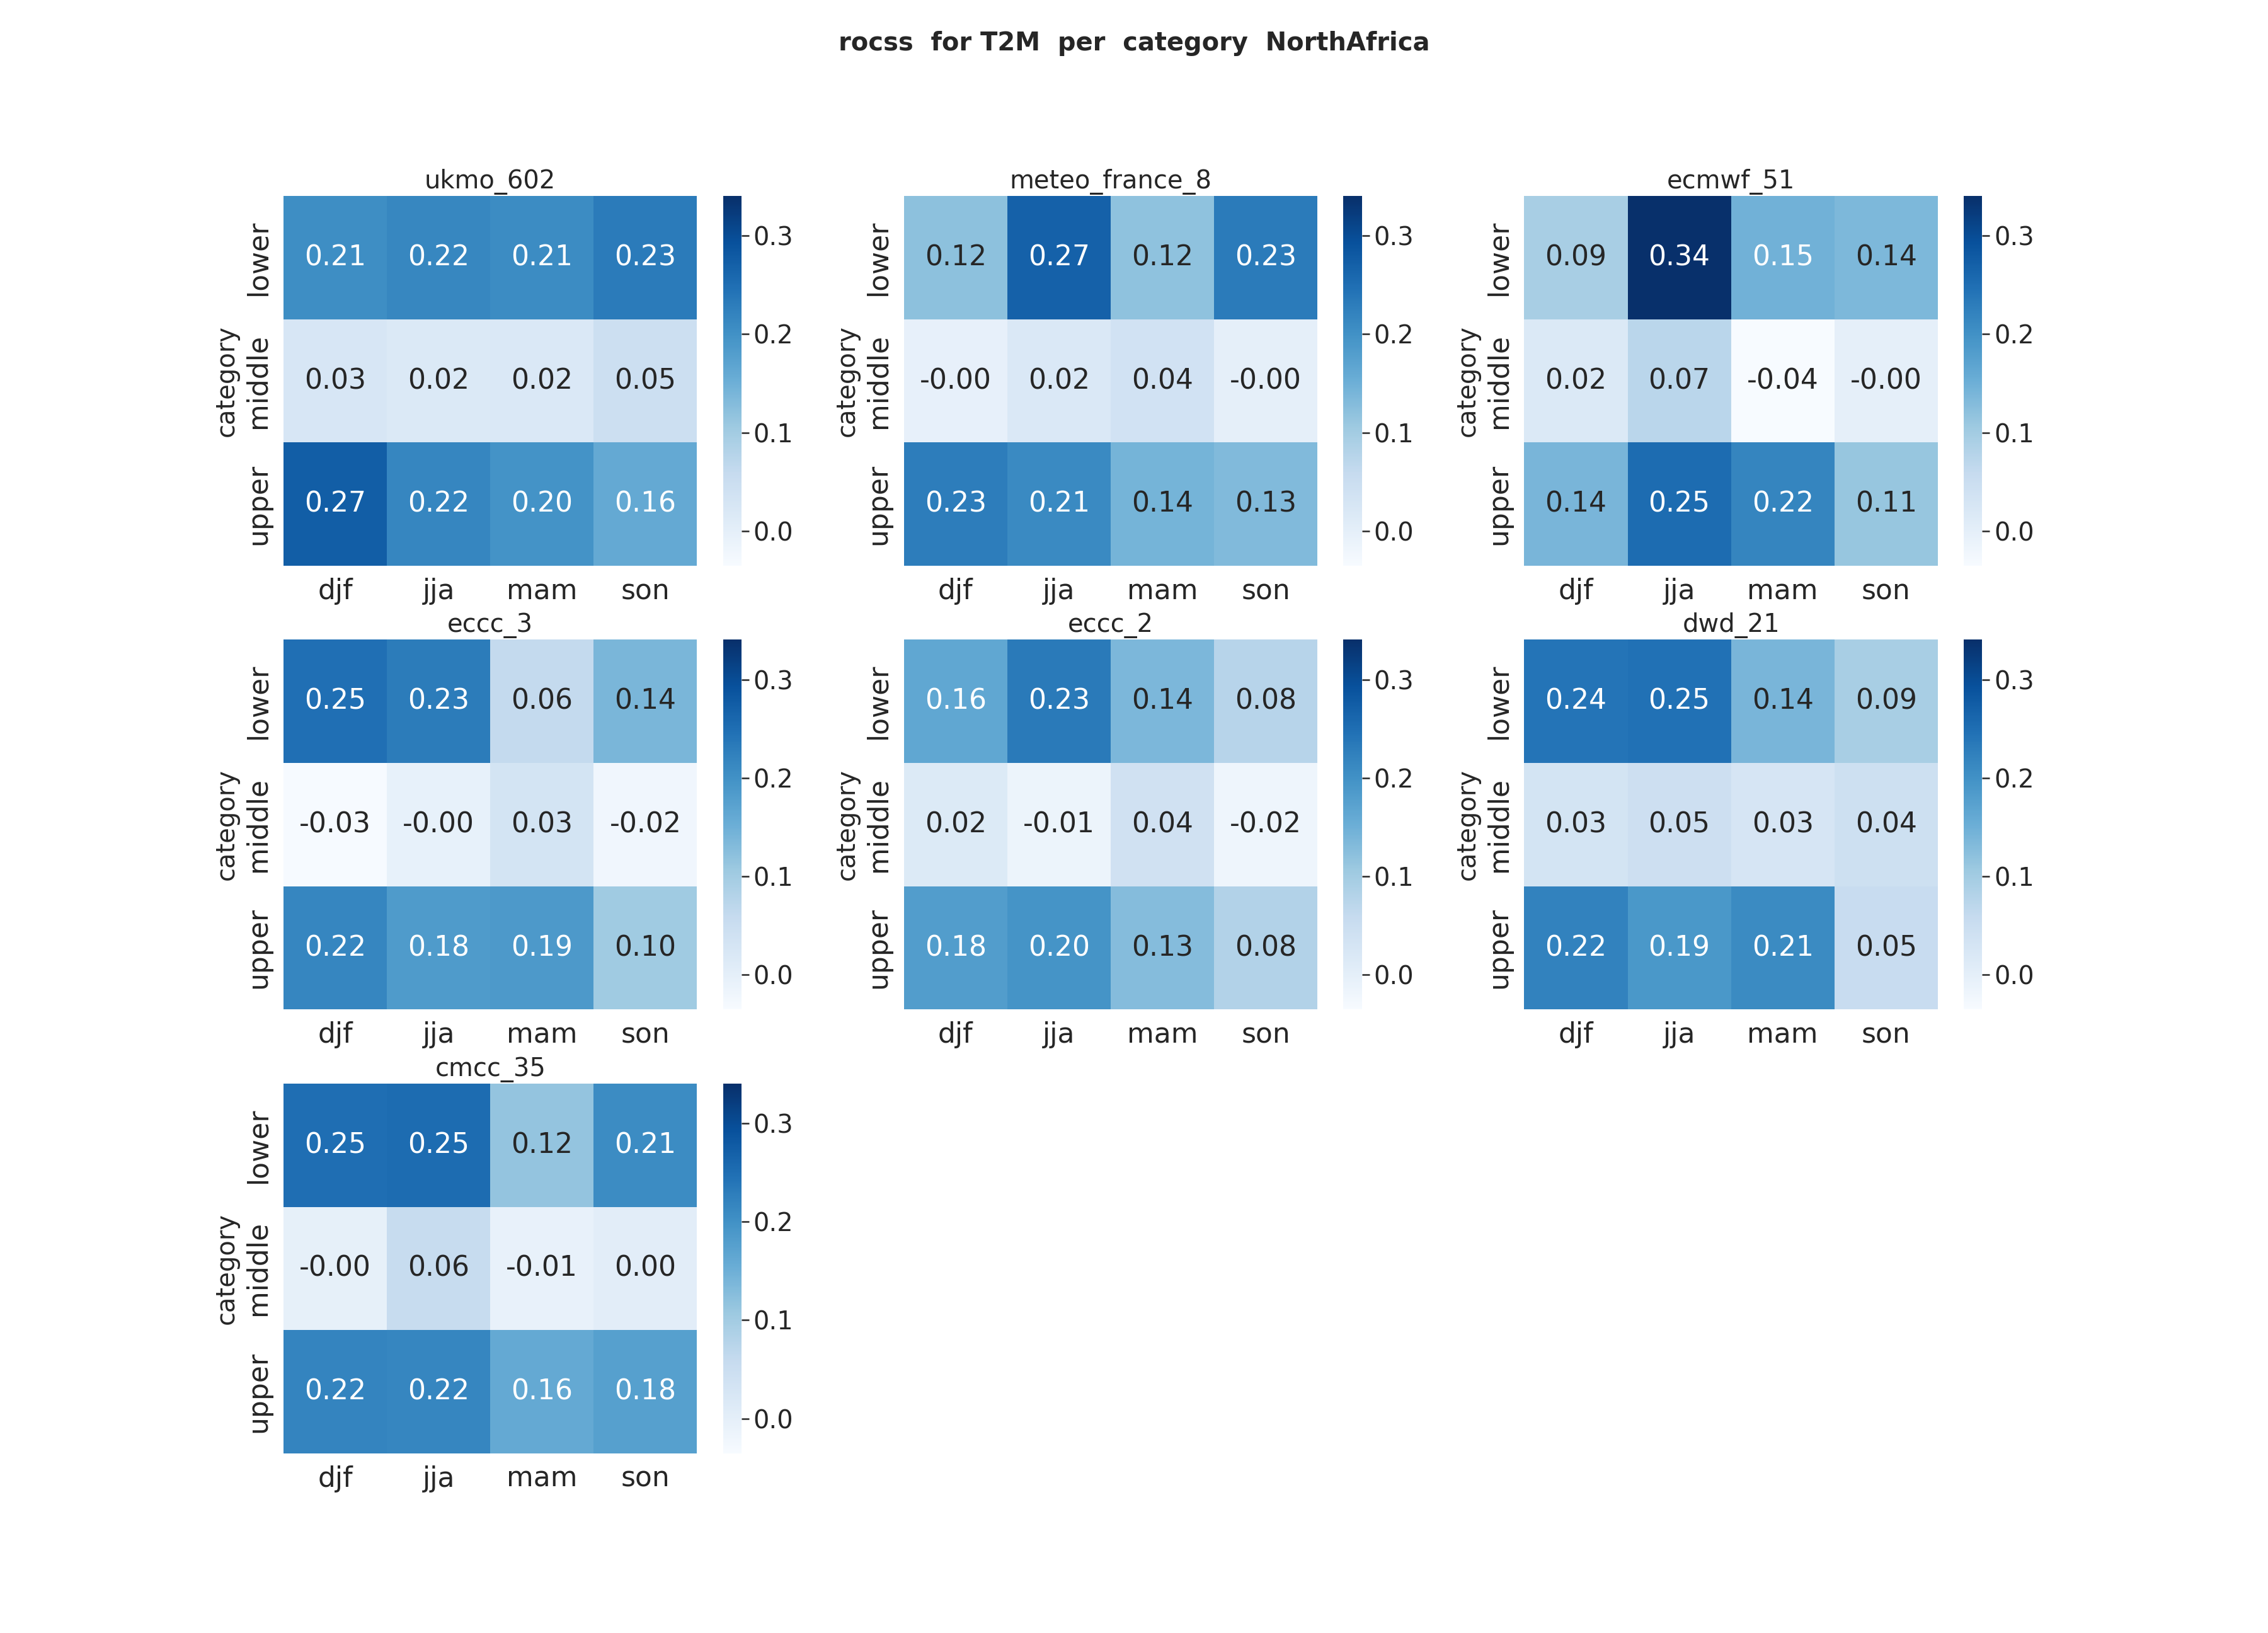
\includegraphics[scale=0.3]{plots/prob/rocss/rocss_T2M_category_NorthAfrica.png}

\caption{Temperature ROCSS  heatmaps for north africa }
\end{figure}

\paragraph{focus on Arabian Peninsula}:
There are no significant differences



\section{precipitation}
\subsection{Deterministic Evaluation Metrics}
\subsubsection{Analysis of ACC results}
 
the Arabian Peninsula. As for North Africa, theb\textbf{\textit{meteo-france}} shows good acc.
\vspace{1.5cm}

\paragraph{focus on north africa:}
according to the heatmap below, the correlation shows no big difference for the first lead-time, but for the second and third lead-times, it became lower. Thus, the \textbf{\textit{ecmwf,ukmo and meteo-france}} maintain relatively good correlation.


\begin{figure}[H]
	\centering
	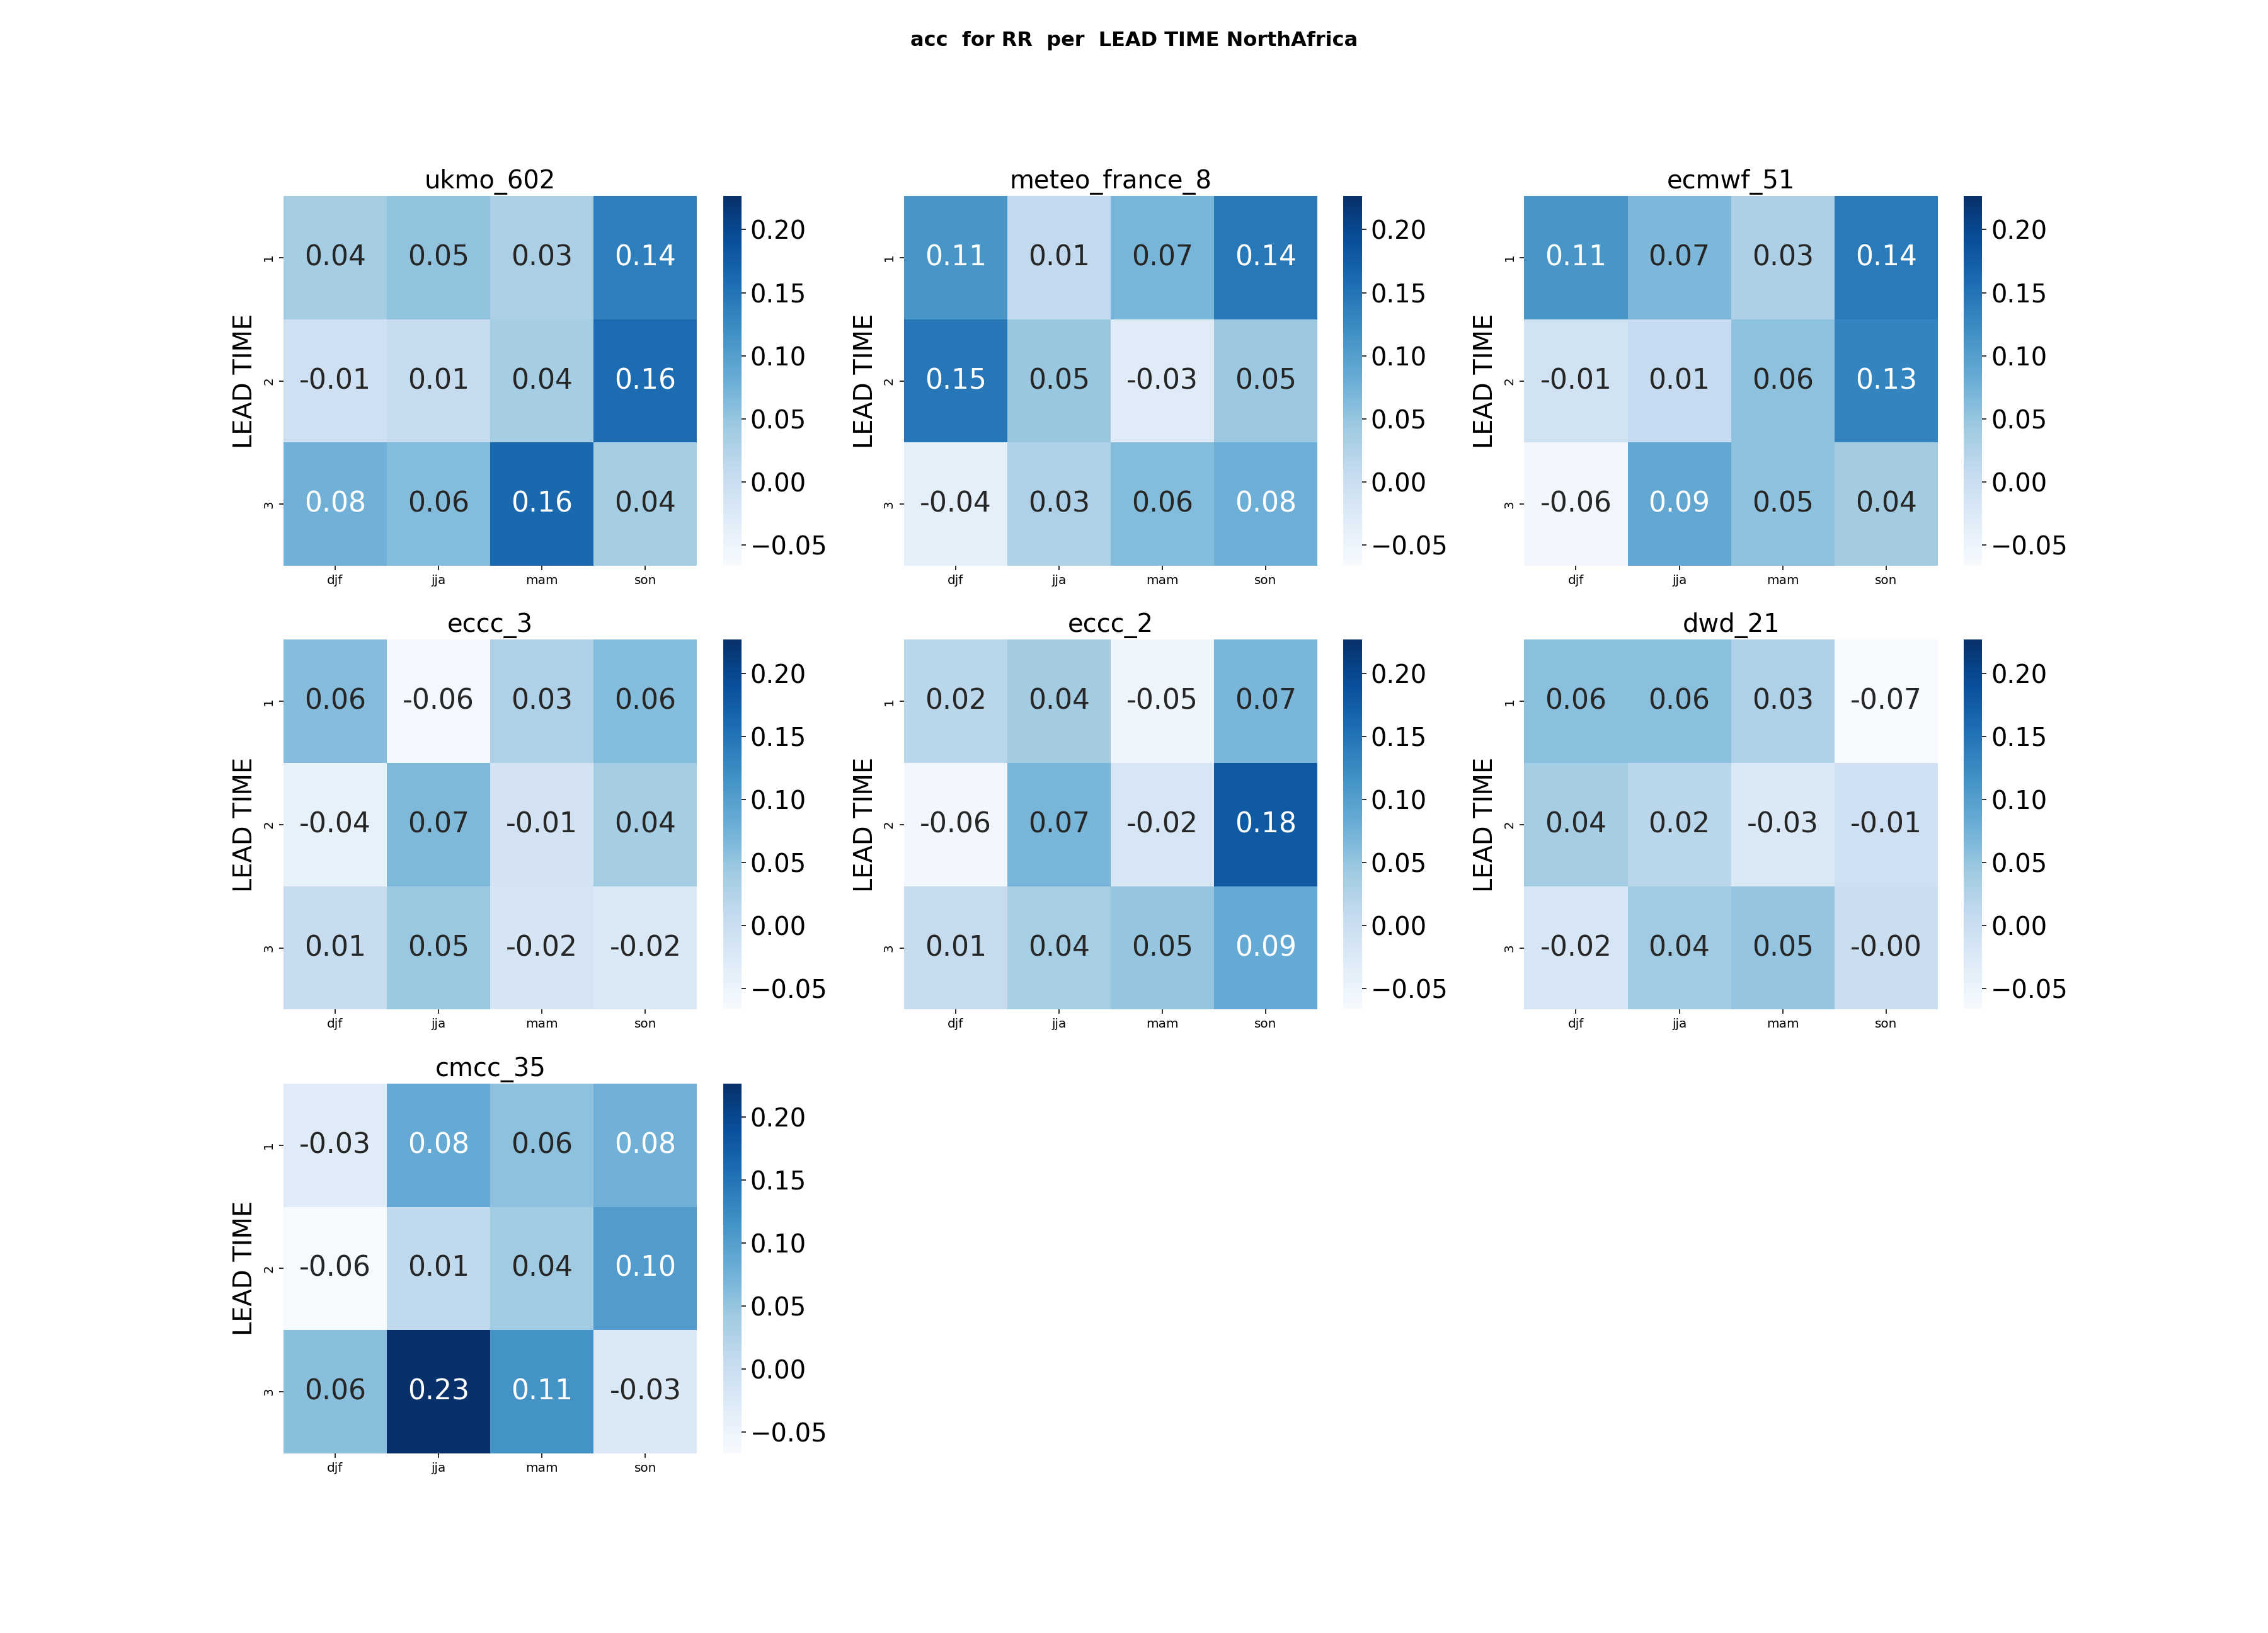
\includegraphics[scale=0.25]{plots/det/acc/acc_RR_NorthAfrica.png}
	\caption{The Heatmap of ACC for the North Africa region for every period \textbf{\textit{(1 for perfect Correlation)} }}
\end{figure}

\vspace{1.5cm}
\paragraph{focus on Arabian Peninsula}:

\begin{figure}[H]
	\centering
	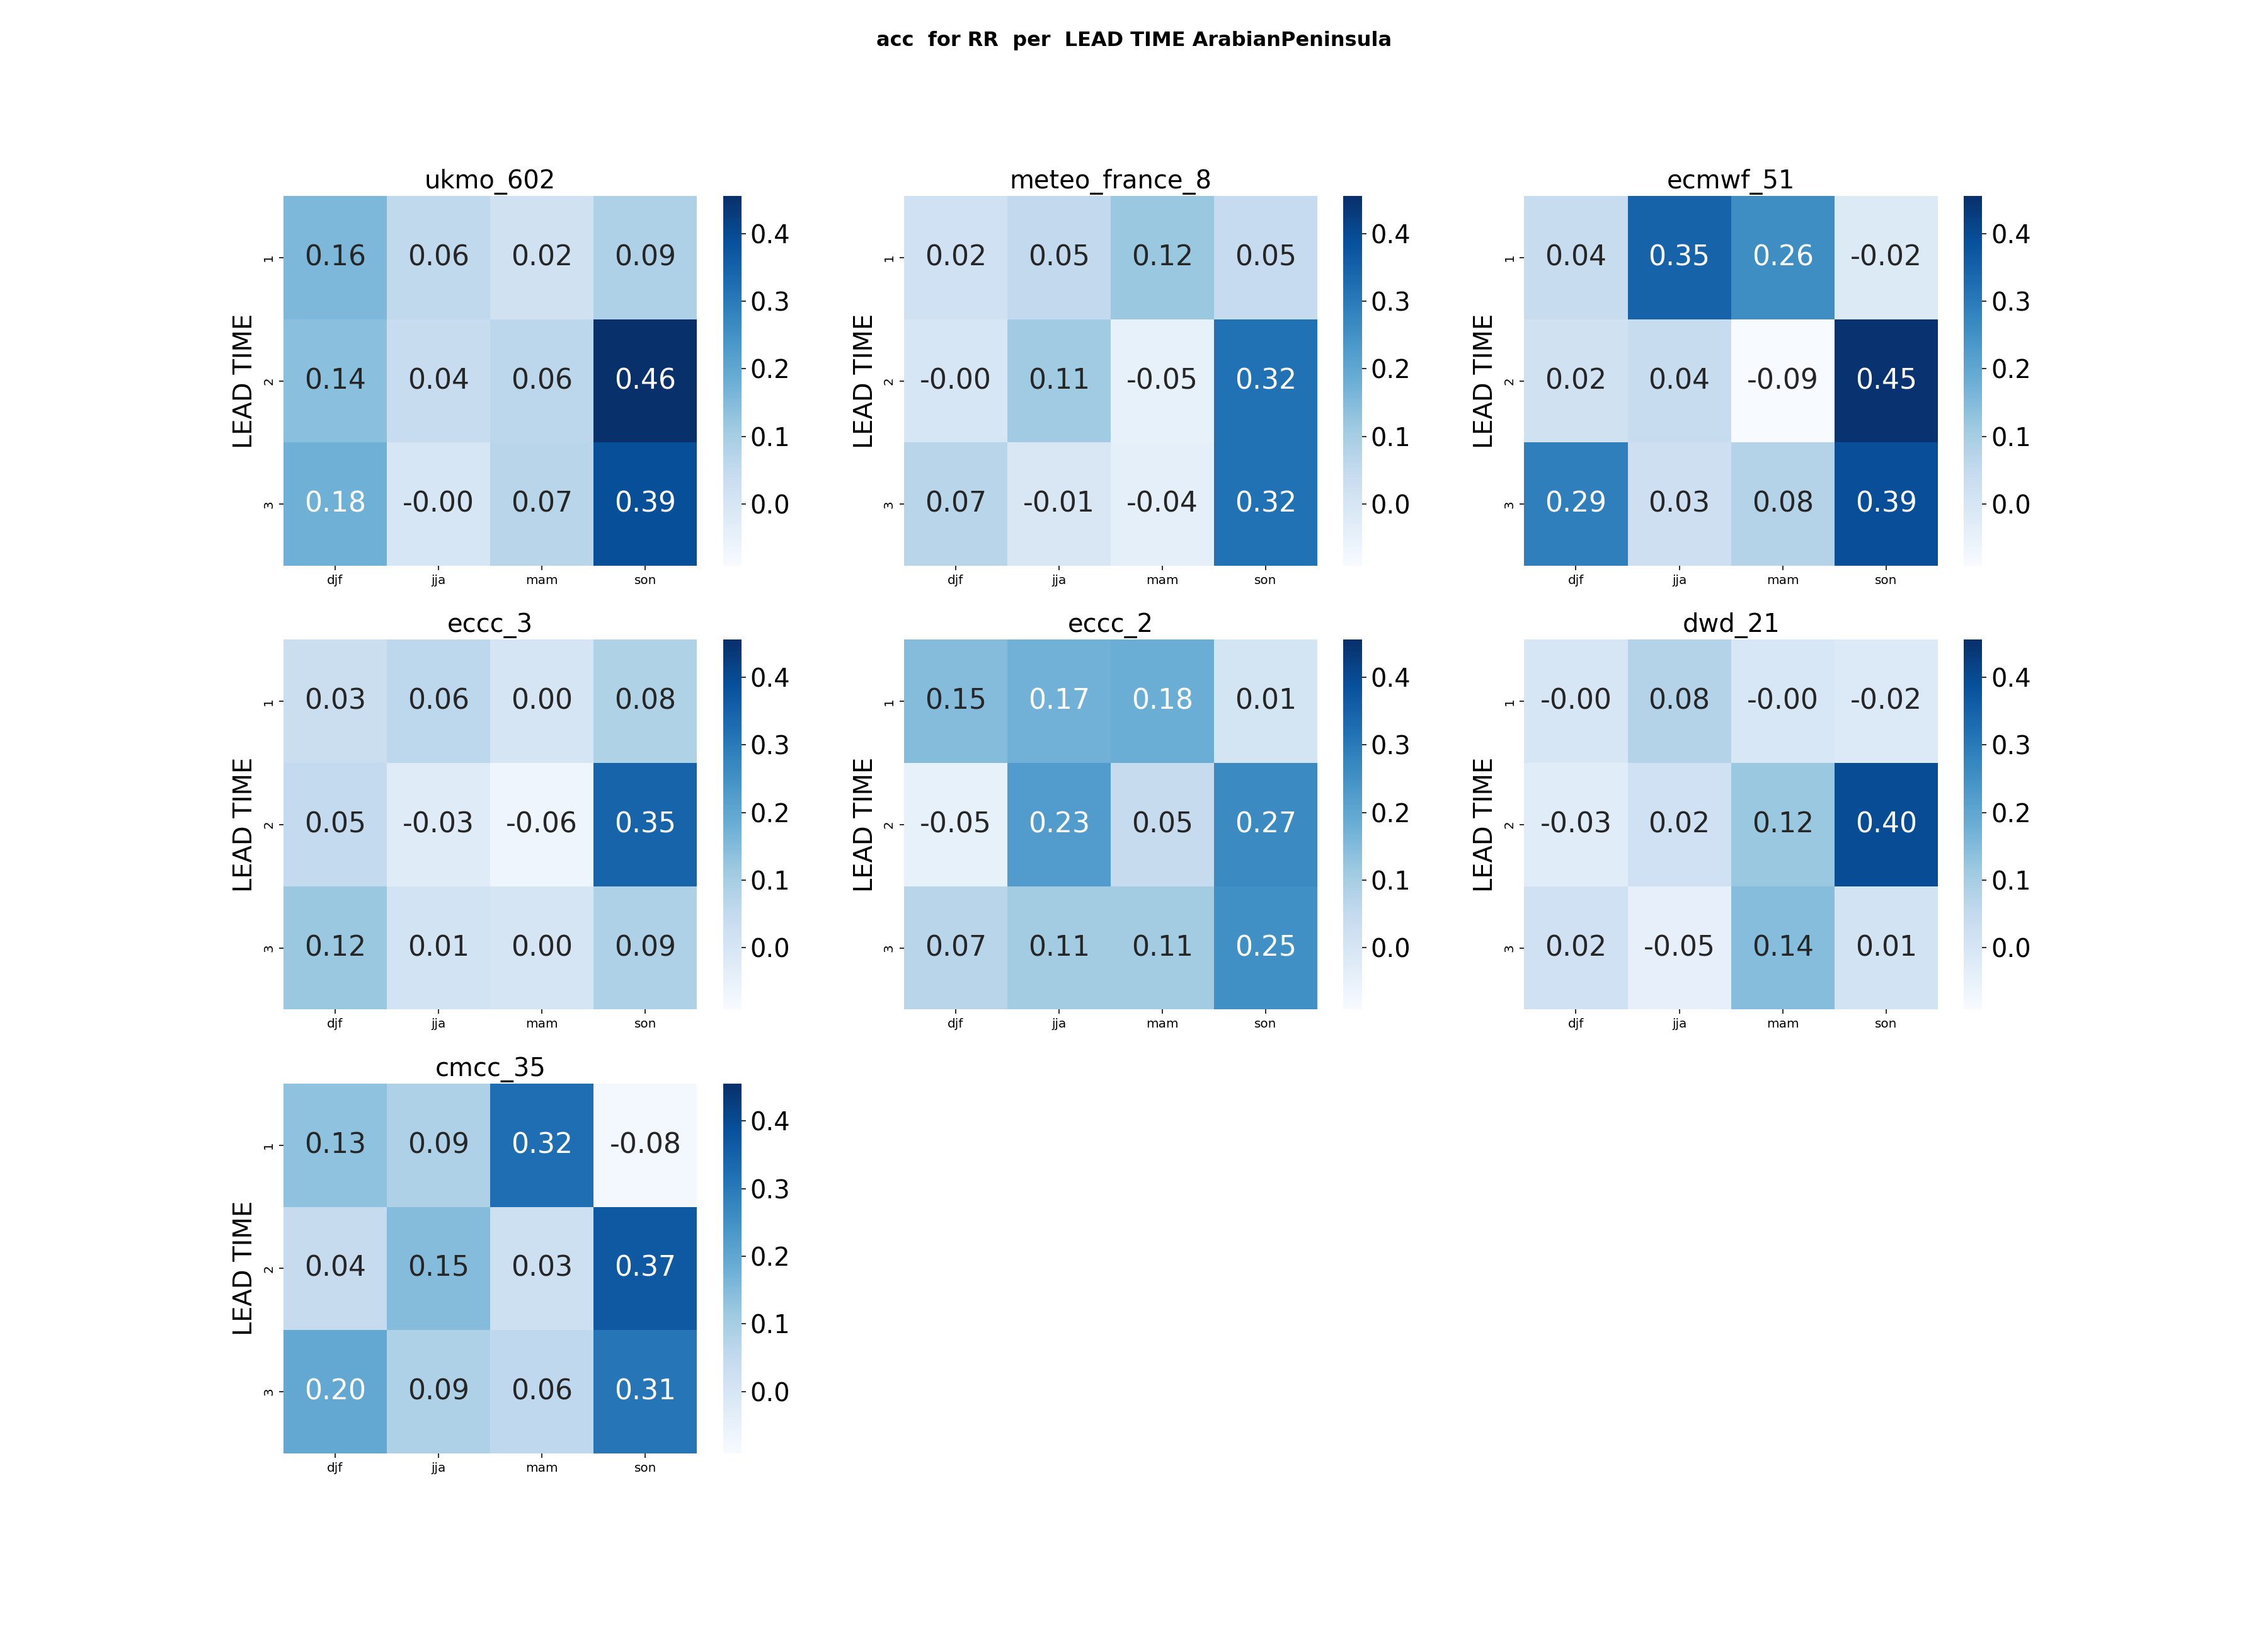
\includegraphics[scale=0.25]{plots/det/acc/acc_RR_ArabianPeninsula.png}
	\caption{The Heatmap of acc for the mena region for every period \textbf{\textit{(1 for perfect Correlation)} }}
\end{figure}

The analysis of the Arabian Peninsula shows that the score is much better than the general situation of the mena region. The acc is good especially for SON for the second and third lead-times.
\subsubsection{Analysis of RMSE Results}

\vspace{1.5cm}

\paragraph{focus on North Africa} : 
\begin{figure}[H]
\centering
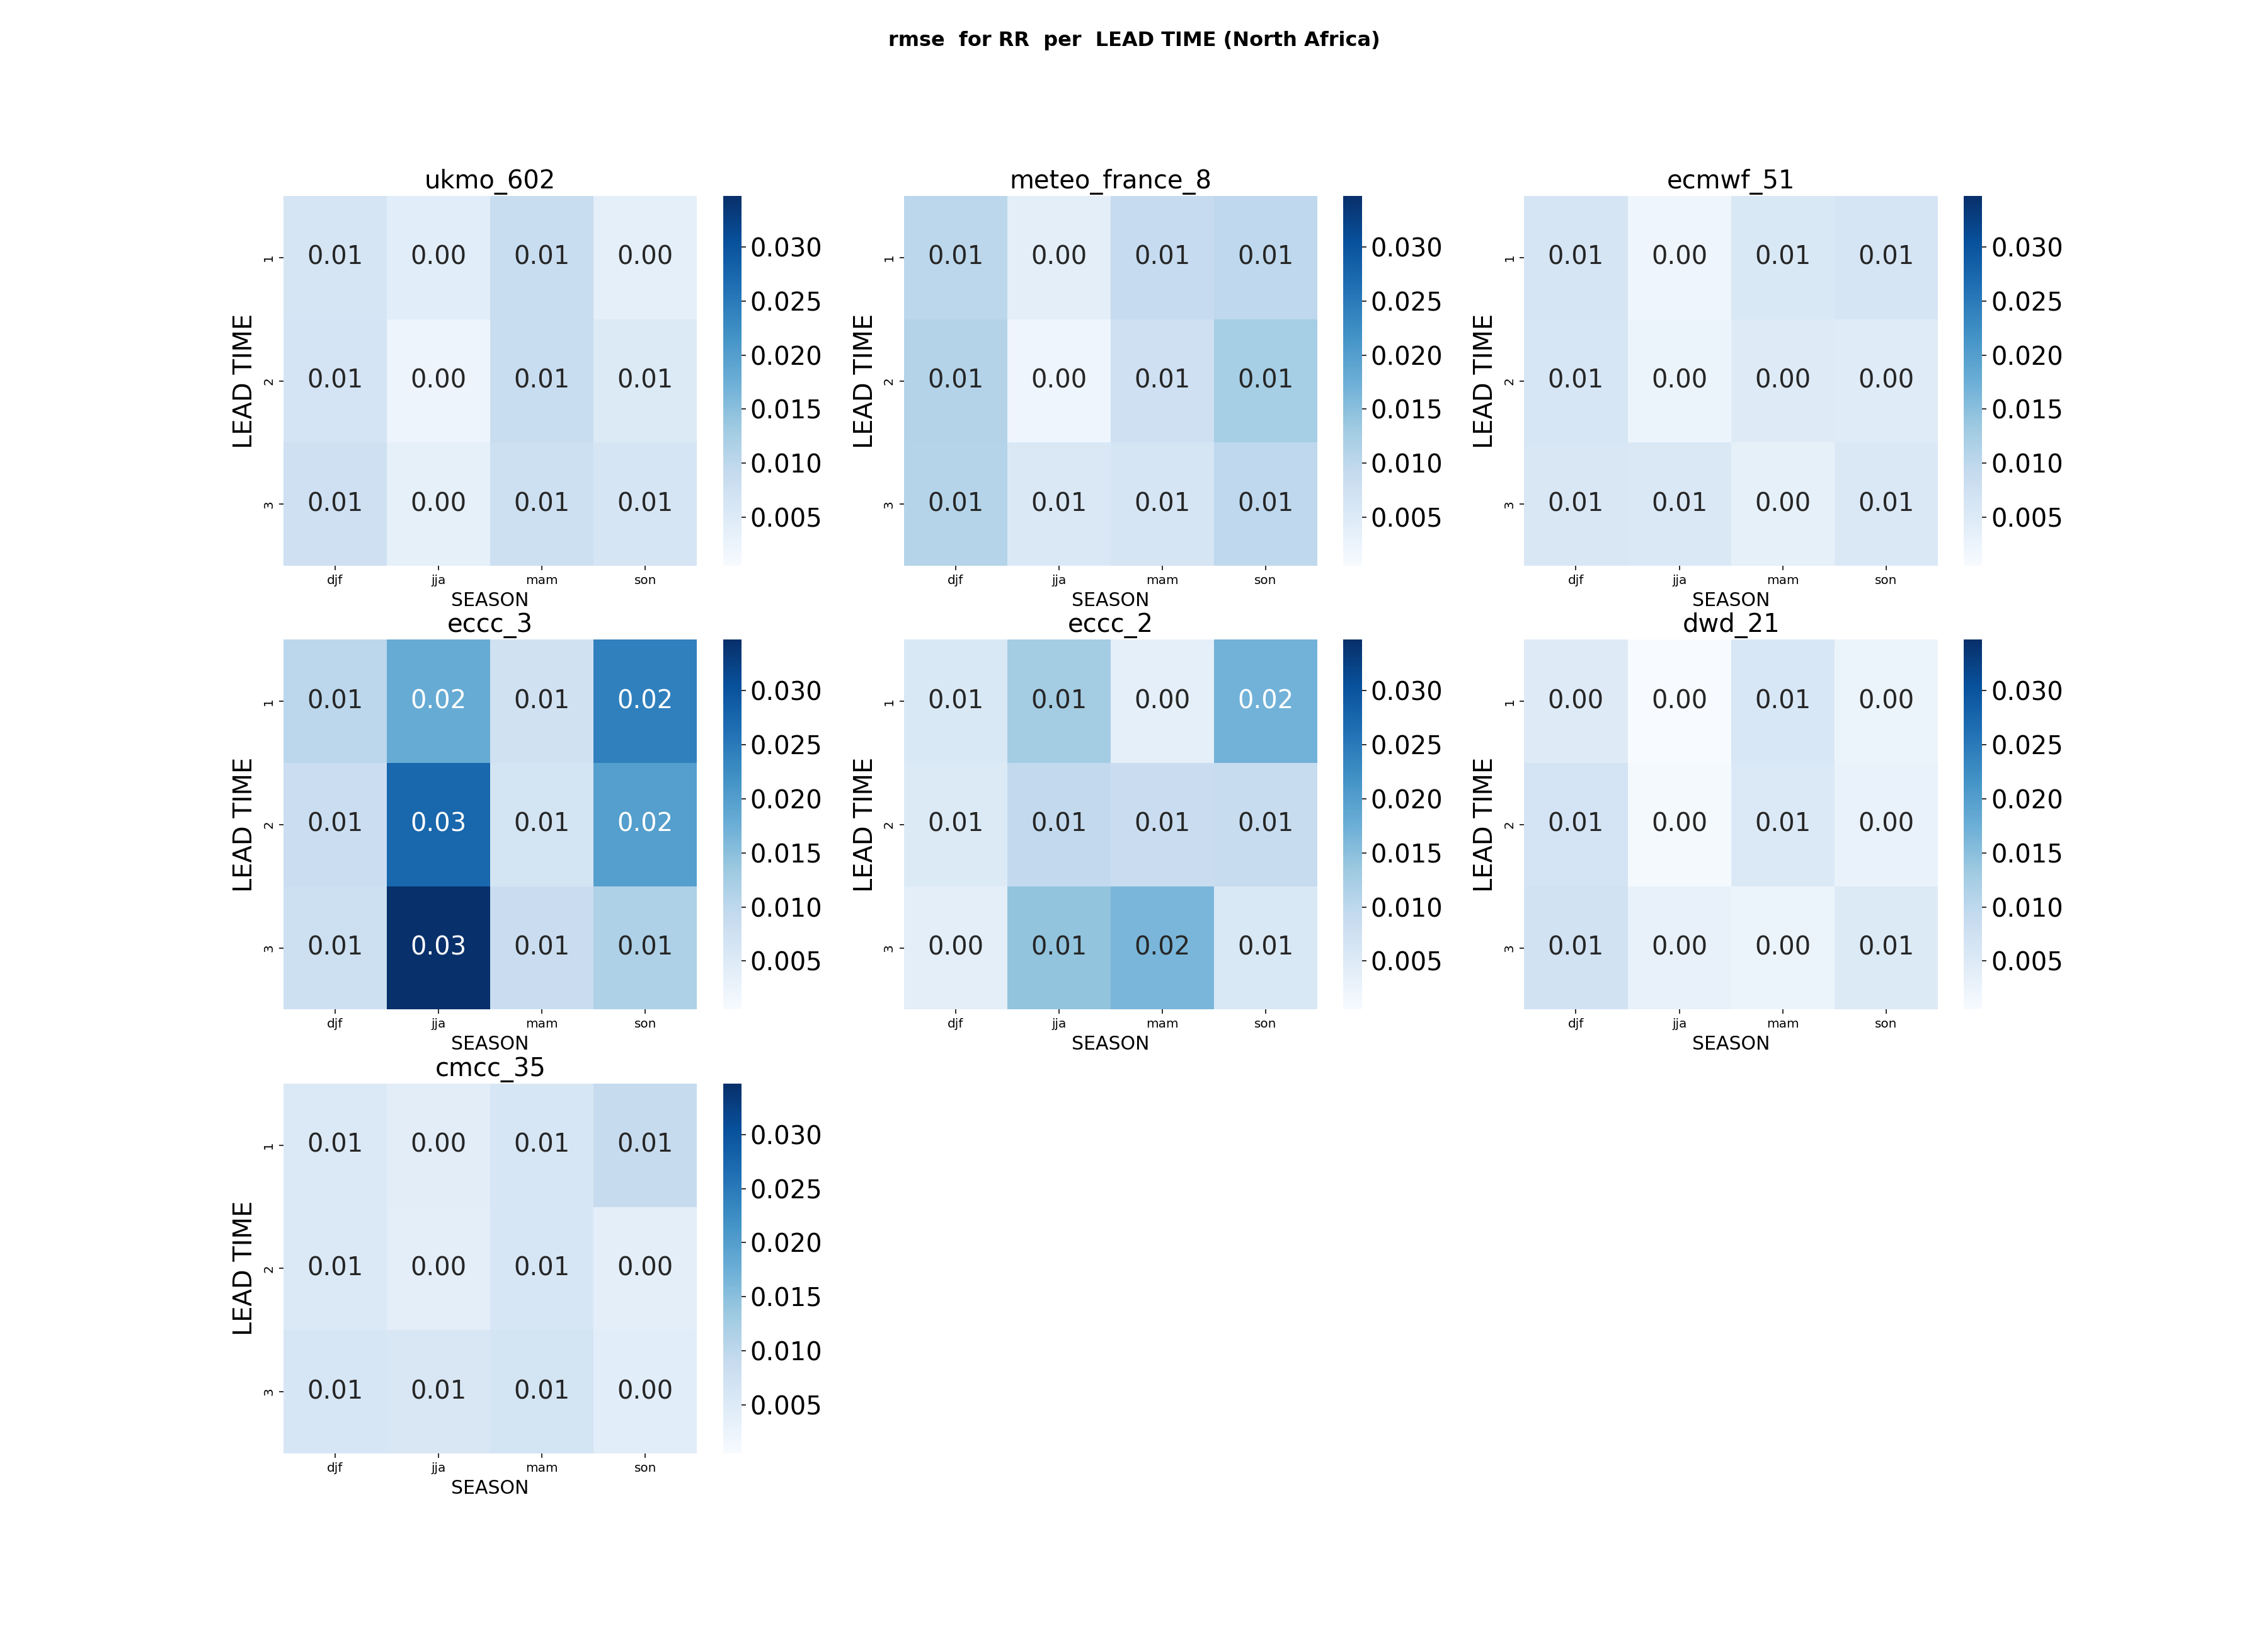
\includegraphics[scale=0.3]{plots/det/rmse/rmse_RR_NorthAfrica.png}
\caption{heatmap of RMSE For RR in mm (North Africa)}
\end{figure}

the RMSE is much better for North africa, the score is good over all lead-times and seasons. The centers, \textbf{\textit{ecmwf, ukmo and dwd}} show very good performance.

\vspace{1.5cm}
\paragraph{focus on Arabian Peninsula}:

\begin{figure}[H]
\centering
\includegraphics[scale=0.3]{plots/det/rmse/rmse_RR_ArabianPeninsula.png}
\caption{heatmap of RMSE For RR in mm (North Africa)}
\end{figure}

In the same way as North Africa, the RMSE for the Arabian Peninsula is much better than mena. The centers, \textbf{\textit{ecmwf, ukmo and dwd}} show very good performance.

\subsubsection{Analysis of Coefficient of Determination results}

\paragraph{focus on North Africa}

there is no big difference in North Africa.


\vspace{1.5cm}
\paragraph{focus on Arabian Peninsula}:


\begin{figure}[H]
\includegraphics[scale=0.3]{plots/det/rsquared/rsquared_RR_ArabianPeninsula.png}
\caption{Heatmap of RR  RSQUARED in MENA Region for all centers Arabian Peninsula}
\end{figure}

the R-SQUARED for the Arabian Peninsula shows a little improvement.

\subsection{Probabilistic Evaluation Metrics}

\subsubsection{Analysis of The Brier Score results}

\paragraph{focus on North Africa}:

there is no big difference in North Africa.
\vspace{1.5cm}
\paragraph{focus on Arabian Peninsula}:
there is no big difference in North Africa.

\subsubsection{ Analysis of Reliability results}
\paragraph{focus on North Africa}:

there is no big difference in North Africa.

\paragraph{focus on Arabian Peninsula}:


there is no big difference in North Africa.



\begin{figure}[H]
    \centering
    \includegraphics[scale=0.25]{plots/prob/rela/rela_RR_ArabianPeninsula.png}
    \caption{The Reliability Score ArabianPeninsula . \textbf{\textit{(0 means perfect Reliability )}}}
\end{figure}

There is a little Decline in the reliability of the Arabian Peninsula, especially f\textbf{\textit{ukmo}}

\subsubsection{Analysis of The ranked probability score results}
\paragraph{focus on north africa:}

there is no big difference in North Africa.

\paragraph{focus on Arabian Peninsula}:

there is no big difference on Arabian Peninsula.
\subsubsection{Analysis of Receiver Operating Characteristic results}
\paragraph{focus on north africa:}

there is no big difference in North Africa.
	
\paragraph{focus on Arabian Peninsula}:



\begin{figure}[H]
    \centering
    \includegraphics[scale=0.25]{plots/prob/roc/roc_RR_category_ArabianPeninsula.png}
    \caption{The ROC Score for each category Arabian Peninsula . \textbf{\textit{(1 means perfect ROC)}}}
\end{figure}


\begin{figure}[H]
    \centering
    \includegraphics[scale=0.25]{plots/prob/roc/roc_RR_lead_time_ArabianPeninsula.png}
    \caption{The average of  ROC Score on all categories for Arabian Peninsula . \textbf{\textit{(1 means perfect ROC)}}}
\end{figure}


For the roc score, the focus on Arabian Peninsula in category, show no big difference, as for the analysis along lead-time, there is a few improvement for DJF, MAM and SON, instead of JJA that shows low values for all centers. 													\subsubsection{Analysis of Relative operating characteristics Skill Score results }
\paragraph{focus on north africa:}
\begin{figure}[H]
    \centering
    \includegraphics[scale=0.25]{plots/prob/rocss/rocss_RR_category_NorthAfrica.png}
    \caption{The ROCSS Score for each category North Africa . \textbf{\textit{(1 means perfect ROCSS)}}}
\end{figure}


\begin{figure}[H]
    \centering
    \includegraphics[scale=0.25]{plots/prob/rocss/rocss_RR_lead_time_NorthAfrica.png}
    \caption{The average of  ROCSS Score on all categories    . \textbf{\textit{(1 means perfect ROCSS)}}}
\end{figure}


the rocss for North Africa is in general lower, thus the performance is less accurate.

\paragraph{focus on Arabian Peninsula}:
\begin{figure}[H]
    \centering
    \includegraphics[scale=0.25]{plots/prob/rocss/rocss_RR_lead_time_ArabianPeninsula.png}
    \caption{The average of  ROCSS Score on all categories for Arabian Peninsula . \textbf{\textit{(1 means perfect ROCSS)}}}
\end{figure}


the rocss for Arabian Peninsula is in general lower, thus the performance is less accurate.


 
\chapter{CONCLUSION}
This study has thoroughly evaluated the performance of leading climate models in predicting temperature and precipitation across the MENA region, North Africa, and the Arabian Peninsula. By assessing key metrics such as Accuracy (ACC), Root Mean Square Error (RMSE), Coefficient of Determination (R²), Brier Score (BS), ROC score, and others we have identified the strengths and weaknesses of each model, while highlighting regional variations in their predictive capabilities.

For temperature, all climate models demonstrated generally similar performance in the MENA region, with ECMWF consistently emerging as the most reliable model, achieving top performance in both deterministic and probabilistic metrics across all regions. However, in probabilistic metrics, UKMO showed comparatively lower performance than other models.

For precipitation, all models performed less effectively compared to their temperature predictions, particularly in the MENA region. ECMWF once again demonstrated the highest performance across all metrics and regions, showcasing its robustness in handling diverse climatic conditions. METEOFRANCE, CMCC, DWD, and UKMetOffice exhibited similar performance in deterministic measures such as ACC and RMSE. However, in probabilistic metrics, most models showed approximately similar performance, with UKMetOffice demonstrating comparatively lower performance, particularly in the Arabian Peninsula, where challenges related to the region’s hyper-arid climate and limited observational data are evident. 

It is worth noting that the models perform better for temperature predictions than for precipitation in the MENA region. This contrasts with tropical regions, where models tend to excel in both precipitation and temperature forecasting due to the more predictable influence of large-scale climate drivers such as ENSO. The limited observational data and complex climate dynamics in arid and semi-arid regions of MENA further challenge precipitation predictions, reducing model accuracy compared to temperature forecasts.

 In conclusion, climate models generally exhibit similar performance across the four classical seasons, with ECMWF consistently demonstrating higher performance compared to the other models. Each model provides valuable complementary strengths depending on the season and region. These findings highlight the importance of using multi-model ensembles to leverage the strengths of each model, improve seasonal forecast accuracy, and correct the influence of prominent modes of climate variability, such as ENSO and NAO, in the climate models using state-of-the-art statistical techniques.



%\begin{table}[h!]
%\centering
%\begin{tabular}{|>{\raggedright\arraybackslash}m{2cm}|>{\raggedright\arraybackslash}m{4cm}|>{\raggedright\arraybackslash}m{4cm}|>{\raggedright\arraybackslash}m{4cm}|}
%\hline
%\textbf{Metric} & \textbf{MENA} & \textbf{North Africa} & \textbf{Arabian Peninsula} \\ \hline
%ACC            & ECMWF, METEO-FRANCE, ECCC-3 & ECMWF, UKMO, ECCC-3 & ECMWF, UKMO, DWD \\ \hline
%RMSE           & UKMO, ECMWF & METEO-FRANCE & METEO-FRANCE \\ \hline
%R²             & ECMWF       & ECMWF         & ECMWF \\ \hline
%BS             & METEO-FRANCE, ECMWF, CMCC-35 & ECMWF, METEO-FRANCE, CMCC-35 & ECMWF, METEO-FRANCE, CMCC-35 \\ \hline
%RELA           & ALL except UKMO & ALL except UKMO & ALL except UKMO \\ \hline
%RPS            & ECMWF       & ECMWF         & ECMWF \\ \hline
%ROC            & ALL centers & ALL centers   & ALL centers \\ \hline
%ROCSS          & ALL centers & ALL centers   & ALL centers \\ \hline
%\end{tabular}
%\caption{Comparison of Metrics across MENA, North Africa, and Arabian Peninsula for TEMPERATURE.}
%\label{tab:temperature_metrics}
%\end{table}
%
%
%
%
%\begin{table}[h!]
%\centering
%\begin{tabular}{|>{\raggedright\arraybackslash}m{2cm}|>{\raggedright\arraybackslash}m{4cm}|>{\raggedright\arraybackslash}m{4cm}|>{\raggedright\arraybackslash}m{4cm}|}
%\hline
%\textbf{Metric} & \textbf{MENA} & \textbf{North Africa} & \textbf{Arabian Peninsula} \\ \hline
%ACC & ECMWF, CMCC-35, UKMO & ECMWF, UKMO and METEO-FRANCE & ECMWF, CMCC-35, UKMO \\ \hline
%RMSE & DWD, ECMWF and UKMO & ECMWF, UKMO and DWD & ECMWF, UKMO and DWD \\ \hline
%R² & ECMWF & ECMWF & CMCC-35, ECCC2 \\ \hline
%BS & ECMWF, METEO-FRANCE and CMCC-35 & ECMWF, METEO-FRANCE and CMCC-35 & ECMWF, METEO-FRANCE and CMCC-35 \\ \hline
%RPS & ALL except UKMO & ALL except UKMO & ALL except UKMO \\ \hline
%ROC & ALL & ALL & ALL \\ \hline
%ROCSS & ecmwf & ecmwf & ukmo, cmcc-35 \\ \hline
%RELA & ECMWF, CMCC and METEO-FRANCE & ECMWF, CMCC and METEO-FRANCE & METEO-FRANCE, DWD \\ \hline
%\end{tabular}
%\caption{Comparison of Metrics across MENA, North Africa, and Arabian Peninsula for PRECIPITATION}
%\label{tab:comparison}
%\end{table}
%%\chapter{Results}
\chapter{Results}
This chapter presents the results of our study, divided into two main sections: temperatures and precipitation. In each section, we provide a comprehensive analysis of the deterministic and probabilistic evaluation of forecast performance across the MENA region. By examining both temperature and precipitation metrics, we aim to highlight the strengths and limitations of the forecasting models, offering valuable insights into their reliability and applicability in this climatically diverse area.
%\section{Temperature}
%
%In the temperature session, the use of heatmaps and temperature metrics maps will allow for a visual interpretation of model performance across various metrics. By analyzing these heatmaps, we can identify the most effective models based on metrics such as Spearman rank correlation, RMSE (Root Mean Square Error), and the Coefficient of Determination (R²). These visualizations will help in understanding the relationships between predicted and observed temperatures, aiding in the selection of models with the highest predictive accuracy. Additionally, the use of probabilistic evaluation metrics such as the Brier Score, Reliability, Ranked Probability Score (RPS), and Relative Operating Characteristics (ROC) will provide insights into the model's performance in terms of forecast quality, focusing on calibration, discrimination, and sharpness. These methods will be used to refine and improve predictive models for temperature forecasting in the MENA region.
%\subsection{Deterministic evaluation results}
%\subsubsection{ACC}
%
%The provided images used in this section displays the correlation between observed and modeled surface temperatures across the MENA region for four different seasons: June, July, and August (JJA); December, January, February (DJF); March, April, May (MAM); and September, October, November (SON). Each map visualizes the predictive accuracy of various climate models, with the color intensity representing the strength and direction of the correlation between the models' predictions and the observed data. Hatched areas on the maps indicate regions where the correlation is statistically significant (p \(\leq\) 0.05). These maps are essential for evaluating the performance of climate models across different seasons and understanding which models provide the best temperature forecasts for the MENA region.
%\begin{figure}[H]
%    \centering
%    \includegraphics[width=1\linewidth]{plots/det/acc/ANOMALY_CORRELATION_djf_t2m.png}
%    \caption{Temperature correlation maps for DJF (December-January-February)}
%\end{figure}
%The analysis of the \textbf{Spearman rank correlation for djf } from the figures above shows the following trends:
%
%\begin{itemize}
%    \item For the \textbf{UKMO model}, the correlation between observed and modeled temperatures is high (around 0.7) in southeastern Libya, Egypt, and northwestern Sudan. However, it is low and negative in Morocco, Algeria, and parts of Libya.
%    \item The \textbf{Meteo-France model} exhibits a similar pattern, with high correlations in southeastern Libya and Egypt but low and negative values in Morocco and Algeria.
%    \item In contrast, the \textbf{ECMWF model} shows higher correlations in Saudi Arabia and Yemen.
%    \item For the \textbf{ECCC System 3 model}, the correlations are notably higher over a large part of the region, indicating better agreement between observed and modeled temperatures.
%\end{itemize}
%\begin{figure}[H]
%    \centering
%    \includegraphics[width=1\linewidth]{plots/det/corr/CORR_mam_t2m.png}
%    \caption{temperature correlation maps for mam}
%\end{figure}
%For MMA, the Met Office, ECMWF, and DWD demonstrate better performance across this region, except in northern Morocco, where correlations range between approximately -0.12 and 0.02.
%\begin{figure}[H]
%    \centering
%    \includegraphics[width=1\linewidth]{plots/det/corr/CORR_jja_t2m.png}
%    \caption{temperature correlation maps for jja}
%   
%\end{figure}
%For JJA, the ECMWF and ECCC-2 models exhibit the best correlations overall, except in southern Morocco and Tunisia, where their performance is notably weaker.
%\begin{figure}[H]
%    \centering
%    \includegraphics[width=1\linewidth]{plots/det/corr/CORR_son_t2m.png}
%    \caption{temperature correlation maps for son}
%   
%\end{figure}
%For SON , the Meteo-France model performs well, except in Egypt, showing better correlations in Morocco compared to other models and seasons. Similarly, the ECMWF model also performs well but shows weaker correlations in Libya and Egypt.
%\begin{figure}[H]
%    \centering
%    \includegraphics[width=1\linewidth]{plots/det/corr/corr_T2M_mena.png}
%    \caption{Temperature correlation heatmap for mena region}
%   
%\end{figure}
%
%
%The heatmaps provide an average overview of the models' performance across the MENA region for a given season and a forecast lead time ranging from 1 to 3 months. In general, correlations tend to decrease as the lead time increases from 1 to 3 months. For instance, the ECMWF model shows higher performance during JJA, whereas the ECCC-2 model performs better during MAM. As previously mentioned, these results represent averages over the entire region. For a more detailed analysis, a mask was applied to focus specifically on North African countries within the MENA region. The results of this targeted analysis are shown in the heatmap below.
%\begin{figure}[H]
%    \centering
%    \includegraphics[width=1\linewidth]{plots/det/corr/corr_T2M_NorthAfrica.png}
%    \caption{Temperature correlation heatmap for north africa}
%   
%\end{figure}
%\subsubsection{Root Mean Square Error}
%
%
%The maps in this section show the RMSE (Root Mean Square Error) between observed and modeled surface temperatures across the MENA region for the four seasons: JJA, DJF, MAM, and SON. The RMSE, expressed in the same units as temperature, evaluates the accuracy of climate models, with lower values indicating better performance.  These maps help identify the strengths and limitations of the models across seasons, contributing to the improvement of climate forecasts for the region.
%\begin{figure}[H]
%    \centering
%    \includegraphics[width=1\linewidth]{plots/det/rmse/rmse_T2M_mena.png}
%    \caption{Temperature rmse heatmaps for all the sasons}
%\end{figure}
%
%The heatmap for the seven models highlights distinct variations in their seasonal performance. The UKMO model shows moderate to good performance, particularly in JJA and MAM, as reflected by relatively low RMSE values ranging between 1.35°C and 1.51°C across the three lead times. This indicates that the UKMO model is reasonably effective in capturing surface temperature variations during these seasons, likely benefiting from its ability to simulate key atmospheric processes during these periods.
%
%In contrast, Météo-France exhibits weaker performance in JJA, with higher RMSE values suggesting less accurate predictions of surface temperatures during this season. This could be attributed to the model's limitations in capturing summer-specific temperature drivers in the MENA region, such as heatwaves, desert-air interactions, or seasonal atmospheric circulation patterns.
%
%The ECMWF model emerges as the best-performing model based on the heatmap, particularly during JJA, where it demonstrates high predictive accuracy and consistency. This is supported by the RMSE map, which shows significantly lower RMSE values across most of the MENA region. These low RMSE values confirm the ECMWF model's ability to capture regional temperature dynamics effectively, with reduced errors across diverse climatic zones.
%
%Notably, the spatial distribution of RMSE on the map reinforces the ECMWF's strong performance, as it maintains relatively low error values in critical parts of the MENA region. This suggests that the ECMWF model is better equipped to account for the complex climatic interactions in the region, such as the influence of desert regions, coastal temperature gradients, and seasonal weather patterns.
%
%Overall, these findings emphasize the importance of selecting climate models based on their seasonal and spatial performance, as they play a critical role in improving the accuracy of temperature forecasts for the MENA region.
%
%\begin{figure}[H]
%    \centering
%    \includegraphics[width=1\linewidth]{plots/det/rmse/rmse_jja_t2m.png}
%    \caption{temperature rmse maps for jja}
%\end{figure}
%To better understand the performance of climate models in sub-regions of MENA, a focus on North Africa is essential due to its distinct climatic features, such as vast desert landscapes, high seasonal temperature variability, and localized weather phenomena. The heatmap provides a comparative analysis of RMSE values for the seven models across this region, highlighting their seasonal accuracy in predicting surface temperatures.
%
%The North African climate, heavily influenced by the Sahara Desert and Mediterranean coast, presents unique challenges for climate modeling, such as accurately simulating extreme temperatures and their spatial distribution. By examining the heatmap, we can identify which models perform well in capturing these specific climatic patterns and assess their suitability for seasonal forecasting in this critical sub-region of MENA.
%\begin{figure}[H]
%    \centering
%    \includegraphics[width=1\linewidth]{plots/det/rmse/rmse_T2M_NorthAfrica.png}
%    \caption{Temperature rmse heatmap for north africa}
%   
%\end{figure}
%This specific analysis revealed that, although the ECMWF model performs well across the MENA region, its performance in North Africa is comparatively lower, except during JJA. As highlighted earlier, JJA remains the most accurate season for ECMWF in this sub-region, with RMSE values ranging between 1.34°C and 1.58°C. This indicates that the model effectively captures temperature dynamics in the summer, likely due to its ability to simulate key seasonal factors such as strong solar heating and atmospheric circulation patterns specific to North Africa during this period.
%
%In contrast, Météo-France demonstrates consistent performance across the three lead times and, on average, performs well over the four seasons in North Africa, particularly during SON. This could be attributed to the model’s ability to account for transitional weather conditions in autumn, such as changes in atmospheric pressure systems and coastal influences that significantly impact temperatures in this region.
%
%These observations underline the importance of analyzing sub-regional performance to identify models that are better suited for specific areas and seasons. While ECMWF excels in JJA, Météo-France shows a more balanced performance throughout the year, making it potentially more reliable for multi-seasonal forecasting in North Africa.
%
%
%
%
%
%\subsubsection{Coefficient of Determination (\( R^2 \))}
%The maps in this section show the R-SQUARED between observed and modeled surface temperatures across the MENA region for the four seasons: JJA, DJF, MAM, and SON. R-SQUARED is a statistical measure that indicates how well the model explains the variability in observed data, with values closer to 1 signifying better performance. These maps provide valuable insights into the predictive skill of the climate models, highlighting their ability to capture seasonal temperature patterns.
%
%\begin{figure}[H]
%    \centering
%    \includegraphics[width=1\linewidth]{plots/det/rsquared/rsquared_T2M_mena.png}
%    \caption{Temperature rsquared heatmaps for all the seasons}
%\end{figure}
%
%Based on this deterministic metric (R-SQUARED), the ECMWF model demonstrates superior performance for lead time 1 across all four seasons, particularly during MAM. In general, the portion of variance explained by the model decreases as the lead time increases. This indicates that while the model is highly effective at capturing seasonal variability of surface temperatures in the short term, its predictive skill diminishes over longer time horizons.
%
%The strong performance during MAM highlights the ECMWF ability to capture the complexities of spring, a season marked by transitional weather patterns in the MENA region. The high R-SQUARED values during this period suggest that the model accurately reflects observed temperature variability by effectively simulating key drivers such as the gradual warming trend, atmospheric circulation changes, and the interaction between desert and coastal dynamics.
%
%Such precision underscores the ECMWF model's reliability for short-term seasonal forecasting, particularly during periods of heightened climatic variability like MAM. However, the decreasing performance with increasing lead times suggests the need for careful interpretation of forecasts beyond lead time 1, as uncertainty increases with longer projections.
%
%\begin{figure}[H]
%    \centering
%    \includegraphics[width=1\linewidth]{plots/det/rsquared/rsquared_T2M_NorthAfrica.png}
%    \caption{Temperature rsquared heatmaps for all the seasons North Africa}
%\end{figure}
%A closer look at North Africa reveals that the ECMWF model performs best during JJA, with R-SQUARED values increasing as the lead time increases-contrary to the trend observed for the MENA region as a whole, where performance typically decreases with longer lead times. This suggests that the ECMWF model is particularly adept at capturing the persistent summer temperature patterns in North Africa, which may benefit from stronger model predictability over time due to the relatively stable atmospheric and climatic conditions during JJA.
%
%Similarly, Météo-France also shows good performance in North Africa, maintaining consistent R-SQUARED values across different lead times and seasons. This consistency highlights the model’s ability to handle the diverse climatic features of the region, such as the extreme temperatures influenced by the Sahara Desert and the moderating effects of the Mediterranean coastline.
%
%These findings emphasize the importance of regional analysis, as the performance of climate models can vary significantly within sub-regions of MENA. While ECMWF excels in predicting North Africa’s summer temperatures, the observed increase in R-SQUARED with lead time underscores the need to investigate the underlying factors driving this unusual trend, which contrasts with the broader MENA region's dynamics.
%
%
%
%
%\subsection{Probabilistic evaluation results}
%
%To complement the deterministic evaluation of model performance, probabilistic evaluation metrics are employed to assess the reliability and skill of climate models in predicting the likelihood of specific outcomes. Unlike deterministic metrics, which focus on the accuracy of single-point predictions, probabilistic metrics evaluate the quality of the models’ forecast distributions, accounting for uncertainty and variability in predictions. These metrics are essential for understanding how well models represent the range of possible outcomes, particularly in regions like MENA, where climatic variability and extremes are prominent. By incorporating probabilistic metrics, this analysis provides a more comprehensive evaluation of the models’ predictive capabilities and their usefulness in decision-making under uncertainty.
%The figures illustrate two main approaches to probabilistic assessment metrics, including the Brier Score (BS) and others. The first approach averages across lead times and grid points, while preserving categories, where the final figure contains the value of the metric for each season across all four seasons, for each category (mean, lower, upper) defined by the 1/3 quartiles. This method provides insight into the predictive ability of models under different seasonal conditions and forecast probability categories, particularly how well models capture temperature variations in the middle, lower, and upper quartiles of the predicted probability distribution. The diversity of metric values ​​across these categories helps highlight the sensitivity of models to different levels of forecast confidence. It indicates their ability to differentiate between forecast uncertainty and actual observed outcomes, providing a nuanced understanding of how accurately models predict different temperature ranges.
%
%The second approach averages all grid points in the MENA region while retaining all lead times and seasons. This aggregated view provides an overall assessment of the measure for each season, considering all lead times and forecast categories. This approach focuses on how models perform across different forecast scenarios and how well they produce accurate and reliable temperature forecasts, regardless of forecast probability. By retaining lead times and seasons in the analysis, this method provides a comprehensive picture of model performance over time and under different climate conditions. It reveals how well models generalize across different forecast scenarios, helping to identify which models are most effective at producing consistent and reliable forecasts.
%\subsubsection{Brier score}
%
%The figure at the bottom illustrates that most models demonstrate relatively high performance, as indicated by a small Brier Score (BS), meaning that the predicted probabilities are close to the observed ones. This reflects accurate forecast probabilities forT2M The UKMO model, however, shows moderate performance with a larger BS, suggesting that its predicted probabilities are less closely aligned with observed outcomes compared to other models. Notably, the middle category presents lower performance relative to the other two categories (lower and upper). This indicates that while some models capture temperature variability well in extreme conditions (upper category), their skill diminishes when forecasting moderate changes (middle category). This discrepancy highlights the challenges models face in translating predicted probabilities into reliable forecasts, particularly for temperature variations that are neither extreme nor outlier events. 
%
%
%\begin{figure}[H]
%    \centering
%    \includegraphics[width=1\linewidth]{plots/prob/bs/bs_T2M_category.png}
%    \caption{Temperature Brier score heatmaps for all the seasons per categories}
%\end{figure}
%An analysis by lead time revealed that the models Meteo France, ECMWF, and CMCC exhibit superior performance, as indicated by lower Brier Scores (BS). This suggests that these models provide more accurate probabilistic forecasts for T2M compared to others. Moreover, the differences in BS values between successive lead times are minimal, indicating that the predictive skill of these models remains relatively consistent as the forecast horizon increases.
%
%This stability in performance across lead times is particularly noteworthy, as it reflects the robustness of these models in maintaining their ability to produce reliable forecasts over time. The lower BS values also suggest that these models effectively capture the relationship between predicted probabilities and observed outcomes, ensuring high confidence in their probabilistic predictions. Such consistent performance across lead times is crucial for operational forecasting, as it highlights these models' reliability for both short- and medium-term forecasts in the MENA region.
%
%\begin{figure}[H]
%    \centering
%    \includegraphics[width=1\linewidth]{plots/prob/bs/bs_T2M_lead_time.png}
%    \caption{Temperature brier score heatmaps for all the seasons per lead time}
%\end{figure}
%o further evaluate the performance of these models and assess whether the same interpretations apply, the analysis will now focus specifically on the North African region. By examining the Brier Score metrics in this sub-region, we aim to determine whether the observed trends, such as the consistency of model performance across lead times and the relative strengths of ECMWF, CMCC, and Meteo France, remain valid or if different patterns emerge due to the unique climatic conditions and variability in North Africa.
%
%\begin{figure}[H]
%    \centering
%    \includegraphics[width=1\linewidth]{plots/prob/bs/bs_T2M_category_NorthAfrica.png}
%    \caption{Temperature Brier score heatmaps for all the seasons per categories for north africa}
%\end{figure}
%A closer analysis focused on the North African region revealed that the performance of the top-performing models—ECMWF, CMCC, and Meteo France—remains consistent. The zoomed evaluation shows that these models continue to exhibit low Brier Scores, indicating reliable probabilistic predictions across lead times. This finding suggests that the unique climatic conditions of North Africa do not significantly alter the predictive skill of these models, reaffirming their robustness and adaptability to sub-regional variations within the broader MENA context.
%
%
%\begin{figure}[H]
%    \centering
%    \includegraphics[width=1\linewidth]{plots/prob/bs/bs_T2M_lead_time_NorthAfrica.png}
%    \caption{Temperature brier score heatmaps for all the seasons per lead time North Africa}
%\end{figure}
%The results by lead time reveal similar conclusions, showing a consistent stability in Brier Scores across different lead times. This indicates that the predictive skill of the top-performing models, such as ECMWF, CMCC, and Meteo France, remains robust even as the forecast horizon increases. The minimal variation in scores across lead times underscores the reliability of these models for producing accurate probabilistic forecasts, regardless of the temporal range considered.
%\subsubsection{Reliability}
%The reliability diagrams presented for the season assess the probabilistic performance of the seven climate models across three forecast categories: lower tercile , middle tercile , and upper tercile . These diagrams compare the predicted forecast probabilities to the observed frequencies, providing a clear indication of the models' ability to produce reliable temperature forecasts. A perfectly reliable model would align closely with the diagonal, where predicted probabilities match observed outcomes. By analyzing these diagrams, we can identify which models perform best for specific categories and uncover any systematic biases, such as over- or under-forecasting certain probabilities. This evaluation is crucial for understanding the strengths and weaknesses of the models, particularly in their ability to capture temperature extremes and moderate conditions .
%
%
%\begin{figure}[H]
%    \centering
%    \includegraphics[width=1\linewidth]{plots/prob/rela/rela_diagram_t2m_djf.png}
%    \caption{temperature reliabilty maps for djf}
%\end{figure}
%
%For the DJF season, the reliability diagrams show that most models exhibit similar performance, with the exception of UKMO, which significantly overestimates probabilities across all categories. For ECMWF, there is a noticeable overestimation in the upper tercile (warm extremes) starting at a forecast probability of approximately 0.6, indicating that the model tends to assign higher probabilities to warm events compared to their observed frequencies. Conversely, ECMWF shows a systematic underestimation for both the lower and middle terciles across most probabilities. For the remaining models, except UKMO, there is a general trend of underestimation across all three categories, beginning at forecast probabilities around 0.5. This pattern suggests that while the models capture some aspects of the observed temperature distribution, they struggle to provide accurate probabilities for more extreme or moderate conditions, especially at higher forecast probabilities. These results highlight the challenges faced by the models in reliably predicting temperature outcomes during the winter season (DJF), particularly for extreme categories.
%For the other three seasons (JJA, MAM, and SON), the reliability diagrams reveal a general tendency for most models to underestimate probabilities across all tercile categories, starting at approximately 0.4. This underestimation indicates that the models tend to be over-cautious, predicting lower probabilities than what is observed in reality. However, UKMO still stands out as an exception, showing a consistent overestimation across the forecast range, particularly for higher probabilities. This suggests that UKMO tends to assign excessively high probabilities to events that occur less frequently than predicted, which reduces its reliability. Overall, this recurring underestimation in the majority of models highlights their difficulty in accurately capturing the likelihood of temperature outcomes, especially beyond moderate probabilities. 
%
%\begin{figure}[H]
%    \centering
%    \includegraphics[width=1\linewidth]{plots/prob/rela/rela_T2M_mena.png}
%    \caption{temperature reliabilty heatmap}
%\end{figure}
%The heatmap further confirms the analyses derived from the reliability diagrams. It highlights similar trends observed across the models and seasons.Conversely, UKMO continues to stand out with its consistent overestimation of probabilities, aligning with the overconfidence seen in the reliability diagrams. This agreement between the heatmap and the reliability curves strengthens confidence in the identified patterns .
%\begin{figure}[H]
%    \centering
%    \includegraphics[width=1\linewidth]{plots/prob/rela/rela_T2M_NorthAfrica.png}
%    \caption{temperature reliabilty heatmap for north africa}
%\end{figure}
%
%A more focused analysis on North Africa has not significantly altered the overall conclusions derived from the broader MENA region. The consistent performance patterns observed across the different models and seasons remain largely unchanged when examining the North African context. 
%
%
%
%
%\subsubsection{The ranked probability score }
%
%The Ranked Probability Score (RPS) provides a valuable measure of forecast performance by evaluating the accuracy of probabilistic predictions across different categories. It combines both the skill in predicting the occurrence of events and the sharpness of the forecast distribution. By comparing the forecasted probability distribution against the observed outcomes, the RPS quantifies the deviation between the predicted and actual probabilities. A lower RPS value indicates better forecast accuracy, reflecting both how well the forecast aligns with observed frequencies and how well it discriminates between different probability categories. This metric helps to identify which models offer the most reliable probabilistic predictions, particularly in terms of capturing the likelihood of various temperature outcomes within a given forecast period.
%\begin{figure}[H]
%    \centering
%    \includegraphics[width=1\linewidth]{plots/prob/rps/rps_T2M_mena.png}
%    \caption{Temperature RPS  heatmaps for all the seasons per categories}
%\end{figure}
%The figure displaying the Ranked Probability Score (RPS) for different climate models and seasonal periods provides a detailed view of model performance across various start months (DJF, JJA, MAM, SON). Each cell in the matrix represents the RPS value for a specific model and season combination, with the color intensity indicating how well the forecast probabilities match the observed data.
%
%From this figure, it is evident that ECMWF consistently shows lower RPS values, indicating better predictive accuracy across different seasons. This suggests that ECMWF's forecasts are more closely aligned with observed temperature variability. The relatively higher RPS values for  UKMO model underscore their challenges in accurately capturing temperature variations. 
%For the North African region, the results mirror those observed in the broader MENA region.  
%
%This suggests that despite the localized focus on North Africa, the model performance differences remain significant, particularly for UKMO. 
%
%
%
%\begin{figure}[H]
%    \centering
%    \includegraphics[width=1\linewidth]{plots/prob/rps/rps_T2M_NorthAfrica.png}
%    \caption{Temperature RPS  heatmaps for north africa}
%\end{figure}
%\subsubsection{Receiver Operating Characteristic}
%The ROC (Receiver Operating Characteristic) curve is an important tool for evaluating the performance of predictive models, particularly in the context of probabilistic forecasts. It provides a graphical representation of the trade-off between the true positive rate  and the false positive rate  across various threshold levels.
%
%\begin{figure}[H]
%    \centering
%    \includegraphics[width=1\linewidth]{plots/prob/roc/roc_T2M_category.png}
%    \caption{Temperature AUC  heatmaps }
%\end{figure}
%
%
%Models generally exhibit similar performance, as indicated by the high Area Under the ROC Curve (AUC) values, which reflect their ability to effectively discriminate between predicted probabilities and observed outcomes. Unlike the reliability metric, where UKMO showed weaker performance, it performs relatively well in terms of the AUC, demonstrating good skill in distinguishing between forecasted events and non-events. Similar to the findings with the Brier Score (BS), the "middle" probability category tends to show weaker performance compared to the "lower" and "upper" categories. This highlights the models' greater sensitivity in accurately predicting events with extreme probabilities (high or low), but reduced skill for moderate probability scenarios. This consistency across metrics underscores the need to address forecast performance specifically in the middle category to further improve model predictions.
%
%\begin{figure}[H]
%    \centering
%    \includegraphics[width=1\linewidth]{plots/prob/roc/roc_T2M_category_NorthAfrica.png}
%    \caption{Temperature AUC  heatmaps for north africa }
%\end{figure}
%The figure above confirms the same conclusions for the North Africa region. The models generally maintain similar performance, with high AUC values reflecting strong discrimination skill across all categories. UKMO continues to show robust results in terms of ROC, despite its weaker reliability performance. As observed previously, the "middle" probability category remains the least performant compared to the "lower" and "upper" categories, indicating the models' reduced ability to predict moderate probability events. This consistency in findings suggests that the regional focus on North Africa does not significantly alter the overall assessment of model performance.
%\subsubsection{Relative operating characteristics Skill Score}
%ROCSS provides an assessment of a model's ability to discriminate between observed and forecasted events relative to a reference model, often a climatological or random forecast. A higher ROCSS indicates that the model has skill in distinguishing between occurrences and non-occurrences of an event, while a score close to zero suggests no significant improvement over the reference
%
%\begin{figure}[H]
%    \centering
%    \includegraphics[width=1\linewidth]{plots/prob/rocss/rocss_T2M_category.png}
%    \caption{Temperature ROCSS  heatmaps for MENA region }
%\end{figure}. 
%The ROC Skill Score (ROCSS) analysis reveals similar conclusions to the ROC results for Mena region and north Africa. The models generally demonstrate consistent and positive skill, highlighting their ability to discriminate between observed and forecasted events. UKMO, which showed weaker performance in reliability metrics, continues to perform well in terms of ROCSS, confirming its relative robustness in event discrimination. Additionally, as observed with the ROC scores, the "middle" category exhibits lower performance compared to the "lower" and "upper" categories. This indicates that while the models excel at predicting extreme events with high or low probabilities, their ability to capture moderate probability events remains limited.
%
%\begin{figure}[H]
%    \centering
%    \includegraphics[width=1\linewidth]{plots/prob/roc/roc_T2M_category_NorthAfrica.png}
%    \caption{Temperature ROCSS  heatmaps for north africa }
%\end{figure}
%
%




\section{PRECIPITATIONS}
IN general, the forecast of precipitations is more complicated than temperature, thus the scores are a little less good for this part especially the deterministic ones. 
\subsection{Deterministic Evaluation Metrics}

\subsubsection{ACC}

\begin{figure}[H]
	\centering
	\includegraphics[scale=0.25]{plots/det/acc/acc_RR_mena.png}
	\caption{The Heatmap of acc for the mena region for every period \textbf{\textit{(1 for perfect Correlation)} }}
\end{figure}
The acc is moderate for all centers; however, the best models are \textbf{\textit{ECMWF, UKMO, and CMCC-35}}. There is no clear variability in performance along lead-time. For SON, the performance is good at lead-time 2 for all centers. As for the other seasons, the performance is generally strong at the 1st lead-time but decreases with increasing lead-time.
Hence, Meteo-France also shows good performance, but it decreases significantly over time.



\begin{figure}[H]
\centering
\includegraphics[scale=0.3]{plots/det/acc/ANOMALY_CORRELATION_son_RR.png}
\caption{3-months Rolling mean of Anomaly Correlation in MENA Region for all centers SON}
\end{figure}
For temperature, the models demonstrate the best performance in the tropical regions. However, for precipitation, the situation is different. Hence the results show good performance during SON, where the Arabian Peninsula and  East Africa exhibit the highest performance.
\begin{figure}[H]
\centering
\includegraphics[scale=0.3]{plots/det/acc/ANOMALY_CORRELATION_djf_RR.png}
\caption{3-months Rolling mean of Anomaly Correlation in MENA Region for all centers DJF}
\end{figure}

The 3-month rolling mean for DJF acc shows that the best models are \textbf{\textit{ECMWF, UKMO, and Meteo-France}}. The acc is significant across most of the MENA region, except in the east of Africa. Thus, for all centers the East of Africa have the highest score. However, the \textbf{\textit{ecmwf and ukmo}} show good performance for 
the Arabian Peninsula. As for North Africa, theb\textbf{\textit{meteo-france}} shows good acc.

 
For SON, the situation is generally better than for DJF in the Arabian peninsula. In general, \textbf{\textit{ECMWF and Meteo-France}} are the best. Nevertheless, the correlation isn't significant in the east of africa and the north of the Arabian peninsula despite of the high acc.

\vspace{1.5cm}

\textbf{focus on north africa:}
according to the heatmap below, the correlation shows no big difference for the first lead-time, but for the second and third lead-times, it became lower. Thus, the \textbf{\textit{ecmwf,ukmo and meteo-france}} maintain relatively good correlation.


\begin{figure}[H]
	\centering
	\includegraphics[scale=0.25]{plots/det/acc/acc_RR_NorthAfrica.png}
	\caption{The Heatmap of ACC for the North Africa region for every period \textbf{\textit{(1 for perfect Correlation)} }}
\end{figure}

\vspace{1.5cm}
\textbf{focus on Arabian Peninsula}:

\begin{figure}[H]
	\centering
	\includegraphics[scale=0.25]{plots/det/acc/acc_RR_ArabianPeninsula.png}
	\caption{The Heatmap of acc for the mena region for every period \textbf{\textit{(1 for perfect Correlation)} }}
\end{figure}

The analysis of the Arabian Peninsula shows that the score is much better than the general situation of the mena region. The acc is good especially for SON for the second and third lead-times.

\subsubsection{RMSE}
 
for the Root Mean Squared Error, the best models shown in the heatmap below are \textbf{\textit{DWD, ECMWF and UKMO}}. The RMSE score demonstrate a moderate performance for all models especially \textbf{\textit{DWD, ECMWF and UKMO}}. The performance is stable over lead-times and it is much better for djf in all centers.

\begin{figure}[H]
\centering
\includegraphics[scale=0.3]{plots/det/rmse/rmse_djf_RR.png}
\caption{3-months Rolling mean of RMSE in MENA Region for all centers DJF in mm}
\end{figure}

\begin{figure}[H]
\centering
\includegraphics[scale=0.3]{plots/det/rmse/rmse_jja_RR.png}
\caption{3-months Rolling mean of RMSE in MENA Region for all centers JJA in mm}
\end{figure}

also for the spacial dimension, the RMSE stay stable and exhibit moderate performance for all centers. Thus, all models have almost the same skill and they are consistent with each other.

\begin{figure}[H]
\centering
\includegraphics[scale=0.3]{plots/det/rmse/rmse_RR_mena.png}
\caption{heatmap of RMSE For RR in mm}
\end{figure}

\vspace{1.5cm}

\textbf{focus on North Africa} : 
\begin{figure}[H]
\centering
\includegraphics[scale=0.3]{plots/det/rmse/rmse_RR_NorthAfrica.png}
\caption{heatmap of RMSE For RR in mm (North Africa)}
\end{figure}

the RMSE is much better for North africa, the score is good over all lead-times and seasons. The centers, \textbf{\textit{ecmwf, ukmo and dwd}} show very good performance.

\vspace{1.5cm}
\textbf{focus on Arabian Peninsula}:

\begin{figure}[H]
\centering
\includegraphics[scale=0.3]{plots/det/rmse/rmse_RR_ArabianPeninsula.png}
\caption{heatmap of RMSE For RR in mm (North Africa)}
\end{figure}

In the same way as North Africa, the RMSE for the Arabian Peninsula is much better than mena. The centers, \textbf{\textit{ecmwf, ukmo and dwd}} show very good performance.


\subsubsection{Coefficient of Determination (\( R^2 \))}
for precipitation, the R-SQUARED is very low, the maximum value is less than 0.1. However, the ecmwf is the best in term of R-SQUARED. for DJF,JJA and MAM the highest performance is in the first Lead-time, and it decrease along time, But for SON the best score is in the second Lead-time for all centers.
\begin{figure}[H]
	\centering
	\includegraphics[scale=0.25]{plots/det/rsquared/rsquared_RR_mena.png}
	\caption{The Heatmap of rsquared for Precipitations in the mena region for every period \textbf{\textit{(1 for perfect RSQUARED)} }}
\end{figure}


\begin{figure}[H]
\includegraphics[scale=0.3]{plots/det/rsquared/rsquared_son_RR.png}
\caption{3-months Rolling mean of RSQUARED in MENA Region for all centers SON}
\end{figure}

there is some isolated zones where the r-squared is good especially in Syria, Irak, Jordan ,Palestine  and East Africa, this high performance is observed in all centers. For the rest of the MENA region the performance is very bad with score near to 0. Hence, there is no constant pattern for the R-SQUARED, the spacial variation is very high for all centers.

\vspace{1.5cm}
\textbf{focus on North Africa}

there is no big difference in North Africa.


\vspace{1.5cm}
\textbf{focus on Arabian Peninsula}:


\begin{figure}[H]
\includegraphics[scale=0.3]{plots/det/rsquared/rsquared_RR_ArabianPeninsula.png}
\caption{Heatmap of RR  RSQUARED in MENA Region for all centers Arabian Peninsula}
\end{figure}

the R-SQUARED for the Arabian Peninsula shows a little improvement.


\subsection{Probabilistic Evaluation Metrics}

\subsubsection{The Brier Score (BS)}

\begin{figure}[H]
    \centering
    \includegraphics[scale=0.25]{plots/prob/bs/bs_RR_category.png}
    \caption{The Heatmap of Brier Score for each category  . \textbf{\textit{(0 represents perfect BS)}}}
\end{figure}

for the analysis per category, we can see in the figure above that all centers exhibit good performance in term of Brier Score except the UMKO that shows moderate BS. Overall, the middle tercile shows lower performance (higher Brier Score) for all centers. 
the figure below shows the analysis per lead-time. the same result is found, but the \textbf{\textit{ECMWF,METEO-FRANCE and CMCC-35}} are the best models in Brier Score for lead-time analysis.The performance stay stable along time which is a reliable signal. Despite the UKMO have the lower performance, it stays close to the other centers, the difference isn't so wide. 
In general, the performance stays stable over category, lead-time and space.


\begin{figure}[H]
    \centering
    \includegraphics[scale=0.25]{plots/prob/bs/bs_RR_lead_time.png}
    \caption{The Heatmap of Brier Score for lead-time. \textbf{\textit{(0 represents perfect BS)}}}
\end{figure}


\begin{figure}[H]
\includegraphics[scale=0.3]{plots/prob/bs/bs_mam_RR_middle.png}
\caption{3-months Rolling mean of Brier Score in MENA Region for all centers middle tercile MAM}
\end{figure}

the spacial distribution of the BS is homogeneous, the same performance across the MENA region, almost all centers perform well for all lead-times, for  tercile there is a little lower performance for the middle tercile.
Hint, for the other seasons the results are almost the same. 

\vspace{1.5cm}
\textbf{focus on North Africa}:

there is no big difference in North Africa.
\vspace{1.5cm}
\textbf{focus on Arabian Peninsula}:
there is no big difference in North Africa.

\subsubsection{Reliability}

\begin{figure}[H]
    \centering
    \includegraphics[scale=0.25]{plots/prob/rela/rela_RR_mena.png}
    \caption{The Reliability Score  . \textbf{\textit{(0 means perfect Reliability)}}}
\end{figure}

In the figure above, all centers demonstrate similar moderate performance in term of reliability. But deep analysis within the figure below, shows that UKMO has very bad performance, also we can distinguish three models that have the best reliability according to the reliability diagram, the centers are \textbf{\textit{ECMWF,CMCC and METEO-FRANCE}}. Hence,all centers give similar description of the reliability, also the stability along lead-time is a good indicator despite of the moderate results (0.3), we can rely on the models cited above because of the acceptable results and the stability along time.

\begin{figure}[H]
\centering
\includegraphics[scale=0.3]{plots/prob/rela/rela_diagram_RR_djf.png}
\caption{The 3-month rolling mean for Reliability DJF   . \textbf{\textit{Reliability is better in cases where the graphs are closer to the 45-degree line}}}
\end{figure}

for the reliability diagram, all centers show moderate results, except for the ukmo that shows lower reliability.Thus, for the lower and upper terciles, models in general show good reliability, but for the middle tercile, this models aren't reliable. above all, \textbf{\textit{ecmwf}}  shows the highest performance for reliability.

\vspace{1.5cm}
\textbf{focus on North Africa}:

there is no big difference in North Africa.

\vspace{1.5cm}
\textbf{focus on Arabian Peninsula}:

\begin{figure}[H]
    \centering
    \includegraphics[scale=0.25]{plots/prob/rela/rela_RR_ArabianPeninsula.png}
    \caption{The Reliability Score ArabianPeninsula . \textbf{\textit{(0 means perfect Reliability )}}}
\end{figure}

There is a little Decline in the reliability of the Arabian Peninsula, especially f\textbf{\textit{ukmo}}


\subsubsection{The ranked probability score (RPS)}


\begin{figure}[H]
    \centering
    \includegraphics[scale=0.25]{plots/prob/rps/rps_RR_mena.png}
    \caption{The Heatmap of  RPS Score on MENA region for Precipitations    . \textbf{\textit{(0 means perfect RPS)}}}
\end{figure}

In the figure above, all centers demonstrate moderate performance, except for UKMO, which shows noticeably lower performance. 


\begin{figure}[H]
    \centering
    \includegraphics[scale=0.25]{plots/prob/rps/rps_djf_RR.png}
    \caption{The   RPS Score on MENA region for Precipitations DJF   . \textbf{\textit{(0 means perfect RPS)}}}
\end{figure}

the spacial distribution of the RPS, is homogeneous, in all the region the score is good for all centers.Thus, the ukmo shows lower performance for this score.

\vspace{1.5cm}
\textbf{focus on North Africa}:

there is no big difference in North Africa.

\vspace{1.5cm}
\textbf{focus on Arabian Peninsula}:

there is no big difference in North Africa.


\subsubsection{Relative operating characteristics}

\begin{figure}[H]
    \centering
    \includegraphics[scale=0.25]{plots/prob/roc/roc_RR_category.png}
    \caption{The Heatmap of ROC Score for each category  . \textbf{\textit{(1 means perfect ROC)}}}
\end{figure}

In the figure above, it is evident that all centers exhibit similar performance levels. However, the middle tercile consistently achieves the lowest score.
\begin{figure}[H]
    \centering
    \includegraphics[scale=0.25]{plots/prob/roc/roc_RR_lead_time.png}
    \caption{The Heatmap of ROC Score for lead-times. \textbf{\textit{(1 means perfect ROC)}}}
\end{figure}

for the ROC score, all centers show similar good performance, in general the best score is observed for tha first lead-time, except for the SON season where the best performance is for the second lead-time.

\begin{figure}[H]
    \centering
    \includegraphics[scale=0.3]{plots/prob/roc/roc_son_RR_upper.png}
    \caption{The ROC Score Upper tercile SON    . \textbf{\textit{(1 means perfect ROC)}}}
\end{figure}

the spacial distribution of the roc score confirms an important result. For precipitation all centers shows better performance for the East of Africa, Irak,Syria,Jordan and Palestine. The performance in this zone is very high (score near to 1). For the rest of MENA region the performance is similar, with moderate to good score.

\vspace{1.5cm}
\textbf{focus on North Africa}:

there is no big difference in North Africa.


\vspace{1.5cm}
\textbf{focus on Arabian Peninsula}:

\begin{figure}[H]
    \centering
    \includegraphics[scale=0.25]{plots/prob/roc/roc_RR_category_ArabianPeninsula.png}
    \caption{The ROC Score for each category Arabian Peninsula . \textbf{\textit{(1 means perfect ROC)}}}
\end{figure}


\begin{figure}[H]
    \centering
    \includegraphics[scale=0.25]{plots/prob/roc/roc_RR_lead_time_ArabianPeninsula.png}
    \caption{The average of  ROC Score on all categories for Arabian Peninsula . \textbf{\textit{(1 means perfect ROC)}}}
\end{figure}


For the roc score, the focus on Arabian Peninsula in category, show no big difference, as for the analysis along lead-time, there is a few improvement for DJF, MAM and SON, instead of JJA that shows low values for all centers. 																																																					
\subsubsection{Relative operating characteristics Skill Score}

In the figure above, the ECMWF exhibit the best performance for all terciles and periods. However, we should notice that the performance is very low for the middle tercile in all centers. For the analysis along time, the performance is so low, the best performance is in the first lead-time, except the SON which shows the best performance for the second lead-time. Above all, the \textbf{\textit{ecmwf}} shows the best performance.

\begin{figure}[H]
    \centering
    \includegraphics[scale=0.25]{plots/prob/rocss/rocss_RR_category.png}
    \caption{The ROCSS Score for each category  . \textbf{\textit{(1 means perfect ROCSS)}}}
\end{figure}


\begin{figure}[H]
    \centering
    \includegraphics[scale=0.25]{plots/prob/rocss/rocss_RR_lead_time.png}
    \caption{The average of  ROCSS Score on all categories    . \textbf{\textit{(1 means perfect ROCSS)}}}
\end{figure}



\begin{figure}[H]
    \centering
    \includegraphics[scale=0.3]{plots/prob/rocss/rocss_mam_RR_upper.png}
    \caption{The ROC Skill Score Upper tercile MAM    . \textbf{\textit{(1 means perfect ROCSS)}}}
\end{figure}

the spacial distribution of the ROCSS, shows that all centers are consistent for this score. The spacial distribution isn't clear, there is a high spacial variability.

\vspace{1.5cm}
\textbf{focus on North Africa}:

\begin{figure}[H]
    \centering
    \includegraphics[scale=0.25]{plots/prob/rocss/rocss_RR_category_NorthAfrica.png}
    \caption{The ROCSS Score for each category North Africa . \textbf{\textit{(1 means perfect ROCSS)}}}
\end{figure}


\begin{figure}[H]
    \centering
    \includegraphics[scale=0.25]{plots/prob/rocss/rocss_RR_lead_time_NorthAfrica.png}
    \caption{The average of  ROCSS Score on all categories    . \textbf{\textit{(1 means perfect ROCSS)}}}
\end{figure}


the rocss for North Africa is in general lower, thus the performance is less accurate.

\vspace{1.5cm}
\textbf{focus on Arabian Peninsula}:

\begin{figure}[H]
    \centering
    \includegraphics[scale=0.25]{plots/prob/rocss/rocss_RR_category_ArabianPeninsula.png}
    \caption{The ROCSS Score for each category Arabian Peninsula . \textbf{\textit{(1 means perfect ROCSS)}}}
\end{figure}


\begin{figure}[H]
    \centering
    \includegraphics[scale=0.25]{plots/prob/rocss/rocss_RR_lead_time_ArabianPeninsula.png}
    \caption{The average of  ROCSS Score on all categories for Arabian Peninsula . \textbf{\textit{(1 means perfect ROCSS)}}}
\end{figure}


the rocss for Arabian Peninsula is in general lower, thus the performance is less accurate.


\subsubsection{summary}
\begin{table}[h!]
\centering
\begin{tabularx}{\textwidth}{@{}p{2.5cm}p{4cm}p{4cm}p{2.5cm}p{3cm}@{}}
\toprule
\textbf{Metric}       & \textbf{Focus}                                    & \textbf{What it Measures}                         & \textbf{Dependent on Observed Outcomes?} & \textbf{Visualization/Tools}             \\ \midrule
\textbf{Reliability}   & Probabilities match observed frequencies          & Calibration of probabilities                      & Yes                                      & Reliability diagram                      \\
\textbf{Discrimination} & Differentiating between outcomes                 & Ability to distinguish events from non-events    & Yes                                      & ROC curve, AUC                           \\
\textbf{Sharpness}     & Boldness of probabilities (away from average)     & Confidence of the forecast                        & No                                       & Histogram of forecast probabilities      \\
\textbf{Resolution}    & Informativeness and variability of forecast       & Ability to provide specific, useful info         & Yes                                      & Brier Score decomposition                \\ \bottomrule
\end{tabularx}
\caption{Key differences between reliability, discrimination, sharpness, and resolution in seasonal forecasting.}
\label{tab:forecast_metrics}
\end{table}

\newpage
\thispagestyle{empty}
\mbox{}

\endinput


%\chapter{FOCUS ON NORTH AFRICA}

\section{Temperature}

\subsection{Deterministic evaluation results}
\subsubsection{\textbf{Correlation}}


\begin{figure}[H]
    \centering
    \includegraphics[width=1\linewidth]{plots/det/corr/corr_T2M_NorthAfrica.png}
    \caption{Temperature heatmap for north africa}
   
    \label{CORR_mam_t2m.png}
\end{figure}
\subsubsection{Root Mean Square Error}



\begin{figure}[H]
    \centering
    \includegraphics[width=1\linewidth]{plots/det/rmse/rmse_T2M_NorthAfrica.png}
    \caption{Temperature heatmap for north africa}
   
    \label{CORR_mam_t2m.png}
\end{figure}


\subsubsection{coefficient of determination}




\begin{figure}[H]
    \centering
    \includegraphics[width=1\linewidth]{plots/det/rsquared/rsquared_T2M_NorthAfrica.png}
    \caption{Temperature rsquared heatmaps for all the seasons for north africa}
    \label{fig:CORR_djf_t2m}
\end{figure}



\subsection{Probabilistic evaluation results}
\subsubsection{\textbf{Brier score}}


\begin{figure}[H]
    \centering
    \includegraphics[width=1\linewidth]{plots/prob/bs/bs_T2M_lead_time_NorthAfrica.png}
    \caption{Temperature brier score heatmaps for all the seasons per lead time}
    \label{fig:CORR_djf_t2m}
\end{figure}

\subsubsection{\textbf{Reliability}}

\begin{figure}[H]
    \centering
    \includegraphics[width=1\linewidth]{plots/prob/rela/rela_T2M_NorthAfrica.png}
    \caption{temperature reliabilty heatmap for north africa}
    \label{CORR_mam_t2m.png}
\end{figure}





\subsubsection{\textbf{The ranked probability score }}



\begin{figure}[H]
    \centering
    \includegraphics[width=1\linewidth]{plots/prob/rps/rps_T2M_NorthAfrica.png}
    \caption{Temperature RPS  heatmaps for north africa}
    \label{fig:CORR_djf_t2m}
\end{figure}
\subsubsection{Receiver Operating Characteristic}

\begin{figure}[H]
    \centering
    \includegraphics[width=1\linewidth]{plots/prob/roc/roc_T2M_category_NorthAfrica.png}
    \caption{Temperature AUC  heatmaps for north africa }
    \label{fig:CORR_djf_t2m}
\end{figure}


\subsubsection{Relative operating characteristics Skill Score}


\begin{figure}[H]
    \centering
    \includegraphics[width=1\linewidth]{plots/prob/roc/roc_T2M_category_NorthAfrica.png}
    \caption{Temperature ROCSS  heatmaps for north africa }
    \label{fig:CORR_djf_t2m}
\end{figure}





















\section{PRECIPITATIONS}
\subsection{Deterministic Evaluation Metrics}


\subsubsection{Spearman rank correlation}



\begin{figure}[H]
	\centering
	\includegraphics[scale=0.25]{plots/det/corr/corr_RR_NorthAfrica.png}
	\caption{The Heatmap of correlation for the north africa region for every period \textbf{\textit{(1 for perfect Correlation)} }}
\end{figure}
In general, the performance is in the same scale as the MENA region. The \textbf{\textit{ecmwf,ukmo and meteo-france}} show moderate correlation, especially for the first lead-time. The correlation for the third lead-time isn't so good, except for the cmcc_35 that shows better results. As well as the previous analysis, in the MENA region, the SON knows an unusual good performance in the second lead-time.


\subsubsection{RMSE}
 

\begin{figure}[H]
\includegraphics[scale=0.3]{plots/det/rmse/rmse_RR_NorthAfrica.png}
\caption{The Heatmap of RMSE for Precipitations in the north africa region for every period}
\end{figure}

the RMSE, is better for the North Africa with relatively low values and good stability for all center and lead-times.

\subsubsection{Coefficient of Determination (\( R^2 \))}
\begin{figure}[H]
	\centering
	\includegraphics[scale=0.25]{plots/det/rsquared/rsquared_RR_NorthAfrica.png}
	\caption{The Heatmap of rsquared for Precipitations in the north africa region for every period \textbf{\textit{(1 for perfect RSQUARED)} }}
\end{figure}

The R-SQUARED shows similar performance in North Africa, the values are very low for all centers and lead-times.


\subsection{Probabilistic Evaluation Metrics}

\subsubsection{The Brier Score (BS)}

\begin{figure}[H]
    \centering
    \includegraphics[scale=0.25]{plots/prob/bs/bs_RR_category_NorthAfrica.png}
    \caption{The Heatmap of Brier Score for each category  . \textbf{\textit{(0 represents perfect BS)}}}
\end{figure}


\begin{figure}[H]
    \centering
    \includegraphics[scale=0.25]{plots/prob/bs/bs_RR_lead_time_NorthAfrica.png}
    \caption{The Heatmap of Brier Score for lead-time. \textbf{\textit{(0 represents perfect BS)}}}
\end{figure}

there is no big differences in term of Brier Score for North Africa, the scores are the same for both lead-times ad categories




\subsubsection{Reliability}

\begin{figure}[H]
    \centering
    \includegraphics[scale=0.25]{plots/prob/rela/rela_RR_NorthAfrica.png}
    \caption{The Reliability Score  . \textbf{\textit{(0 means perfect Reliability)}}}
\end{figure}




\subsubsection{The ranked probability score (RPS)}


\begin{figure}[H]
    \centering
    \includegraphics[scale=0.25]{plots/prob/rps/rps_RR_NorthAfrica.png}
    \caption{The Heatmap of  RPS Score on north africa region for Precipitations    . \textbf{\textit{(0 means perfect RPS)}}}
\end{figure}





\subsubsection{Relative operating characteristics}

\begin{figure}[H]
    \centering
    \includegraphics[scale=0.25]{plots/prob/roc/roc_RR_category_NorthAfrica.png}
    \caption{The Heatmap of ROC Score for each category  . \textbf{\textit{(1 means perfect ROC)}}}
\end{figure}

\begin{figure}[H]
    \centering
    \includegraphics[scale=0.25]{plots/prob/roc/roc_RR_lead_time_NorthAfrica.png}
    \caption{The Heatmap of ROC Score for lead-times. \textbf{\textit{(1 means perfect ROC)}}}
\end{figure}



\subsubsection{Relative operating characteristics Skill Score}


\begin{figure}[H]
    \centering
    \includegraphics[scale=0.25]{plots/prob/rocss/rocss_RR_category_NorthAfrica.png}
    \caption{The ROCSS Score for each category  . \textbf{\textit{(1 means perfect ROCSS)}}}
\end{figure}


\begin{figure}[H]
    \centering
    \includegraphics[scale=0.25]{plots/prob/rocss/rocss_RR_lead_time_NorthAfrica.png}
    \caption{The average of  ROCSS Score on all categories    . \textbf{\textit{(1 means perfect ROCSS)}}}
\end{figure}








\clearpage
\listoffigures
\clearpage
\listoftables

\end{document}
